\documentclass[twoside]{book}

% Packages required by doxygen
\usepackage{fixltx2e}
\usepackage{calc}
\usepackage{doxygen}
\usepackage[export]{adjustbox} % also loads graphicx
\usepackage{graphicx}
\usepackage[utf8]{inputenc}
\usepackage{makeidx}
\usepackage{multicol}
\usepackage{multirow}
\PassOptionsToPackage{warn}{textcomp}
\usepackage{textcomp}
\usepackage[nointegrals]{wasysym}
\usepackage[table]{xcolor}

% Font selection
\usepackage[T1]{fontenc}
\usepackage[scaled=.90]{helvet}
\usepackage{courier}
\usepackage{amssymb}
\usepackage{sectsty}
\renewcommand{\familydefault}{\sfdefault}
\allsectionsfont{%
  \fontseries{bc}\selectfont%
  \color{darkgray}%
}
\renewcommand{\DoxyLabelFont}{%
  \fontseries{bc}\selectfont%
  \color{darkgray}%
}
\newcommand{\+}{\discretionary{\mbox{\scriptsize$\hookleftarrow$}}{}{}}

% Page & text layout
\usepackage{geometry}
\geometry{%
  a4paper,%
  top=2.5cm,%
  bottom=2.5cm,%
  left=2.5cm,%
  right=2.5cm%
}
\tolerance=750
\hfuzz=15pt
\hbadness=750
\setlength{\emergencystretch}{15pt}
\setlength{\parindent}{0cm}
\setlength{\parskip}{3ex plus 2ex minus 2ex}
\makeatletter
\renewcommand{\paragraph}{%
  \@startsection{paragraph}{4}{0ex}{-1.0ex}{1.0ex}{%
    \normalfont\normalsize\bfseries\SS@parafont%
  }%
}
\renewcommand{\subparagraph}{%
  \@startsection{subparagraph}{5}{0ex}{-1.0ex}{1.0ex}{%
    \normalfont\normalsize\bfseries\SS@subparafont%
  }%
}
\makeatother

% Headers & footers
\usepackage{fancyhdr}
\pagestyle{fancyplain}
\fancyhead[LE]{\fancyplain{}{\bfseries\thepage}}
\fancyhead[CE]{\fancyplain{}{}}
\fancyhead[RE]{\fancyplain{}{\bfseries\leftmark}}
\fancyhead[LO]{\fancyplain{}{\bfseries\rightmark}}
\fancyhead[CO]{\fancyplain{}{}}
\fancyhead[RO]{\fancyplain{}{\bfseries\thepage}}
\fancyfoot[LE]{\fancyplain{}{}}
\fancyfoot[CE]{\fancyplain{}{}}
\fancyfoot[RE]{\fancyplain{}{\bfseries\scriptsize Generated by Doxygen }}
\fancyfoot[LO]{\fancyplain{}{\bfseries\scriptsize Generated by Doxygen }}
\fancyfoot[CO]{\fancyplain{}{}}
\fancyfoot[RO]{\fancyplain{}{}}
\renewcommand{\footrulewidth}{0.4pt}
\renewcommand{\chaptermark}[1]{%
  \markboth{#1}{}%
}
\renewcommand{\sectionmark}[1]{%
  \markright{\thesection\ #1}%
}

% Indices & bibliography
\usepackage{natbib}
\usepackage[titles]{tocloft}
\setcounter{tocdepth}{3}
\setcounter{secnumdepth}{5}
\makeindex

% Hyperlinks (required, but should be loaded last)
\usepackage{ifpdf}
\ifpdf
  \usepackage[pdftex,pagebackref=true]{hyperref}
\else
  \usepackage[ps2pdf,pagebackref=true]{hyperref}
\fi
\hypersetup{%
  colorlinks=true,%
  linkcolor=blue,%
  citecolor=blue,%
  unicode%
}

% Custom commands
\newcommand{\clearemptydoublepage}{%
  \newpage{\pagestyle{empty}\cleardoublepage}%
}

\usepackage{caption}
\captionsetup{labelsep=space,justification=centering,font={bf},singlelinecheck=off,skip=4pt,position=top}

%===== C O N T E N T S =====

\begin{document}

% Titlepage & ToC
\hypersetup{pageanchor=false,
             bookmarksnumbered=true,
             pdfencoding=unicode
            }
\pagenumbering{alph}
\begin{titlepage}
\vspace*{7cm}
\begin{center}%
{\Large cfglib }\\
\vspace*{1cm}
{\large Generated by Doxygen 1.8.13}\\
\end{center}
\end{titlepage}
\clearemptydoublepage
\pagenumbering{roman}
\tableofcontents
\clearemptydoublepage
\pagenumbering{arabic}
\hypersetup{pageanchor=true}

%--- Begin generated contents ---
\chapter{Namespace Index}
\section{Namespace List}
Here is a list of all namespaces with brief descriptions\+:\begin{DoxyCompactList}
\item\contentsline{section}{\hyperlink{namespacecfglib}{cfglib} }{\pageref{namespacecfglib}}{}
\item\contentsline{section}{\hyperlink{namespacecfglib_1_1helper}{cfglib\+::helper} }{\pageref{namespacecfglib_1_1helper}}{}
\end{DoxyCompactList}

\chapter{Hierarchical Index}
\section{Class Hierarchy}
This inheritance list is sorted roughly, but not completely, alphabetically\+:\begin{DoxyCompactList}
\item \contentsline{section}{Address\+Info}{\pageref{classAddressInfo}}{}
\item \contentsline{section}{Loop\+Tree}{\pageref{classLoopTree}}{}
\item \contentsline{section}{Loop\+Tree\+Node}{\pageref{classLoopTreeNode}}{}
\item Serialisable\+Attribute\begin{DoxyCompactList}
\item \contentsline{section}{Address\+Attribute}{\pageref{classAddressAttribute}}{}
\item \contentsline{section}{A\+R\+M\+Words\+Attribute}{\pageref{classARMWordsAttribute}}{}
\item \contentsline{section}{Meta\+Instruction\+Attribute}{\pageref{classMetaInstructionAttribute}}{}
\item \contentsline{section}{Symbol\+Table\+Attribute}{\pageref{classSymbolTableAttribute}}{}
\end{DoxyCompactList}
\item \contentsline{section}{triplet}{\pageref{classtriplet}}{}
\end{DoxyCompactList}

\chapter{Class Index}
\section{Class List}
Here are the classes, structs, unions and interfaces with brief descriptions\+:\begin{DoxyCompactList}
\item\contentsline{section}{\hyperlink{classAdd}{Add} }{\pageref{classAdd}}{}
\item\contentsline{section}{\hyperlink{classAddiu}{Addiu} }{\pageref{classAddiu}}{}
\item\contentsline{section}{\hyperlink{classAddr}{Addr} }{\pageref{classAddr}}{}
\item\contentsline{section}{\hyperlink{classArch}{Arch} }{\pageref{classArch}}{}
\item\contentsline{section}{\hyperlink{classArch__dep}{Arch\+\_\+dep} }{\pageref{classArch__dep}}{}
\item\contentsline{section}{\hyperlink{classARM}{A\+RM} }{\pageref{classARM}}{}
\item\contentsline{section}{\hyperlink{classARM__ADD}{A\+R\+M\+\_\+\+A\+DD} }{\pageref{classARM__ADD}}{}
\item\contentsline{section}{\hyperlink{classARM__BRANCH}{A\+R\+M\+\_\+\+B\+R\+A\+N\+CH} }{\pageref{classARM__BRANCH}}{}
\item\contentsline{section}{\hyperlink{classARM__COMMON}{A\+R\+M\+\_\+\+C\+O\+M\+M\+ON} }{\pageref{classARM__COMMON}}{}
\item\contentsline{section}{\hyperlink{classARM__COMPARE}{A\+R\+M\+\_\+\+C\+O\+M\+P\+A\+RE} }{\pageref{classARM__COMPARE}}{}
\item\contentsline{section}{\hyperlink{classARM__LOAD}{A\+R\+M\+\_\+\+L\+O\+AD} }{\pageref{classARM__LOAD}}{}
\item\contentsline{section}{\hyperlink{classARM__LOAD__MULTIPLE}{A\+R\+M\+\_\+\+L\+O\+A\+D\+\_\+\+M\+U\+L\+T\+I\+P\+LE} }{\pageref{classARM__LOAD__MULTIPLE}}{}
\item\contentsline{section}{\hyperlink{classARM__LOGICAL}{A\+R\+M\+\_\+\+L\+O\+G\+I\+C\+AL} }{\pageref{classARM__LOGICAL}}{}
\item\contentsline{section}{\hyperlink{classARM__MOV}{A\+R\+M\+\_\+\+M\+OV} }{\pageref{classARM__MOV}}{}
\item\contentsline{section}{\hyperlink{classARM__MUL}{A\+R\+M\+\_\+\+M\+UL} }{\pageref{classARM__MUL}}{}
\item\contentsline{section}{\hyperlink{classARM__NOP}{A\+R\+M\+\_\+\+N\+OP} }{\pageref{classARM__NOP}}{}
\item\contentsline{section}{\hyperlink{classARM__POP}{A\+R\+M\+\_\+\+P\+OP} }{\pageref{classARM__POP}}{}
\item\contentsline{section}{\hyperlink{classARM__PUSH}{A\+R\+M\+\_\+\+P\+U\+SH} }{\pageref{classARM__PUSH}}{}
\item\contentsline{section}{\hyperlink{classARM__REVERSE__SUB}{A\+R\+M\+\_\+\+R\+E\+V\+E\+R\+S\+E\+\_\+\+S\+UB} }{\pageref{classARM__REVERSE__SUB}}{}
\item\contentsline{section}{\hyperlink{classARM__SHIFT}{A\+R\+M\+\_\+\+S\+H\+I\+FT} }{\pageref{classARM__SHIFT}}{}
\item\contentsline{section}{\hyperlink{classARM__STORE}{A\+R\+M\+\_\+\+S\+T\+O\+RE} }{\pageref{classARM__STORE}}{}
\item\contentsline{section}{\hyperlink{classARM__STORE__MULTIPLE}{A\+R\+M\+\_\+\+S\+T\+O\+R\+E\+\_\+\+M\+U\+L\+T\+I\+P\+LE} }{\pageref{classARM__STORE__MULTIPLE}}{}
\item\contentsline{section}{\hyperlink{classARM__SUBTRACT}{A\+R\+M\+\_\+\+S\+U\+B\+T\+R\+A\+CT} }{\pageref{classARM__SUBTRACT}}{}
\item\contentsline{section}{\hyperlink{classARM__TODO__LOIC}{A\+R\+M\+\_\+\+T\+O\+D\+O\+\_\+\+L\+O\+IC} }{\pageref{classARM__TODO__LOIC}}{}
\item\contentsline{section}{\hyperlink{classBasic}{Basic} }{\pageref{classBasic}}{}
\item\contentsline{section}{\hyperlink{classCall}{Call} }{\pageref{classCall}}{}
\item\contentsline{section}{\hyperlink{classConditionalJump}{Conditional\+Jump} }{\pageref{classConditionalJump}}{}
\item\contentsline{section}{\hyperlink{classDAAInstruction}{D\+A\+A\+Instruction} }{\pageref{classDAAInstruction}}{}
\item\contentsline{section}{\hyperlink{classDCall}{D\+Call} }{\pageref{classDCall}}{}
\item\contentsline{section}{\hyperlink{classDLoad}{D\+Load} }{\pageref{classDLoad}}{}
\item\contentsline{section}{\hyperlink{classDStore}{D\+Store} }{\pageref{classDStore}}{}
\item\contentsline{section}{\hyperlink{classEmpty}{Empty} }{\pageref{classEmpty}}{}
\item\contentsline{section}{\hyperlink{classHex}{Hex} }{\pageref{classHex}}{}
\item\contentsline{section}{\hyperlink{classInstructionFormat}{Instruction\+Format} }{\pageref{classInstructionFormat}}{}
\item\contentsline{section}{\hyperlink{classInstructionType}{Instruction\+Type} }{\pageref{classInstructionType}}{}
\item\contentsline{section}{\hyperlink{classKillOp1}{Kill\+Op1} }{\pageref{classKillOp1}}{}
\item\contentsline{section}{\hyperlink{classKillOp2}{Kill\+Op2} }{\pageref{classKillOp2}}{}
\item\contentsline{section}{\hyperlink{classLi}{Li} }{\pageref{classLi}}{}
\item\contentsline{section}{\hyperlink{classLoad}{Load} }{\pageref{classLoad}}{}
\item\contentsline{section}{\hyperlink{classLui}{Lui} }{\pageref{classLui}}{}
\item\contentsline{section}{\hyperlink{classMIPS}{M\+I\+PS} }{\pageref{classMIPS}}{}
\item\contentsline{section}{\hyperlink{classMove}{Move} }{\pageref{classMove}}{}
\item\contentsline{section}{\hyperlink{classNop}{Nop} }{\pageref{classNop}}{}
\item\contentsline{section}{\hyperlink{classObjdumpFunction}{Objdump\+Function} }{\pageref{classObjdumpFunction}}{}
\item\contentsline{section}{\hyperlink{classObjdumpInstruction}{Objdump\+Instruction} }{\pageref{classObjdumpInstruction}}{}
\item\contentsline{section}{\hyperlink{classObjdumpSection}{Objdump\+Section} }{\pageref{classObjdumpSection}}{}
\item\contentsline{section}{\hyperlink{classObjdumpSymbolTable}{Objdump\+Symbol\+Table} }{\pageref{classObjdumpSymbolTable}}{}
\item\contentsline{section}{\hyperlink{classObjdumpVariable}{Objdump\+Variable} }{\pageref{classObjdumpVariable}}{}
\item\contentsline{section}{\hyperlink{classObjdumpWord}{Objdump\+Word} }{\pageref{classObjdumpWord}}{}
\item\contentsline{section}{\hyperlink{classPredicatedBasic}{Predicated\+Basic} }{\pageref{classPredicatedBasic}}{}
\item\contentsline{section}{\hyperlink{classPredicatedLoad}{Predicated\+Load} }{\pageref{classPredicatedLoad}}{}
\item\contentsline{section}{\hyperlink{classPredicatedStore}{Predicated\+Store} }{\pageref{classPredicatedStore}}{}
\item\contentsline{section}{\hyperlink{classrd}{rd} }{\pageref{classrd}}{}
\item\contentsline{section}{\hyperlink{classrd__hex}{rd\+\_\+hex} }{\pageref{classrd__hex}}{}
\item\contentsline{section}{\hyperlink{classrd__int}{rd\+\_\+int} }{\pageref{classrd__int}}{}
\item\contentsline{section}{\hyperlink{classrd__mem}{rd\+\_\+mem} }{\pageref{classrd__mem}}{}
\item\contentsline{section}{\hyperlink{classrd__mem__int}{rd\+\_\+mem\+\_\+int} }{\pageref{classrd__mem__int}}{}
\item\contentsline{section}{\hyperlink{classrd__mem__rs}{rd\+\_\+mem\+\_\+rs} }{\pageref{classrd__mem__rs}}{}
\item\contentsline{section}{\hyperlink{classrd__mem__rs__shifter}{rd\+\_\+mem\+\_\+rs\+\_\+shifter} }{\pageref{classrd__mem__rs__shifter}}{}
\item\contentsline{section}{\hyperlink{classrd__rd__rs__rs}{rd\+\_\+rd\+\_\+rs\+\_\+rs} }{\pageref{classrd__rd__rs__rs}}{}
\item\contentsline{section}{\hyperlink{classrd__rs}{rd\+\_\+rs} }{\pageref{classrd__rs}}{}
\item\contentsline{section}{\hyperlink{classrd__rs__hex}{rd\+\_\+rs\+\_\+hex} }{\pageref{classrd__rs__hex}}{}
\item\contentsline{section}{\hyperlink{classrd__rs__int}{rd\+\_\+rs\+\_\+int} }{\pageref{classrd__rs__int}}{}
\item\contentsline{section}{\hyperlink{classrd__rs__rs}{rd\+\_\+rs\+\_\+rs} }{\pageref{classrd__rs__rs}}{}
\item\contentsline{section}{\hyperlink{classrd__rs__rs__rs}{rd\+\_\+rs\+\_\+rs\+\_\+rs} }{\pageref{classrd__rs__rs__rs}}{}
\item\contentsline{section}{\hyperlink{classrd__rs__rs__shifter}{rd\+\_\+rs\+\_\+rs\+\_\+shifter} }{\pageref{classrd__rs__rs__shifter}}{}
\item\contentsline{section}{\hyperlink{classrd__rs__shifter}{rd\+\_\+rs\+\_\+shifter} }{\pageref{classrd__rs__shifter}}{}
\item\contentsline{section}{\hyperlink{classrdlist}{rdlist} }{\pageref{classrdlist}}{}
\item\contentsline{section}{\hyperlink{classrds__hex}{rds\+\_\+hex} }{\pageref{classrds__hex}}{}
\item\contentsline{section}{\hyperlink{classrds__int}{rds\+\_\+int} }{\pageref{classrds__int}}{}
\item\contentsline{section}{\hyperlink{classrds__rdlist}{rds\+\_\+rdlist} }{\pageref{classrds__rdlist}}{}
\item\contentsline{section}{\hyperlink{classrds__rds__rs__rs}{rds\+\_\+rds\+\_\+rs\+\_\+rs} }{\pageref{classrds__rds__rs__rs}}{}
\item\contentsline{section}{\hyperlink{classrds__rslist}{rds\+\_\+rslist} }{\pageref{classrds__rslist}}{}
\item\contentsline{section}{\hyperlink{classReturn}{Return} }{\pageref{classReturn}}{}
\item\contentsline{section}{\hyperlink{classrs}{rs} }{\pageref{classrs}}{}
\item\contentsline{section}{\hyperlink{classrs__addr}{rs\+\_\+addr} }{\pageref{classrs__addr}}{}
\item\contentsline{section}{\hyperlink{classrs__hex}{rs\+\_\+hex} }{\pageref{classrs__hex}}{}
\item\contentsline{section}{\hyperlink{classrs__int}{rs\+\_\+int} }{\pageref{classrs__int}}{}
\item\contentsline{section}{\hyperlink{classrs__mem}{rs\+\_\+mem} }{\pageref{classrs__mem}}{}
\item\contentsline{section}{\hyperlink{classrs__mem__int}{rs\+\_\+mem\+\_\+int} }{\pageref{classrs__mem__int}}{}
\item\contentsline{section}{\hyperlink{classrs__mem__rs}{rs\+\_\+mem\+\_\+rs} }{\pageref{classrs__mem__rs}}{}
\item\contentsline{section}{\hyperlink{classrs__mem__rs__shifter}{rs\+\_\+mem\+\_\+rs\+\_\+shifter} }{\pageref{classrs__mem__rs__shifter}}{}
\item\contentsline{section}{\hyperlink{classrs__rd}{rs\+\_\+rd} }{\pageref{classrs__rd}}{}
\item\contentsline{section}{\hyperlink{classrs__rdlist}{rs\+\_\+rdlist} }{\pageref{classrs__rdlist}}{}
\item\contentsline{section}{\hyperlink{classrs__rs}{rs\+\_\+rs} }{\pageref{classrs__rs}}{}
\item\contentsline{section}{\hyperlink{classrs__rs__addr}{rs\+\_\+rs\+\_\+addr} }{\pageref{classrs__rs__addr}}{}
\item\contentsline{section}{\hyperlink{classrs__rs__shifter}{rs\+\_\+rs\+\_\+shifter} }{\pageref{classrs__rs__shifter}}{}
\item\contentsline{section}{\hyperlink{classrs__rslist}{rs\+\_\+rslist} }{\pageref{classrs__rslist}}{}
\item\contentsline{section}{\hyperlink{classrs__zero__hex}{rs\+\_\+zero\+\_\+hex} }{\pageref{classrs__zero__hex}}{}
\item\contentsline{section}{\hyperlink{classrslist}{rslist} }{\pageref{classrslist}}{}
\item\contentsline{section}{\hyperlink{classShift}{Shift} }{\pageref{classShift}}{}
\item\contentsline{section}{\hyperlink{classStore}{Store} }{\pageref{classStore}}{}
\item\contentsline{section}{\hyperlink{classSubu}{Subu} }{\pageref{classSubu}}{}
\item\contentsline{section}{\hyperlink{classUnconditionalJump}{Unconditional\+Jump} }{\pageref{classUnconditionalJump}}{}
\item\contentsline{section}{\hyperlink{classWord}{Word} }{\pageref{classWord}}{}
\item\contentsline{section}{\hyperlink{classzero__rs__rs}{zero\+\_\+rs\+\_\+rs} }{\pageref{classzero__rs__rs}}{}
\end{DoxyCompactList}

\chapter{File Index}
\section{File List}
Here is a list of all files with brief descriptions\+:\begin{DoxyCompactList}
\item\contentsline{section}{src/\hyperlink{HeptaneStdTypes_8h}{Heptane\+Std\+Types.\+h} }{\pageref{HeptaneStdTypes_8h}}{}
\item\contentsline{section}{src/\hyperlink{InstructionARM_8h}{Instruction\+A\+R\+M.\+h} }{\pageref{InstructionARM_8h}}{}
\item\contentsline{section}{src/\hyperlink{Logger_8h}{Logger.\+h} }{\pageref{Logger_8h}}{}
\item\contentsline{section}{src/\hyperlink{Utl_8h}{Utl.\+h} }{\pageref{Utl_8h}}{}
\end{DoxyCompactList}

\chapter{Namespace Documentation}
\hypertarget{namespacecfglib}{}\section{cfglib Namespace Reference}
\label{namespacecfglib}\index{cfglib@{cfglib}}
\subsection*{Namespaces}
\begin{DoxyCompactItemize}
\item 
 \hyperlink{namespacecfglib_1_1helper}{helper}
\end{DoxyCompactItemize}
\subsection*{Classes}
\begin{DoxyCompactItemize}
\item 
class \hyperlink{classcfglib_1_1Attribute}{Attribute}
\item 
class \hyperlink{classcfglib_1_1Attributed}{Attributed}
\item 
class \hyperlink{classcfglib_1_1AttributesFactory}{Attributes\+Factory}
\item 
class \hyperlink{classcfglib_1_1Cfg}{Cfg}
\item 
class \hyperlink{classcfglib_1_1CloneHandle}{Clone\+Handle}
\item 
class \hyperlink{classcfglib_1_1Edge}{Edge}
\item 
class \hyperlink{classcfglib_1_1Handle}{Handle}
\item 
class \hyperlink{classcfglib_1_1Instruction}{Instruction}
\item 
class \hyperlink{classcfglib_1_1Loop}{Loop}
\item 
class \hyperlink{classcfglib_1_1Node}{Node}
\item 
class \hyperlink{classcfglib_1_1NonSerialisableAttribute}{Non\+Serialisable\+Attribute}
\item 
class \hyperlink{classcfglib_1_1NonSerialisableFloatAttribute}{Non\+Serialisable\+Float\+Attribute}
\item 
class \hyperlink{classcfglib_1_1NonSerialisableIntegerAttribute}{Non\+Serialisable\+Integer\+Attribute}
\item 
class \hyperlink{classcfglib_1_1NonSerialisableStringAttribute}{Non\+Serialisable\+String\+Attribute}
\item 
class \hyperlink{classcfglib_1_1NonSerialisableUnsignedLongAttribute}{Non\+Serialisable\+Unsigned\+Long\+Attribute}
\item 
class \hyperlink{classcfglib_1_1Program}{Program}
\item 
class \hyperlink{classcfglib_1_1Serialisable}{Serialisable}
\item 
class \hyperlink{classcfglib_1_1SerialisableAttribute}{Serialisable\+Attribute}
\item 
class \hyperlink{classcfglib_1_1SerialisableFloatAttribute}{Serialisable\+Float\+Attribute}
\item 
class \hyperlink{classcfglib_1_1SerialisableIntegerAttribute}{Serialisable\+Integer\+Attribute}
\item 
class \hyperlink{classcfglib_1_1SerialisableListAttribute}{Serialisable\+List\+Attribute}
\item 
class \hyperlink{classcfglib_1_1SerialisableStringAttribute}{Serialisable\+String\+Attribute}
\item 
class \hyperlink{classcfglib_1_1SerialisableUnsignedLongAttribute}{Serialisable\+Unsigned\+Long\+Attribute}
\end{DoxyCompactItemize}
\subsection*{Typedefs}
\begin{DoxyCompactItemize}
\item 
typedef std\+::vector$<$ \hyperlink{classcfglib_1_1Cfg}{Cfg} $\ast$ $>$ \hyperlink{namespacecfglib_a6d40ca49d73d6bd01cf38af88645373a}{list\+Of\+Cfg}
\end{DoxyCompactItemize}
\subsection*{Enumerations}
\begin{DoxyCompactItemize}
\item 
enum \hyperlink{namespacecfglib_a5ae32d51cf4ff1db5485367eab63a500}{asm\+\_\+type} \{ \newline
\hyperlink{namespacecfglib_a5ae32d51cf4ff1db5485367eab63a500aa7e96574bfbd440b6e5f3456ddfa210b}{Code}, 
\hyperlink{namespacecfglib_a5ae32d51cf4ff1db5485367eab63a500ab543967d43c6ff5aa8f56eb6c009bae9}{Macro}, 
\hyperlink{namespacecfglib_a5ae32d51cf4ff1db5485367eab63a500a577872b885c2aa4521dd22602388c14b}{Label}, 
\hyperlink{namespacecfglib_a5ae32d51cf4ff1db5485367eab63a500a7738f89d7782c04c2a72cfe319c35ec4}{Directive}, 
\newline
\hyperlink{namespacecfglib_a5ae32d51cf4ff1db5485367eab63a500a761aa3860065845e85493863a83bea12}{Other}
 \}
\item 
enum \hyperlink{namespacecfglib_a44952a45d827aaa271f7e7dac5bf7752}{node\+\_\+type} \{ \hyperlink{namespacecfglib_a44952a45d827aaa271f7e7dac5bf7752a161e598b1ef5f29fc67972d96fbc784d}{BB}, 
\hyperlink{namespacecfglib_a44952a45d827aaa271f7e7dac5bf7752a149dfeb27580a7821420112c9a02a05e}{Call}
 \}
\end{DoxyCompactItemize}
\subsection*{Functions}
\begin{DoxyCompactItemize}
\item 
\hyperlink{namespacecfglib_a674d879c9644754a4e9820440641977b}{D\+E\+C\+L\+A\+R\+E\+\_\+\+P\+O\+I\+N\+T\+E\+R\+\_\+\+A\+T\+T\+R\+I\+B\+U\+TE} (\hyperlink{classcfglib_1_1Cfg}{Cfg}, Serialisable\+Cfg\+Attribute)
\item 
\hyperlink{namespacecfglib_a038b2798913adc88f5623acf2261207c}{D\+E\+C\+L\+A\+R\+E\+\_\+\+P\+O\+I\+N\+T\+E\+R\+\_\+\+A\+T\+T\+R\+I\+B\+U\+TE} (\hyperlink{classcfglib_1_1Node}{Node}, Serialisable\+Node\+Attribute)
\item 
\hyperlink{namespacecfglib_ae1d9aa724c879eb22db67a293ba5ecff}{D\+E\+C\+L\+A\+R\+E\+\_\+\+P\+O\+I\+N\+T\+E\+R\+\_\+\+A\+T\+T\+R\+I\+B\+U\+TE} (\hyperlink{classcfglib_1_1Instruction}{Instruction}, Serialisable\+Instruction\+Attribute)
\item 
\hyperlink{namespacecfglib_a622bb8d82c94f225ccedeab63dbe0ad2}{D\+E\+C\+L\+A\+R\+E\+\_\+\+P\+O\+I\+N\+T\+E\+R\+\_\+\+A\+T\+T\+R\+I\+B\+U\+TE} (\hyperlink{classcfglib_1_1Loop}{Loop}, Serialisable\+Loop\+Attribute)
\end{DoxyCompactItemize}


\subsection{Detailed Description}
this namespace is the global namespace

\#includes and forward declarations

\#includes and forward declarations

this namespace is the global namespace

\#includes and forward declarations

this namespace is the global namespace 

\subsection{Typedef Documentation}
\mbox{\Hypertarget{namespacecfglib_a6d40ca49d73d6bd01cf38af88645373a}\label{namespacecfglib_a6d40ca49d73d6bd01cf38af88645373a}} 
\index{cfglib@{cfglib}!list\+Of\+Cfg@{list\+Of\+Cfg}}
\index{list\+Of\+Cfg@{list\+Of\+Cfg}!cfglib@{cfglib}}
\subsubsection{\texorpdfstring{list\+Of\+Cfg}{listOfCfg}}
{\footnotesize\ttfamily typedef std\+::vector$<$\hyperlink{classcfglib_1_1Cfg}{Cfg}$\ast$$>$ \hyperlink{namespacecfglib_a6d40ca49d73d6bd01cf38af88645373a}{cfglib\+::list\+Of\+Cfg}}



\subsection{Enumeration Type Documentation}
\mbox{\Hypertarget{namespacecfglib_a5ae32d51cf4ff1db5485367eab63a500}\label{namespacecfglib_a5ae32d51cf4ff1db5485367eab63a500}} 
\index{cfglib@{cfglib}!asm\+\_\+type@{asm\+\_\+type}}
\index{asm\+\_\+type@{asm\+\_\+type}!cfglib@{cfglib}}
\subsubsection{\texorpdfstring{asm\+\_\+type}{asm\_type}}
{\footnotesize\ttfamily enum \hyperlink{namespacecfglib_a5ae32d51cf4ff1db5485367eab63a500}{cfglib\+::asm\+\_\+type}}

\begin{DoxyEnumFields}{Enumerator}
\raisebox{\heightof{T}}[0pt][0pt]{\index{Code@{Code}!cfglib@{cfglib}}\index{cfglib@{cfglib}!Code@{Code}}}\mbox{\Hypertarget{namespacecfglib_a5ae32d51cf4ff1db5485367eab63a500aa7e96574bfbd440b6e5f3456ddfa210b}\label{namespacecfglib_a5ae32d51cf4ff1db5485367eab63a500aa7e96574bfbd440b6e5f3456ddfa210b}} 
Code&\\
\hline

\raisebox{\heightof{T}}[0pt][0pt]{\index{Macro@{Macro}!cfglib@{cfglib}}\index{cfglib@{cfglib}!Macro@{Macro}}}\mbox{\Hypertarget{namespacecfglib_a5ae32d51cf4ff1db5485367eab63a500ab543967d43c6ff5aa8f56eb6c009bae9}\label{namespacecfglib_a5ae32d51cf4ff1db5485367eab63a500ab543967d43c6ff5aa8f56eb6c009bae9}} 
Macro&\\
\hline

\raisebox{\heightof{T}}[0pt][0pt]{\index{Label@{Label}!cfglib@{cfglib}}\index{cfglib@{cfglib}!Label@{Label}}}\mbox{\Hypertarget{namespacecfglib_a5ae32d51cf4ff1db5485367eab63a500a577872b885c2aa4521dd22602388c14b}\label{namespacecfglib_a5ae32d51cf4ff1db5485367eab63a500a577872b885c2aa4521dd22602388c14b}} 
Label&\\
\hline

\raisebox{\heightof{T}}[0pt][0pt]{\index{Directive@{Directive}!cfglib@{cfglib}}\index{cfglib@{cfglib}!Directive@{Directive}}}\mbox{\Hypertarget{namespacecfglib_a5ae32d51cf4ff1db5485367eab63a500a7738f89d7782c04c2a72cfe319c35ec4}\label{namespacecfglib_a5ae32d51cf4ff1db5485367eab63a500a7738f89d7782c04c2a72cfe319c35ec4}} 
Directive&\\
\hline

\raisebox{\heightof{T}}[0pt][0pt]{\index{Other@{Other}!cfglib@{cfglib}}\index{cfglib@{cfglib}!Other@{Other}}}\mbox{\Hypertarget{namespacecfglib_a5ae32d51cf4ff1db5485367eab63a500a761aa3860065845e85493863a83bea12}\label{namespacecfglib_a5ae32d51cf4ff1db5485367eab63a500a761aa3860065845e85493863a83bea12}} 
Other&\\
\hline

\end{DoxyEnumFields}
\mbox{\Hypertarget{namespacecfglib_a44952a45d827aaa271f7e7dac5bf7752}\label{namespacecfglib_a44952a45d827aaa271f7e7dac5bf7752}} 
\index{cfglib@{cfglib}!node\+\_\+type@{node\+\_\+type}}
\index{node\+\_\+type@{node\+\_\+type}!cfglib@{cfglib}}
\subsubsection{\texorpdfstring{node\+\_\+type}{node\_type}}
{\footnotesize\ttfamily enum \hyperlink{namespacecfglib_a44952a45d827aaa271f7e7dac5bf7752}{cfglib\+::node\+\_\+type}}

possible \hyperlink{classcfglib_1_1Node}{Node} types \begin{DoxyEnumFields}{Enumerator}
\raisebox{\heightof{T}}[0pt][0pt]{\index{BB@{BB}!cfglib@{cfglib}}\index{cfglib@{cfglib}!BB@{BB}}}\mbox{\Hypertarget{namespacecfglib_a44952a45d827aaa271f7e7dac5bf7752a161e598b1ef5f29fc67972d96fbc784d}\label{namespacecfglib_a44952a45d827aaa271f7e7dac5bf7752a161e598b1ef5f29fc67972d96fbc784d}} 
BB&\\
\hline

\raisebox{\heightof{T}}[0pt][0pt]{\index{Call@{Call}!cfglib@{cfglib}}\index{cfglib@{cfglib}!Call@{Call}}}\mbox{\Hypertarget{namespacecfglib_a44952a45d827aaa271f7e7dac5bf7752a149dfeb27580a7821420112c9a02a05e}\label{namespacecfglib_a44952a45d827aaa271f7e7dac5bf7752a149dfeb27580a7821420112c9a02a05e}} 
Call&\\
\hline

\end{DoxyEnumFields}


\subsection{Function Documentation}
\mbox{\Hypertarget{namespacecfglib_a674d879c9644754a4e9820440641977b}\label{namespacecfglib_a674d879c9644754a4e9820440641977b}} 
\index{cfglib@{cfglib}!D\+E\+C\+L\+A\+R\+E\+\_\+\+P\+O\+I\+N\+T\+E\+R\+\_\+\+A\+T\+T\+R\+I\+B\+U\+TE@{D\+E\+C\+L\+A\+R\+E\+\_\+\+P\+O\+I\+N\+T\+E\+R\+\_\+\+A\+T\+T\+R\+I\+B\+U\+TE}}
\index{D\+E\+C\+L\+A\+R\+E\+\_\+\+P\+O\+I\+N\+T\+E\+R\+\_\+\+A\+T\+T\+R\+I\+B\+U\+TE@{D\+E\+C\+L\+A\+R\+E\+\_\+\+P\+O\+I\+N\+T\+E\+R\+\_\+\+A\+T\+T\+R\+I\+B\+U\+TE}!cfglib@{cfglib}}
\subsubsection{\texorpdfstring{D\+E\+C\+L\+A\+R\+E\+\_\+\+P\+O\+I\+N\+T\+E\+R\+\_\+\+A\+T\+T\+R\+I\+B\+U\+T\+E()}{DECLARE\_POINTER\_ATTRIBUTE()}\hspace{0.1cm}{\footnotesize\ttfamily [1/4]}}
{\footnotesize\ttfamily cfglib\+::\+D\+E\+C\+L\+A\+R\+E\+\_\+\+P\+O\+I\+N\+T\+E\+R\+\_\+\+A\+T\+T\+R\+I\+B\+U\+TE (\begin{DoxyParamCaption}\item[{\hyperlink{classcfglib_1_1Cfg}{Cfg}}]{,  }\item[{Serialisable\+Cfg\+Attribute}]{ }\end{DoxyParamCaption})}

\mbox{\Hypertarget{namespacecfglib_a038b2798913adc88f5623acf2261207c}\label{namespacecfglib_a038b2798913adc88f5623acf2261207c}} 
\index{cfglib@{cfglib}!D\+E\+C\+L\+A\+R\+E\+\_\+\+P\+O\+I\+N\+T\+E\+R\+\_\+\+A\+T\+T\+R\+I\+B\+U\+TE@{D\+E\+C\+L\+A\+R\+E\+\_\+\+P\+O\+I\+N\+T\+E\+R\+\_\+\+A\+T\+T\+R\+I\+B\+U\+TE}}
\index{D\+E\+C\+L\+A\+R\+E\+\_\+\+P\+O\+I\+N\+T\+E\+R\+\_\+\+A\+T\+T\+R\+I\+B\+U\+TE@{D\+E\+C\+L\+A\+R\+E\+\_\+\+P\+O\+I\+N\+T\+E\+R\+\_\+\+A\+T\+T\+R\+I\+B\+U\+TE}!cfglib@{cfglib}}
\subsubsection{\texorpdfstring{D\+E\+C\+L\+A\+R\+E\+\_\+\+P\+O\+I\+N\+T\+E\+R\+\_\+\+A\+T\+T\+R\+I\+B\+U\+T\+E()}{DECLARE\_POINTER\_ATTRIBUTE()}\hspace{0.1cm}{\footnotesize\ttfamily [2/4]}}
{\footnotesize\ttfamily cfglib\+::\+D\+E\+C\+L\+A\+R\+E\+\_\+\+P\+O\+I\+N\+T\+E\+R\+\_\+\+A\+T\+T\+R\+I\+B\+U\+TE (\begin{DoxyParamCaption}\item[{\hyperlink{classcfglib_1_1Node}{Node}}]{,  }\item[{Serialisable\+Node\+Attribute}]{ }\end{DoxyParamCaption})}

\mbox{\Hypertarget{namespacecfglib_ae1d9aa724c879eb22db67a293ba5ecff}\label{namespacecfglib_ae1d9aa724c879eb22db67a293ba5ecff}} 
\index{cfglib@{cfglib}!D\+E\+C\+L\+A\+R\+E\+\_\+\+P\+O\+I\+N\+T\+E\+R\+\_\+\+A\+T\+T\+R\+I\+B\+U\+TE@{D\+E\+C\+L\+A\+R\+E\+\_\+\+P\+O\+I\+N\+T\+E\+R\+\_\+\+A\+T\+T\+R\+I\+B\+U\+TE}}
\index{D\+E\+C\+L\+A\+R\+E\+\_\+\+P\+O\+I\+N\+T\+E\+R\+\_\+\+A\+T\+T\+R\+I\+B\+U\+TE@{D\+E\+C\+L\+A\+R\+E\+\_\+\+P\+O\+I\+N\+T\+E\+R\+\_\+\+A\+T\+T\+R\+I\+B\+U\+TE}!cfglib@{cfglib}}
\subsubsection{\texorpdfstring{D\+E\+C\+L\+A\+R\+E\+\_\+\+P\+O\+I\+N\+T\+E\+R\+\_\+\+A\+T\+T\+R\+I\+B\+U\+T\+E()}{DECLARE\_POINTER\_ATTRIBUTE()}\hspace{0.1cm}{\footnotesize\ttfamily [3/4]}}
{\footnotesize\ttfamily cfglib\+::\+D\+E\+C\+L\+A\+R\+E\+\_\+\+P\+O\+I\+N\+T\+E\+R\+\_\+\+A\+T\+T\+R\+I\+B\+U\+TE (\begin{DoxyParamCaption}\item[{\hyperlink{classcfglib_1_1Instruction}{Instruction}}]{,  }\item[{Serialisable\+Instruction\+Attribute}]{ }\end{DoxyParamCaption})}

\mbox{\Hypertarget{namespacecfglib_a622bb8d82c94f225ccedeab63dbe0ad2}\label{namespacecfglib_a622bb8d82c94f225ccedeab63dbe0ad2}} 
\index{cfglib@{cfglib}!D\+E\+C\+L\+A\+R\+E\+\_\+\+P\+O\+I\+N\+T\+E\+R\+\_\+\+A\+T\+T\+R\+I\+B\+U\+TE@{D\+E\+C\+L\+A\+R\+E\+\_\+\+P\+O\+I\+N\+T\+E\+R\+\_\+\+A\+T\+T\+R\+I\+B\+U\+TE}}
\index{D\+E\+C\+L\+A\+R\+E\+\_\+\+P\+O\+I\+N\+T\+E\+R\+\_\+\+A\+T\+T\+R\+I\+B\+U\+TE@{D\+E\+C\+L\+A\+R\+E\+\_\+\+P\+O\+I\+N\+T\+E\+R\+\_\+\+A\+T\+T\+R\+I\+B\+U\+TE}!cfglib@{cfglib}}
\subsubsection{\texorpdfstring{D\+E\+C\+L\+A\+R\+E\+\_\+\+P\+O\+I\+N\+T\+E\+R\+\_\+\+A\+T\+T\+R\+I\+B\+U\+T\+E()}{DECLARE\_POINTER\_ATTRIBUTE()}\hspace{0.1cm}{\footnotesize\ttfamily [4/4]}}
{\footnotesize\ttfamily cfglib\+::\+D\+E\+C\+L\+A\+R\+E\+\_\+\+P\+O\+I\+N\+T\+E\+R\+\_\+\+A\+T\+T\+R\+I\+B\+U\+TE (\begin{DoxyParamCaption}\item[{\hyperlink{classcfglib_1_1Loop}{Loop}}]{,  }\item[{Serialisable\+Loop\+Attribute}]{ }\end{DoxyParamCaption})}


\hypertarget{namespacecfglib_1_1helper}{}\section{cfglib\+:\+:helper Namespace Reference}
\label{namespacecfglib_1_1helper}\index{cfglib\+::helper@{cfglib\+::helper}}
\subsection*{Functions}
\begin{DoxyCompactItemize}
\item 
{\footnotesize template$<$class K , class T $>$ }\\std\+::vector$<$ T $>$ \hyperlink{namespacecfglib_1_1helper_a5987d38b64c30a3c137e126f8fb9c40e}{get\+\_\+values\+\_\+of\+\_\+map} (std\+::map$<$ K, T $>$ mymap)
\item 
{\footnotesize template$<$typename K , typename T $>$ }\\std\+::vector$<$ K $>$ \hyperlink{namespacecfglib_1_1helper_aabf0f4f63ae88972fdf9f6f3d4bf76e4}{get\+\_\+keys\+\_\+of\+\_\+map} (std\+::map$<$ K, T $>$ mymap)
\item 
std\+::string \hyperlink{namespacecfglib_1_1helper_ae880d04f2f8ac3fecbda16531db992b5}{int\+\_\+to\+\_\+string} (int const \&i)
\item 
void \hyperlink{namespacecfglib_1_1helper_a881befb2313de589fc1f352316fa139f}{substitute\+\_\+all\+\_\+substrings} (std\+::string \&cp, std\+::string const \&for\+\_\+this, std\+::string const \&sub\+\_\+this)
\item 
std\+::string \hyperlink{namespacecfglib_1_1helper_aba2387b203342db23a47897b59779631}{escape\+\_\+xml} (std\+::string const \&str)
\item 
std\+::string \hyperlink{namespacecfglib_1_1helper_a4bde730048efc8d68682f368b010f18d}{unescape\+\_\+xml} (std\+::string const \&str)
\item 
std\+::vector$<$ std\+::string $>$ \hyperlink{namespacecfglib_1_1helper_a15df8b46c248e364b8e4e522bfbde414}{split\+\_\+string} (std\+::string const \&input, std\+::string const \&delimiter, bool empty\+\_\+fields=false)
\item 
std\+::string \hyperlink{namespacecfglib_1_1helper_a7cf8c4c7057fb03857f0f9844ffcca62}{get\+Base\+Name} (std\+::string file)
\item 
std\+::string \hyperlink{namespacecfglib_1_1helper_ab650f4d56d31c95fb20f656b620fecae}{get\+Dir\+Name} (std\+::string file)
\item 
std\+::string \hyperlink{namespacecfglib_1_1helper_a6fa2db3729eb85015591dea07b7f0b69}{extract\+Base} (std\+::string file)
\end{DoxyCompactItemize}


\subsection{Detailed Description}
functions in this namespace are reserved for internal use only 

\subsection{Function Documentation}
\mbox{\Hypertarget{namespacecfglib_1_1helper_aba2387b203342db23a47897b59779631}\label{namespacecfglib_1_1helper_aba2387b203342db23a47897b59779631}} 
\index{cfglib\+::helper@{cfglib\+::helper}!escape\+\_\+xml@{escape\+\_\+xml}}
\index{escape\+\_\+xml@{escape\+\_\+xml}!cfglib\+::helper@{cfglib\+::helper}}
\subsubsection{\texorpdfstring{escape\+\_\+xml()}{escape\_xml()}}
{\footnotesize\ttfamily std\+::string cfglib\+::helper\+::escape\+\_\+xml (\begin{DoxyParamCaption}\item[{std\+::string const \&}]{str }\end{DoxyParamCaption})\hspace{0.3cm}{\ttfamily [inline]}}

\mbox{\Hypertarget{namespacecfglib_1_1helper_a6fa2db3729eb85015591dea07b7f0b69}\label{namespacecfglib_1_1helper_a6fa2db3729eb85015591dea07b7f0b69}} 
\index{cfglib\+::helper@{cfglib\+::helper}!extract\+Base@{extract\+Base}}
\index{extract\+Base@{extract\+Base}!cfglib\+::helper@{cfglib\+::helper}}
\subsubsection{\texorpdfstring{extract\+Base()}{extractBase()}}
{\footnotesize\ttfamily std\+::string cfglib\+::helper\+::extract\+Base (\begin{DoxyParamCaption}\item[{std\+::string}]{file }\end{DoxyParamCaption})\hspace{0.3cm}{\ttfamily [inline]}}

Remove the suffix of a file name ex\+: extract\+Base(\char`\"{}/tmp/toto/x.\+c\char`\"{}) -\/$>$ \char`\"{}/tmp/toto/x\char`\"{} ex\+: extract\+Base(\char`\"{}x.\+c\char`\"{}) -\/$>$ \char`\"{}x\char`\"{} \mbox{\Hypertarget{namespacecfglib_1_1helper_aabf0f4f63ae88972fdf9f6f3d4bf76e4}\label{namespacecfglib_1_1helper_aabf0f4f63ae88972fdf9f6f3d4bf76e4}} 
\index{cfglib\+::helper@{cfglib\+::helper}!get\+\_\+keys\+\_\+of\+\_\+map@{get\+\_\+keys\+\_\+of\+\_\+map}}
\index{get\+\_\+keys\+\_\+of\+\_\+map@{get\+\_\+keys\+\_\+of\+\_\+map}!cfglib\+::helper@{cfglib\+::helper}}
\subsubsection{\texorpdfstring{get\+\_\+keys\+\_\+of\+\_\+map()}{get\_keys\_of\_map()}}
{\footnotesize\ttfamily template$<$typename K , typename T $>$ \\
std\+::vector$<$K$>$ cfglib\+::helper\+::get\+\_\+keys\+\_\+of\+\_\+map (\begin{DoxyParamCaption}\item[{std\+::map$<$ K, T $>$}]{mymap }\end{DoxyParamCaption})\hspace{0.3cm}{\ttfamily [inline]}}

\mbox{\Hypertarget{namespacecfglib_1_1helper_a5987d38b64c30a3c137e126f8fb9c40e}\label{namespacecfglib_1_1helper_a5987d38b64c30a3c137e126f8fb9c40e}} 
\index{cfglib\+::helper@{cfglib\+::helper}!get\+\_\+values\+\_\+of\+\_\+map@{get\+\_\+values\+\_\+of\+\_\+map}}
\index{get\+\_\+values\+\_\+of\+\_\+map@{get\+\_\+values\+\_\+of\+\_\+map}!cfglib\+::helper@{cfglib\+::helper}}
\subsubsection{\texorpdfstring{get\+\_\+values\+\_\+of\+\_\+map()}{get\_values\_of\_map()}}
{\footnotesize\ttfamily template$<$class K , class T $>$ \\
std\+::vector$<$T$>$ cfglib\+::helper\+::get\+\_\+values\+\_\+of\+\_\+map (\begin{DoxyParamCaption}\item[{std\+::map$<$ K, T $>$}]{mymap }\end{DoxyParamCaption})\hspace{0.3cm}{\ttfamily [inline]}}

\mbox{\Hypertarget{namespacecfglib_1_1helper_a7cf8c4c7057fb03857f0f9844ffcca62}\label{namespacecfglib_1_1helper_a7cf8c4c7057fb03857f0f9844ffcca62}} 
\index{cfglib\+::helper@{cfglib\+::helper}!get\+Base\+Name@{get\+Base\+Name}}
\index{get\+Base\+Name@{get\+Base\+Name}!cfglib\+::helper@{cfglib\+::helper}}
\subsubsection{\texorpdfstring{get\+Base\+Name()}{getBaseName()}}
{\footnotesize\ttfamily std\+::string cfglib\+::helper\+::get\+Base\+Name (\begin{DoxyParamCaption}\item[{std\+::string}]{file }\end{DoxyParamCaption})\hspace{0.3cm}{\ttfamily [inline]}}

Get the base name of a file, including suffix (if any) ex\+: get\+Base\+Name(\char`\"{}/tmp/toto/x.\+c\char`\"{}) -\/$>$ \char`\"{}x.\+c\char`\"{} ex\+: get\+Base\+Name(\char`\"{}x.\+c\char`\"{}) -\/$>$ \char`\"{}x.\+c\char`\"{} \mbox{\Hypertarget{namespacecfglib_1_1helper_ab650f4d56d31c95fb20f656b620fecae}\label{namespacecfglib_1_1helper_ab650f4d56d31c95fb20f656b620fecae}} 
\index{cfglib\+::helper@{cfglib\+::helper}!get\+Dir\+Name@{get\+Dir\+Name}}
\index{get\+Dir\+Name@{get\+Dir\+Name}!cfglib\+::helper@{cfglib\+::helper}}
\subsubsection{\texorpdfstring{get\+Dir\+Name()}{getDirName()}}
{\footnotesize\ttfamily std\+::string cfglib\+::helper\+::get\+Dir\+Name (\begin{DoxyParamCaption}\item[{std\+::string}]{file }\end{DoxyParamCaption})\hspace{0.3cm}{\ttfamily [inline]}}

Get the directory where a file is stored ex\+: get\+Dir\+Name(\char`\"{}/tmp/toto/x.\+c\char`\"{}) -\/$>$ \char`\"{}/tmp/toto/\char`\"{} ex\+: get\+Dir\+Name(\char`\"{}x.\+c\char`\"{}) -\/$>$ \char`\"{}\char`\"{} \mbox{\Hypertarget{namespacecfglib_1_1helper_ae880d04f2f8ac3fecbda16531db992b5}\label{namespacecfglib_1_1helper_ae880d04f2f8ac3fecbda16531db992b5}} 
\index{cfglib\+::helper@{cfglib\+::helper}!int\+\_\+to\+\_\+string@{int\+\_\+to\+\_\+string}}
\index{int\+\_\+to\+\_\+string@{int\+\_\+to\+\_\+string}!cfglib\+::helper@{cfglib\+::helper}}
\subsubsection{\texorpdfstring{int\+\_\+to\+\_\+string()}{int\_to\_string()}}
{\footnotesize\ttfamily std\+::string cfglib\+::helper\+::int\+\_\+to\+\_\+string (\begin{DoxyParamCaption}\item[{int const \&}]{i }\end{DoxyParamCaption})\hspace{0.3cm}{\ttfamily [inline]}}

\mbox{\Hypertarget{namespacecfglib_1_1helper_a15df8b46c248e364b8e4e522bfbde414}\label{namespacecfglib_1_1helper_a15df8b46c248e364b8e4e522bfbde414}} 
\index{cfglib\+::helper@{cfglib\+::helper}!split\+\_\+string@{split\+\_\+string}}
\index{split\+\_\+string@{split\+\_\+string}!cfglib\+::helper@{cfglib\+::helper}}
\subsubsection{\texorpdfstring{split\+\_\+string()}{split\_string()}}
{\footnotesize\ttfamily std\+::vector$<$std\+::string$>$ cfglib\+::helper\+::split\+\_\+string (\begin{DoxyParamCaption}\item[{std\+::string const \&}]{input,  }\item[{std\+::string const \&}]{delimiter,  }\item[{bool}]{empty\+\_\+fields = {\ttfamily false} }\end{DoxyParamCaption})\hspace{0.3cm}{\ttfamily [inline]}}

\mbox{\Hypertarget{namespacecfglib_1_1helper_a881befb2313de589fc1f352316fa139f}\label{namespacecfglib_1_1helper_a881befb2313de589fc1f352316fa139f}} 
\index{cfglib\+::helper@{cfglib\+::helper}!substitute\+\_\+all\+\_\+substrings@{substitute\+\_\+all\+\_\+substrings}}
\index{substitute\+\_\+all\+\_\+substrings@{substitute\+\_\+all\+\_\+substrings}!cfglib\+::helper@{cfglib\+::helper}}
\subsubsection{\texorpdfstring{substitute\+\_\+all\+\_\+substrings()}{substitute\_all\_substrings()}}
{\footnotesize\ttfamily void cfglib\+::helper\+::substitute\+\_\+all\+\_\+substrings (\begin{DoxyParamCaption}\item[{std\+::string \&}]{cp,  }\item[{std\+::string const \&}]{for\+\_\+this,  }\item[{std\+::string const \&}]{sub\+\_\+this }\end{DoxyParamCaption})\hspace{0.3cm}{\ttfamily [inline]}}

\mbox{\Hypertarget{namespacecfglib_1_1helper_a4bde730048efc8d68682f368b010f18d}\label{namespacecfglib_1_1helper_a4bde730048efc8d68682f368b010f18d}} 
\index{cfglib\+::helper@{cfglib\+::helper}!unescape\+\_\+xml@{unescape\+\_\+xml}}
\index{unescape\+\_\+xml@{unescape\+\_\+xml}!cfglib\+::helper@{cfglib\+::helper}}
\subsubsection{\texorpdfstring{unescape\+\_\+xml()}{unescape\_xml()}}
{\footnotesize\ttfamily std\+::string cfglib\+::helper\+::unescape\+\_\+xml (\begin{DoxyParamCaption}\item[{std\+::string const \&}]{str }\end{DoxyParamCaption})\hspace{0.3cm}{\ttfamily [inline]}}


\chapter{Class Documentation}
\hypertarget{classcfglib_1_1Attribute}{}\section{cfglib\+:\+:Attribute Class Reference}
\label{classcfglib_1_1Attribute}\index{cfglib\+::\+Attribute@{cfglib\+::\+Attribute}}


{\ttfamily \#include $<$Attributes.\+h$>$}

Inheritance diagram for cfglib\+:\+:Attribute\+:\begin{figure}[H]
\begin{center}
\leavevmode
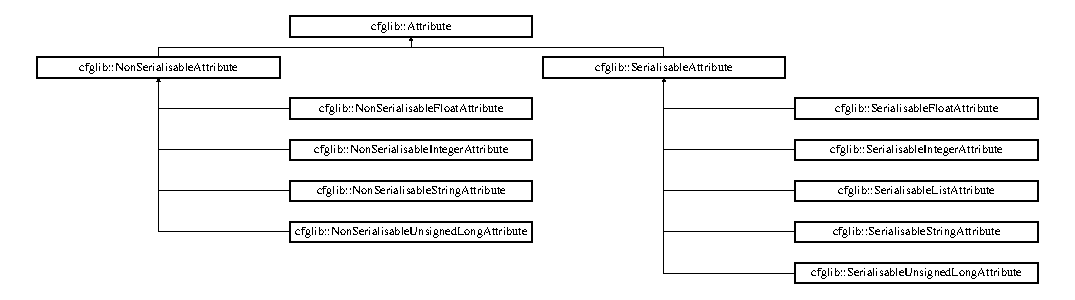
\includegraphics[height=3.589744cm]{classcfglib_1_1Attribute}
\end{center}
\end{figure}
\subsection*{Public Member Functions}
\begin{DoxyCompactItemize}
\item 
\hyperlink{classcfglib_1_1Attribute_ac6c6631f3f1a7077a7f3cdd654f4d194}{Attribute} ()
\item 
virtual \hyperlink{classcfglib_1_1Attribute_af8f971cd97eda6e23c35f1afae0a8c66}{$\sim$\+Attribute} ()
\item 
virtual \hyperlink{classcfglib_1_1Attribute}{Attribute} $\ast$ \hyperlink{classcfglib_1_1Attribute_a107366042fdafe881215426059fec3f8}{clone} ()=0
\item 
virtual \hyperlink{classcfglib_1_1Attribute}{Attribute} $\ast$ \hyperlink{classcfglib_1_1Attribute_a73490b82f9b31d8f30b813a2a9d3fe99}{clone} (\hyperlink{classcfglib_1_1CloneHandle}{Clone\+Handle} \&)
\item 
virtual void \hyperlink{classcfglib_1_1Attribute_af8d87ceddde146b92727e61823e0129b}{Print} (std\+::ostream \&)=0
\item 
void \hyperlink{classcfglib_1_1Attribute_ae6e91c4069d2d54d264e25511e81d962}{Set\+Name} (std\+::string \hyperlink{classcfglib_1_1Attribute_a9abcd440f01bbbc57fc64f274033cd22}{name})
\end{DoxyCompactItemize}
\subsection*{Protected Attributes}
\begin{DoxyCompactItemize}
\item 
std\+::string \hyperlink{classcfglib_1_1Attribute_a9abcd440f01bbbc57fc64f274033cd22}{name}
\end{DoxyCompactItemize}


\subsection{Detailed Description}
Attributes can be attached to any object inheriting from class \hyperlink{classcfglib_1_1Attributed}{Attributed}. Built-\/in attributes are provided by cfglib, and new ones can be defined by its users. Every attribute has a name and a type. An attribute should implement a method clone (attributes are duplicated when attached) and method Print for debugging purposes. Attributes can be serialisable (subclass \hyperlink{classcfglib_1_1SerialisableAttribute}{Serialisable\+Attribute}) or not (subclass \hyperlink{classcfglib_1_1NonSerialisableAttribute}{Non\+Serialisable\+Attribute}). 

\subsection{Constructor \& Destructor Documentation}
\mbox{\Hypertarget{classcfglib_1_1Attribute_ac6c6631f3f1a7077a7f3cdd654f4d194}\label{classcfglib_1_1Attribute_ac6c6631f3f1a7077a7f3cdd654f4d194}} 
\index{cfglib\+::\+Attribute@{cfglib\+::\+Attribute}!Attribute@{Attribute}}
\index{Attribute@{Attribute}!cfglib\+::\+Attribute@{cfglib\+::\+Attribute}}
\subsubsection{\texorpdfstring{Attribute()}{Attribute()}}
{\footnotesize\ttfamily cfglib\+::\+Attribute\+::\+Attribute (\begin{DoxyParamCaption}{ }\end{DoxyParamCaption})\hspace{0.3cm}{\ttfamily [inline]}}

Default constructors and destructors \mbox{\Hypertarget{classcfglib_1_1Attribute_af8f971cd97eda6e23c35f1afae0a8c66}\label{classcfglib_1_1Attribute_af8f971cd97eda6e23c35f1afae0a8c66}} 
\index{cfglib\+::\+Attribute@{cfglib\+::\+Attribute}!````~Attribute@{$\sim$\+Attribute}}
\index{````~Attribute@{$\sim$\+Attribute}!cfglib\+::\+Attribute@{cfglib\+::\+Attribute}}
\subsubsection{\texorpdfstring{$\sim$\+Attribute()}{~Attribute()}}
{\footnotesize\ttfamily virtual cfglib\+::\+Attribute\+::$\sim$\+Attribute (\begin{DoxyParamCaption}{ }\end{DoxyParamCaption})\hspace{0.3cm}{\ttfamily [inline]}, {\ttfamily [virtual]}}



\subsection{Member Function Documentation}
\mbox{\Hypertarget{classcfglib_1_1Attribute_a107366042fdafe881215426059fec3f8}\label{classcfglib_1_1Attribute_a107366042fdafe881215426059fec3f8}} 
\index{cfglib\+::\+Attribute@{cfglib\+::\+Attribute}!clone@{clone}}
\index{clone@{clone}!cfglib\+::\+Attribute@{cfglib\+::\+Attribute}}
\subsubsection{\texorpdfstring{clone()}{clone()}\hspace{0.1cm}{\footnotesize\ttfamily [1/2]}}
{\footnotesize\ttfamily virtual \hyperlink{classcfglib_1_1Attribute}{Attribute}$\ast$ cfglib\+::\+Attribute\+::clone (\begin{DoxyParamCaption}{ }\end{DoxyParamCaption})\hspace{0.3cm}{\ttfamily [pure virtual]}}

\hyperlink{classcfglib_1_1Attribute}{Attribute} cloning function. Used by attribute attachment method Set\+Attribute of class \hyperlink{classcfglib_1_1Attributed}{Attributed} when attaching an attribute to an object deriving from class \hyperlink{classcfglib_1_1Attributed}{Attributed} 

Implemented in \hyperlink{classcfglib_1_1SerialisableListAttribute_a8fe3db52648fbc4d6f08a4bdf7c78ea6}{cfglib\+::\+Serialisable\+List\+Attribute}, \hyperlink{classcfglib_1_1SerialisableUnsignedLongAttribute_a5ddcd35aa3f13ae354bf6dd65839baba}{cfglib\+::\+Serialisable\+Unsigned\+Long\+Attribute}, \hyperlink{classcfglib_1_1NonSerialisableUnsignedLongAttribute_a3c01da3fbc7e617c7a919716a1142f57}{cfglib\+::\+Non\+Serialisable\+Unsigned\+Long\+Attribute}, \hyperlink{classcfglib_1_1SerialisableFloatAttribute_a2addfc6e4ad308e1e84c2b4cdac7636b}{cfglib\+::\+Serialisable\+Float\+Attribute}, \hyperlink{classcfglib_1_1NonSerialisableFloatAttribute_a8cf8fa70d97d003cf48c64c59609eeaf}{cfglib\+::\+Non\+Serialisable\+Float\+Attribute}, \hyperlink{classcfglib_1_1SerialisableIntegerAttribute_a105ce2b9dab265d56bc3229fcb7d6084}{cfglib\+::\+Serialisable\+Integer\+Attribute}, \hyperlink{classcfglib_1_1NonSerialisableIntegerAttribute_ab37d2f2a349d73177e6fdbd1356566ab}{cfglib\+::\+Non\+Serialisable\+Integer\+Attribute}, \hyperlink{classcfglib_1_1SerialisableStringAttribute_a8c1e4b8b3edbb39c85216d2b2cf8ec38}{cfglib\+::\+Serialisable\+String\+Attribute}, and \hyperlink{classcfglib_1_1NonSerialisableStringAttribute_a5a7857efb5a59c478ef31266ddfd2f2c}{cfglib\+::\+Non\+Serialisable\+String\+Attribute}.

\mbox{\Hypertarget{classcfglib_1_1Attribute_a73490b82f9b31d8f30b813a2a9d3fe99}\label{classcfglib_1_1Attribute_a73490b82f9b31d8f30b813a2a9d3fe99}} 
\index{cfglib\+::\+Attribute@{cfglib\+::\+Attribute}!clone@{clone}}
\index{clone@{clone}!cfglib\+::\+Attribute@{cfglib\+::\+Attribute}}
\subsubsection{\texorpdfstring{clone()}{clone()}\hspace{0.1cm}{\footnotesize\ttfamily [2/2]}}
{\footnotesize\ttfamily virtual \hyperlink{classcfglib_1_1Attribute}{Attribute}$\ast$ cfglib\+::\+Attribute\+::clone (\begin{DoxyParamCaption}\item[{\hyperlink{classcfglib_1_1CloneHandle}{Clone\+Handle} \&}]{ }\end{DoxyParamCaption})\hspace{0.3cm}{\ttfamily [inline]}, {\ttfamily [virtual]}}



Reimplemented in \hyperlink{classcfglib_1_1SerialisableListAttribute_a2bcd8907e26992e725a8a10b82288a0f}{cfglib\+::\+Serialisable\+List\+Attribute}.

\mbox{\Hypertarget{classcfglib_1_1Attribute_af8d87ceddde146b92727e61823e0129b}\label{classcfglib_1_1Attribute_af8d87ceddde146b92727e61823e0129b}} 
\index{cfglib\+::\+Attribute@{cfglib\+::\+Attribute}!Print@{Print}}
\index{Print@{Print}!cfglib\+::\+Attribute@{cfglib\+::\+Attribute}}
\subsubsection{\texorpdfstring{Print()}{Print()}}
{\footnotesize\ttfamily virtual void cfglib\+::\+Attribute\+::\+Print (\begin{DoxyParamCaption}\item[{std\+::ostream \&}]{ }\end{DoxyParamCaption})\hspace{0.3cm}{\ttfamily [pure virtual]}}

\hyperlink{classcfglib_1_1Attribute}{Attribute} printing function (used for debug only) 

Implemented in \hyperlink{classcfglib_1_1SerialisableListAttribute_a3a76c800c9ebcd084b64c1c5f049caf5}{cfglib\+::\+Serialisable\+List\+Attribute}, \hyperlink{classcfglib_1_1SerialisableUnsignedLongAttribute_a4d53682ce58f689045c6f55a04e1c6cd}{cfglib\+::\+Serialisable\+Unsigned\+Long\+Attribute}, \hyperlink{classcfglib_1_1NonSerialisableUnsignedLongAttribute_aef0e4a5bc60b6d4f278ab2daa553f598}{cfglib\+::\+Non\+Serialisable\+Unsigned\+Long\+Attribute}, \hyperlink{classcfglib_1_1SerialisableFloatAttribute_af36f296204e1a8547f3fbef7ec4c23da}{cfglib\+::\+Serialisable\+Float\+Attribute}, \hyperlink{classcfglib_1_1NonSerialisableFloatAttribute_a507fc8e93b9ff7c56d483f2e51634e67}{cfglib\+::\+Non\+Serialisable\+Float\+Attribute}, \hyperlink{classcfglib_1_1SerialisableIntegerAttribute_ad2f90817bfc2f4aa2f5be3064e19e11a}{cfglib\+::\+Serialisable\+Integer\+Attribute}, \hyperlink{classcfglib_1_1NonSerialisableIntegerAttribute_ade6c5738723b606295a2cf14fe568247}{cfglib\+::\+Non\+Serialisable\+Integer\+Attribute}, \hyperlink{classcfglib_1_1SerialisableStringAttribute_a7149bb6d92d50db794bde6867cef4550}{cfglib\+::\+Serialisable\+String\+Attribute}, and \hyperlink{classcfglib_1_1NonSerialisableStringAttribute_aedeb7ccd57b84ed2e3bcfc464038682e}{cfglib\+::\+Non\+Serialisable\+String\+Attribute}.

\mbox{\Hypertarget{classcfglib_1_1Attribute_ae6e91c4069d2d54d264e25511e81d962}\label{classcfglib_1_1Attribute_ae6e91c4069d2d54d264e25511e81d962}} 
\index{cfglib\+::\+Attribute@{cfglib\+::\+Attribute}!Set\+Name@{Set\+Name}}
\index{Set\+Name@{Set\+Name}!cfglib\+::\+Attribute@{cfglib\+::\+Attribute}}
\subsubsection{\texorpdfstring{Set\+Name()}{SetName()}}
{\footnotesize\ttfamily void cfglib\+::\+Attribute\+::\+Set\+Name (\begin{DoxyParamCaption}\item[{std\+::string}]{name }\end{DoxyParamCaption})\hspace{0.3cm}{\ttfamily [inline]}}

Set the unique \char`\"{}name\char`\"{} field in a list of \hyperlink{classcfglib_1_1Attribute}{Attribute}. This methos is called during the unserialisation process and not used otherwise 

\subsection{Member Data Documentation}
\mbox{\Hypertarget{classcfglib_1_1Attribute_a9abcd440f01bbbc57fc64f274033cd22}\label{classcfglib_1_1Attribute_a9abcd440f01bbbc57fc64f274033cd22}} 
\index{cfglib\+::\+Attribute@{cfglib\+::\+Attribute}!name@{name}}
\index{name@{name}!cfglib\+::\+Attribute@{cfglib\+::\+Attribute}}
\subsubsection{\texorpdfstring{name}{name}}
{\footnotesize\ttfamily std\+::string cfglib\+::\+Attribute\+::name\hspace{0.3cm}{\ttfamily [protected]}}

There is only one attribute with a given name attached to an \hyperlink{classcfglib_1_1Attributed}{Attributed} object. 

The documentation for this class was generated from the following file\+:\begin{DoxyCompactItemize}
\item 
include/\hyperlink{Attributes_8h}{Attributes.\+h}\end{DoxyCompactItemize}

\hypertarget{classcfglib_1_1Attributed}{}\section{cfglib\+:\+:Attributed Class Reference}
\label{classcfglib_1_1Attributed}\index{cfglib\+::\+Attributed@{cfglib\+::\+Attributed}}


{\ttfamily \#include $<$Attributed.\+h$>$}

Inheritance diagram for cfglib\+:\+:Attributed\+:\begin{figure}[H]
\begin{center}
\leavevmode
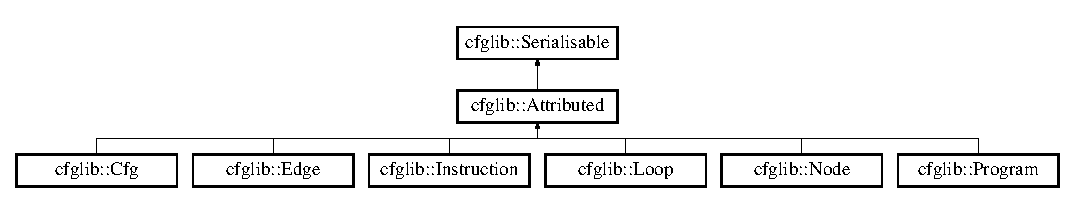
\includegraphics[height=2.276423cm]{classcfglib_1_1Attributed}
\end{center}
\end{figure}
\subsection*{Public Member Functions}
\begin{DoxyCompactItemize}
\item 
bool \hyperlink{classcfglib_1_1Attributed_a7a9a828f1cd9fcd11bfcb5bed166d132}{Has\+Attribute} (std\+::string symbol)
\item 
\hyperlink{classcfglib_1_1Attribute}{Attribute} \& \hyperlink{classcfglib_1_1Attributed_a78db2f7e006d00bf860b32761ec2c88d}{Get\+Attribute} (std\+::string symbol)
\item 
std\+::vector$<$ string $>$ \hyperlink{classcfglib_1_1Attributed_ab61bf9157b32995f4b0dfcc61cc0b35b}{get\+Attribute\+List} (void)
\item 
void \hyperlink{classcfglib_1_1Attributed_aa0bca88f8daee79c5ab66883608e700c}{Clone\+Attributes\+For} (\hyperlink{classcfglib_1_1Attributed}{Attributed} $\ast$, \hyperlink{classcfglib_1_1CloneHandle}{Clone\+Handle} \&)
\item 
void \hyperlink{classcfglib_1_1Attributed_a354c313adbd2b325718c2e3c3127edc6}{Set\+Attribute} (std\+::string const \&symbol, \hyperlink{classcfglib_1_1Attribute}{Attribute} \&attribute)
\item 
void \hyperlink{classcfglib_1_1Attributed_a725edd325af54006acfb25b4cf8760fd}{Remove\+Attribute} (std\+::string const \&symbol)
\item 
void \hyperlink{classcfglib_1_1Attributed_a8952d975e36fc5d1a824ff0d27dfc0df}{Print\+Non\+Serialisable\+Attributes} (std\+::ostream \&os)
\item 
std\+::ostream \& \hyperlink{classcfglib_1_1Attributed_af1cf65adeb481619018088533a7dc306}{Write\+Xml\+Attributes} (std\+::ostream \&os, \hyperlink{classcfglib_1_1Handle}{Handle} \&hand\+\_\+ser) const
\item 
void \hyperlink{classcfglib_1_1Attributed_afd7bf0f8c2321dbd5c7206ece7da1393}{Read\+Xml\+Attributes} (\hyperlink{classXmlTag}{Xml\+Tag} const $\ast$tag, \hyperlink{classcfglib_1_1Handle}{Handle} \&hand)
\item 
virtual \hyperlink{classcfglib_1_1Attributed_adb9f15c2776aa3976b5a3eff54d3cde7}{$\sim$\+Attributed} ()
\end{DoxyCompactItemize}


\subsection{Detailed Description}
\hyperlink{classcfglib_1_1Attributed}{Attributed}. All objects to which we can add attributes inherit this class. 

\subsection{Constructor \& Destructor Documentation}
\mbox{\Hypertarget{classcfglib_1_1Attributed_adb9f15c2776aa3976b5a3eff54d3cde7}\label{classcfglib_1_1Attributed_adb9f15c2776aa3976b5a3eff54d3cde7}} 
\index{cfglib\+::\+Attributed@{cfglib\+::\+Attributed}!````~Attributed@{$\sim$\+Attributed}}
\index{````~Attributed@{$\sim$\+Attributed}!cfglib\+::\+Attributed@{cfglib\+::\+Attributed}}
\subsubsection{\texorpdfstring{$\sim$\+Attributed()}{~Attributed()}}
{\footnotesize\ttfamily virtual cfglib\+::\+Attributed\+::$\sim$\+Attributed (\begin{DoxyParamCaption}{ }\end{DoxyParamCaption})\hspace{0.3cm}{\ttfamily [virtual]}}

virtual destructor. 

\subsection{Member Function Documentation}
\mbox{\Hypertarget{classcfglib_1_1Attributed_aa0bca88f8daee79c5ab66883608e700c}\label{classcfglib_1_1Attributed_aa0bca88f8daee79c5ab66883608e700c}} 
\index{cfglib\+::\+Attributed@{cfglib\+::\+Attributed}!Clone\+Attributes\+For@{Clone\+Attributes\+For}}
\index{Clone\+Attributes\+For@{Clone\+Attributes\+For}!cfglib\+::\+Attributed@{cfglib\+::\+Attributed}}
\subsubsection{\texorpdfstring{Clone\+Attributes\+For()}{CloneAttributesFor()}}
{\footnotesize\ttfamily void cfglib\+::\+Attributed\+::\+Clone\+Attributes\+For (\begin{DoxyParamCaption}\item[{\hyperlink{classcfglib_1_1Attributed}{Attributed} $\ast$}]{,  }\item[{\hyperlink{classcfglib_1_1CloneHandle}{Clone\+Handle} \&}]{ }\end{DoxyParamCaption})}

\mbox{\Hypertarget{classcfglib_1_1Attributed_a78db2f7e006d00bf860b32761ec2c88d}\label{classcfglib_1_1Attributed_a78db2f7e006d00bf860b32761ec2c88d}} 
\index{cfglib\+::\+Attributed@{cfglib\+::\+Attributed}!Get\+Attribute@{Get\+Attribute}}
\index{Get\+Attribute@{Get\+Attribute}!cfglib\+::\+Attributed@{cfglib\+::\+Attributed}}
\subsubsection{\texorpdfstring{Get\+Attribute()}{GetAttribute()}}
{\footnotesize\ttfamily \hyperlink{classcfglib_1_1Attribute}{Attribute}\& cfglib\+::\+Attributed\+::\+Get\+Attribute (\begin{DoxyParamCaption}\item[{std\+::string}]{symbol }\end{DoxyParamCaption})}

Get a attribute given its name. The method makes a copy of the attribute by calling its method \char`\"{}clone\char`\"{} before the attribute is stored. All attributed must have a \textquotesingle{}clone\textquotesingle{} method implemented. Method Has\+Attribute has to be called before trying to retrieve an attribute to make sure the attribute with name \textquotesingle{}symbol\textquotesingle{} exists (else, an assertion in the code fails). In the case the attribute contains pointers on other attributes, the attribute copy constructor has to be defined. Example of use of attributes (with n an attributed object) Integer\+Attribute ia(6); // Declare an integer attribute n.\+Set\+Attribute(\char`\"{}myinteger\char`\"{},ia); // Attach a copy of the attribute to object n

Integer\+Attribute ia; // Declare an attribute assert(n.\+Has\+Attribute(\char`\"{}myinteger\char`\"{});// Make sure n has an attribute attached ia=n.\+Get\+Attribute(\char`\"{}myinteger\char`\"{}); // Retrieve a copy of the attribute in ia int val = ia.\+Get\+Value(); // Get it\textquotesingle{}s value (here, a simple integer) \mbox{\Hypertarget{classcfglib_1_1Attributed_ab61bf9157b32995f4b0dfcc61cc0b35b}\label{classcfglib_1_1Attributed_ab61bf9157b32995f4b0dfcc61cc0b35b}} 
\index{cfglib\+::\+Attributed@{cfglib\+::\+Attributed}!get\+Attribute\+List@{get\+Attribute\+List}}
\index{get\+Attribute\+List@{get\+Attribute\+List}!cfglib\+::\+Attributed@{cfglib\+::\+Attributed}}
\subsubsection{\texorpdfstring{get\+Attribute\+List()}{getAttributeList()}}
{\footnotesize\ttfamily std\+::vector$<$string$>$ cfglib\+::\+Attributed\+::get\+Attribute\+List (\begin{DoxyParamCaption}\item[{void}]{ }\end{DoxyParamCaption})}

return every symbols used in the attribute map \mbox{\Hypertarget{classcfglib_1_1Attributed_a7a9a828f1cd9fcd11bfcb5bed166d132}\label{classcfglib_1_1Attributed_a7a9a828f1cd9fcd11bfcb5bed166d132}} 
\index{cfglib\+::\+Attributed@{cfglib\+::\+Attributed}!Has\+Attribute@{Has\+Attribute}}
\index{Has\+Attribute@{Has\+Attribute}!cfglib\+::\+Attributed@{cfglib\+::\+Attributed}}
\subsubsection{\texorpdfstring{Has\+Attribute()}{HasAttribute()}}
{\footnotesize\ttfamily bool cfglib\+::\+Attributed\+::\+Has\+Attribute (\begin{DoxyParamCaption}\item[{std\+::string}]{symbol }\end{DoxyParamCaption})}

Returns true if the attributed object has an attribute of name \textquotesingle{}symbol\textquotesingle{} attached Must be called before any attempt to call method Get\+Attribute \mbox{\Hypertarget{classcfglib_1_1Attributed_a8952d975e36fc5d1a824ff0d27dfc0df}\label{classcfglib_1_1Attributed_a8952d975e36fc5d1a824ff0d27dfc0df}} 
\index{cfglib\+::\+Attributed@{cfglib\+::\+Attributed}!Print\+Non\+Serialisable\+Attributes@{Print\+Non\+Serialisable\+Attributes}}
\index{Print\+Non\+Serialisable\+Attributes@{Print\+Non\+Serialisable\+Attributes}!cfglib\+::\+Attributed@{cfglib\+::\+Attributed}}
\subsubsection{\texorpdfstring{Print\+Non\+Serialisable\+Attributes()}{PrintNonSerialisableAttributes()}}
{\footnotesize\ttfamily void cfglib\+::\+Attributed\+::\+Print\+Non\+Serialisable\+Attributes (\begin{DoxyParamCaption}\item[{std\+::ostream \&}]{os }\end{DoxyParamCaption})}

Print information on the non serialisable attributes, by calling their Print method. Used for debug only, to check that all Non\+Serialisable\+Attributes are removed at the end of every analysis. \mbox{\Hypertarget{classcfglib_1_1Attributed_afd7bf0f8c2321dbd5c7206ece7da1393}\label{classcfglib_1_1Attributed_afd7bf0f8c2321dbd5c7206ece7da1393}} 
\index{cfglib\+::\+Attributed@{cfglib\+::\+Attributed}!Read\+Xml\+Attributes@{Read\+Xml\+Attributes}}
\index{Read\+Xml\+Attributes@{Read\+Xml\+Attributes}!cfglib\+::\+Attributed@{cfglib\+::\+Attributed}}
\subsubsection{\texorpdfstring{Read\+Xml\+Attributes()}{ReadXmlAttributes()}}
{\footnotesize\ttfamily void cfglib\+::\+Attributed\+::\+Read\+Xml\+Attributes (\begin{DoxyParamCaption}\item[{\hyperlink{classXmlTag}{Xml\+Tag} const $\ast$}]{tag,  }\item[{\hyperlink{classcfglib_1_1Handle}{Handle} \&}]{hand }\end{DoxyParamCaption})}

Unserialise all attributes \mbox{\Hypertarget{classcfglib_1_1Attributed_a725edd325af54006acfb25b4cf8760fd}\label{classcfglib_1_1Attributed_a725edd325af54006acfb25b4cf8760fd}} 
\index{cfglib\+::\+Attributed@{cfglib\+::\+Attributed}!Remove\+Attribute@{Remove\+Attribute}}
\index{Remove\+Attribute@{Remove\+Attribute}!cfglib\+::\+Attributed@{cfglib\+::\+Attributed}}
\subsubsection{\texorpdfstring{Remove\+Attribute()}{RemoveAttribute()}}
{\footnotesize\ttfamily void cfglib\+::\+Attributed\+::\+Remove\+Attribute (\begin{DoxyParamCaption}\item[{std\+::string const \&}]{symbol }\end{DoxyParamCaption})}

Remove an attribute (frees its memory) (if not removed, an attribute stays attached and consumes memory up to the program termination) \mbox{\Hypertarget{classcfglib_1_1Attributed_a354c313adbd2b325718c2e3c3127edc6}\label{classcfglib_1_1Attributed_a354c313adbd2b325718c2e3c3127edc6}} 
\index{cfglib\+::\+Attributed@{cfglib\+::\+Attributed}!Set\+Attribute@{Set\+Attribute}}
\index{Set\+Attribute@{Set\+Attribute}!cfglib\+::\+Attributed@{cfglib\+::\+Attributed}}
\subsubsection{\texorpdfstring{Set\+Attribute()}{SetAttribute()}}
{\footnotesize\ttfamily void cfglib\+::\+Attributed\+::\+Set\+Attribute (\begin{DoxyParamCaption}\item[{std\+::string const \&}]{symbol,  }\item[{\hyperlink{classcfglib_1_1Attribute}{Attribute} \&}]{attribute }\end{DoxyParamCaption})}

Add or replace a named attribute. A pointer to a copy of the attribute is stored. In case an already existing attribute is replaced, the attribute is deleted before the new one is installed. \mbox{\Hypertarget{classcfglib_1_1Attributed_af1cf65adeb481619018088533a7dc306}\label{classcfglib_1_1Attributed_af1cf65adeb481619018088533a7dc306}} 
\index{cfglib\+::\+Attributed@{cfglib\+::\+Attributed}!Write\+Xml\+Attributes@{Write\+Xml\+Attributes}}
\index{Write\+Xml\+Attributes@{Write\+Xml\+Attributes}!cfglib\+::\+Attributed@{cfglib\+::\+Attributed}}
\subsubsection{\texorpdfstring{Write\+Xml\+Attributes()}{WriteXmlAttributes()}}
{\footnotesize\ttfamily std\+::ostream\& cfglib\+::\+Attributed\+::\+Write\+Xml\+Attributes (\begin{DoxyParamCaption}\item[{std\+::ostream \&}]{os,  }\item[{\hyperlink{classcfglib_1_1Handle}{Handle} \&}]{hand\+\_\+ser }\end{DoxyParamCaption}) const}

Serialise all attributes 

The documentation for this class was generated from the following file\+:\begin{DoxyCompactItemize}
\item 
include/\hyperlink{Attributed_8h}{Attributed.\+h}\end{DoxyCompactItemize}

\hypertarget{classcfglib_1_1AttributesFactory}{}\section{cfglib\+:\+:Attributes\+Factory Class Reference}
\label{classcfglib_1_1AttributesFactory}\index{cfglib\+::\+Attributes\+Factory@{cfglib\+::\+Attributes\+Factory}}


{\ttfamily \#include $<$Factory.\+h$>$}

\subsection*{Public Member Functions}
\begin{DoxyCompactItemize}
\item 
\hyperlink{classcfglib_1_1SerialisableAttribute}{Serialisable\+Attribute} $\ast$ \hyperlink{classcfglib_1_1AttributesFactory_a28cadc5986575e1f99dee0611aadf46d}{Create\+New\+Attribute} (std\+::string const \&type)
\item 
void \hyperlink{classcfglib_1_1AttributesFactory_a409fa8a154e72a1041438c6e278bd502}{Set\+Attribute\+Type} (std\+::string const \&, \hyperlink{classcfglib_1_1SerialisableAttribute}{Serialisable\+Attribute} $\ast$)
\end{DoxyCompactItemize}
\subsection*{Static Public Member Functions}
\begin{DoxyCompactItemize}
\item 
static \hyperlink{classcfglib_1_1AttributesFactory}{Attributes\+Factory} $\ast$ \hyperlink{classcfglib_1_1AttributesFactory_a467b197e6a1dbbdcece13c93766a19ee}{Get\+Instance} ()
\item 
static void \hyperlink{classcfglib_1_1AttributesFactory_a3a1adf8be0c0115a191837d6c085c928}{Kill\+Instance} ()
\end{DoxyCompactItemize}


\subsection{Member Function Documentation}
\mbox{\Hypertarget{classcfglib_1_1AttributesFactory_a28cadc5986575e1f99dee0611aadf46d}\label{classcfglib_1_1AttributesFactory_a28cadc5986575e1f99dee0611aadf46d}} 
\index{cfglib\+::\+Attributes\+Factory@{cfglib\+::\+Attributes\+Factory}!Create\+New\+Attribute@{Create\+New\+Attribute}}
\index{Create\+New\+Attribute@{Create\+New\+Attribute}!cfglib\+::\+Attributes\+Factory@{cfglib\+::\+Attributes\+Factory}}
\subsubsection{\texorpdfstring{Create\+New\+Attribute()}{CreateNewAttribute()}}
{\footnotesize\ttfamily \hyperlink{classcfglib_1_1SerialisableAttribute}{Serialisable\+Attribute}$\ast$ cfglib\+::\+Attributes\+Factory\+::\+Create\+New\+Attribute (\begin{DoxyParamCaption}\item[{std\+::string const \&}]{type }\end{DoxyParamCaption})}

creation of attribute of a given type. \mbox{\Hypertarget{classcfglib_1_1AttributesFactory_a467b197e6a1dbbdcece13c93766a19ee}\label{classcfglib_1_1AttributesFactory_a467b197e6a1dbbdcece13c93766a19ee}} 
\index{cfglib\+::\+Attributes\+Factory@{cfglib\+::\+Attributes\+Factory}!Get\+Instance@{Get\+Instance}}
\index{Get\+Instance@{Get\+Instance}!cfglib\+::\+Attributes\+Factory@{cfglib\+::\+Attributes\+Factory}}
\subsubsection{\texorpdfstring{Get\+Instance()}{GetInstance()}}
{\footnotesize\ttfamily static \hyperlink{classcfglib_1_1AttributesFactory}{Attributes\+Factory}$\ast$ cfglib\+::\+Attributes\+Factory\+::\+Get\+Instance (\begin{DoxyParamCaption}{ }\end{DoxyParamCaption})\hspace{0.3cm}{\ttfamily [static]}}

Access to global attribute factory \mbox{\Hypertarget{classcfglib_1_1AttributesFactory_a3a1adf8be0c0115a191837d6c085c928}\label{classcfglib_1_1AttributesFactory_a3a1adf8be0c0115a191837d6c085c928}} 
\index{cfglib\+::\+Attributes\+Factory@{cfglib\+::\+Attributes\+Factory}!Kill\+Instance@{Kill\+Instance}}
\index{Kill\+Instance@{Kill\+Instance}!cfglib\+::\+Attributes\+Factory@{cfglib\+::\+Attributes\+Factory}}
\subsubsection{\texorpdfstring{Kill\+Instance()}{KillInstance()}}
{\footnotesize\ttfamily static void cfglib\+::\+Attributes\+Factory\+::\+Kill\+Instance (\begin{DoxyParamCaption}{ }\end{DoxyParamCaption})\hspace{0.3cm}{\ttfamily [static]}}

Declare end of access of attribute factory \mbox{\Hypertarget{classcfglib_1_1AttributesFactory_a409fa8a154e72a1041438c6e278bd502}\label{classcfglib_1_1AttributesFactory_a409fa8a154e72a1041438c6e278bd502}} 
\index{cfglib\+::\+Attributes\+Factory@{cfglib\+::\+Attributes\+Factory}!Set\+Attribute\+Type@{Set\+Attribute\+Type}}
\index{Set\+Attribute\+Type@{Set\+Attribute\+Type}!cfglib\+::\+Attributes\+Factory@{cfglib\+::\+Attributes\+Factory}}
\subsubsection{\texorpdfstring{Set\+Attribute\+Type()}{SetAttributeType()}}
{\footnotesize\ttfamily void cfglib\+::\+Attributes\+Factory\+::\+Set\+Attribute\+Type (\begin{DoxyParamCaption}\item[{std\+::string const \&}]{,  }\item[{\hyperlink{classcfglib_1_1SerialisableAttribute}{Serialisable\+Attribute} $\ast$}]{ }\end{DoxyParamCaption})}

association between a type identifier and a constructor function. 

The documentation for this class was generated from the following file\+:\begin{DoxyCompactItemize}
\item 
include/\hyperlink{Factory_8h}{Factory.\+h}\end{DoxyCompactItemize}

\hypertarget{classcfglib_1_1Cfg}{}\section{cfglib\+:\+:Cfg Class Reference}
\label{classcfglib_1_1Cfg}\index{cfglib\+::\+Cfg@{cfglib\+::\+Cfg}}


{\ttfamily \#include $<$Cfg.\+h$>$}

Inheritance diagram for cfglib\+:\+:Cfg\+:\begin{figure}[H]
\begin{center}
\leavevmode
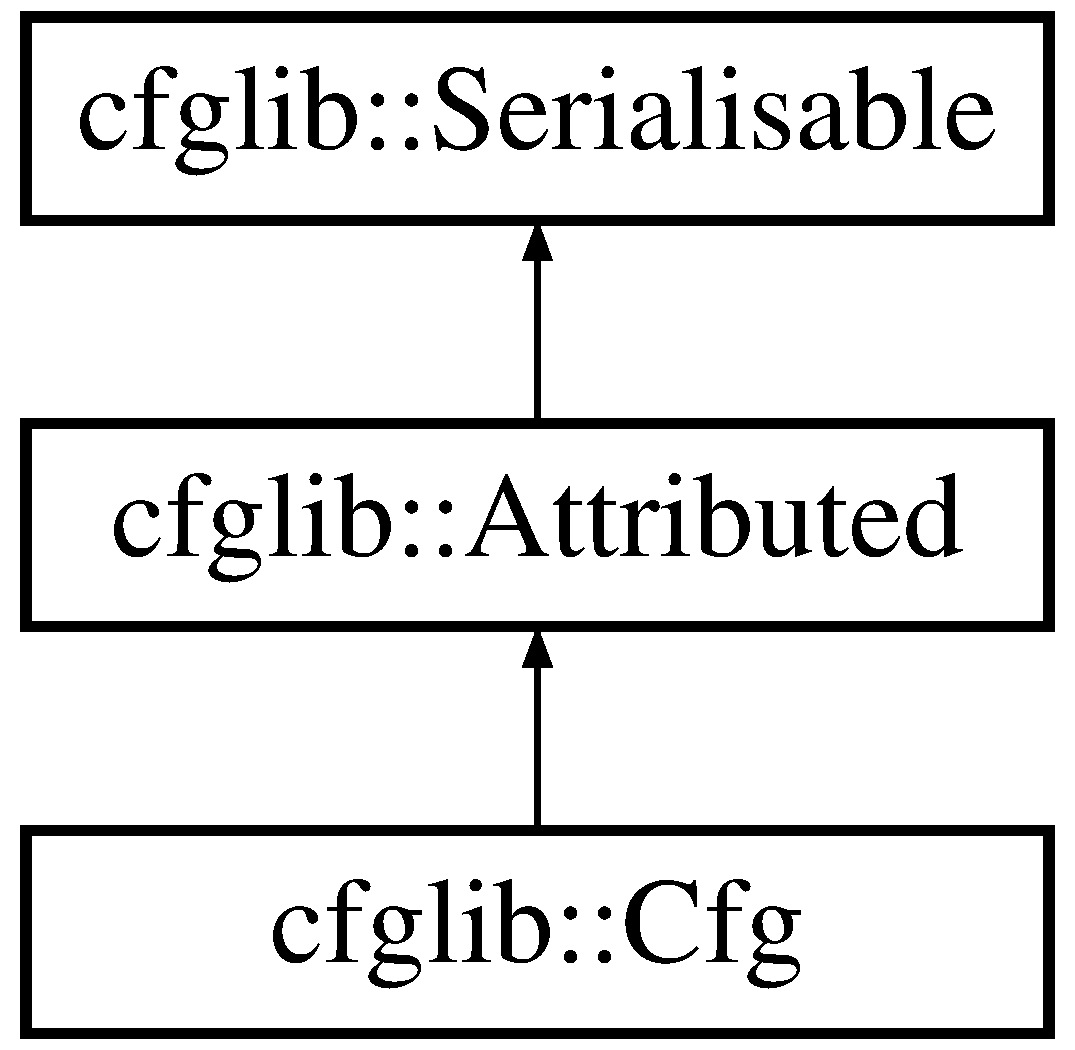
\includegraphics[height=3.000000cm]{classcfglib_1_1Cfg}
\end{center}
\end{figure}
\subsection*{Public Member Functions}
\begin{DoxyCompactItemize}
\item 
\hyperlink{classcfglib_1_1Cfg_a0100bef586e13e2ad53c83b20e365c5e}{Cfg} (\hyperlink{classcfglib_1_1Program}{Program} $\ast$program, List\+Of\+String name)
\item 
\hyperlink{classcfglib_1_1Cfg_a3c7102871bcac1c06389aa38674c76b1}{Cfg} (List\+Of\+String name)
\item 
\hyperlink{classcfglib_1_1Cfg_a279b0b9b7f73a621bc50b35cf7fb7dda}{$\sim$\+Cfg} ()
\item 
\hyperlink{classcfglib_1_1Cfg}{Cfg} $\ast$ \hyperlink{classcfglib_1_1Cfg_a87e8932c31bd9747af7eafc92b6d749b}{Clone} (\hyperlink{classcfglib_1_1CloneHandle}{Clone\+Handle} \&)
\item 
List\+Of\+String \hyperlink{classcfglib_1_1Cfg_a429688de55701afc5e5e41a6cfcae050}{Get\+Name} ()
\item 
bool \hyperlink{classcfglib_1_1Cfg_a53c796e515ba5bdad1dd17b5e2cea403}{Is\+External} () const
\item 
\hyperlink{classcfglib_1_1Program}{Program} $\ast$ \hyperlink{classcfglib_1_1Cfg_aefc6931e39418420ae47e09528bba5af}{Get\+Program} ()
\item 
void \hyperlink{classcfglib_1_1Cfg_a6408b372beac5ab2eaa02dbea18ca23c}{Set\+Program} (\hyperlink{classcfglib_1_1Program}{Program} $\ast$p)
\item 
std\+::vector$<$ \hyperlink{classcfglib_1_1Node}{Node} $\ast$ $>$ \hyperlink{classcfglib_1_1Cfg_a54ab52821050574fa12eca0eb87f7271}{Get\+Call\+Nodes} (void)
\item 
bool \hyperlink{classcfglib_1_1Cfg_a09c2fff20ceddf2a659bbc8e64559f8e}{Is\+Empty} () const
\item 
\hyperlink{classcfglib_1_1Node}{Node} $\ast$ \hyperlink{classcfglib_1_1Cfg_a023e8fe06cf55bfecf3c1f4a3ddb3f99}{Create\+New\+Node} (enum \hyperlink{namespacecfglib_a44952a45d827aaa271f7e7dac5bf7752}{node\+\_\+type} type)
\item 
\hyperlink{classcfglib_1_1Edge}{Edge} $\ast$ \hyperlink{classcfglib_1_1Cfg_aa3e584ba98c948fe9cb31cbd9ba30215}{Create\+New\+Edge} (\hyperlink{classcfglib_1_1Node}{Node} $\ast$origin, \hyperlink{classcfglib_1_1Node}{Node} $\ast$destination)
\item 
void \hyperlink{classcfglib_1_1Cfg_a4150c4a82a82d63ab855595c844148f2}{Remove\+Edge} (\hyperlink{classcfglib_1_1Edge}{Edge} $\ast$e)
\item 
void \hyperlink{classcfglib_1_1Cfg_acebbb5cb49f9cf8c50ffe0918cbd98d1}{Remove\+Edge\+No\+Delete} (\hyperlink{classcfglib_1_1Edge}{Edge} $\ast$e)
\item 
void \hyperlink{classcfglib_1_1Cfg_aca4049e467e6979666c3273bf3e3045a}{put\+Edge} (\hyperlink{classcfglib_1_1Edge}{Edge} $\ast$E)
\item 
std\+::vector$<$ \hyperlink{classcfglib_1_1Node}{Node} $\ast$ $>$ \hyperlink{classcfglib_1_1Cfg_a0a5b78a124083bb3419d10968de0554a}{Get\+All\+Nodes} ()
\item 
std\+::vector$<$ \hyperlink{classcfglib_1_1Edge}{Edge} $\ast$ $>$ \hyperlink{classcfglib_1_1Cfg_aae35959d564c688ffe76f3d121c47447}{Get\+All\+Edges} ()
\item 
std\+::vector$<$ \hyperlink{classcfglib_1_1Loop}{Loop} $\ast$ $>$ \hyperlink{classcfglib_1_1Cfg_ac5e6efa01325b49924190a1f89727ed5}{Get\+All\+Loops} ()
\item 
\hyperlink{classcfglib_1_1Edge}{Edge} $\ast$ \hyperlink{classcfglib_1_1Cfg_a89f9917fc598d5782698823d2d006782}{Find\+Edge} (\hyperlink{classcfglib_1_1Node}{Node} const $\ast$origin, \hyperlink{classcfglib_1_1Node}{Node} const $\ast$destination) const
\item 
\hyperlink{classcfglib_1_1Node}{Node} $\ast$ \hyperlink{classcfglib_1_1Cfg_ae3c864797fe19d85c1ab303baa7e9fbb}{Get\+Start\+Node} ()
\item 
void \hyperlink{classcfglib_1_1Cfg_ad77f85cebfb1ef7e55afa78f48b6f96e}{Set\+Start\+Node} (\hyperlink{classcfglib_1_1Node}{Node} $\ast$node)
\item 
std\+::vector$<$ \hyperlink{classcfglib_1_1Node}{Node} $\ast$ $>$ \hyperlink{classcfglib_1_1Cfg_aa94cd8bb8d1d33cdcd6d1a7e0b244370}{Get\+End\+Nodes} ()
\item 
void \hyperlink{classcfglib_1_1Cfg_ae235a54ff74dd424c6b5d582ce670c5b}{Set\+End\+Node} (\hyperlink{classcfglib_1_1Node}{Node} $\ast$node)
\item 
void \hyperlink{classcfglib_1_1Cfg_a892063ed55599c1618e49dd31555e7fb}{remove\+End\+Node} (\hyperlink{classcfglib_1_1Node}{Node} $\ast$node)
\item 
std\+::vector$<$ \hyperlink{classcfglib_1_1Edge}{Edge} $\ast$ $>$ \hyperlink{classcfglib_1_1Cfg_ac87776adfdc86881d01c4ea529004c1a}{Get\+Incoming\+Edges} (\hyperlink{classcfglib_1_1Node}{Node} $\ast$node)
\item 
std\+::vector$<$ \hyperlink{classcfglib_1_1Node}{Node} $\ast$ $>$ \hyperlink{classcfglib_1_1Cfg_ac5fcaa98be7d92862fa1cfa12bc539e6}{Get\+Predecessors} (\hyperlink{classcfglib_1_1Node}{Node} $\ast$node)
\item 
std\+::vector$<$ \hyperlink{classcfglib_1_1Edge}{Edge} $\ast$ $>$ \hyperlink{classcfglib_1_1Cfg_aea82731a4de76ef618bc91e8ab11c56b}{Get\+Outgoing\+Edges} (\hyperlink{classcfglib_1_1Node}{Node} $\ast$node)
\item 
std\+::vector$<$ \hyperlink{classcfglib_1_1Node}{Node} $\ast$ $>$ \hyperlink{classcfglib_1_1Cfg_a4f52a0e3814e4d404d5520437d27d407}{Get\+Successors} (\hyperlink{classcfglib_1_1Node}{Node} $\ast$node)
\item 
\hyperlink{classcfglib_1_1Node}{Node} $\ast$ \hyperlink{classcfglib_1_1Cfg_a1b40c4d28399a71195159b3fc1057399}{Get\+Source\+Node} (\hyperlink{classcfglib_1_1Edge}{Edge} $\ast$edge)
\item 
\hyperlink{classcfglib_1_1Node}{Node} $\ast$ \hyperlink{classcfglib_1_1Cfg_aaf238d539a151d6087a9381f5a89555e}{Get\+Target\+Node} (\hyperlink{classcfglib_1_1Edge}{Edge} $\ast$edge)
\item 
\hyperlink{classcfglib_1_1Loop}{Loop} $\ast$ \hyperlink{classcfglib_1_1Cfg_a5c751a3e53b10ecdae556b2936e5303c}{Create\+New\+Loop} (\hyperlink{classcfglib_1_1Node}{Node} $\ast$start\+Node, std\+::vector$<$ \hyperlink{classcfglib_1_1Node}{Node} $\ast$$>$ const \&other\+Nodes\+List)
\item 
\hyperlink{classcfglib_1_1Loop}{Loop} $\ast$ \hyperlink{classcfglib_1_1Cfg_af8e183cfc272143b47dc856f8f368627}{Create\+New\+Loop} ()
\item 
void \hyperlink{classcfglib_1_1Cfg_a4c71befb94beac37921b82361825cc54}{Remove\+Loop} (\hyperlink{classcfglib_1_1Loop}{Loop} $\ast$loop)
\item 
std\+::ostream \& \hyperlink{classcfglib_1_1Cfg_a05c9fc4c8a7e5c0850e6998722433787}{Write\+Xml} (std\+::ostream \&oss, \hyperlink{classcfglib_1_1Handle}{Handle} \&hand)
\item 
virtual void \hyperlink{classcfglib_1_1Cfg_a3525e0c748971e945193da2a0dd4b571}{Read\+Xml} (\hyperlink{classXmlTag}{Xml\+Tag} const $\ast$tag, \hyperlink{classcfglib_1_1Handle}{Handle} \&hand)
\item 
string \hyperlink{classcfglib_1_1Cfg_ae9317f335c39263f55484b0149725d4c}{get\+String\+Name} ()
\item 
void \hyperlink{classcfglib_1_1Cfg_ad939d89b58f8de319335e307069ae2ab}{Yixian\+Test\+Name} ()
\end{DoxyCompactItemize}


\subsection{Detailed Description}
This class represents a Control Flow Graph. 

\subsection{Constructor \& Destructor Documentation}
\mbox{\Hypertarget{classcfglib_1_1Cfg_a0100bef586e13e2ad53c83b20e365c5e}\label{classcfglib_1_1Cfg_a0100bef586e13e2ad53c83b20e365c5e}} 
\index{cfglib\+::\+Cfg@{cfglib\+::\+Cfg}!Cfg@{Cfg}}
\index{Cfg@{Cfg}!cfglib\+::\+Cfg@{cfglib\+::\+Cfg}}
\subsubsection{\texorpdfstring{Cfg()}{Cfg()}\hspace{0.1cm}{\footnotesize\ttfamily [1/2]}}
{\footnotesize\ttfamily cfglib\+::\+Cfg\+::\+Cfg (\begin{DoxyParamCaption}\item[{\hyperlink{classcfglib_1_1Program}{Program} $\ast$}]{program,  }\item[{List\+Of\+String}]{name }\end{DoxyParamCaption})}

Basic constructor. \mbox{\Hypertarget{classcfglib_1_1Cfg_a3c7102871bcac1c06389aa38674c76b1}\label{classcfglib_1_1Cfg_a3c7102871bcac1c06389aa38674c76b1}} 
\index{cfglib\+::\+Cfg@{cfglib\+::\+Cfg}!Cfg@{Cfg}}
\index{Cfg@{Cfg}!cfglib\+::\+Cfg@{cfglib\+::\+Cfg}}
\subsubsection{\texorpdfstring{Cfg()}{Cfg()}\hspace{0.1cm}{\footnotesize\ttfamily [2/2]}}
{\footnotesize\ttfamily cfglib\+::\+Cfg\+::\+Cfg (\begin{DoxyParamCaption}\item[{List\+Of\+String}]{name }\end{DoxyParamCaption})}

constructor for a free \hyperlink{classcfglib_1_1Cfg}{Cfg} (used in clone function) \mbox{\Hypertarget{classcfglib_1_1Cfg_a279b0b9b7f73a621bc50b35cf7fb7dda}\label{classcfglib_1_1Cfg_a279b0b9b7f73a621bc50b35cf7fb7dda}} 
\index{cfglib\+::\+Cfg@{cfglib\+::\+Cfg}!````~Cfg@{$\sim$\+Cfg}}
\index{````~Cfg@{$\sim$\+Cfg}!cfglib\+::\+Cfg@{cfglib\+::\+Cfg}}
\subsubsection{\texorpdfstring{$\sim$\+Cfg()}{~Cfg()}}
{\footnotesize\ttfamily cfglib\+::\+Cfg\+::$\sim$\+Cfg (\begin{DoxyParamCaption}{ }\end{DoxyParamCaption})}

destructor 

\subsection{Member Function Documentation}
\mbox{\Hypertarget{classcfglib_1_1Cfg_a87e8932c31bd9747af7eafc92b6d749b}\label{classcfglib_1_1Cfg_a87e8932c31bd9747af7eafc92b6d749b}} 
\index{cfglib\+::\+Cfg@{cfglib\+::\+Cfg}!Clone@{Clone}}
\index{Clone@{Clone}!cfglib\+::\+Cfg@{cfglib\+::\+Cfg}}
\subsubsection{\texorpdfstring{Clone()}{Clone()}}
{\footnotesize\ttfamily \hyperlink{classcfglib_1_1Cfg}{Cfg}$\ast$ cfglib\+::\+Cfg\+::\+Clone (\begin{DoxyParamCaption}\item[{\hyperlink{classcfglib_1_1CloneHandle}{Clone\+Handle} \&}]{ }\end{DoxyParamCaption})}

Cloning function The program in which this C\+FG is associated have to be set manualy (use the \hyperlink{classcfglib_1_1Cfg_a6408b372beac5ab2eaa02dbea18ca23c}{Cfg\+::\+Set\+Program(\+Program$\ast$ P)} function) \mbox{\Hypertarget{classcfglib_1_1Cfg_aa3e584ba98c948fe9cb31cbd9ba30215}\label{classcfglib_1_1Cfg_aa3e584ba98c948fe9cb31cbd9ba30215}} 
\index{cfglib\+::\+Cfg@{cfglib\+::\+Cfg}!Create\+New\+Edge@{Create\+New\+Edge}}
\index{Create\+New\+Edge@{Create\+New\+Edge}!cfglib\+::\+Cfg@{cfglib\+::\+Cfg}}
\subsubsection{\texorpdfstring{Create\+New\+Edge()}{CreateNewEdge()}}
{\footnotesize\ttfamily \hyperlink{classcfglib_1_1Edge}{Edge}$\ast$ cfglib\+::\+Cfg\+::\+Create\+New\+Edge (\begin{DoxyParamCaption}\item[{\hyperlink{classcfglib_1_1Node}{Node} $\ast$}]{origin,  }\item[{\hyperlink{classcfglib_1_1Node}{Node} $\ast$}]{destination }\end{DoxyParamCaption})}

Adding an edge. Given two nodes, create an edge from the first to the second. This edge must not yet exist. \mbox{\Hypertarget{classcfglib_1_1Cfg_a5c751a3e53b10ecdae556b2936e5303c}\label{classcfglib_1_1Cfg_a5c751a3e53b10ecdae556b2936e5303c}} 
\index{cfglib\+::\+Cfg@{cfglib\+::\+Cfg}!Create\+New\+Loop@{Create\+New\+Loop}}
\index{Create\+New\+Loop@{Create\+New\+Loop}!cfglib\+::\+Cfg@{cfglib\+::\+Cfg}}
\subsubsection{\texorpdfstring{Create\+New\+Loop()}{CreateNewLoop()}\hspace{0.1cm}{\footnotesize\ttfamily [1/2]}}
{\footnotesize\ttfamily \hyperlink{classcfglib_1_1Loop}{Loop}$\ast$ cfglib\+::\+Cfg\+::\+Create\+New\+Loop (\begin{DoxyParamCaption}\item[{\hyperlink{classcfglib_1_1Node}{Node} $\ast$}]{start\+Node,  }\item[{std\+::vector$<$ \hyperlink{classcfglib_1_1Node}{Node} $\ast$$>$ const \&}]{other\+Nodes\+List }\end{DoxyParamCaption})}

\hyperlink{classcfglib_1_1Loop}{Loop} creation. The loops managed here are natural loops, with only one entry point. The first argument is the head \hyperlink{classcfglib_1_1Node}{Node} (entry point in the loop), then come the list of other Nodes in the loop \mbox{\Hypertarget{classcfglib_1_1Cfg_af8e183cfc272143b47dc856f8f368627}\label{classcfglib_1_1Cfg_af8e183cfc272143b47dc856f8f368627}} 
\index{cfglib\+::\+Cfg@{cfglib\+::\+Cfg}!Create\+New\+Loop@{Create\+New\+Loop}}
\index{Create\+New\+Loop@{Create\+New\+Loop}!cfglib\+::\+Cfg@{cfglib\+::\+Cfg}}
\subsubsection{\texorpdfstring{Create\+New\+Loop()}{CreateNewLoop()}\hspace{0.1cm}{\footnotesize\ttfamily [2/2]}}
{\footnotesize\ttfamily \hyperlink{classcfglib_1_1Loop}{Loop}$\ast$ cfglib\+::\+Cfg\+::\+Create\+New\+Loop (\begin{DoxyParamCaption}{ }\end{DoxyParamCaption})}

Create an uninitialised \hyperlink{classcfglib_1_1Loop}{Loop}. Use loop-\/$>$Add\+Node() beginning with the head \hyperlink{classcfglib_1_1Node}{Node} to fill the loop. \mbox{\Hypertarget{classcfglib_1_1Cfg_a023e8fe06cf55bfecf3c1f4a3ddb3f99}\label{classcfglib_1_1Cfg_a023e8fe06cf55bfecf3c1f4a3ddb3f99}} 
\index{cfglib\+::\+Cfg@{cfglib\+::\+Cfg}!Create\+New\+Node@{Create\+New\+Node}}
\index{Create\+New\+Node@{Create\+New\+Node}!cfglib\+::\+Cfg@{cfglib\+::\+Cfg}}
\subsubsection{\texorpdfstring{Create\+New\+Node()}{CreateNewNode()}}
{\footnotesize\ttfamily \hyperlink{classcfglib_1_1Node}{Node}$\ast$ cfglib\+::\+Cfg\+::\+Create\+New\+Node (\begin{DoxyParamCaption}\item[{enum \hyperlink{namespacecfglib_a44952a45d827aaa271f7e7dac5bf7752}{node\+\_\+type}}]{type }\end{DoxyParamCaption})}

Creation of a new node. We add new nodes to the C\+FG with this function which returns a pointer to the new node. The first created node is automatically set as the start node. \mbox{\Hypertarget{classcfglib_1_1Cfg_a89f9917fc598d5782698823d2d006782}\label{classcfglib_1_1Cfg_a89f9917fc598d5782698823d2d006782}} 
\index{cfglib\+::\+Cfg@{cfglib\+::\+Cfg}!Find\+Edge@{Find\+Edge}}
\index{Find\+Edge@{Find\+Edge}!cfglib\+::\+Cfg@{cfglib\+::\+Cfg}}
\subsubsection{\texorpdfstring{Find\+Edge()}{FindEdge()}}
{\footnotesize\ttfamily \hyperlink{classcfglib_1_1Edge}{Edge}$\ast$ cfglib\+::\+Cfg\+::\+Find\+Edge (\begin{DoxyParamCaption}\item[{\hyperlink{classcfglib_1_1Node}{Node} const $\ast$}]{origin,  }\item[{\hyperlink{classcfglib_1_1Node}{Node} const $\ast$}]{destination }\end{DoxyParamCaption}) const}

Get the \hyperlink{classcfglib_1_1Edge}{Edge} between the two argument nodes. Return N\+U\+LL if there is no such \hyperlink{classcfglib_1_1Edge}{Edge} \mbox{\Hypertarget{classcfglib_1_1Cfg_aae35959d564c688ffe76f3d121c47447}\label{classcfglib_1_1Cfg_aae35959d564c688ffe76f3d121c47447}} 
\index{cfglib\+::\+Cfg@{cfglib\+::\+Cfg}!Get\+All\+Edges@{Get\+All\+Edges}}
\index{Get\+All\+Edges@{Get\+All\+Edges}!cfglib\+::\+Cfg@{cfglib\+::\+Cfg}}
\subsubsection{\texorpdfstring{Get\+All\+Edges()}{GetAllEdges()}}
{\footnotesize\ttfamily std\+::vector$<$\hyperlink{classcfglib_1_1Edge}{Edge}$\ast$$>$ cfglib\+::\+Cfg\+::\+Get\+All\+Edges (\begin{DoxyParamCaption}{ }\end{DoxyParamCaption})}

Return a list of all edges \mbox{\Hypertarget{classcfglib_1_1Cfg_ac5e6efa01325b49924190a1f89727ed5}\label{classcfglib_1_1Cfg_ac5e6efa01325b49924190a1f89727ed5}} 
\index{cfglib\+::\+Cfg@{cfglib\+::\+Cfg}!Get\+All\+Loops@{Get\+All\+Loops}}
\index{Get\+All\+Loops@{Get\+All\+Loops}!cfglib\+::\+Cfg@{cfglib\+::\+Cfg}}
\subsubsection{\texorpdfstring{Get\+All\+Loops()}{GetAllLoops()}}
{\footnotesize\ttfamily std\+::vector$<$\hyperlink{classcfglib_1_1Loop}{Loop}$\ast$$>$ cfglib\+::\+Cfg\+::\+Get\+All\+Loops (\begin{DoxyParamCaption}{ }\end{DoxyParamCaption})}

Return a list of all loops \mbox{\Hypertarget{classcfglib_1_1Cfg_a0a5b78a124083bb3419d10968de0554a}\label{classcfglib_1_1Cfg_a0a5b78a124083bb3419d10968de0554a}} 
\index{cfglib\+::\+Cfg@{cfglib\+::\+Cfg}!Get\+All\+Nodes@{Get\+All\+Nodes}}
\index{Get\+All\+Nodes@{Get\+All\+Nodes}!cfglib\+::\+Cfg@{cfglib\+::\+Cfg}}
\subsubsection{\texorpdfstring{Get\+All\+Nodes()}{GetAllNodes()}}
{\footnotesize\ttfamily std\+::vector$<$\hyperlink{classcfglib_1_1Node}{Node}$\ast$$>$ cfglib\+::\+Cfg\+::\+Get\+All\+Nodes (\begin{DoxyParamCaption}{ }\end{DoxyParamCaption})}

Return a list of all nodes \mbox{\Hypertarget{classcfglib_1_1Cfg_a54ab52821050574fa12eca0eb87f7271}\label{classcfglib_1_1Cfg_a54ab52821050574fa12eca0eb87f7271}} 
\index{cfglib\+::\+Cfg@{cfglib\+::\+Cfg}!Get\+Call\+Nodes@{Get\+Call\+Nodes}}
\index{Get\+Call\+Nodes@{Get\+Call\+Nodes}!cfglib\+::\+Cfg@{cfglib\+::\+Cfg}}
\subsubsection{\texorpdfstring{Get\+Call\+Nodes()}{GetCallNodes()}}
{\footnotesize\ttfamily std\+::vector$<$\hyperlink{classcfglib_1_1Node}{Node}$\ast$$>$ cfglib\+::\+Cfg\+::\+Get\+Call\+Nodes (\begin{DoxyParamCaption}\item[{void}]{ }\end{DoxyParamCaption})}

Return every call node of the C\+FG \mbox{\Hypertarget{classcfglib_1_1Cfg_aa94cd8bb8d1d33cdcd6d1a7e0b244370}\label{classcfglib_1_1Cfg_aa94cd8bb8d1d33cdcd6d1a7e0b244370}} 
\index{cfglib\+::\+Cfg@{cfglib\+::\+Cfg}!Get\+End\+Nodes@{Get\+End\+Nodes}}
\index{Get\+End\+Nodes@{Get\+End\+Nodes}!cfglib\+::\+Cfg@{cfglib\+::\+Cfg}}
\subsubsection{\texorpdfstring{Get\+End\+Nodes()}{GetEndNodes()}}
{\footnotesize\ttfamily std\+::vector$<$\hyperlink{classcfglib_1_1Node}{Node}$\ast$$>$ cfglib\+::\+Cfg\+::\+Get\+End\+Nodes (\begin{DoxyParamCaption}{ }\end{DoxyParamCaption})}

Return a list of end nodes of this C\+FG. \mbox{\Hypertarget{classcfglib_1_1Cfg_ac87776adfdc86881d01c4ea529004c1a}\label{classcfglib_1_1Cfg_ac87776adfdc86881d01c4ea529004c1a}} 
\index{cfglib\+::\+Cfg@{cfglib\+::\+Cfg}!Get\+Incoming\+Edges@{Get\+Incoming\+Edges}}
\index{Get\+Incoming\+Edges@{Get\+Incoming\+Edges}!cfglib\+::\+Cfg@{cfglib\+::\+Cfg}}
\subsubsection{\texorpdfstring{Get\+Incoming\+Edges()}{GetIncomingEdges()}}
{\footnotesize\ttfamily std\+::vector$<$\hyperlink{classcfglib_1_1Edge}{Edge}$\ast$$>$ cfglib\+::\+Cfg\+::\+Get\+Incoming\+Edges (\begin{DoxyParamCaption}\item[{\hyperlink{classcfglib_1_1Node}{Node} $\ast$}]{node }\end{DoxyParamCaption})}

Return the incoming edges of a node. \mbox{\Hypertarget{classcfglib_1_1Cfg_a429688de55701afc5e5e41a6cfcae050}\label{classcfglib_1_1Cfg_a429688de55701afc5e5e41a6cfcae050}} 
\index{cfglib\+::\+Cfg@{cfglib\+::\+Cfg}!Get\+Name@{Get\+Name}}
\index{Get\+Name@{Get\+Name}!cfglib\+::\+Cfg@{cfglib\+::\+Cfg}}
\subsubsection{\texorpdfstring{Get\+Name()}{GetName()}}
{\footnotesize\ttfamily List\+Of\+String cfglib\+::\+Cfg\+::\+Get\+Name (\begin{DoxyParamCaption}{ }\end{DoxyParamCaption})}

retrieve the function name of this \hyperlink{classcfglib_1_1Cfg}{Cfg} \mbox{\Hypertarget{classcfglib_1_1Cfg_aea82731a4de76ef618bc91e8ab11c56b}\label{classcfglib_1_1Cfg_aea82731a4de76ef618bc91e8ab11c56b}} 
\index{cfglib\+::\+Cfg@{cfglib\+::\+Cfg}!Get\+Outgoing\+Edges@{Get\+Outgoing\+Edges}}
\index{Get\+Outgoing\+Edges@{Get\+Outgoing\+Edges}!cfglib\+::\+Cfg@{cfglib\+::\+Cfg}}
\subsubsection{\texorpdfstring{Get\+Outgoing\+Edges()}{GetOutgoingEdges()}}
{\footnotesize\ttfamily std\+::vector$<$\hyperlink{classcfglib_1_1Edge}{Edge}$\ast$$>$ cfglib\+::\+Cfg\+::\+Get\+Outgoing\+Edges (\begin{DoxyParamCaption}\item[{\hyperlink{classcfglib_1_1Node}{Node} $\ast$}]{node }\end{DoxyParamCaption})}

Return the edges outgoing from a node. \mbox{\Hypertarget{classcfglib_1_1Cfg_ac5fcaa98be7d92862fa1cfa12bc539e6}\label{classcfglib_1_1Cfg_ac5fcaa98be7d92862fa1cfa12bc539e6}} 
\index{cfglib\+::\+Cfg@{cfglib\+::\+Cfg}!Get\+Predecessors@{Get\+Predecessors}}
\index{Get\+Predecessors@{Get\+Predecessors}!cfglib\+::\+Cfg@{cfglib\+::\+Cfg}}
\subsubsection{\texorpdfstring{Get\+Predecessors()}{GetPredecessors()}}
{\footnotesize\ttfamily std\+::vector$<$\hyperlink{classcfglib_1_1Node}{Node}$\ast$$>$ cfglib\+::\+Cfg\+::\+Get\+Predecessors (\begin{DoxyParamCaption}\item[{\hyperlink{classcfglib_1_1Node}{Node} $\ast$}]{node }\end{DoxyParamCaption})}

Return the predecessors of a node. \mbox{\Hypertarget{classcfglib_1_1Cfg_aefc6931e39418420ae47e09528bba5af}\label{classcfglib_1_1Cfg_aefc6931e39418420ae47e09528bba5af}} 
\index{cfglib\+::\+Cfg@{cfglib\+::\+Cfg}!Get\+Program@{Get\+Program}}
\index{Get\+Program@{Get\+Program}!cfglib\+::\+Cfg@{cfglib\+::\+Cfg}}
\subsubsection{\texorpdfstring{Get\+Program()}{GetProgram()}}
{\footnotesize\ttfamily \hyperlink{classcfglib_1_1Program}{Program}$\ast$ cfglib\+::\+Cfg\+::\+Get\+Program (\begin{DoxyParamCaption}{ }\end{DoxyParamCaption})}

retrieve a pointer to the including program \mbox{\Hypertarget{classcfglib_1_1Cfg_a1b40c4d28399a71195159b3fc1057399}\label{classcfglib_1_1Cfg_a1b40c4d28399a71195159b3fc1057399}} 
\index{cfglib\+::\+Cfg@{cfglib\+::\+Cfg}!Get\+Source\+Node@{Get\+Source\+Node}}
\index{Get\+Source\+Node@{Get\+Source\+Node}!cfglib\+::\+Cfg@{cfglib\+::\+Cfg}}
\subsubsection{\texorpdfstring{Get\+Source\+Node()}{GetSourceNode()}}
{\footnotesize\ttfamily \hyperlink{classcfglib_1_1Node}{Node}$\ast$ cfglib\+::\+Cfg\+::\+Get\+Source\+Node (\begin{DoxyParamCaption}\item[{\hyperlink{classcfglib_1_1Edge}{Edge} $\ast$}]{edge }\end{DoxyParamCaption})}

Return the origin of an edge \mbox{\Hypertarget{classcfglib_1_1Cfg_ae3c864797fe19d85c1ab303baa7e9fbb}\label{classcfglib_1_1Cfg_ae3c864797fe19d85c1ab303baa7e9fbb}} 
\index{cfglib\+::\+Cfg@{cfglib\+::\+Cfg}!Get\+Start\+Node@{Get\+Start\+Node}}
\index{Get\+Start\+Node@{Get\+Start\+Node}!cfglib\+::\+Cfg@{cfglib\+::\+Cfg}}
\subsubsection{\texorpdfstring{Get\+Start\+Node()}{GetStartNode()}}
{\footnotesize\ttfamily \hyperlink{classcfglib_1_1Node}{Node}$\ast$ cfglib\+::\+Cfg\+::\+Get\+Start\+Node (\begin{DoxyParamCaption}{ }\end{DoxyParamCaption})}

Return the start \hyperlink{classcfglib_1_1Node}{Node} of this C\+FG. There is only one start node for each C\+FG. Return 0 if there is no node on this C\+FG \mbox{\Hypertarget{classcfglib_1_1Cfg_ae9317f335c39263f55484b0149725d4c}\label{classcfglib_1_1Cfg_ae9317f335c39263f55484b0149725d4c}} 
\index{cfglib\+::\+Cfg@{cfglib\+::\+Cfg}!get\+String\+Name@{get\+String\+Name}}
\index{get\+String\+Name@{get\+String\+Name}!cfglib\+::\+Cfg@{cfglib\+::\+Cfg}}
\subsubsection{\texorpdfstring{get\+String\+Name()}{getStringName()}}
{\footnotesize\ttfamily string cfglib\+::\+Cfg\+::get\+String\+Name (\begin{DoxyParamCaption}{ }\end{DoxyParamCaption})}

Prints the associated names of the C\+FG \mbox{\Hypertarget{classcfglib_1_1Cfg_a4f52a0e3814e4d404d5520437d27d407}\label{classcfglib_1_1Cfg_a4f52a0e3814e4d404d5520437d27d407}} 
\index{cfglib\+::\+Cfg@{cfglib\+::\+Cfg}!Get\+Successors@{Get\+Successors}}
\index{Get\+Successors@{Get\+Successors}!cfglib\+::\+Cfg@{cfglib\+::\+Cfg}}
\subsubsection{\texorpdfstring{Get\+Successors()}{GetSuccessors()}}
{\footnotesize\ttfamily std\+::vector$<$\hyperlink{classcfglib_1_1Node}{Node}$\ast$$>$ cfglib\+::\+Cfg\+::\+Get\+Successors (\begin{DoxyParamCaption}\item[{\hyperlink{classcfglib_1_1Node}{Node} $\ast$}]{node }\end{DoxyParamCaption})}

Return the successors of a node. The successors vector is empty if you pass an end \hyperlink{classcfglib_1_1Node}{Node}. Function call are simple Nodes, the successor of a function call \hyperlink{classcfglib_1_1Node}{Node} is the next basic block in the caller \hyperlink{classcfglib_1_1Cfg}{Cfg}. \mbox{\Hypertarget{classcfglib_1_1Cfg_aaf238d539a151d6087a9381f5a89555e}\label{classcfglib_1_1Cfg_aaf238d539a151d6087a9381f5a89555e}} 
\index{cfglib\+::\+Cfg@{cfglib\+::\+Cfg}!Get\+Target\+Node@{Get\+Target\+Node}}
\index{Get\+Target\+Node@{Get\+Target\+Node}!cfglib\+::\+Cfg@{cfglib\+::\+Cfg}}
\subsubsection{\texorpdfstring{Get\+Target\+Node()}{GetTargetNode()}}
{\footnotesize\ttfamily \hyperlink{classcfglib_1_1Node}{Node}$\ast$ cfglib\+::\+Cfg\+::\+Get\+Target\+Node (\begin{DoxyParamCaption}\item[{\hyperlink{classcfglib_1_1Edge}{Edge} $\ast$}]{edge }\end{DoxyParamCaption})}

Return the destination of an edge \mbox{\Hypertarget{classcfglib_1_1Cfg_a09c2fff20ceddf2a659bbc8e64559f8e}\label{classcfglib_1_1Cfg_a09c2fff20ceddf2a659bbc8e64559f8e}} 
\index{cfglib\+::\+Cfg@{cfglib\+::\+Cfg}!Is\+Empty@{Is\+Empty}}
\index{Is\+Empty@{Is\+Empty}!cfglib\+::\+Cfg@{cfglib\+::\+Cfg}}
\subsubsection{\texorpdfstring{Is\+Empty()}{IsEmpty()}}
{\footnotesize\ttfamily bool cfglib\+::\+Cfg\+::\+Is\+Empty (\begin{DoxyParamCaption}{ }\end{DoxyParamCaption}) const}

Return true if the graph does not have any node \mbox{\Hypertarget{classcfglib_1_1Cfg_a53c796e515ba5bdad1dd17b5e2cea403}\label{classcfglib_1_1Cfg_a53c796e515ba5bdad1dd17b5e2cea403}} 
\index{cfglib\+::\+Cfg@{cfglib\+::\+Cfg}!Is\+External@{Is\+External}}
\index{Is\+External@{Is\+External}!cfglib\+::\+Cfg@{cfglib\+::\+Cfg}}
\subsubsection{\texorpdfstring{Is\+External()}{IsExternal()}}
{\footnotesize\ttfamily bool cfglib\+::\+Cfg\+::\+Is\+External (\begin{DoxyParamCaption}{ }\end{DoxyParamCaption}) const}

tells if the C\+FG is external or not \mbox{\Hypertarget{classcfglib_1_1Cfg_aca4049e467e6979666c3273bf3e3045a}\label{classcfglib_1_1Cfg_aca4049e467e6979666c3273bf3e3045a}} 
\index{cfglib\+::\+Cfg@{cfglib\+::\+Cfg}!put\+Edge@{put\+Edge}}
\index{put\+Edge@{put\+Edge}!cfglib\+::\+Cfg@{cfglib\+::\+Cfg}}
\subsubsection{\texorpdfstring{put\+Edge()}{putEdge()}}
{\footnotesize\ttfamily void cfglib\+::\+Cfg\+::put\+Edge (\begin{DoxyParamCaption}\item[{\hyperlink{classcfglib_1_1Edge}{Edge} $\ast$}]{E }\end{DoxyParamCaption})}

Put a removed edge in the cfg to use with edges removed by Remove\+Edge\+No\+Delete \mbox{\Hypertarget{classcfglib_1_1Cfg_a3525e0c748971e945193da2a0dd4b571}\label{classcfglib_1_1Cfg_a3525e0c748971e945193da2a0dd4b571}} 
\index{cfglib\+::\+Cfg@{cfglib\+::\+Cfg}!Read\+Xml@{Read\+Xml}}
\index{Read\+Xml@{Read\+Xml}!cfglib\+::\+Cfg@{cfglib\+::\+Cfg}}
\subsubsection{\texorpdfstring{Read\+Xml()}{ReadXml()}}
{\footnotesize\ttfamily virtual void cfglib\+::\+Cfg\+::\+Read\+Xml (\begin{DoxyParamCaption}\item[{\hyperlink{classXmlTag}{Xml\+Tag} const $\ast$}]{tag,  }\item[{\hyperlink{classcfglib_1_1Handle}{Handle} \&}]{hand }\end{DoxyParamCaption})\hspace{0.3cm}{\ttfamily [virtual]}}

Deserialisation function. 

Implements \hyperlink{classcfglib_1_1Serialisable_a876d530446317872259356af9b016e13}{cfglib\+::\+Serialisable}.

\mbox{\Hypertarget{classcfglib_1_1Cfg_a4150c4a82a82d63ab855595c844148f2}\label{classcfglib_1_1Cfg_a4150c4a82a82d63ab855595c844148f2}} 
\index{cfglib\+::\+Cfg@{cfglib\+::\+Cfg}!Remove\+Edge@{Remove\+Edge}}
\index{Remove\+Edge@{Remove\+Edge}!cfglib\+::\+Cfg@{cfglib\+::\+Cfg}}
\subsubsection{\texorpdfstring{Remove\+Edge()}{RemoveEdge()}}
{\footnotesize\ttfamily void cfglib\+::\+Cfg\+::\+Remove\+Edge (\begin{DoxyParamCaption}\item[{\hyperlink{classcfglib_1_1Edge}{Edge} $\ast$}]{e }\end{DoxyParamCaption})}

Remove an edge and delete it from memory removes the edge only, not the source/target node \mbox{\Hypertarget{classcfglib_1_1Cfg_acebbb5cb49f9cf8c50ffe0918cbd98d1}\label{classcfglib_1_1Cfg_acebbb5cb49f9cf8c50ffe0918cbd98d1}} 
\index{cfglib\+::\+Cfg@{cfglib\+::\+Cfg}!Remove\+Edge\+No\+Delete@{Remove\+Edge\+No\+Delete}}
\index{Remove\+Edge\+No\+Delete@{Remove\+Edge\+No\+Delete}!cfglib\+::\+Cfg@{cfglib\+::\+Cfg}}
\subsubsection{\texorpdfstring{Remove\+Edge\+No\+Delete()}{RemoveEdgeNoDelete()}}
{\footnotesize\ttfamily void cfglib\+::\+Cfg\+::\+Remove\+Edge\+No\+Delete (\begin{DoxyParamCaption}\item[{\hyperlink{classcfglib_1_1Edge}{Edge} $\ast$}]{e }\end{DoxyParamCaption})}

Remove an edge but do not delete it removes the edge only, not the source/target node \mbox{\Hypertarget{classcfglib_1_1Cfg_a892063ed55599c1618e49dd31555e7fb}\label{classcfglib_1_1Cfg_a892063ed55599c1618e49dd31555e7fb}} 
\index{cfglib\+::\+Cfg@{cfglib\+::\+Cfg}!remove\+End\+Node@{remove\+End\+Node}}
\index{remove\+End\+Node@{remove\+End\+Node}!cfglib\+::\+Cfg@{cfglib\+::\+Cfg}}
\subsubsection{\texorpdfstring{remove\+End\+Node()}{removeEndNode()}}
{\footnotesize\ttfamily void cfglib\+::\+Cfg\+::remove\+End\+Node (\begin{DoxyParamCaption}\item[{\hyperlink{classcfglib_1_1Node}{Node} $\ast$}]{node }\end{DoxyParamCaption})}

\mbox{\Hypertarget{classcfglib_1_1Cfg_a4c71befb94beac37921b82361825cc54}\label{classcfglib_1_1Cfg_a4c71befb94beac37921b82361825cc54}} 
\index{cfglib\+::\+Cfg@{cfglib\+::\+Cfg}!Remove\+Loop@{Remove\+Loop}}
\index{Remove\+Loop@{Remove\+Loop}!cfglib\+::\+Cfg@{cfglib\+::\+Cfg}}
\subsubsection{\texorpdfstring{Remove\+Loop()}{RemoveLoop()}}
{\footnotesize\ttfamily void cfglib\+::\+Cfg\+::\+Remove\+Loop (\begin{DoxyParamCaption}\item[{\hyperlink{classcfglib_1_1Loop}{Loop} $\ast$}]{loop }\end{DoxyParamCaption})}

\hyperlink{classcfglib_1_1Loop}{Loop} suppression. \mbox{\Hypertarget{classcfglib_1_1Cfg_ae235a54ff74dd424c6b5d582ce670c5b}\label{classcfglib_1_1Cfg_ae235a54ff74dd424c6b5d582ce670c5b}} 
\index{cfglib\+::\+Cfg@{cfglib\+::\+Cfg}!Set\+End\+Node@{Set\+End\+Node}}
\index{Set\+End\+Node@{Set\+End\+Node}!cfglib\+::\+Cfg@{cfglib\+::\+Cfg}}
\subsubsection{\texorpdfstring{Set\+End\+Node()}{SetEndNode()}}
{\footnotesize\ttfamily void cfglib\+::\+Cfg\+::\+Set\+End\+Node (\begin{DoxyParamCaption}\item[{\hyperlink{classcfglib_1_1Node}{Node} $\ast$}]{node }\end{DoxyParamCaption})}

Set an existing node as an end node. \mbox{\Hypertarget{classcfglib_1_1Cfg_a6408b372beac5ab2eaa02dbea18ca23c}\label{classcfglib_1_1Cfg_a6408b372beac5ab2eaa02dbea18ca23c}} 
\index{cfglib\+::\+Cfg@{cfglib\+::\+Cfg}!Set\+Program@{Set\+Program}}
\index{Set\+Program@{Set\+Program}!cfglib\+::\+Cfg@{cfglib\+::\+Cfg}}
\subsubsection{\texorpdfstring{Set\+Program()}{SetProgram()}}
{\footnotesize\ttfamily void cfglib\+::\+Cfg\+::\+Set\+Program (\begin{DoxyParamCaption}\item[{\hyperlink{classcfglib_1_1Program}{Program} $\ast$}]{p }\end{DoxyParamCaption})}

Associate the program p to this C\+FG \mbox{\Hypertarget{classcfglib_1_1Cfg_ad77f85cebfb1ef7e55afa78f48b6f96e}\label{classcfglib_1_1Cfg_ad77f85cebfb1ef7e55afa78f48b6f96e}} 
\index{cfglib\+::\+Cfg@{cfglib\+::\+Cfg}!Set\+Start\+Node@{Set\+Start\+Node}}
\index{Set\+Start\+Node@{Set\+Start\+Node}!cfglib\+::\+Cfg@{cfglib\+::\+Cfg}}
\subsubsection{\texorpdfstring{Set\+Start\+Node()}{SetStartNode()}}
{\footnotesize\ttfamily void cfglib\+::\+Cfg\+::\+Set\+Start\+Node (\begin{DoxyParamCaption}\item[{\hyperlink{classcfglib_1_1Node}{Node} $\ast$}]{node }\end{DoxyParamCaption})}

Change the start node of this C\+FG. \mbox{\Hypertarget{classcfglib_1_1Cfg_a05c9fc4c8a7e5c0850e6998722433787}\label{classcfglib_1_1Cfg_a05c9fc4c8a7e5c0850e6998722433787}} 
\index{cfglib\+::\+Cfg@{cfglib\+::\+Cfg}!Write\+Xml@{Write\+Xml}}
\index{Write\+Xml@{Write\+Xml}!cfglib\+::\+Cfg@{cfglib\+::\+Cfg}}
\subsubsection{\texorpdfstring{Write\+Xml()}{WriteXml()}}
{\footnotesize\ttfamily std\+::ostream\& cfglib\+::\+Cfg\+::\+Write\+Xml (\begin{DoxyParamCaption}\item[{std\+::ostream \&}]{oss,  }\item[{\hyperlink{classcfglib_1_1Handle}{Handle} \&}]{hand }\end{DoxyParamCaption})\hspace{0.3cm}{\ttfamily [virtual]}}

Serialisation temporary function F\+I\+X\+ME\+: 

Implements \hyperlink{classcfglib_1_1Serialisable_aaeb80cc7397ad312e5ae34f39412ce42}{cfglib\+::\+Serialisable}.

\mbox{\Hypertarget{classcfglib_1_1Cfg_ad939d89b58f8de319335e307069ae2ab}\label{classcfglib_1_1Cfg_ad939d89b58f8de319335e307069ae2ab}} 
\index{cfglib\+::\+Cfg@{cfglib\+::\+Cfg}!Yixian\+Test\+Name@{Yixian\+Test\+Name}}
\index{Yixian\+Test\+Name@{Yixian\+Test\+Name}!cfglib\+::\+Cfg@{cfglib\+::\+Cfg}}
\subsubsection{\texorpdfstring{Yixian\+Test\+Name()}{YixianTestName()}}
{\footnotesize\ttfamily void cfglib\+::\+Cfg\+::\+Yixian\+Test\+Name (\begin{DoxyParamCaption}{ }\end{DoxyParamCaption})}



The documentation for this class was generated from the following file\+:\begin{DoxyCompactItemize}
\item 
include/\hyperlink{Cfg_8h}{Cfg.\+h}\end{DoxyCompactItemize}

\hypertarget{classcfglib_1_1CloneHandle}{}\section{cfglib\+:\+:Clone\+Handle Class Reference}
\label{classcfglib_1_1CloneHandle}\index{cfglib\+::\+Clone\+Handle@{cfglib\+::\+Clone\+Handle}}


{\ttfamily \#include $<$Clone\+Handle.\+h$>$}

\subsection*{Public Member Functions}
\begin{DoxyCompactItemize}
\item 
\hyperlink{classcfglib_1_1CloneHandle_a34428ca2c5f3329aef2be11c3d373fc7}{Clone\+Handle} ()
\item 
\hyperlink{classcfglib_1_1CloneHandle_a6902117515dc30a73f7b51565ece724d}{$\sim$\+Clone\+Handle} ()
\item 
void \hyperlink{classcfglib_1_1CloneHandle_aa36eb7a49ba2b5c4a02e3ac1d99e4197}{Register\+Clone} (void $\ast$object, void $\ast$clone)
\item 
void \hyperlink{classcfglib_1_1CloneHandle_a16170b69d74009e625dcf968b65cfdc7}{Resolve\+Clone} (void $\ast$object, void $\ast$$\ast$ptr) const
\item 
bool \hyperlink{classcfglib_1_1CloneHandle_a2310c1f009fb8a3d7588cc68db017510}{Has\+Registered\+Clone} (void $\ast$object) const
\item 
void $\ast$ \hyperlink{classcfglib_1_1CloneHandle_a3db1f8cd4dfb5d594a94e89ff3899ee6}{Get\+Clone} (void $\ast$object) const
\end{DoxyCompactItemize}


\subsection{Detailed Description}
this class manipulate clone of objects during cloning. Used to update clone of pointers to the clone of their original target. 

\subsection{Constructor \& Destructor Documentation}
\mbox{\Hypertarget{classcfglib_1_1CloneHandle_a34428ca2c5f3329aef2be11c3d373fc7}\label{classcfglib_1_1CloneHandle_a34428ca2c5f3329aef2be11c3d373fc7}} 
\index{cfglib\+::\+Clone\+Handle@{cfglib\+::\+Clone\+Handle}!Clone\+Handle@{Clone\+Handle}}
\index{Clone\+Handle@{Clone\+Handle}!cfglib\+::\+Clone\+Handle@{cfglib\+::\+Clone\+Handle}}
\subsubsection{\texorpdfstring{Clone\+Handle()}{CloneHandle()}}
{\footnotesize\ttfamily cfglib\+::\+Clone\+Handle\+::\+Clone\+Handle (\begin{DoxyParamCaption}{ }\end{DoxyParamCaption})}

\mbox{\Hypertarget{classcfglib_1_1CloneHandle_a6902117515dc30a73f7b51565ece724d}\label{classcfglib_1_1CloneHandle_a6902117515dc30a73f7b51565ece724d}} 
\index{cfglib\+::\+Clone\+Handle@{cfglib\+::\+Clone\+Handle}!````~Clone\+Handle@{$\sim$\+Clone\+Handle}}
\index{````~Clone\+Handle@{$\sim$\+Clone\+Handle}!cfglib\+::\+Clone\+Handle@{cfglib\+::\+Clone\+Handle}}
\subsubsection{\texorpdfstring{$\sim$\+Clone\+Handle()}{~CloneHandle()}}
{\footnotesize\ttfamily cfglib\+::\+Clone\+Handle\+::$\sim$\+Clone\+Handle (\begin{DoxyParamCaption}{ }\end{DoxyParamCaption})}



\subsection{Member Function Documentation}
\mbox{\Hypertarget{classcfglib_1_1CloneHandle_a3db1f8cd4dfb5d594a94e89ff3899ee6}\label{classcfglib_1_1CloneHandle_a3db1f8cd4dfb5d594a94e89ff3899ee6}} 
\index{cfglib\+::\+Clone\+Handle@{cfglib\+::\+Clone\+Handle}!Get\+Clone@{Get\+Clone}}
\index{Get\+Clone@{Get\+Clone}!cfglib\+::\+Clone\+Handle@{cfglib\+::\+Clone\+Handle}}
\subsubsection{\texorpdfstring{Get\+Clone()}{GetClone()}}
{\footnotesize\ttfamily void$\ast$ cfglib\+::\+Clone\+Handle\+::\+Get\+Clone (\begin{DoxyParamCaption}\item[{void $\ast$}]{object }\end{DoxyParamCaption}) const}

Find the clone of a cloneable object. Null if it does not exist yet. \mbox{\Hypertarget{classcfglib_1_1CloneHandle_a2310c1f009fb8a3d7588cc68db017510}\label{classcfglib_1_1CloneHandle_a2310c1f009fb8a3d7588cc68db017510}} 
\index{cfglib\+::\+Clone\+Handle@{cfglib\+::\+Clone\+Handle}!Has\+Registered\+Clone@{Has\+Registered\+Clone}}
\index{Has\+Registered\+Clone@{Has\+Registered\+Clone}!cfglib\+::\+Clone\+Handle@{cfglib\+::\+Clone\+Handle}}
\subsubsection{\texorpdfstring{Has\+Registered\+Clone()}{HasRegisteredClone()}}
{\footnotesize\ttfamily bool cfglib\+::\+Clone\+Handle\+::\+Has\+Registered\+Clone (\begin{DoxyParamCaption}\item[{void $\ast$}]{object }\end{DoxyParamCaption}) const}

Search for the clone of a cloneable object. \mbox{\Hypertarget{classcfglib_1_1CloneHandle_aa36eb7a49ba2b5c4a02e3ac1d99e4197}\label{classcfglib_1_1CloneHandle_aa36eb7a49ba2b5c4a02e3ac1d99e4197}} 
\index{cfglib\+::\+Clone\+Handle@{cfglib\+::\+Clone\+Handle}!Register\+Clone@{Register\+Clone}}
\index{Register\+Clone@{Register\+Clone}!cfglib\+::\+Clone\+Handle@{cfglib\+::\+Clone\+Handle}}
\subsubsection{\texorpdfstring{Register\+Clone()}{RegisterClone()}}
{\footnotesize\ttfamily void cfglib\+::\+Clone\+Handle\+::\+Register\+Clone (\begin{DoxyParamCaption}\item[{void $\ast$}]{object,  }\item[{void $\ast$}]{clone }\end{DoxyParamCaption})}

Declare a new cloneable object and its corresponding clone. \mbox{\Hypertarget{classcfglib_1_1CloneHandle_a16170b69d74009e625dcf968b65cfdc7}\label{classcfglib_1_1CloneHandle_a16170b69d74009e625dcf968b65cfdc7}} 
\index{cfglib\+::\+Clone\+Handle@{cfglib\+::\+Clone\+Handle}!Resolve\+Clone@{Resolve\+Clone}}
\index{Resolve\+Clone@{Resolve\+Clone}!cfglib\+::\+Clone\+Handle@{cfglib\+::\+Clone\+Handle}}
\subsubsection{\texorpdfstring{Resolve\+Clone()}{ResolveClone()}}
{\footnotesize\ttfamily void cfglib\+::\+Clone\+Handle\+::\+Resolve\+Clone (\begin{DoxyParamCaption}\item[{void $\ast$}]{object,  }\item[{void $\ast$$\ast$}]{ptr }\end{DoxyParamCaption}) const}

Declare a new handle to a cloneable object. 

The documentation for this class was generated from the following file\+:\begin{DoxyCompactItemize}
\item 
include/\hyperlink{CloneHandle_8h}{Clone\+Handle.\+h}\end{DoxyCompactItemize}

\hypertarget{classcfglib_1_1Edge}{}\section{cfglib\+:\+:Edge Class Reference}
\label{classcfglib_1_1Edge}\index{cfglib\+::\+Edge@{cfglib\+::\+Edge}}


{\ttfamily \#include $<$Edge.\+h$>$}

Inheritance diagram for cfglib\+:\+:Edge\+:\begin{figure}[H]
\begin{center}
\leavevmode
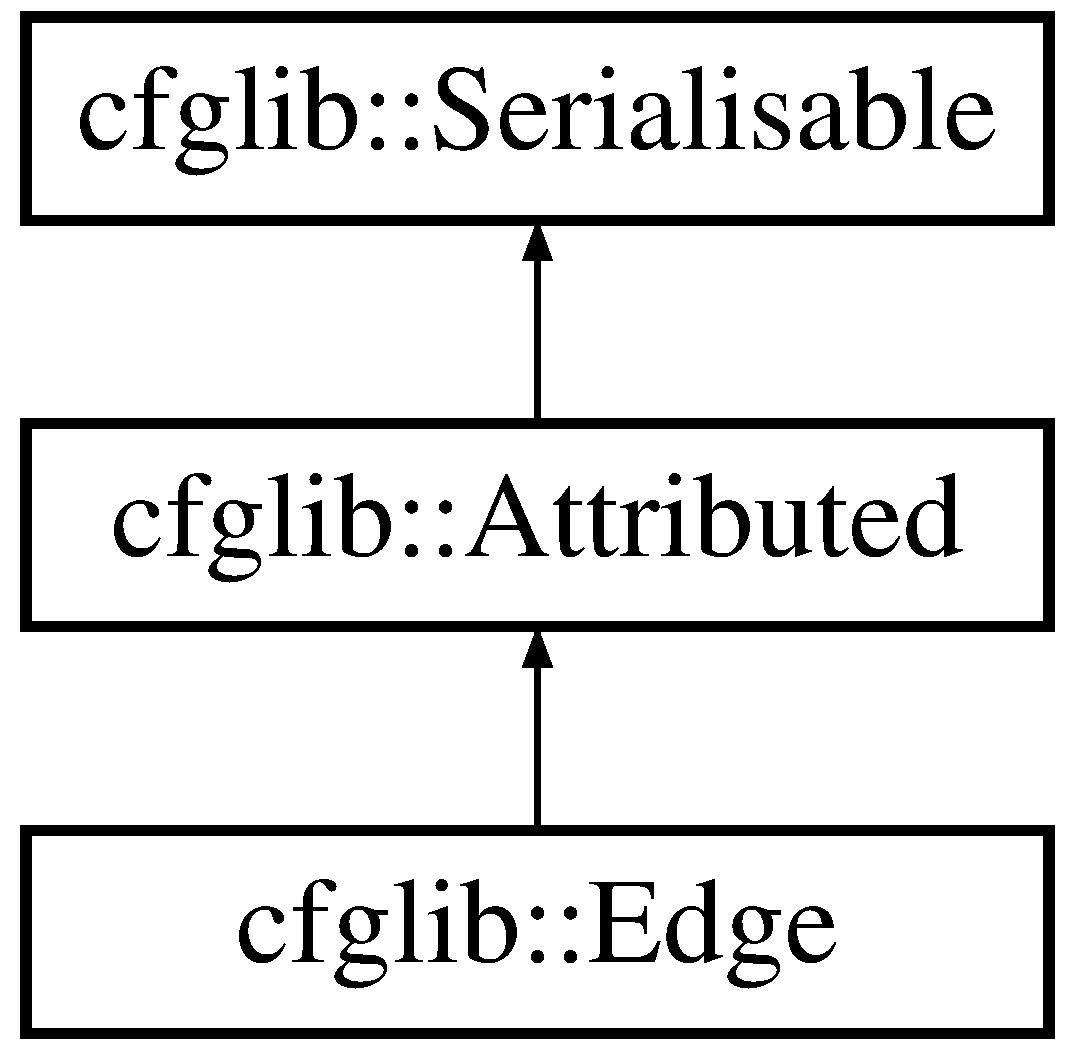
\includegraphics[height=3.000000cm]{classcfglib_1_1Edge}
\end{center}
\end{figure}
\subsection*{Public Member Functions}
\begin{DoxyCompactItemize}
\item 
\hyperlink{classcfglib_1_1Node}{Node} $\ast$ \hyperlink{classcfglib_1_1Edge_a217bd00a0276e3753ad8e34c2e57de44}{Get\+Source} ()
\item 
\hyperlink{classcfglib_1_1Node}{Node} $\ast$ \hyperlink{classcfglib_1_1Edge_ac5af20f98b5f5ceaad6383f1a953cc4e}{Get\+Target} ()
\item 
\hyperlink{classcfglib_1_1Edge}{Edge} $\ast$ \hyperlink{classcfglib_1_1Edge_a63c1a3697beb4b1734455c92d647f04c}{Clone} (\hyperlink{classcfglib_1_1CloneHandle}{Clone\+Handle} \&)
\item 
\hyperlink{classcfglib_1_1Cfg}{Cfg} $\ast$ \hyperlink{classcfglib_1_1Edge_ae1359932ba4c4d3e5e20c0391561e6a8}{Get\+Cfg} ()
\item 
virtual std\+::ostream \& \hyperlink{classcfglib_1_1Edge_af65bccb04bf1bad3f8a99d0b279836e0}{Write\+Xml} (std\+::ostream \&os, \hyperlink{classcfglib_1_1Handle}{Handle} \&hand)
\item 
virtual void \hyperlink{classcfglib_1_1Edge_af7eb95612c30e993771c519a2240cd77}{Read\+Xml} (\hyperlink{classXmlTag}{Xml\+Tag} const $\ast$tag, \hyperlink{classcfglib_1_1Handle}{Handle} \&handle)
\end{DoxyCompactItemize}
\subsection*{Friends}
\begin{DoxyCompactItemize}
\item 
class \hyperlink{classcfglib_1_1Edge_aad28e913031e836a51d46ca3a1a3b68b}{Cfg}
\item 
class \hyperlink{classcfglib_1_1Edge_a6f7095d721dd1dbd490d97c028eb676f}{Loop}
\end{DoxyCompactItemize}


\subsection{Detailed Description}
This class represents an \hyperlink{classcfglib_1_1Edge}{Edge}. T\+O\+DO\+: I do not know if this class implements yet the {\ttfamily \hyperlink{classcfglib_1_1Attributed}{Attributed}} interface. 

\subsection{Member Function Documentation}
\mbox{\Hypertarget{classcfglib_1_1Edge_a63c1a3697beb4b1734455c92d647f04c}\label{classcfglib_1_1Edge_a63c1a3697beb4b1734455c92d647f04c}} 
\index{cfglib\+::\+Edge@{cfglib\+::\+Edge}!Clone@{Clone}}
\index{Clone@{Clone}!cfglib\+::\+Edge@{cfglib\+::\+Edge}}
\subsubsection{\texorpdfstring{Clone()}{Clone()}}
{\footnotesize\ttfamily \hyperlink{classcfglib_1_1Edge}{Edge}$\ast$ cfglib\+::\+Edge\+::\+Clone (\begin{DoxyParamCaption}\item[{\hyperlink{classcfglib_1_1CloneHandle}{Clone\+Handle} \&}]{ }\end{DoxyParamCaption})}

cloning function \mbox{\Hypertarget{classcfglib_1_1Edge_ae1359932ba4c4d3e5e20c0391561e6a8}\label{classcfglib_1_1Edge_ae1359932ba4c4d3e5e20c0391561e6a8}} 
\index{cfglib\+::\+Edge@{cfglib\+::\+Edge}!Get\+Cfg@{Get\+Cfg}}
\index{Get\+Cfg@{Get\+Cfg}!cfglib\+::\+Edge@{cfglib\+::\+Edge}}
\subsubsection{\texorpdfstring{Get\+Cfg()}{GetCfg()}}
{\footnotesize\ttfamily \hyperlink{classcfglib_1_1Cfg}{Cfg}$\ast$ cfglib\+::\+Edge\+::\+Get\+Cfg (\begin{DoxyParamCaption}{ }\end{DoxyParamCaption})}

give the cfg of this \hyperlink{classcfglib_1_1Edge}{Edge}. \mbox{\Hypertarget{classcfglib_1_1Edge_a217bd00a0276e3753ad8e34c2e57de44}\label{classcfglib_1_1Edge_a217bd00a0276e3753ad8e34c2e57de44}} 
\index{cfglib\+::\+Edge@{cfglib\+::\+Edge}!Get\+Source@{Get\+Source}}
\index{Get\+Source@{Get\+Source}!cfglib\+::\+Edge@{cfglib\+::\+Edge}}
\subsubsection{\texorpdfstring{Get\+Source()}{GetSource()}}
{\footnotesize\ttfamily \hyperlink{classcfglib_1_1Node}{Node}$\ast$ cfglib\+::\+Edge\+::\+Get\+Source (\begin{DoxyParamCaption}{ }\end{DoxyParamCaption})}

return a pointer on the origin \hyperlink{classcfglib_1_1Node}{Node} . Internal helper function used by \hyperlink{classcfglib_1_1Cfg}{Cfg}. \mbox{\Hypertarget{classcfglib_1_1Edge_ac5af20f98b5f5ceaad6383f1a953cc4e}\label{classcfglib_1_1Edge_ac5af20f98b5f5ceaad6383f1a953cc4e}} 
\index{cfglib\+::\+Edge@{cfglib\+::\+Edge}!Get\+Target@{Get\+Target}}
\index{Get\+Target@{Get\+Target}!cfglib\+::\+Edge@{cfglib\+::\+Edge}}
\subsubsection{\texorpdfstring{Get\+Target()}{GetTarget()}}
{\footnotesize\ttfamily \hyperlink{classcfglib_1_1Node}{Node}$\ast$ cfglib\+::\+Edge\+::\+Get\+Target (\begin{DoxyParamCaption}{ }\end{DoxyParamCaption})}

return a pointer on the destination \hyperlink{classcfglib_1_1Node}{Node}. Internal helper function used by \hyperlink{classcfglib_1_1Cfg}{Cfg}. \mbox{\Hypertarget{classcfglib_1_1Edge_af7eb95612c30e993771c519a2240cd77}\label{classcfglib_1_1Edge_af7eb95612c30e993771c519a2240cd77}} 
\index{cfglib\+::\+Edge@{cfglib\+::\+Edge}!Read\+Xml@{Read\+Xml}}
\index{Read\+Xml@{Read\+Xml}!cfglib\+::\+Edge@{cfglib\+::\+Edge}}
\subsubsection{\texorpdfstring{Read\+Xml()}{ReadXml()}}
{\footnotesize\ttfamily virtual void cfglib\+::\+Edge\+::\+Read\+Xml (\begin{DoxyParamCaption}\item[{\hyperlink{classXmlTag}{Xml\+Tag} const $\ast$}]{tag,  }\item[{\hyperlink{classcfglib_1_1Handle}{Handle} \&}]{handle }\end{DoxyParamCaption})\hspace{0.3cm}{\ttfamily [virtual]}}

Deserialisation function.

The deserialisation is in two phase \+: first the creation of the object (in several ways depending on the object) and second call to O-\/$>$\hyperlink{classcfglib_1_1Edge_af7eb95612c30e993771c519a2240cd77}{Read\+Xml()} which initialize the object with correct values. 

Implements \hyperlink{classcfglib_1_1Serialisable_a876d530446317872259356af9b016e13}{cfglib\+::\+Serialisable}.

\mbox{\Hypertarget{classcfglib_1_1Edge_af65bccb04bf1bad3f8a99d0b279836e0}\label{classcfglib_1_1Edge_af65bccb04bf1bad3f8a99d0b279836e0}} 
\index{cfglib\+::\+Edge@{cfglib\+::\+Edge}!Write\+Xml@{Write\+Xml}}
\index{Write\+Xml@{Write\+Xml}!cfglib\+::\+Edge@{cfglib\+::\+Edge}}
\subsubsection{\texorpdfstring{Write\+Xml()}{WriteXml()}}
{\footnotesize\ttfamily virtual std\+::ostream\& cfglib\+::\+Edge\+::\+Write\+Xml (\begin{DoxyParamCaption}\item[{std\+::ostream \&}]{os,  }\item[{\hyperlink{classcfglib_1_1Handle}{Handle} \&}]{hand }\end{DoxyParamCaption})\hspace{0.3cm}{\ttfamily [virtual]}}

Serialisation function. 

Implements \hyperlink{classcfglib_1_1Serialisable_aaeb80cc7397ad312e5ae34f39412ce42}{cfglib\+::\+Serialisable}.



\subsection{Friends And Related Function Documentation}
\mbox{\Hypertarget{classcfglib_1_1Edge_aad28e913031e836a51d46ca3a1a3b68b}\label{classcfglib_1_1Edge_aad28e913031e836a51d46ca3a1a3b68b}} 
\index{cfglib\+::\+Edge@{cfglib\+::\+Edge}!Cfg@{Cfg}}
\index{Cfg@{Cfg}!cfglib\+::\+Edge@{cfglib\+::\+Edge}}
\subsubsection{\texorpdfstring{Cfg}{Cfg}}
{\footnotesize\ttfamily friend class \hyperlink{classcfglib_1_1Cfg}{Cfg}\hspace{0.3cm}{\ttfamily [friend]}}

\mbox{\Hypertarget{classcfglib_1_1Edge_a6f7095d721dd1dbd490d97c028eb676f}\label{classcfglib_1_1Edge_a6f7095d721dd1dbd490d97c028eb676f}} 
\index{cfglib\+::\+Edge@{cfglib\+::\+Edge}!Loop@{Loop}}
\index{Loop@{Loop}!cfglib\+::\+Edge@{cfglib\+::\+Edge}}
\subsubsection{\texorpdfstring{Loop}{Loop}}
{\footnotesize\ttfamily friend class \hyperlink{classcfglib_1_1Loop}{Loop}\hspace{0.3cm}{\ttfamily [friend]}}



The documentation for this class was generated from the following file\+:\begin{DoxyCompactItemize}
\item 
include/\hyperlink{Edge_8h}{Edge.\+h}\end{DoxyCompactItemize}

\hypertarget{classcfglib_1_1Handle}{}\section{cfglib\+:\+:Handle Class Reference}
\label{classcfglib_1_1Handle}\index{cfglib\+::\+Handle@{cfglib\+::\+Handle}}


{\ttfamily \#include $<$Handle.\+h$>$}

\subsection*{Public Member Functions}
\begin{DoxyCompactItemize}
\item 
\hyperlink{classcfglib_1_1Handle_a98f8601f6e1dd65a9f9ba0e29254c1ce}{Handle} ()
\item 
void \hyperlink{classcfglib_1_1Handle_ab8a43d033b2fe3a68aecf4dbee61dba2}{add\+I\+D\+\_\+handle} (std\+::string const \&id, \hyperlink{classcfglib_1_1Serialisable}{Serialisable} $\ast$$\ast$ptr)
\item 
void \hyperlink{classcfglib_1_1Handle_ad50bcb573b09ca46cccd3ac988a653d0}{add\+I\+D\+\_\+serialisable} (std\+::string const \&, \hyperlink{classcfglib_1_1Serialisable}{Serialisable} $\ast$)
\item 
std\+::string \hyperlink{classcfglib_1_1Handle_afdd041bbbaea61823ad61918ceaad330}{identify} (\hyperlink{classcfglib_1_1Serialisable}{Serialisable} const $\ast$obj)
\item 
void \hyperlink{classcfglib_1_1Handle_a8f524a2c4b97e7e3dda8aaa0d6dcd577}{resolve\+Handles} ()
\item 
std\+::string \hyperlink{classcfglib_1_1Handle_a90922bce066e04b5d46df9d29b641840}{get\+Id} (\hyperlink{classcfglib_1_1Serialisable}{Serialisable} const $\ast$obj)
\end{DoxyCompactItemize}


\subsection{Detailed Description}
this class manipulate unique identifier during unserisalisation 

\subsection{Constructor \& Destructor Documentation}
\mbox{\Hypertarget{classcfglib_1_1Handle_a98f8601f6e1dd65a9f9ba0e29254c1ce}\label{classcfglib_1_1Handle_a98f8601f6e1dd65a9f9ba0e29254c1ce}} 
\index{cfglib\+::\+Handle@{cfglib\+::\+Handle}!Handle@{Handle}}
\index{Handle@{Handle}!cfglib\+::\+Handle@{cfglib\+::\+Handle}}
\subsubsection{\texorpdfstring{Handle()}{Handle()}}
{\footnotesize\ttfamily cfglib\+::\+Handle\+::\+Handle (\begin{DoxyParamCaption}{ }\end{DoxyParamCaption})}



\subsection{Member Function Documentation}
\mbox{\Hypertarget{classcfglib_1_1Handle_ab8a43d033b2fe3a68aecf4dbee61dba2}\label{classcfglib_1_1Handle_ab8a43d033b2fe3a68aecf4dbee61dba2}} 
\index{cfglib\+::\+Handle@{cfglib\+::\+Handle}!add\+I\+D\+\_\+handle@{add\+I\+D\+\_\+handle}}
\index{add\+I\+D\+\_\+handle@{add\+I\+D\+\_\+handle}!cfglib\+::\+Handle@{cfglib\+::\+Handle}}
\subsubsection{\texorpdfstring{add\+I\+D\+\_\+handle()}{addID\_handle()}}
{\footnotesize\ttfamily void cfglib\+::\+Handle\+::add\+I\+D\+\_\+handle (\begin{DoxyParamCaption}\item[{std\+::string const \&}]{id,  }\item[{\hyperlink{classcfglib_1_1Serialisable}{Serialisable} $\ast$$\ast$}]{ptr }\end{DoxyParamCaption})}

Declare a new handle to a \hyperlink{classcfglib_1_1Serialisable}{Serialisable} object. Declared handles will be updated when the method \hyperlink{classcfglib_1_1Handle_a8f524a2c4b97e7e3dda8aaa0d6dcd577}{resolve\+Handles()} will be called. The first argument is a string id and the second is a pointer to the memory place of the handle Serialisable$\ast$ A\+T\+T\+E\+N\+T\+I\+ON \+: ptr must be use only with no ordered structure !!! \mbox{\Hypertarget{classcfglib_1_1Handle_ad50bcb573b09ca46cccd3ac988a653d0}\label{classcfglib_1_1Handle_ad50bcb573b09ca46cccd3ac988a653d0}} 
\index{cfglib\+::\+Handle@{cfglib\+::\+Handle}!add\+I\+D\+\_\+serialisable@{add\+I\+D\+\_\+serialisable}}
\index{add\+I\+D\+\_\+serialisable@{add\+I\+D\+\_\+serialisable}!cfglib\+::\+Handle@{cfglib\+::\+Handle}}
\subsubsection{\texorpdfstring{add\+I\+D\+\_\+serialisable()}{addID\_serialisable()}}
{\footnotesize\ttfamily void cfglib\+::\+Handle\+::add\+I\+D\+\_\+serialisable (\begin{DoxyParamCaption}\item[{std\+::string const \&}]{,  }\item[{\hyperlink{classcfglib_1_1Serialisable}{Serialisable} $\ast$}]{ }\end{DoxyParamCaption})}

Declare a \hyperlink{classcfglib_1_1Serialisable}{Serialisable} and its identifier. Objects are declared by the library, an also by library user. \mbox{\Hypertarget{classcfglib_1_1Handle_a90922bce066e04b5d46df9d29b641840}\label{classcfglib_1_1Handle_a90922bce066e04b5d46df9d29b641840}} 
\index{cfglib\+::\+Handle@{cfglib\+::\+Handle}!get\+Id@{get\+Id}}
\index{get\+Id@{get\+Id}!cfglib\+::\+Handle@{cfglib\+::\+Handle}}
\subsubsection{\texorpdfstring{get\+Id()}{getId()}}
{\footnotesize\ttfamily std\+::string cfglib\+::\+Handle\+::get\+Id (\begin{DoxyParamCaption}\item[{\hyperlink{classcfglib_1_1Serialisable}{Serialisable} const $\ast$}]{obj }\end{DoxyParamCaption})}

\mbox{\Hypertarget{classcfglib_1_1Handle_afdd041bbbaea61823ad61918ceaad330}\label{classcfglib_1_1Handle_afdd041bbbaea61823ad61918ceaad330}} 
\index{cfglib\+::\+Handle@{cfglib\+::\+Handle}!identify@{identify}}
\index{identify@{identify}!cfglib\+::\+Handle@{cfglib\+::\+Handle}}
\subsubsection{\texorpdfstring{identify()}{identify()}}
{\footnotesize\ttfamily std\+::string cfglib\+::\+Handle\+::identify (\begin{DoxyParamCaption}\item[{\hyperlink{classcfglib_1_1Serialisable}{Serialisable} const $\ast$}]{obj }\end{DoxyParamCaption})}

during serialisation give a unique identifier for each \hyperlink{classcfglib_1_1Serialisable}{Serialisable} object. Identity of objects is given by their address (you pass a pointer), be careful to not modify dynamic containers during serialisation. \mbox{\Hypertarget{classcfglib_1_1Handle_a8f524a2c4b97e7e3dda8aaa0d6dcd577}\label{classcfglib_1_1Handle_a8f524a2c4b97e7e3dda8aaa0d6dcd577}} 
\index{cfglib\+::\+Handle@{cfglib\+::\+Handle}!resolve\+Handles@{resolve\+Handles}}
\index{resolve\+Handles@{resolve\+Handles}!cfglib\+::\+Handle@{cfglib\+::\+Handle}}
\subsubsection{\texorpdfstring{resolve\+Handles()}{resolveHandles()}}
{\footnotesize\ttfamily void cfglib\+::\+Handle\+::resolve\+Handles (\begin{DoxyParamCaption}{ }\end{DoxyParamCaption})}

Replace all handles with their final value. not intended for library user, this function is used only by unserialisation predefined routine. 

The documentation for this class was generated from the following file\+:\begin{DoxyCompactItemize}
\item 
include/\hyperlink{Handle_8h}{Handle.\+h}\end{DoxyCompactItemize}

\hypertarget{classcfglib_1_1Instruction}{}\section{cfglib\+:\+:Instruction Class Reference}
\label{classcfglib_1_1Instruction}\index{cfglib\+::\+Instruction@{cfglib\+::\+Instruction}}


{\ttfamily \#include $<$Instruction.\+h$>$}

Inheritance diagram for cfglib\+:\+:Instruction\+:\begin{figure}[H]
\begin{center}
\leavevmode
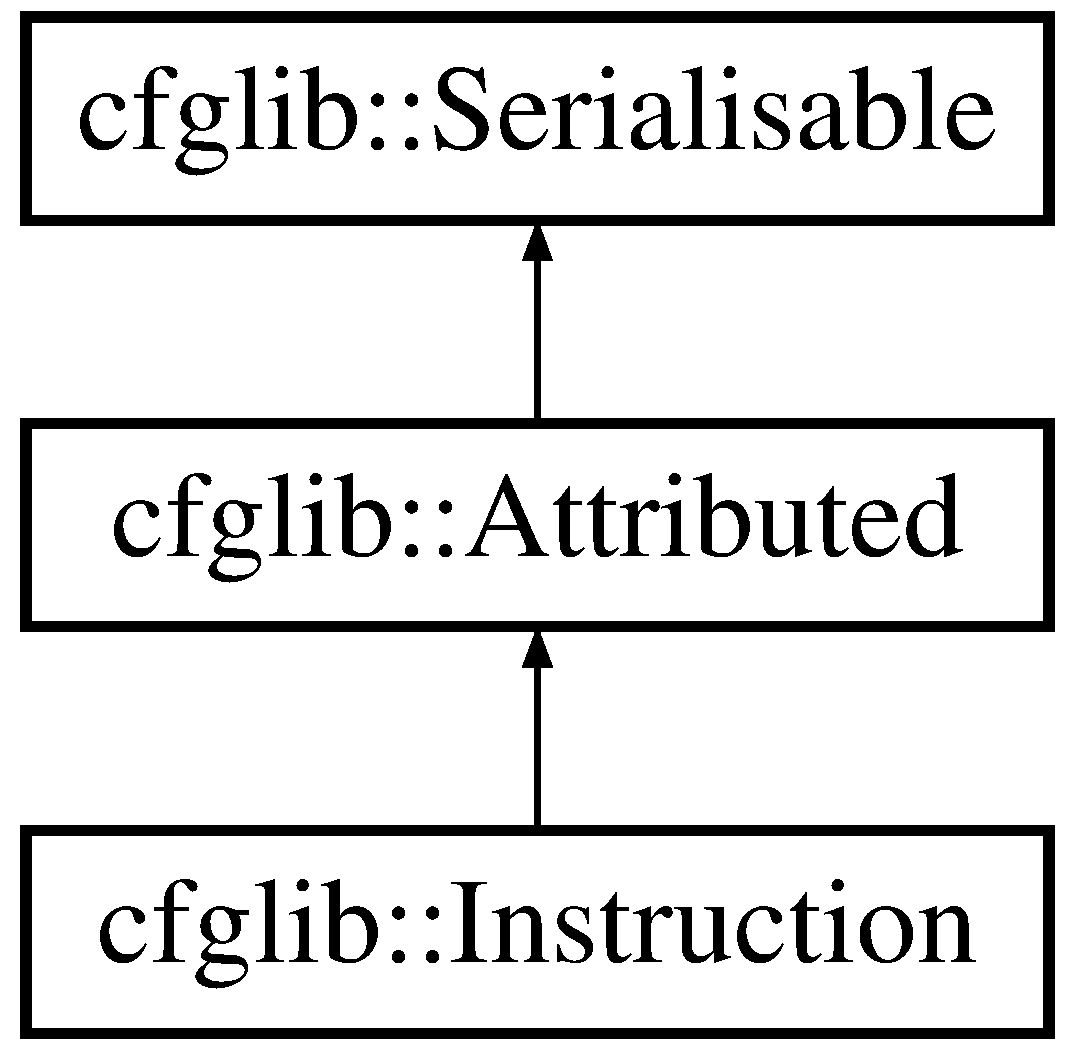
\includegraphics[height=3.000000cm]{classcfglib_1_1Instruction}
\end{center}
\end{figure}
\subsection*{Public Member Functions}
\begin{DoxyCompactItemize}
\item 
\hyperlink{classcfglib_1_1Instruction_afbca05ecb59e5a9b0b0027aadab48738}{Instruction} ()
\item 
\hyperlink{classcfglib_1_1Instruction_a22e42389cb62f96a0b28e3f7ebd1b323}{Instruction} (std\+::string const \&code, \hyperlink{namespacecfglib_a5ae32d51cf4ff1db5485367eab63a500}{asm\+\_\+type} type)
\item 
\hyperlink{classcfglib_1_1Instruction_aea2b37b89a6d029c20d0a49f1c89db66}{$\sim$\+Instruction} ()
\item 
\hyperlink{classcfglib_1_1Instruction}{Instruction} $\ast$ \hyperlink{classcfglib_1_1Instruction_a23db173ff853ab41327333fd8b87b61c}{Clone} ()
\item 
\hyperlink{classcfglib_1_1Instruction}{Instruction} $\ast$ \hyperlink{classcfglib_1_1Instruction_a32a5438b8eb037f9551518679e1c576a}{Clone} (\hyperlink{classcfglib_1_1CloneHandle}{Clone\+Handle} \&)
\item 
std\+::ostream \& \hyperlink{classcfglib_1_1Instruction_a1775270fdbf4f48e63d75c1327b51aa6}{Write\+Xml} (std\+::ostream \&os, \hyperlink{classcfglib_1_1Handle}{Handle} \&hand)
\item 
virtual void \hyperlink{classcfglib_1_1Instruction_a993641abc0297a715f66040d6ad7444c}{Read\+Xml} (\hyperlink{classXmlTag}{Xml\+Tag} const $\ast$tag, \hyperlink{classcfglib_1_1Handle}{Handle} \&hand)
\item 
std\+::string \hyperlink{classcfglib_1_1Instruction_a383f3ba3adf01b1596825b2314cdd5a9}{Get\+Code} ()
\item 
bool \hyperlink{classcfglib_1_1Instruction_accc89f23195a6da61676c34716e15527}{Is\+Code} ()
\item 
bool \hyperlink{classcfglib_1_1Instruction_aa0062264ffcc446ea706e15e3430543d}{Is\+Macro} ()
\item 
bool \hyperlink{classcfglib_1_1Instruction_a2611829fdb75f7be9545bbb2a0e0ff3f}{Is\+Directive} ()
\item 
bool \hyperlink{classcfglib_1_1Instruction_a28fda4549853eed5cb37e0330383b3bc}{Is\+Label} ()
\item 
bool \hyperlink{classcfglib_1_1Instruction_aff053b1bab7383efc4f563ad5b6b4c48}{Is\+Other} ()
\end{DoxyCompactItemize}


\subsection{Constructor \& Destructor Documentation}
\mbox{\Hypertarget{classcfglib_1_1Instruction_afbca05ecb59e5a9b0b0027aadab48738}\label{classcfglib_1_1Instruction_afbca05ecb59e5a9b0b0027aadab48738}} 
\index{cfglib\+::\+Instruction@{cfglib\+::\+Instruction}!Instruction@{Instruction}}
\index{Instruction@{Instruction}!cfglib\+::\+Instruction@{cfglib\+::\+Instruction}}
\subsubsection{\texorpdfstring{Instruction()}{Instruction()}\hspace{0.1cm}{\footnotesize\ttfamily [1/2]}}
{\footnotesize\ttfamily cfglib\+::\+Instruction\+::\+Instruction (\begin{DoxyParamCaption}{ }\end{DoxyParamCaption})}

Constructor \mbox{\Hypertarget{classcfglib_1_1Instruction_a22e42389cb62f96a0b28e3f7ebd1b323}\label{classcfglib_1_1Instruction_a22e42389cb62f96a0b28e3f7ebd1b323}} 
\index{cfglib\+::\+Instruction@{cfglib\+::\+Instruction}!Instruction@{Instruction}}
\index{Instruction@{Instruction}!cfglib\+::\+Instruction@{cfglib\+::\+Instruction}}
\subsubsection{\texorpdfstring{Instruction()}{Instruction()}\hspace{0.1cm}{\footnotesize\ttfamily [2/2]}}
{\footnotesize\ttfamily cfglib\+::\+Instruction\+::\+Instruction (\begin{DoxyParamCaption}\item[{std\+::string const \&}]{code,  }\item[{\hyperlink{namespacecfglib_a5ae32d51cf4ff1db5485367eab63a500}{asm\+\_\+type}}]{type }\end{DoxyParamCaption})}

Normal constructor \mbox{\Hypertarget{classcfglib_1_1Instruction_aea2b37b89a6d029c20d0a49f1c89db66}\label{classcfglib_1_1Instruction_aea2b37b89a6d029c20d0a49f1c89db66}} 
\index{cfglib\+::\+Instruction@{cfglib\+::\+Instruction}!````~Instruction@{$\sim$\+Instruction}}
\index{````~Instruction@{$\sim$\+Instruction}!cfglib\+::\+Instruction@{cfglib\+::\+Instruction}}
\subsubsection{\texorpdfstring{$\sim$\+Instruction()}{~Instruction()}}
{\footnotesize\ttfamily cfglib\+::\+Instruction\+::$\sim$\+Instruction (\begin{DoxyParamCaption}{ }\end{DoxyParamCaption})}

destructor 

\subsection{Member Function Documentation}
\mbox{\Hypertarget{classcfglib_1_1Instruction_a23db173ff853ab41327333fd8b87b61c}\label{classcfglib_1_1Instruction_a23db173ff853ab41327333fd8b87b61c}} 
\index{cfglib\+::\+Instruction@{cfglib\+::\+Instruction}!Clone@{Clone}}
\index{Clone@{Clone}!cfglib\+::\+Instruction@{cfglib\+::\+Instruction}}
\subsubsection{\texorpdfstring{Clone()}{Clone()}\hspace{0.1cm}{\footnotesize\ttfamily [1/2]}}
{\footnotesize\ttfamily \hyperlink{classcfglib_1_1Instruction}{Instruction}$\ast$ cfglib\+::\+Instruction\+::\+Clone (\begin{DoxyParamCaption}{ }\end{DoxyParamCaption})}

Cloning function \mbox{\Hypertarget{classcfglib_1_1Instruction_a32a5438b8eb037f9551518679e1c576a}\label{classcfglib_1_1Instruction_a32a5438b8eb037f9551518679e1c576a}} 
\index{cfglib\+::\+Instruction@{cfglib\+::\+Instruction}!Clone@{Clone}}
\index{Clone@{Clone}!cfglib\+::\+Instruction@{cfglib\+::\+Instruction}}
\subsubsection{\texorpdfstring{Clone()}{Clone()}\hspace{0.1cm}{\footnotesize\ttfamily [2/2]}}
{\footnotesize\ttfamily \hyperlink{classcfglib_1_1Instruction}{Instruction}$\ast$ cfglib\+::\+Instruction\+::\+Clone (\begin{DoxyParamCaption}\item[{\hyperlink{classcfglib_1_1CloneHandle}{Clone\+Handle} \&}]{ }\end{DoxyParamCaption})}

\mbox{\Hypertarget{classcfglib_1_1Instruction_a383f3ba3adf01b1596825b2314cdd5a9}\label{classcfglib_1_1Instruction_a383f3ba3adf01b1596825b2314cdd5a9}} 
\index{cfglib\+::\+Instruction@{cfglib\+::\+Instruction}!Get\+Code@{Get\+Code}}
\index{Get\+Code@{Get\+Code}!cfglib\+::\+Instruction@{cfglib\+::\+Instruction}}
\subsubsection{\texorpdfstring{Get\+Code()}{GetCode()}}
{\footnotesize\ttfamily std\+::string cfglib\+::\+Instruction\+::\+Get\+Code (\begin{DoxyParamCaption}{ }\end{DoxyParamCaption})}

get the assembly code line \mbox{\Hypertarget{classcfglib_1_1Instruction_accc89f23195a6da61676c34716e15527}\label{classcfglib_1_1Instruction_accc89f23195a6da61676c34716e15527}} 
\index{cfglib\+::\+Instruction@{cfglib\+::\+Instruction}!Is\+Code@{Is\+Code}}
\index{Is\+Code@{Is\+Code}!cfglib\+::\+Instruction@{cfglib\+::\+Instruction}}
\subsubsection{\texorpdfstring{Is\+Code()}{IsCode()}}
{\footnotesize\ttfamily bool cfglib\+::\+Instruction\+::\+Is\+Code (\begin{DoxyParamCaption}{ }\end{DoxyParamCaption})\hspace{0.3cm}{\ttfamily [inline]}}

Returns true if the line is a Code line \mbox{\Hypertarget{classcfglib_1_1Instruction_a2611829fdb75f7be9545bbb2a0e0ff3f}\label{classcfglib_1_1Instruction_a2611829fdb75f7be9545bbb2a0e0ff3f}} 
\index{cfglib\+::\+Instruction@{cfglib\+::\+Instruction}!Is\+Directive@{Is\+Directive}}
\index{Is\+Directive@{Is\+Directive}!cfglib\+::\+Instruction@{cfglib\+::\+Instruction}}
\subsubsection{\texorpdfstring{Is\+Directive()}{IsDirective()}}
{\footnotesize\ttfamily bool cfglib\+::\+Instruction\+::\+Is\+Directive (\begin{DoxyParamCaption}{ }\end{DoxyParamCaption})\hspace{0.3cm}{\ttfamily [inline]}}

Returns true if the line is a Directive \mbox{\Hypertarget{classcfglib_1_1Instruction_a28fda4549853eed5cb37e0330383b3bc}\label{classcfglib_1_1Instruction_a28fda4549853eed5cb37e0330383b3bc}} 
\index{cfglib\+::\+Instruction@{cfglib\+::\+Instruction}!Is\+Label@{Is\+Label}}
\index{Is\+Label@{Is\+Label}!cfglib\+::\+Instruction@{cfglib\+::\+Instruction}}
\subsubsection{\texorpdfstring{Is\+Label()}{IsLabel()}}
{\footnotesize\ttfamily bool cfglib\+::\+Instruction\+::\+Is\+Label (\begin{DoxyParamCaption}{ }\end{DoxyParamCaption})\hspace{0.3cm}{\ttfamily [inline]}}

Returns true if the line is a Labem \mbox{\Hypertarget{classcfglib_1_1Instruction_aa0062264ffcc446ea706e15e3430543d}\label{classcfglib_1_1Instruction_aa0062264ffcc446ea706e15e3430543d}} 
\index{cfglib\+::\+Instruction@{cfglib\+::\+Instruction}!Is\+Macro@{Is\+Macro}}
\index{Is\+Macro@{Is\+Macro}!cfglib\+::\+Instruction@{cfglib\+::\+Instruction}}
\subsubsection{\texorpdfstring{Is\+Macro()}{IsMacro()}}
{\footnotesize\ttfamily bool cfglib\+::\+Instruction\+::\+Is\+Macro (\begin{DoxyParamCaption}{ }\end{DoxyParamCaption})\hspace{0.3cm}{\ttfamily [inline]}}

Returns true if the line is a Macro line \mbox{\Hypertarget{classcfglib_1_1Instruction_aff053b1bab7383efc4f563ad5b6b4c48}\label{classcfglib_1_1Instruction_aff053b1bab7383efc4f563ad5b6b4c48}} 
\index{cfglib\+::\+Instruction@{cfglib\+::\+Instruction}!Is\+Other@{Is\+Other}}
\index{Is\+Other@{Is\+Other}!cfglib\+::\+Instruction@{cfglib\+::\+Instruction}}
\subsubsection{\texorpdfstring{Is\+Other()}{IsOther()}}
{\footnotesize\ttfamily bool cfglib\+::\+Instruction\+::\+Is\+Other (\begin{DoxyParamCaption}{ }\end{DoxyParamCaption})\hspace{0.3cm}{\ttfamily [inline]}}

Returns true if the line is an other type of line (eg comment, empty line) \mbox{\Hypertarget{classcfglib_1_1Instruction_a993641abc0297a715f66040d6ad7444c}\label{classcfglib_1_1Instruction_a993641abc0297a715f66040d6ad7444c}} 
\index{cfglib\+::\+Instruction@{cfglib\+::\+Instruction}!Read\+Xml@{Read\+Xml}}
\index{Read\+Xml@{Read\+Xml}!cfglib\+::\+Instruction@{cfglib\+::\+Instruction}}
\subsubsection{\texorpdfstring{Read\+Xml()}{ReadXml()}}
{\footnotesize\ttfamily virtual void cfglib\+::\+Instruction\+::\+Read\+Xml (\begin{DoxyParamCaption}\item[{\hyperlink{classXmlTag}{Xml\+Tag} const $\ast$}]{tag,  }\item[{\hyperlink{classcfglib_1_1Handle}{Handle} \&}]{hand }\end{DoxyParamCaption})\hspace{0.3cm}{\ttfamily [virtual]}}

Unserialisation function 

Implements \hyperlink{classcfglib_1_1Serialisable_a876d530446317872259356af9b016e13}{cfglib\+::\+Serialisable}.

\mbox{\Hypertarget{classcfglib_1_1Instruction_a1775270fdbf4f48e63d75c1327b51aa6}\label{classcfglib_1_1Instruction_a1775270fdbf4f48e63d75c1327b51aa6}} 
\index{cfglib\+::\+Instruction@{cfglib\+::\+Instruction}!Write\+Xml@{Write\+Xml}}
\index{Write\+Xml@{Write\+Xml}!cfglib\+::\+Instruction@{cfglib\+::\+Instruction}}
\subsubsection{\texorpdfstring{Write\+Xml()}{WriteXml()}}
{\footnotesize\ttfamily std\+::ostream\& cfglib\+::\+Instruction\+::\+Write\+Xml (\begin{DoxyParamCaption}\item[{std\+::ostream \&}]{os,  }\item[{\hyperlink{classcfglib_1_1Handle}{Handle} \&}]{hand }\end{DoxyParamCaption})\hspace{0.3cm}{\ttfamily [virtual]}}

Serialisation function. 

Implements \hyperlink{classcfglib_1_1Serialisable_aaeb80cc7397ad312e5ae34f39412ce42}{cfglib\+::\+Serialisable}.



The documentation for this class was generated from the following file\+:\begin{DoxyCompactItemize}
\item 
include/\hyperlink{Instruction_8h}{Instruction.\+h}\end{DoxyCompactItemize}

\hypertarget{classcfglib_1_1Loop}{}\section{cfglib\+:\+:Loop Class Reference}
\label{classcfglib_1_1Loop}\index{cfglib\+::\+Loop@{cfglib\+::\+Loop}}


{\ttfamily \#include $<$Loop.\+h$>$}

Inheritance diagram for cfglib\+:\+:Loop\+:\begin{figure}[H]
\begin{center}
\leavevmode
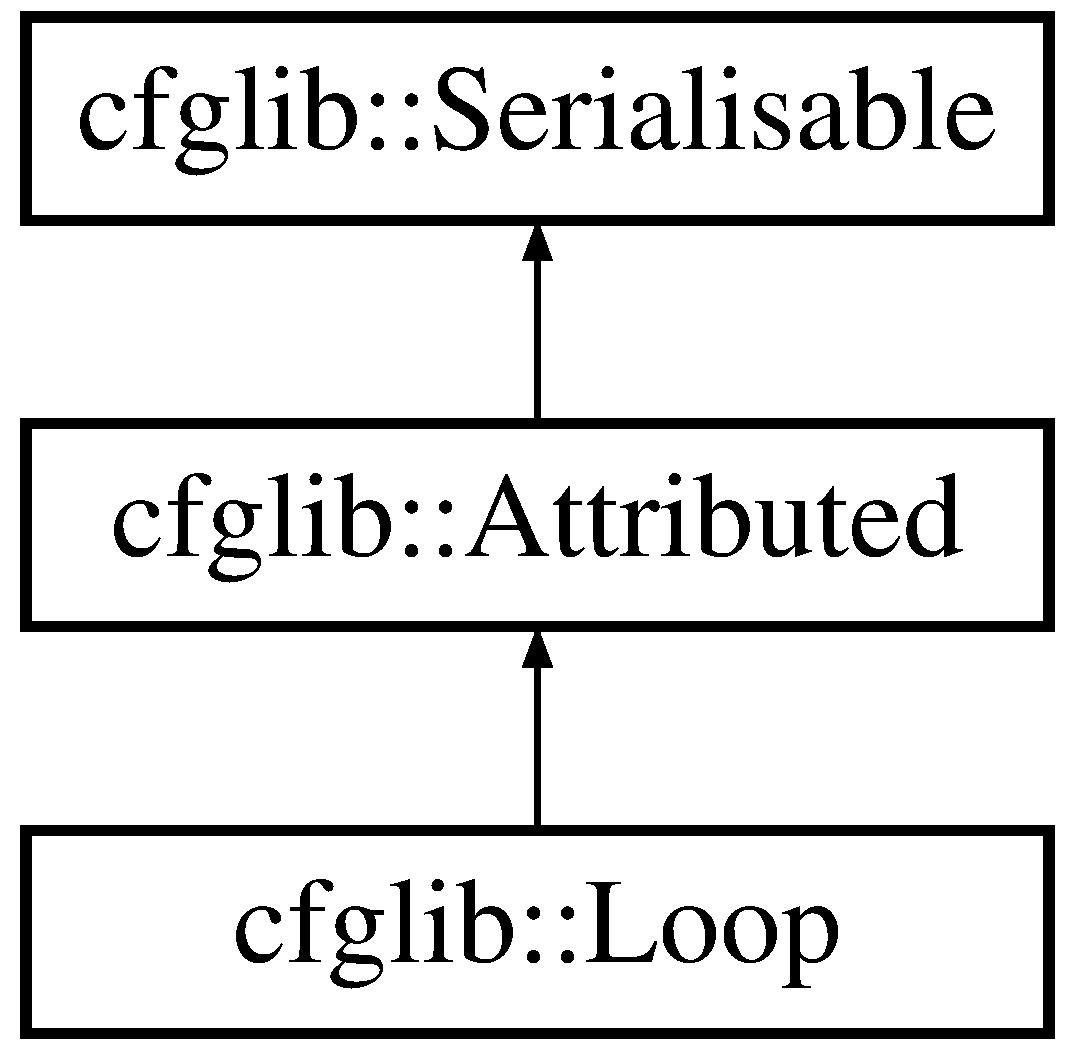
\includegraphics[height=3.000000cm]{classcfglib_1_1Loop}
\end{center}
\end{figure}
\subsection*{Public Member Functions}
\begin{DoxyCompactItemize}
\item 
\hyperlink{classcfglib_1_1Loop_a14d3e2db416417b9a0debad435307fb6}{Loop} ()
\item 
\hyperlink{classcfglib_1_1Loop_a7ce83c4b6b9fca7d2c4c86dfce6f4197}{$\sim$\+Loop} ()
\item 
\hyperlink{classcfglib_1_1Loop}{Loop} $\ast$ \hyperlink{classcfglib_1_1Loop_a87d6a91d0a7c1174e0c2ce2a205cb41e}{Clone} (\hyperlink{classcfglib_1_1CloneHandle}{Clone\+Handle} \&)
\item 
std\+::ostream \& \hyperlink{classcfglib_1_1Loop_a66cf343ede5add1036351ffd35d85065}{Write\+Xml} (std\+::ostream \&os, \hyperlink{classcfglib_1_1Handle}{Handle} \&hand)
\item 
virtual void \hyperlink{classcfglib_1_1Loop_a9bca6f0b552a7863259d34611dff7b4a}{Read\+Xml} (\hyperlink{classXmlTag}{Xml\+Tag} const $\ast$tag, \hyperlink{classcfglib_1_1Handle}{Handle} \&hand)
\item 
void \hyperlink{classcfglib_1_1Loop_ae6c9f22b961258f08b3f5e75629d0b1e}{Add\+Node} (\hyperlink{classcfglib_1_1Node}{Node} $\ast$)
\item 
void \hyperlink{classcfglib_1_1Loop_a2d327d15a95feaa19e09b83a1cf6a496}{Add\+Backedge} (\hyperlink{classcfglib_1_1Edge}{Edge} $\ast$)
\item 
\hyperlink{classcfglib_1_1Node}{Node} $\ast$ \hyperlink{classcfglib_1_1Loop_ae6a56b136cd76001c559b80172da3e64}{Get\+Head} () const
\item 
bool \hyperlink{classcfglib_1_1Loop_acbe30a927df0b77ed4aed07cb1517ba4}{Find\+In\+Loop} (\hyperlink{classcfglib_1_1Node}{Node} $\ast$node) const
\item 
std\+::vector$<$ \hyperlink{classcfglib_1_1Node}{Node} $\ast$ $>$ \hyperlink{classcfglib_1_1Loop_a20282571d9b3cef7723049480d3898fb}{Get\+All\+Nodes} () const
\item 
std\+::vector$<$ \hyperlink{classcfglib_1_1Node}{Node} $\ast$ $>$ \hyperlink{classcfglib_1_1Loop_a9dbb2c3b99d8a5cb6a89f725ac5e46b3}{Get\+All\+Nodes\+Not\+Nested} () const
\item 
std\+::vector$<$ \hyperlink{classcfglib_1_1Edge}{Edge} $\ast$ $>$ \hyperlink{classcfglib_1_1Loop_ae7a81ef3af9e19ef9cf86e4d807e76eb}{Get\+Backedges} () const
\item 
bool \hyperlink{classcfglib_1_1Loop_a8deea5bb51a437e8417143e77ee435a7}{Is\+Nested\+In} (\hyperlink{classcfglib_1_1Loop}{Loop} $\ast$l) const
\item 
void \hyperlink{classcfglib_1_1Loop_a8df5fb64b7864ba46b405dd16385fb90}{Peel} ()
\end{DoxyCompactItemize}


\subsection{Detailed Description}
Natural loops. 

\subsection{Constructor \& Destructor Documentation}
\mbox{\Hypertarget{classcfglib_1_1Loop_a14d3e2db416417b9a0debad435307fb6}\label{classcfglib_1_1Loop_a14d3e2db416417b9a0debad435307fb6}} 
\index{cfglib\+::\+Loop@{cfglib\+::\+Loop}!Loop@{Loop}}
\index{Loop@{Loop}!cfglib\+::\+Loop@{cfglib\+::\+Loop}}
\subsubsection{\texorpdfstring{Loop()}{Loop()}}
{\footnotesize\ttfamily cfglib\+::\+Loop\+::\+Loop (\begin{DoxyParamCaption}{ }\end{DoxyParamCaption})}

Constructor \mbox{\Hypertarget{classcfglib_1_1Loop_a7ce83c4b6b9fca7d2c4c86dfce6f4197}\label{classcfglib_1_1Loop_a7ce83c4b6b9fca7d2c4c86dfce6f4197}} 
\index{cfglib\+::\+Loop@{cfglib\+::\+Loop}!````~Loop@{$\sim$\+Loop}}
\index{````~Loop@{$\sim$\+Loop}!cfglib\+::\+Loop@{cfglib\+::\+Loop}}
\subsubsection{\texorpdfstring{$\sim$\+Loop()}{~Loop()}}
{\footnotesize\ttfamily cfglib\+::\+Loop\+::$\sim$\+Loop (\begin{DoxyParamCaption}{ }\end{DoxyParamCaption})}

destructor 

\subsection{Member Function Documentation}
\mbox{\Hypertarget{classcfglib_1_1Loop_a2d327d15a95feaa19e09b83a1cf6a496}\label{classcfglib_1_1Loop_a2d327d15a95feaa19e09b83a1cf6a496}} 
\index{cfglib\+::\+Loop@{cfglib\+::\+Loop}!Add\+Backedge@{Add\+Backedge}}
\index{Add\+Backedge@{Add\+Backedge}!cfglib\+::\+Loop@{cfglib\+::\+Loop}}
\subsubsection{\texorpdfstring{Add\+Backedge()}{AddBackedge()}}
{\footnotesize\ttfamily void cfglib\+::\+Loop\+::\+Add\+Backedge (\begin{DoxyParamCaption}\item[{\hyperlink{classcfglib_1_1Edge}{Edge} $\ast$}]{ }\end{DoxyParamCaption})}

Add backedge to the loop. The Nodes of the backedge should be added independently. F\+I\+X\+ME\+: in the reductible loop case I could infer backedges from the head information and this function will be therefore redundant. \mbox{\Hypertarget{classcfglib_1_1Loop_ae6c9f22b961258f08b3f5e75629d0b1e}\label{classcfglib_1_1Loop_ae6c9f22b961258f08b3f5e75629d0b1e}} 
\index{cfglib\+::\+Loop@{cfglib\+::\+Loop}!Add\+Node@{Add\+Node}}
\index{Add\+Node@{Add\+Node}!cfglib\+::\+Loop@{cfglib\+::\+Loop}}
\subsubsection{\texorpdfstring{Add\+Node()}{AddNode()}}
{\footnotesize\ttfamily void cfglib\+::\+Loop\+::\+Add\+Node (\begin{DoxyParamCaption}\item[{\hyperlink{classcfglib_1_1Node}{Node} $\ast$}]{ }\end{DoxyParamCaption})}

Add nodes to the loop, the first \hyperlink{classcfglib_1_1Node}{Node} added must be the head of the loop \mbox{\Hypertarget{classcfglib_1_1Loop_a87d6a91d0a7c1174e0c2ce2a205cb41e}\label{classcfglib_1_1Loop_a87d6a91d0a7c1174e0c2ce2a205cb41e}} 
\index{cfglib\+::\+Loop@{cfglib\+::\+Loop}!Clone@{Clone}}
\index{Clone@{Clone}!cfglib\+::\+Loop@{cfglib\+::\+Loop}}
\subsubsection{\texorpdfstring{Clone()}{Clone()}}
{\footnotesize\ttfamily \hyperlink{classcfglib_1_1Loop}{Loop}$\ast$ cfglib\+::\+Loop\+::\+Clone (\begin{DoxyParamCaption}\item[{\hyperlink{classcfglib_1_1CloneHandle}{Clone\+Handle} \&}]{ }\end{DoxyParamCaption})}

cloning function \mbox{\Hypertarget{classcfglib_1_1Loop_acbe30a927df0b77ed4aed07cb1517ba4}\label{classcfglib_1_1Loop_acbe30a927df0b77ed4aed07cb1517ba4}} 
\index{cfglib\+::\+Loop@{cfglib\+::\+Loop}!Find\+In\+Loop@{Find\+In\+Loop}}
\index{Find\+In\+Loop@{Find\+In\+Loop}!cfglib\+::\+Loop@{cfglib\+::\+Loop}}
\subsubsection{\texorpdfstring{Find\+In\+Loop()}{FindInLoop()}}
{\footnotesize\ttfamily bool cfglib\+::\+Loop\+::\+Find\+In\+Loop (\begin{DoxyParamCaption}\item[{\hyperlink{classcfglib_1_1Node}{Node} $\ast$}]{node }\end{DoxyParamCaption}) const}

Say if the node is in this loop. \mbox{\Hypertarget{classcfglib_1_1Loop_a20282571d9b3cef7723049480d3898fb}\label{classcfglib_1_1Loop_a20282571d9b3cef7723049480d3898fb}} 
\index{cfglib\+::\+Loop@{cfglib\+::\+Loop}!Get\+All\+Nodes@{Get\+All\+Nodes}}
\index{Get\+All\+Nodes@{Get\+All\+Nodes}!cfglib\+::\+Loop@{cfglib\+::\+Loop}}
\subsubsection{\texorpdfstring{Get\+All\+Nodes()}{GetAllNodes()}}
{\footnotesize\ttfamily std\+::vector$<$\hyperlink{classcfglib_1_1Node}{Node}$\ast$$>$ cfglib\+::\+Loop\+::\+Get\+All\+Nodes (\begin{DoxyParamCaption}{ }\end{DoxyParamCaption}) const}

Get the nodes of the \hyperlink{classcfglib_1_1Loop}{Loop}. The vector\textquotesingle{}s first \hyperlink{classcfglib_1_1Node}{Node} is the head of the loop, other nodes are in no particular order. Returns all nodes of the loop, even those belonging to nested loops. To have only the nodes not belonging to nested loops, call method Get\+All\+Nodes\+Not\+Nested \mbox{\Hypertarget{classcfglib_1_1Loop_a9dbb2c3b99d8a5cb6a89f725ac5e46b3}\label{classcfglib_1_1Loop_a9dbb2c3b99d8a5cb6a89f725ac5e46b3}} 
\index{cfglib\+::\+Loop@{cfglib\+::\+Loop}!Get\+All\+Nodes\+Not\+Nested@{Get\+All\+Nodes\+Not\+Nested}}
\index{Get\+All\+Nodes\+Not\+Nested@{Get\+All\+Nodes\+Not\+Nested}!cfglib\+::\+Loop@{cfglib\+::\+Loop}}
\subsubsection{\texorpdfstring{Get\+All\+Nodes\+Not\+Nested()}{GetAllNodesNotNested()}}
{\footnotesize\ttfamily std\+::vector$<$\hyperlink{classcfglib_1_1Node}{Node}$\ast$$>$ cfglib\+::\+Loop\+::\+Get\+All\+Nodes\+Not\+Nested (\begin{DoxyParamCaption}{ }\end{DoxyParamCaption}) const}

Get the nodes of the \hyperlink{classcfglib_1_1Loop}{Loop}. The vector\textquotesingle{}s first \hyperlink{classcfglib_1_1Node}{Node} is the head of the loop, other nodes are in no particular order. Returns only the nodes not belonging to nested loops. To have all nodes, call method Get\+All\+Nodes \mbox{\Hypertarget{classcfglib_1_1Loop_ae7a81ef3af9e19ef9cf86e4d807e76eb}\label{classcfglib_1_1Loop_ae7a81ef3af9e19ef9cf86e4d807e76eb}} 
\index{cfglib\+::\+Loop@{cfglib\+::\+Loop}!Get\+Backedges@{Get\+Backedges}}
\index{Get\+Backedges@{Get\+Backedges}!cfglib\+::\+Loop@{cfglib\+::\+Loop}}
\subsubsection{\texorpdfstring{Get\+Backedges()}{GetBackedges()}}
{\footnotesize\ttfamily std\+::vector$<$\hyperlink{classcfglib_1_1Edge}{Edge}$\ast$$>$ cfglib\+::\+Loop\+::\+Get\+Backedges (\begin{DoxyParamCaption}{ }\end{DoxyParamCaption}) const}

Get the \hyperlink{classcfglib_1_1Loop}{Loop} Backedges. \mbox{\Hypertarget{classcfglib_1_1Loop_ae6a56b136cd76001c559b80172da3e64}\label{classcfglib_1_1Loop_ae6a56b136cd76001c559b80172da3e64}} 
\index{cfglib\+::\+Loop@{cfglib\+::\+Loop}!Get\+Head@{Get\+Head}}
\index{Get\+Head@{Get\+Head}!cfglib\+::\+Loop@{cfglib\+::\+Loop}}
\subsubsection{\texorpdfstring{Get\+Head()}{GetHead()}}
{\footnotesize\ttfamily \hyperlink{classcfglib_1_1Node}{Node}$\ast$ cfglib\+::\+Loop\+::\+Get\+Head (\begin{DoxyParamCaption}{ }\end{DoxyParamCaption}) const}

Get the entry node of the loop \mbox{\Hypertarget{classcfglib_1_1Loop_a8deea5bb51a437e8417143e77ee435a7}\label{classcfglib_1_1Loop_a8deea5bb51a437e8417143e77ee435a7}} 
\index{cfglib\+::\+Loop@{cfglib\+::\+Loop}!Is\+Nested\+In@{Is\+Nested\+In}}
\index{Is\+Nested\+In@{Is\+Nested\+In}!cfglib\+::\+Loop@{cfglib\+::\+Loop}}
\subsubsection{\texorpdfstring{Is\+Nested\+In()}{IsNestedIn()}}
{\footnotesize\ttfamily bool cfglib\+::\+Loop\+::\+Is\+Nested\+In (\begin{DoxyParamCaption}\item[{\hyperlink{classcfglib_1_1Loop}{Loop} $\ast$}]{l }\end{DoxyParamCaption}) const}

Returns true if the loop (this) is nested in loop (l) \mbox{\Hypertarget{classcfglib_1_1Loop_a8df5fb64b7864ba46b405dd16385fb90}\label{classcfglib_1_1Loop_a8df5fb64b7864ba46b405dd16385fb90}} 
\index{cfglib\+::\+Loop@{cfglib\+::\+Loop}!Peel@{Peel}}
\index{Peel@{Peel}!cfglib\+::\+Loop@{cfglib\+::\+Loop}}
\subsubsection{\texorpdfstring{Peel()}{Peel()}}
{\footnotesize\ttfamily void cfglib\+::\+Loop\+::\+Peel (\begin{DoxyParamCaption}{ }\end{DoxyParamCaption})}

\mbox{\Hypertarget{classcfglib_1_1Loop_a9bca6f0b552a7863259d34611dff7b4a}\label{classcfglib_1_1Loop_a9bca6f0b552a7863259d34611dff7b4a}} 
\index{cfglib\+::\+Loop@{cfglib\+::\+Loop}!Read\+Xml@{Read\+Xml}}
\index{Read\+Xml@{Read\+Xml}!cfglib\+::\+Loop@{cfglib\+::\+Loop}}
\subsubsection{\texorpdfstring{Read\+Xml()}{ReadXml()}}
{\footnotesize\ttfamily virtual void cfglib\+::\+Loop\+::\+Read\+Xml (\begin{DoxyParamCaption}\item[{\hyperlink{classXmlTag}{Xml\+Tag} const $\ast$}]{tag,  }\item[{\hyperlink{classcfglib_1_1Handle}{Handle} \&}]{hand }\end{DoxyParamCaption})\hspace{0.3cm}{\ttfamily [virtual]}}

Deserialisation function. 

Implements \hyperlink{classcfglib_1_1Serialisable_a876d530446317872259356af9b016e13}{cfglib\+::\+Serialisable}.

\mbox{\Hypertarget{classcfglib_1_1Loop_a66cf343ede5add1036351ffd35d85065}\label{classcfglib_1_1Loop_a66cf343ede5add1036351ffd35d85065}} 
\index{cfglib\+::\+Loop@{cfglib\+::\+Loop}!Write\+Xml@{Write\+Xml}}
\index{Write\+Xml@{Write\+Xml}!cfglib\+::\+Loop@{cfglib\+::\+Loop}}
\subsubsection{\texorpdfstring{Write\+Xml()}{WriteXml()}}
{\footnotesize\ttfamily std\+::ostream\& cfglib\+::\+Loop\+::\+Write\+Xml (\begin{DoxyParamCaption}\item[{std\+::ostream \&}]{os,  }\item[{\hyperlink{classcfglib_1_1Handle}{Handle} \&}]{hand }\end{DoxyParamCaption})\hspace{0.3cm}{\ttfamily [virtual]}}

Serialisation function. 

Implements \hyperlink{classcfglib_1_1Serialisable_aaeb80cc7397ad312e5ae34f39412ce42}{cfglib\+::\+Serialisable}.



The documentation for this class was generated from the following file\+:\begin{DoxyCompactItemize}
\item 
include/\hyperlink{Loop_8h}{Loop.\+h}\end{DoxyCompactItemize}

\hypertarget{classcfglib_1_1Node}{}\section{cfglib\+:\+:Node Class Reference}
\label{classcfglib_1_1Node}\index{cfglib\+::\+Node@{cfglib\+::\+Node}}


{\ttfamily \#include $<$Node.\+h$>$}

Inheritance diagram for cfglib\+:\+:Node\+:\begin{figure}[H]
\begin{center}
\leavevmode
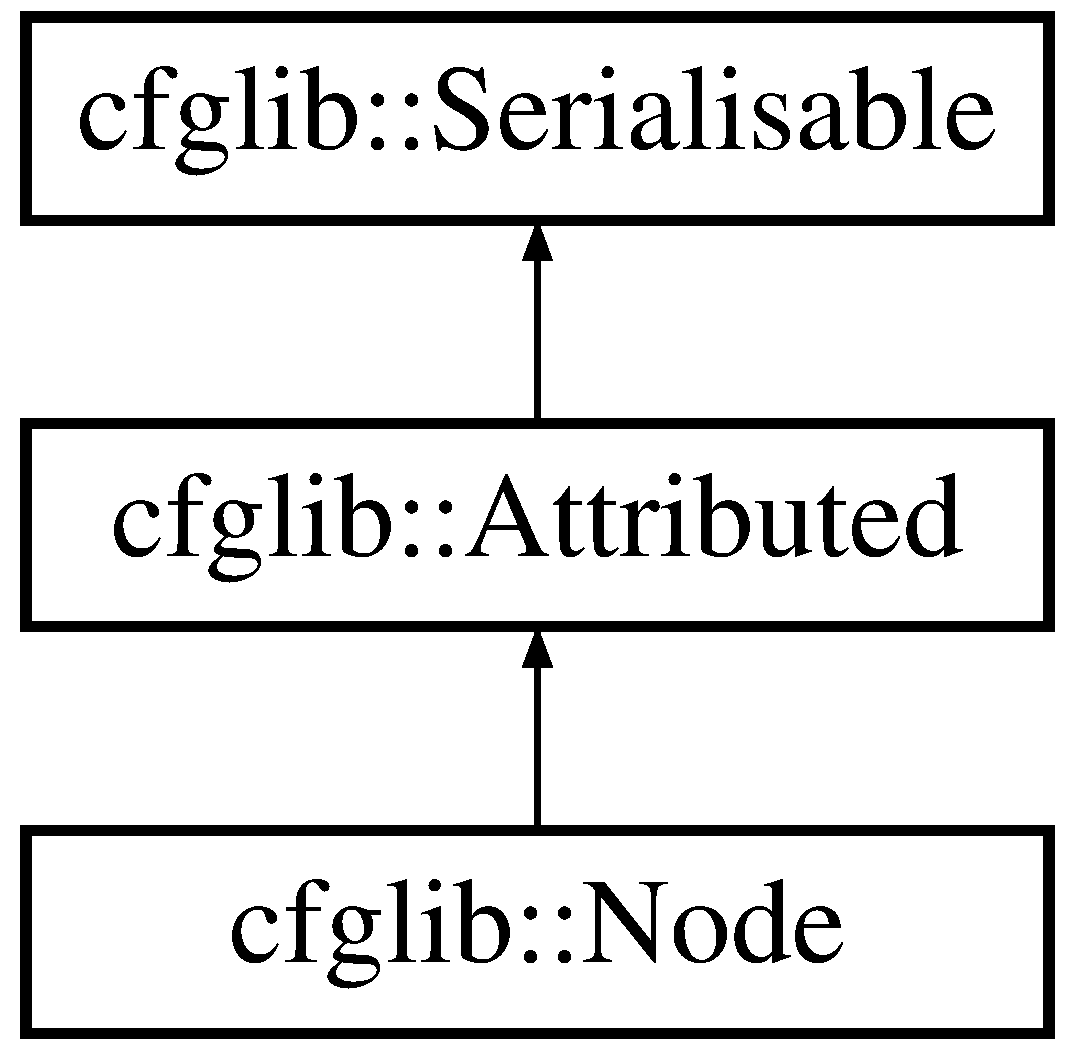
\includegraphics[height=3.000000cm]{classcfglib_1_1Node}
\end{center}
\end{figure}
\subsection*{Public Member Functions}
\begin{DoxyCompactItemize}
\item 
\hyperlink{classcfglib_1_1Cfg}{Cfg} $\ast$ \hyperlink{classcfglib_1_1Node_aba4169d7a66bceb6b5ae4e62193f669d}{Get\+Cfg} ()
\item 
virtual \hyperlink{classcfglib_1_1Node_a3ff420dfcc34125601765f1ab3444d66}{$\sim$\+Node} ()
\item 
\hyperlink{classcfglib_1_1Node}{Node} $\ast$ \hyperlink{classcfglib_1_1Node_a5f9b90a1d189124c775e0af9c209d208}{Clone} (\hyperlink{classcfglib_1_1CloneHandle}{Clone\+Handle} \&)
\item 
virtual std\+::ostream \& \hyperlink{classcfglib_1_1Node_a648aaa3e2703c9b5932bc50ffb14942c}{Write\+Xml} (std\+::ostream \&os, \hyperlink{classcfglib_1_1Handle}{Handle} \&hand)
\item 
virtual void \hyperlink{classcfglib_1_1Node_aaab769075e5d02c61411d58fc94e2070}{Read\+Xml} (\hyperlink{classXmlTag}{Xml\+Tag} const $\ast$tag, \hyperlink{classcfglib_1_1Handle}{Handle} \&hand)
\item 
\hyperlink{namespacecfglib_a44952a45d827aaa271f7e7dac5bf7752}{node\+\_\+type} \hyperlink{classcfglib_1_1Node_a92716d47e55c6808c641ac2fab7e26e2}{Get\+Type} ()
\item 
bool \hyperlink{classcfglib_1_1Node_a544488e1ba481dae0d55f2b826ac84a9}{Is\+Call} ()
\item 
bool \hyperlink{classcfglib_1_1Node_a2813d33e1f4b848f6f14f2744cb17dfe}{Is\+BB} ()
\item 
std\+::vector$<$ \hyperlink{classcfglib_1_1Instruction}{Instruction} $\ast$ $>$ \hyperlink{classcfglib_1_1Node_ad7e384556d7ab828b5e95536063668ad}{Get\+Instructions} ()
\item 
int \hyperlink{classcfglib_1_1Node_a305a0c9ac27d6840536be1ccbcea29d3}{Get\+Nb\+Instructions} ()
\item 
std\+::vector$<$ \hyperlink{classcfglib_1_1Instruction}{Instruction} $\ast$ $>$ \hyperlink{classcfglib_1_1Node_a75ef37984de980ec3866b68eb23864ae}{Get\+Asm} ()
\item 
\hyperlink{classcfglib_1_1Instruction}{Instruction} $\ast$ \hyperlink{classcfglib_1_1Node_ae0dc5993e16a3b637522c02819703833}{Create\+New\+Instruction} (std\+::string const \&code, \hyperlink{namespacecfglib_a5ae32d51cf4ff1db5485367eab63a500}{asm\+\_\+type} \hyperlink{namespacecfglib_a5ae32d51cf4ff1db5485367eab63a500}{asm\+\_\+type}, bool ret)
\item 
bool \hyperlink{classcfglib_1_1Node_a879a88114917dcc1084aeab10bd83732}{Is\+Return} ()
\item 
\hyperlink{classcfglib_1_1Cfg}{Cfg} $\ast$ \hyperlink{classcfglib_1_1Node_af9e169489c3a49ea3e6ef95e6b24ac69}{Get\+Callee} ()
\item 
std\+::string \hyperlink{classcfglib_1_1Node_af50258a896a1960fe337ce9bfb4c038e}{Get\+Callee\+Name} ()
\item 
void \hyperlink{classcfglib_1_1Node_a1ffbf02ce392ebbed1e56f75c3bb268d}{Set\+Call} (string called, bool emit\+\_\+warning)
\item 
bool \hyperlink{classcfglib_1_1Node_a52c4537c5aac77699ab900b8b60a14eb}{is\+Isolated\+Nop\+Node} ()
\item 
bool \hyperlink{classcfglib_1_1Node_a9063f79cf7bf36717b23a71c4027142e}{is\+Isolated\+Nop\+Node\+LB} ()
\item 
string \hyperlink{classcfglib_1_1Node_a42c979a43fa0e2314076fbecd3993514}{get\+Identifier} ()
\end{DoxyCompactItemize}
\subsection*{Friends}
\begin{DoxyCompactItemize}
\item 
class \hyperlink{classcfglib_1_1Node_aad28e913031e836a51d46ca3a1a3b68b}{Cfg}
\item 
class \hyperlink{classcfglib_1_1Node_a6f7095d721dd1dbd490d97c028eb676f}{Loop}
\end{DoxyCompactItemize}


\subsection{Detailed Description}
This abstract class represents a \hyperlink{classcfglib_1_1Node}{Node}. Nodes are basic components of a C\+FG. Nodes can be of type {\ttfamily BB} or {\ttfamily Call} A {\ttfamily Call} node contains instructions including the call instruction. 

\subsection{Constructor \& Destructor Documentation}
\mbox{\Hypertarget{classcfglib_1_1Node_a3ff420dfcc34125601765f1ab3444d66}\label{classcfglib_1_1Node_a3ff420dfcc34125601765f1ab3444d66}} 
\index{cfglib\+::\+Node@{cfglib\+::\+Node}!````~Node@{$\sim$\+Node}}
\index{````~Node@{$\sim$\+Node}!cfglib\+::\+Node@{cfglib\+::\+Node}}
\subsubsection{\texorpdfstring{$\sim$\+Node()}{~Node()}}
{\footnotesize\ttfamily virtual cfglib\+::\+Node\+::$\sim$\+Node (\begin{DoxyParamCaption}{ }\end{DoxyParamCaption})\hspace{0.3cm}{\ttfamily [virtual]}}

basic destructor 

\subsection{Member Function Documentation}
\mbox{\Hypertarget{classcfglib_1_1Node_a5f9b90a1d189124c775e0af9c209d208}\label{classcfglib_1_1Node_a5f9b90a1d189124c775e0af9c209d208}} 
\index{cfglib\+::\+Node@{cfglib\+::\+Node}!Clone@{Clone}}
\index{Clone@{Clone}!cfglib\+::\+Node@{cfglib\+::\+Node}}
\subsubsection{\texorpdfstring{Clone()}{Clone()}}
{\footnotesize\ttfamily \hyperlink{classcfglib_1_1Node}{Node}$\ast$ cfglib\+::\+Node\+::\+Clone (\begin{DoxyParamCaption}\item[{\hyperlink{classcfglib_1_1CloneHandle}{Clone\+Handle} \&}]{ }\end{DoxyParamCaption})}

cloning function \mbox{\Hypertarget{classcfglib_1_1Node_ae0dc5993e16a3b637522c02819703833}\label{classcfglib_1_1Node_ae0dc5993e16a3b637522c02819703833}} 
\index{cfglib\+::\+Node@{cfglib\+::\+Node}!Create\+New\+Instruction@{Create\+New\+Instruction}}
\index{Create\+New\+Instruction@{Create\+New\+Instruction}!cfglib\+::\+Node@{cfglib\+::\+Node}}
\subsubsection{\texorpdfstring{Create\+New\+Instruction()}{CreateNewInstruction()}}
{\footnotesize\ttfamily \hyperlink{classcfglib_1_1Instruction}{Instruction}$\ast$ cfglib\+::\+Node\+::\+Create\+New\+Instruction (\begin{DoxyParamCaption}\item[{std\+::string const \&}]{code,  }\item[{\hyperlink{namespacecfglib_a5ae32d51cf4ff1db5485367eab63a500}{asm\+\_\+type}}]{asm\+\_\+type,  }\item[{bool}]{ret }\end{DoxyParamCaption})}

Create new instruction. \hyperlink{classcfglib_1_1Instruction}{Instruction} must be added in the same order than for execution. \mbox{\Hypertarget{classcfglib_1_1Node_a75ef37984de980ec3866b68eb23864ae}\label{classcfglib_1_1Node_a75ef37984de980ec3866b68eb23864ae}} 
\index{cfglib\+::\+Node@{cfglib\+::\+Node}!Get\+Asm@{Get\+Asm}}
\index{Get\+Asm@{Get\+Asm}!cfglib\+::\+Node@{cfglib\+::\+Node}}
\subsubsection{\texorpdfstring{Get\+Asm()}{GetAsm()}}
{\footnotesize\ttfamily std\+::vector$<$\hyperlink{classcfglib_1_1Instruction}{Instruction} $\ast$$>$ cfglib\+::\+Node\+::\+Get\+Asm (\begin{DoxyParamCaption}{ }\end{DoxyParamCaption})}

Return the list of Code instructions of the \hyperlink{classcfglib_1_1Node}{Node} \mbox{\Hypertarget{classcfglib_1_1Node_af9e169489c3a49ea3e6ef95e6b24ac69}\label{classcfglib_1_1Node_af9e169489c3a49ea3e6ef95e6b24ac69}} 
\index{cfglib\+::\+Node@{cfglib\+::\+Node}!Get\+Callee@{Get\+Callee}}
\index{Get\+Callee@{Get\+Callee}!cfglib\+::\+Node@{cfglib\+::\+Node}}
\subsubsection{\texorpdfstring{Get\+Callee()}{GetCallee()}}
{\footnotesize\ttfamily \hyperlink{classcfglib_1_1Cfg}{Cfg}$\ast$ cfglib\+::\+Node\+::\+Get\+Callee (\begin{DoxyParamCaption}{ }\end{DoxyParamCaption})}

Applies to node of type Call to know which function it calls. return 0 on error or if the \hyperlink{classcfglib_1_1Node}{Node} is not a Call. \mbox{\Hypertarget{classcfglib_1_1Node_af50258a896a1960fe337ce9bfb4c038e}\label{classcfglib_1_1Node_af50258a896a1960fe337ce9bfb4c038e}} 
\index{cfglib\+::\+Node@{cfglib\+::\+Node}!Get\+Callee\+Name@{Get\+Callee\+Name}}
\index{Get\+Callee\+Name@{Get\+Callee\+Name}!cfglib\+::\+Node@{cfglib\+::\+Node}}
\subsubsection{\texorpdfstring{Get\+Callee\+Name()}{GetCalleeName()}}
{\footnotesize\ttfamily std\+::string cfglib\+::\+Node\+::\+Get\+Callee\+Name (\begin{DoxyParamCaption}{ }\end{DoxyParamCaption})}

Returns the name of the callee of the node is a Call node. returns the empty string if the node is not a Call node \mbox{\Hypertarget{classcfglib_1_1Node_aba4169d7a66bceb6b5ae4e62193f669d}\label{classcfglib_1_1Node_aba4169d7a66bceb6b5ae4e62193f669d}} 
\index{cfglib\+::\+Node@{cfglib\+::\+Node}!Get\+Cfg@{Get\+Cfg}}
\index{Get\+Cfg@{Get\+Cfg}!cfglib\+::\+Node@{cfglib\+::\+Node}}
\subsubsection{\texorpdfstring{Get\+Cfg()}{GetCfg()}}
{\footnotesize\ttfamily \hyperlink{classcfglib_1_1Cfg}{Cfg}$\ast$ cfglib\+::\+Node\+::\+Get\+Cfg (\begin{DoxyParamCaption}{ }\end{DoxyParamCaption})}

Return the \hyperlink{classcfglib_1_1Cfg}{Cfg} this \hyperlink{classcfglib_1_1Node}{Node} belong to. \mbox{\Hypertarget{classcfglib_1_1Node_a42c979a43fa0e2314076fbecd3993514}\label{classcfglib_1_1Node_a42c979a43fa0e2314076fbecd3993514}} 
\index{cfglib\+::\+Node@{cfglib\+::\+Node}!get\+Identifier@{get\+Identifier}}
\index{get\+Identifier@{get\+Identifier}!cfglib\+::\+Node@{cfglib\+::\+Node}}
\subsubsection{\texorpdfstring{get\+Identifier()}{getIdentifier()}}
{\footnotesize\ttfamily string cfglib\+::\+Node\+::get\+Identifier (\begin{DoxyParamCaption}{ }\end{DoxyParamCaption})}

\mbox{\Hypertarget{classcfglib_1_1Node_ad7e384556d7ab828b5e95536063668ad}\label{classcfglib_1_1Node_ad7e384556d7ab828b5e95536063668ad}} 
\index{cfglib\+::\+Node@{cfglib\+::\+Node}!Get\+Instructions@{Get\+Instructions}}
\index{Get\+Instructions@{Get\+Instructions}!cfglib\+::\+Node@{cfglib\+::\+Node}}
\subsubsection{\texorpdfstring{Get\+Instructions()}{GetInstructions()}}
{\footnotesize\ttfamily std\+::vector$<$\hyperlink{classcfglib_1_1Instruction}{Instruction}$\ast$$>$ cfglib\+::\+Node\+::\+Get\+Instructions (\begin{DoxyParamCaption}{ }\end{DoxyParamCaption})}

Get instructions vector \mbox{\Hypertarget{classcfglib_1_1Node_a305a0c9ac27d6840536be1ccbcea29d3}\label{classcfglib_1_1Node_a305a0c9ac27d6840536be1ccbcea29d3}} 
\index{cfglib\+::\+Node@{cfglib\+::\+Node}!Get\+Nb\+Instructions@{Get\+Nb\+Instructions}}
\index{Get\+Nb\+Instructions@{Get\+Nb\+Instructions}!cfglib\+::\+Node@{cfglib\+::\+Node}}
\subsubsection{\texorpdfstring{Get\+Nb\+Instructions()}{GetNbInstructions()}}
{\footnotesize\ttfamily int cfglib\+::\+Node\+::\+Get\+Nb\+Instructions (\begin{DoxyParamCaption}{ }\end{DoxyParamCaption})\hspace{0.3cm}{\ttfamily [inline]}}

Get the number of asm lines (instructions + others) of the node \mbox{\Hypertarget{classcfglib_1_1Node_a92716d47e55c6808c641ac2fab7e26e2}\label{classcfglib_1_1Node_a92716d47e55c6808c641ac2fab7e26e2}} 
\index{cfglib\+::\+Node@{cfglib\+::\+Node}!Get\+Type@{Get\+Type}}
\index{Get\+Type@{Get\+Type}!cfglib\+::\+Node@{cfglib\+::\+Node}}
\subsubsection{\texorpdfstring{Get\+Type()}{GetType()}}
{\footnotesize\ttfamily \hyperlink{namespacecfglib_a44952a45d827aaa271f7e7dac5bf7752}{node\+\_\+type} cfglib\+::\+Node\+::\+Get\+Type (\begin{DoxyParamCaption}{ }\end{DoxyParamCaption})\hspace{0.3cm}{\ttfamily [inline]}}

Returns the node type \mbox{\Hypertarget{classcfglib_1_1Node_a2813d33e1f4b848f6f14f2744cb17dfe}\label{classcfglib_1_1Node_a2813d33e1f4b848f6f14f2744cb17dfe}} 
\index{cfglib\+::\+Node@{cfglib\+::\+Node}!Is\+BB@{Is\+BB}}
\index{Is\+BB@{Is\+BB}!cfglib\+::\+Node@{cfglib\+::\+Node}}
\subsubsection{\texorpdfstring{Is\+B\+B()}{IsBB()}}
{\footnotesize\ttfamily bool cfglib\+::\+Node\+::\+Is\+BB (\begin{DoxyParamCaption}{ }\end{DoxyParamCaption})}

Returns true if the node is a basic block \mbox{\Hypertarget{classcfglib_1_1Node_a544488e1ba481dae0d55f2b826ac84a9}\label{classcfglib_1_1Node_a544488e1ba481dae0d55f2b826ac84a9}} 
\index{cfglib\+::\+Node@{cfglib\+::\+Node}!Is\+Call@{Is\+Call}}
\index{Is\+Call@{Is\+Call}!cfglib\+::\+Node@{cfglib\+::\+Node}}
\subsubsection{\texorpdfstring{Is\+Call()}{IsCall()}}
{\footnotesize\ttfamily bool cfglib\+::\+Node\+::\+Is\+Call (\begin{DoxyParamCaption}{ }\end{DoxyParamCaption})}

Returns true if the node is a Call node \mbox{\Hypertarget{classcfglib_1_1Node_a52c4537c5aac77699ab900b8b60a14eb}\label{classcfglib_1_1Node_a52c4537c5aac77699ab900b8b60a14eb}} 
\index{cfglib\+::\+Node@{cfglib\+::\+Node}!is\+Isolated\+Nop\+Node@{is\+Isolated\+Nop\+Node}}
\index{is\+Isolated\+Nop\+Node@{is\+Isolated\+Nop\+Node}!cfglib\+::\+Node@{cfglib\+::\+Node}}
\subsubsection{\texorpdfstring{is\+Isolated\+Nop\+Node()}{isIsolatedNopNode()}}
{\footnotesize\ttfamily bool cfglib\+::\+Node\+::is\+Isolated\+Nop\+Node (\begin{DoxyParamCaption}{ }\end{DoxyParamCaption})}

\begin{DoxyReturn}{Returns}

\begin{DoxyItemize}
\item true if the node is composed of a instruction nop, and isolated (without pred/succ). In A\+RM, it is possible (there is no delay slot,but ....)
\item false totherwise. 
\end{DoxyItemize}
\end{DoxyReturn}
\mbox{\Hypertarget{classcfglib_1_1Node_a9063f79cf7bf36717b23a71c4027142e}\label{classcfglib_1_1Node_a9063f79cf7bf36717b23a71c4027142e}} 
\index{cfglib\+::\+Node@{cfglib\+::\+Node}!is\+Isolated\+Nop\+Node\+LB@{is\+Isolated\+Nop\+Node\+LB}}
\index{is\+Isolated\+Nop\+Node\+LB@{is\+Isolated\+Nop\+Node\+LB}!cfglib\+::\+Node@{cfglib\+::\+Node}}
\subsubsection{\texorpdfstring{is\+Isolated\+Nop\+Node\+L\+B()}{isIsolatedNopNodeLB()}}
{\footnotesize\ttfamily bool cfglib\+::\+Node\+::is\+Isolated\+Nop\+Node\+LB (\begin{DoxyParamCaption}{ }\end{DoxyParamCaption})}

\mbox{\Hypertarget{classcfglib_1_1Node_a879a88114917dcc1084aeab10bd83732}\label{classcfglib_1_1Node_a879a88114917dcc1084aeab10bd83732}} 
\index{cfglib\+::\+Node@{cfglib\+::\+Node}!Is\+Return@{Is\+Return}}
\index{Is\+Return@{Is\+Return}!cfglib\+::\+Node@{cfglib\+::\+Node}}
\subsubsection{\texorpdfstring{Is\+Return()}{IsReturn()}}
{\footnotesize\ttfamily bool cfglib\+::\+Node\+::\+Is\+Return (\begin{DoxyParamCaption}{ }\end{DoxyParamCaption})}

Return true if the BB ends with a return instruction. \mbox{\Hypertarget{classcfglib_1_1Node_aaab769075e5d02c61411d58fc94e2070}\label{classcfglib_1_1Node_aaab769075e5d02c61411d58fc94e2070}} 
\index{cfglib\+::\+Node@{cfglib\+::\+Node}!Read\+Xml@{Read\+Xml}}
\index{Read\+Xml@{Read\+Xml}!cfglib\+::\+Node@{cfglib\+::\+Node}}
\subsubsection{\texorpdfstring{Read\+Xml()}{ReadXml()}}
{\footnotesize\ttfamily virtual void cfglib\+::\+Node\+::\+Read\+Xml (\begin{DoxyParamCaption}\item[{\hyperlink{classXmlTag}{Xml\+Tag} const $\ast$}]{tag,  }\item[{\hyperlink{classcfglib_1_1Handle}{Handle} \&}]{hand }\end{DoxyParamCaption})\hspace{0.3cm}{\ttfamily [virtual]}}

Unserialisation 

Implements \hyperlink{classcfglib_1_1Serialisable_a876d530446317872259356af9b016e13}{cfglib\+::\+Serialisable}.

\mbox{\Hypertarget{classcfglib_1_1Node_a1ffbf02ce392ebbed1e56f75c3bb268d}\label{classcfglib_1_1Node_a1ffbf02ce392ebbed1e56f75c3bb268d}} 
\index{cfglib\+::\+Node@{cfglib\+::\+Node}!Set\+Call@{Set\+Call}}
\index{Set\+Call@{Set\+Call}!cfglib\+::\+Node@{cfglib\+::\+Node}}
\subsubsection{\texorpdfstring{Set\+Call()}{SetCall()}}
{\footnotesize\ttfamily void cfglib\+::\+Node\+::\+Set\+Call (\begin{DoxyParamCaption}\item[{string}]{called,  }\item[{bool}]{emit\+\_\+warning }\end{DoxyParamCaption})}

Set the node as a call node and update the required information. A warning message is printed on stderr if the called function has no \hyperlink{classcfglib_1_1Cfg}{Cfg}. When the called function does not have a \hyperlink{classcfglib_1_1Cfg}{Cfg}, regardless of the generation of a warning message, an empty \hyperlink{classcfglib_1_1Cfg}{Cfg} is generated. \mbox{\Hypertarget{classcfglib_1_1Node_a648aaa3e2703c9b5932bc50ffb14942c}\label{classcfglib_1_1Node_a648aaa3e2703c9b5932bc50ffb14942c}} 
\index{cfglib\+::\+Node@{cfglib\+::\+Node}!Write\+Xml@{Write\+Xml}}
\index{Write\+Xml@{Write\+Xml}!cfglib\+::\+Node@{cfglib\+::\+Node}}
\subsubsection{\texorpdfstring{Write\+Xml()}{WriteXml()}}
{\footnotesize\ttfamily virtual std\+::ostream\& cfglib\+::\+Node\+::\+Write\+Xml (\begin{DoxyParamCaption}\item[{std\+::ostream \&}]{os,  }\item[{\hyperlink{classcfglib_1_1Handle}{Handle} \&}]{hand }\end{DoxyParamCaption})\hspace{0.3cm}{\ttfamily [virtual]}}

Serialisation function. Implements the {\ttfamily \hyperlink{classcfglib_1_1Node}{Node}} interface. 

Implements \hyperlink{classcfglib_1_1Serialisable_aaeb80cc7397ad312e5ae34f39412ce42}{cfglib\+::\+Serialisable}.



\subsection{Friends And Related Function Documentation}
\mbox{\Hypertarget{classcfglib_1_1Node_aad28e913031e836a51d46ca3a1a3b68b}\label{classcfglib_1_1Node_aad28e913031e836a51d46ca3a1a3b68b}} 
\index{cfglib\+::\+Node@{cfglib\+::\+Node}!Cfg@{Cfg}}
\index{Cfg@{Cfg}!cfglib\+::\+Node@{cfglib\+::\+Node}}
\subsubsection{\texorpdfstring{Cfg}{Cfg}}
{\footnotesize\ttfamily friend class \hyperlink{classcfglib_1_1Cfg}{Cfg}\hspace{0.3cm}{\ttfamily [friend]}}

\hyperlink{classcfglib_1_1Cfg}{Cfg} can create Nodes, et caetera. \mbox{\Hypertarget{classcfglib_1_1Node_a6f7095d721dd1dbd490d97c028eb676f}\label{classcfglib_1_1Node_a6f7095d721dd1dbd490d97c028eb676f}} 
\index{cfglib\+::\+Node@{cfglib\+::\+Node}!Loop@{Loop}}
\index{Loop@{Loop}!cfglib\+::\+Node@{cfglib\+::\+Node}}
\subsubsection{\texorpdfstring{Loop}{Loop}}
{\footnotesize\ttfamily friend class \hyperlink{classcfglib_1_1Loop}{Loop}\hspace{0.3cm}{\ttfamily [friend]}}



The documentation for this class was generated from the following file\+:\begin{DoxyCompactItemize}
\item 
include/\hyperlink{Node_8h}{Node.\+h}\end{DoxyCompactItemize}

\hypertarget{classcfglib_1_1NonSerialisableAttribute}{}\section{cfglib\+:\+:Non\+Serialisable\+Attribute Class Reference}
\label{classcfglib_1_1NonSerialisableAttribute}\index{cfglib\+::\+Non\+Serialisable\+Attribute@{cfglib\+::\+Non\+Serialisable\+Attribute}}


{\ttfamily \#include $<$Non\+Serialisable\+Attributes.\+h$>$}

Inheritance diagram for cfglib\+:\+:Non\+Serialisable\+Attribute\+:\begin{figure}[H]
\begin{center}
\leavevmode
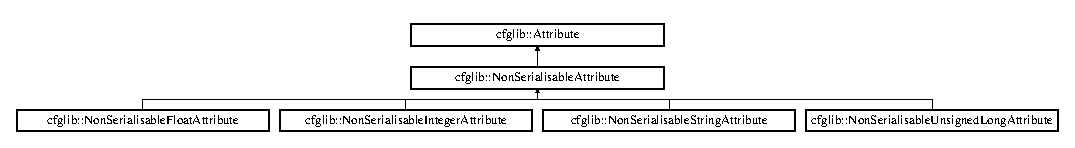
\includegraphics[height=1.538462cm]{classcfglib_1_1NonSerialisableAttribute}
\end{center}
\end{figure}
\subsection*{Additional Inherited Members}


\subsection{Detailed Description}
\hyperlink{classcfglib_1_1NonSerialisableAttribute}{Non\+Serialisable\+Attribute} are local attributes that are not expected to be serialised in X\+ML files. Ther are built-\/in \hyperlink{classcfglib_1_1NonSerialisableAttribute}{Non\+Serialisable\+Attribute} (integers, unisgned long, string, Big\+Integer). New non serialisable attributes can be defined by inheriting from class \hyperlink{classcfglib_1_1NonSerialisableAttribute}{Non\+Serialisable\+Attribute} 

The documentation for this class was generated from the following file\+:\begin{DoxyCompactItemize}
\item 
include/\hyperlink{NonSerialisableAttributes_8h}{Non\+Serialisable\+Attributes.\+h}\end{DoxyCompactItemize}

\hypertarget{classcfglib_1_1NonSerialisableFloatAttribute}{}\section{cfglib\+:\+:Non\+Serialisable\+Float\+Attribute Class Reference}
\label{classcfglib_1_1NonSerialisableFloatAttribute}\index{cfglib\+::\+Non\+Serialisable\+Float\+Attribute@{cfglib\+::\+Non\+Serialisable\+Float\+Attribute}}


{\ttfamily \#include $<$Non\+Serialisable\+Attributes.\+h$>$}

Inheritance diagram for cfglib\+:\+:Non\+Serialisable\+Float\+Attribute\+:\begin{figure}[H]
\begin{center}
\leavevmode
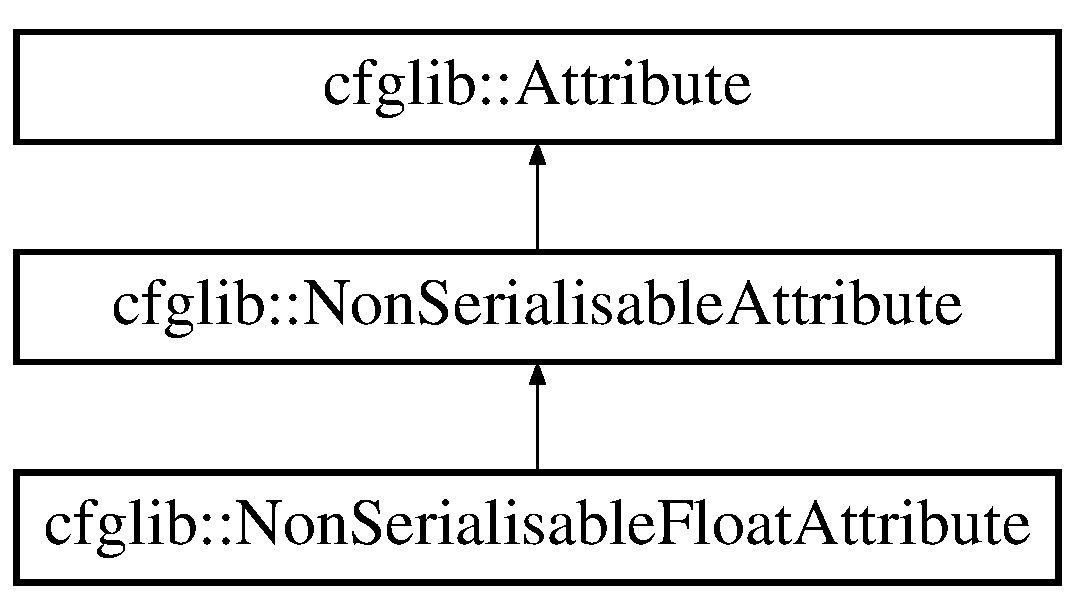
\includegraphics[height=3.000000cm]{classcfglib_1_1NonSerialisableFloatAttribute}
\end{center}
\end{figure}
\subsection*{Public Member Functions}
\begin{DoxyCompactItemize}
\item 
\hyperlink{classcfglib_1_1NonSerialisableFloatAttribute_a9f997d517dd321ec532c21c60a820d52}{Non\+Serialisable\+Float\+Attribute} (float val)
\item 
\hyperlink{classcfglib_1_1NonSerialisableFloatAttribute_a9dc9a9a6554ae4cb56337caba4db7ff8}{Non\+Serialisable\+Float\+Attribute} ()
\item 
virtual \hyperlink{classcfglib_1_1NonSerialisableFloatAttribute}{Non\+Serialisable\+Float\+Attribute} $\ast$ \hyperlink{classcfglib_1_1NonSerialisableFloatAttribute_a8cf8fa70d97d003cf48c64c59609eeaf}{clone} ()
\item 
void \hyperlink{classcfglib_1_1NonSerialisableFloatAttribute_a507fc8e93b9ff7c56d483f2e51634e67}{Print} (std\+::ostream \&s)
\item 
float \hyperlink{classcfglib_1_1NonSerialisableFloatAttribute_a4d2bc3d3ab44c4f8e05c6c0c6f3dfc4a}{Get\+Value} ()
\item 
void \hyperlink{classcfglib_1_1NonSerialisableFloatAttribute_a68b000967be65bfa02626352476ca64e}{Set\+Value} (float v)
\end{DoxyCompactItemize}
\subsection*{Additional Inherited Members}


\subsection{Detailed Description}
\hyperlink{classcfglib_1_1NonSerialisableFloatAttribute}{Non\+Serialisable\+Float\+Attribute} is a library-\/supported non serialisable attribute of type float 

\subsection{Constructor \& Destructor Documentation}
\mbox{\Hypertarget{classcfglib_1_1NonSerialisableFloatAttribute_a9f997d517dd321ec532c21c60a820d52}\label{classcfglib_1_1NonSerialisableFloatAttribute_a9f997d517dd321ec532c21c60a820d52}} 
\index{cfglib\+::\+Non\+Serialisable\+Float\+Attribute@{cfglib\+::\+Non\+Serialisable\+Float\+Attribute}!Non\+Serialisable\+Float\+Attribute@{Non\+Serialisable\+Float\+Attribute}}
\index{Non\+Serialisable\+Float\+Attribute@{Non\+Serialisable\+Float\+Attribute}!cfglib\+::\+Non\+Serialisable\+Float\+Attribute@{cfglib\+::\+Non\+Serialisable\+Float\+Attribute}}
\subsubsection{\texorpdfstring{Non\+Serialisable\+Float\+Attribute()}{NonSerialisableFloatAttribute()}\hspace{0.1cm}{\footnotesize\ttfamily [1/2]}}
{\footnotesize\ttfamily cfglib\+::\+Non\+Serialisable\+Float\+Attribute\+::\+Non\+Serialisable\+Float\+Attribute (\begin{DoxyParamCaption}\item[{float}]{val }\end{DoxyParamCaption})\hspace{0.3cm}{\ttfamily [inline]}}

Constructor \mbox{\Hypertarget{classcfglib_1_1NonSerialisableFloatAttribute_a9dc9a9a6554ae4cb56337caba4db7ff8}\label{classcfglib_1_1NonSerialisableFloatAttribute_a9dc9a9a6554ae4cb56337caba4db7ff8}} 
\index{cfglib\+::\+Non\+Serialisable\+Float\+Attribute@{cfglib\+::\+Non\+Serialisable\+Float\+Attribute}!Non\+Serialisable\+Float\+Attribute@{Non\+Serialisable\+Float\+Attribute}}
\index{Non\+Serialisable\+Float\+Attribute@{Non\+Serialisable\+Float\+Attribute}!cfglib\+::\+Non\+Serialisable\+Float\+Attribute@{cfglib\+::\+Non\+Serialisable\+Float\+Attribute}}
\subsubsection{\texorpdfstring{Non\+Serialisable\+Float\+Attribute()}{NonSerialisableFloatAttribute()}\hspace{0.1cm}{\footnotesize\ttfamily [2/2]}}
{\footnotesize\ttfamily cfglib\+::\+Non\+Serialisable\+Float\+Attribute\+::\+Non\+Serialisable\+Float\+Attribute (\begin{DoxyParamCaption}{ }\end{DoxyParamCaption})\hspace{0.3cm}{\ttfamily [inline]}}

default constructor. 

\subsection{Member Function Documentation}
\mbox{\Hypertarget{classcfglib_1_1NonSerialisableFloatAttribute_a8cf8fa70d97d003cf48c64c59609eeaf}\label{classcfglib_1_1NonSerialisableFloatAttribute_a8cf8fa70d97d003cf48c64c59609eeaf}} 
\index{cfglib\+::\+Non\+Serialisable\+Float\+Attribute@{cfglib\+::\+Non\+Serialisable\+Float\+Attribute}!clone@{clone}}
\index{clone@{clone}!cfglib\+::\+Non\+Serialisable\+Float\+Attribute@{cfglib\+::\+Non\+Serialisable\+Float\+Attribute}}
\subsubsection{\texorpdfstring{clone()}{clone()}}
{\footnotesize\ttfamily virtual \hyperlink{classcfglib_1_1NonSerialisableFloatAttribute}{Non\+Serialisable\+Float\+Attribute}$\ast$ cfglib\+::\+Non\+Serialisable\+Float\+Attribute\+::clone (\begin{DoxyParamCaption}{ }\end{DoxyParamCaption})\hspace{0.3cm}{\ttfamily [inline]}, {\ttfamily [virtual]}}

virtual constructor 

Implements \hyperlink{classcfglib_1_1Attribute_a107366042fdafe881215426059fec3f8}{cfglib\+::\+Attribute}.

\mbox{\Hypertarget{classcfglib_1_1NonSerialisableFloatAttribute_a4d2bc3d3ab44c4f8e05c6c0c6f3dfc4a}\label{classcfglib_1_1NonSerialisableFloatAttribute_a4d2bc3d3ab44c4f8e05c6c0c6f3dfc4a}} 
\index{cfglib\+::\+Non\+Serialisable\+Float\+Attribute@{cfglib\+::\+Non\+Serialisable\+Float\+Attribute}!Get\+Value@{Get\+Value}}
\index{Get\+Value@{Get\+Value}!cfglib\+::\+Non\+Serialisable\+Float\+Attribute@{cfglib\+::\+Non\+Serialisable\+Float\+Attribute}}
\subsubsection{\texorpdfstring{Get\+Value()}{GetValue()}}
{\footnotesize\ttfamily float cfglib\+::\+Non\+Serialisable\+Float\+Attribute\+::\+Get\+Value (\begin{DoxyParamCaption}{ }\end{DoxyParamCaption})\hspace{0.3cm}{\ttfamily [inline]}}

get int value of the Integer \hyperlink{classcfglib_1_1Attribute}{Attribute} \mbox{\Hypertarget{classcfglib_1_1NonSerialisableFloatAttribute_a507fc8e93b9ff7c56d483f2e51634e67}\label{classcfglib_1_1NonSerialisableFloatAttribute_a507fc8e93b9ff7c56d483f2e51634e67}} 
\index{cfglib\+::\+Non\+Serialisable\+Float\+Attribute@{cfglib\+::\+Non\+Serialisable\+Float\+Attribute}!Print@{Print}}
\index{Print@{Print}!cfglib\+::\+Non\+Serialisable\+Float\+Attribute@{cfglib\+::\+Non\+Serialisable\+Float\+Attribute}}
\subsubsection{\texorpdfstring{Print()}{Print()}}
{\footnotesize\ttfamily void cfglib\+::\+Non\+Serialisable\+Float\+Attribute\+::\+Print (\begin{DoxyParamCaption}\item[{std\+::ostream \&}]{s }\end{DoxyParamCaption})\hspace{0.3cm}{\ttfamily [inline]}, {\ttfamily [virtual]}}

\hyperlink{classcfglib_1_1Attribute}{Attribute} printing function (debug only) 

Implements \hyperlink{classcfglib_1_1Attribute_af8d87ceddde146b92727e61823e0129b}{cfglib\+::\+Attribute}.

\mbox{\Hypertarget{classcfglib_1_1NonSerialisableFloatAttribute_a68b000967be65bfa02626352476ca64e}\label{classcfglib_1_1NonSerialisableFloatAttribute_a68b000967be65bfa02626352476ca64e}} 
\index{cfglib\+::\+Non\+Serialisable\+Float\+Attribute@{cfglib\+::\+Non\+Serialisable\+Float\+Attribute}!Set\+Value@{Set\+Value}}
\index{Set\+Value@{Set\+Value}!cfglib\+::\+Non\+Serialisable\+Float\+Attribute@{cfglib\+::\+Non\+Serialisable\+Float\+Attribute}}
\subsubsection{\texorpdfstring{Set\+Value()}{SetValue()}}
{\footnotesize\ttfamily void cfglib\+::\+Non\+Serialisable\+Float\+Attribute\+::\+Set\+Value (\begin{DoxyParamCaption}\item[{float}]{v }\end{DoxyParamCaption})\hspace{0.3cm}{\ttfamily [inline]}}

set the value of the Integer attribute 

The documentation for this class was generated from the following file\+:\begin{DoxyCompactItemize}
\item 
include/\hyperlink{NonSerialisableAttributes_8h}{Non\+Serialisable\+Attributes.\+h}\end{DoxyCompactItemize}

\hypertarget{classcfglib_1_1NonSerialisableIntegerAttribute}{}\section{cfglib\+:\+:Non\+Serialisable\+Integer\+Attribute Class Reference}
\label{classcfglib_1_1NonSerialisableIntegerAttribute}\index{cfglib\+::\+Non\+Serialisable\+Integer\+Attribute@{cfglib\+::\+Non\+Serialisable\+Integer\+Attribute}}


{\ttfamily \#include $<$Non\+Serialisable\+Attributes.\+h$>$}

Inheritance diagram for cfglib\+:\+:Non\+Serialisable\+Integer\+Attribute\+:\begin{figure}[H]
\begin{center}
\leavevmode
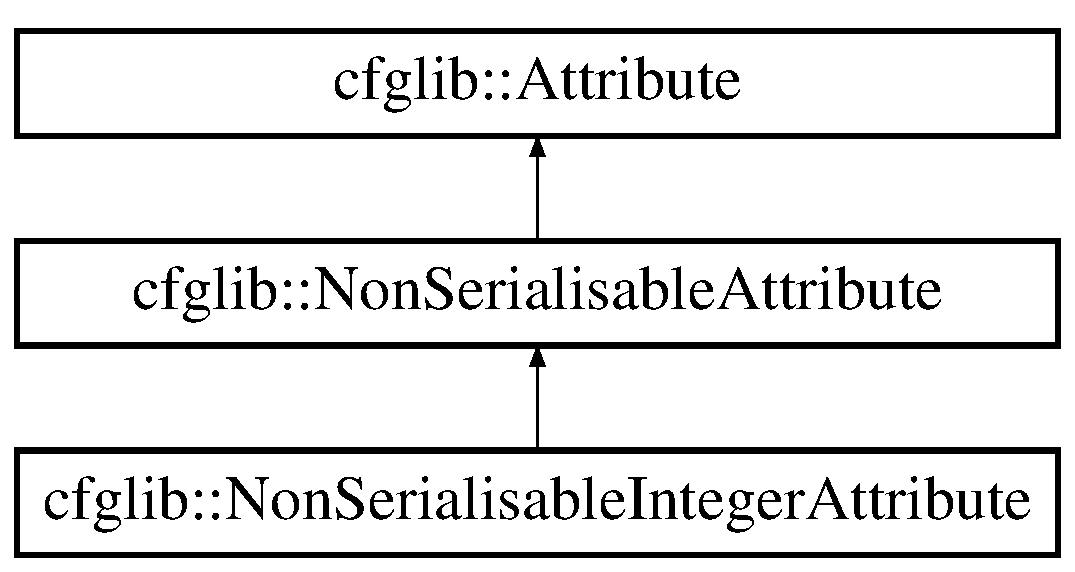
\includegraphics[height=3.000000cm]{classcfglib_1_1NonSerialisableIntegerAttribute}
\end{center}
\end{figure}
\subsection*{Public Member Functions}
\begin{DoxyCompactItemize}
\item 
\hyperlink{classcfglib_1_1NonSerialisableIntegerAttribute_a3500f80644bc62dcb3f4fcdaa47b5cc5}{Non\+Serialisable\+Integer\+Attribute} (int val)
\item 
\hyperlink{classcfglib_1_1NonSerialisableIntegerAttribute_a8242a4ef17361a5de82ed15130a78487}{Non\+Serialisable\+Integer\+Attribute} ()
\item 
virtual \hyperlink{classcfglib_1_1NonSerialisableIntegerAttribute}{Non\+Serialisable\+Integer\+Attribute} $\ast$ \hyperlink{classcfglib_1_1NonSerialisableIntegerAttribute_ab37d2f2a349d73177e6fdbd1356566ab}{clone} ()
\item 
void \hyperlink{classcfglib_1_1NonSerialisableIntegerAttribute_ade6c5738723b606295a2cf14fe568247}{Print} (std\+::ostream \&s)
\item 
int \hyperlink{classcfglib_1_1NonSerialisableIntegerAttribute_aeb200350a5746f7fe535ca4db1642e9d}{Get\+Value} ()
\item 
void \hyperlink{classcfglib_1_1NonSerialisableIntegerAttribute_a7bff73325941157e314046c31f266d2a}{Set\+Value} (int v)
\end{DoxyCompactItemize}
\subsection*{Additional Inherited Members}


\subsection{Detailed Description}
\hyperlink{classcfglib_1_1NonSerialisableIntegerAttribute}{Non\+Serialisable\+Integer\+Attribute} is a library-\/supported non serialisable attribute of type integer 

\subsection{Constructor \& Destructor Documentation}
\mbox{\Hypertarget{classcfglib_1_1NonSerialisableIntegerAttribute_a3500f80644bc62dcb3f4fcdaa47b5cc5}\label{classcfglib_1_1NonSerialisableIntegerAttribute_a3500f80644bc62dcb3f4fcdaa47b5cc5}} 
\index{cfglib\+::\+Non\+Serialisable\+Integer\+Attribute@{cfglib\+::\+Non\+Serialisable\+Integer\+Attribute}!Non\+Serialisable\+Integer\+Attribute@{Non\+Serialisable\+Integer\+Attribute}}
\index{Non\+Serialisable\+Integer\+Attribute@{Non\+Serialisable\+Integer\+Attribute}!cfglib\+::\+Non\+Serialisable\+Integer\+Attribute@{cfglib\+::\+Non\+Serialisable\+Integer\+Attribute}}
\subsubsection{\texorpdfstring{Non\+Serialisable\+Integer\+Attribute()}{NonSerialisableIntegerAttribute()}\hspace{0.1cm}{\footnotesize\ttfamily [1/2]}}
{\footnotesize\ttfamily cfglib\+::\+Non\+Serialisable\+Integer\+Attribute\+::\+Non\+Serialisable\+Integer\+Attribute (\begin{DoxyParamCaption}\item[{int}]{val }\end{DoxyParamCaption})\hspace{0.3cm}{\ttfamily [inline]}}

Constructor \mbox{\Hypertarget{classcfglib_1_1NonSerialisableIntegerAttribute_a8242a4ef17361a5de82ed15130a78487}\label{classcfglib_1_1NonSerialisableIntegerAttribute_a8242a4ef17361a5de82ed15130a78487}} 
\index{cfglib\+::\+Non\+Serialisable\+Integer\+Attribute@{cfglib\+::\+Non\+Serialisable\+Integer\+Attribute}!Non\+Serialisable\+Integer\+Attribute@{Non\+Serialisable\+Integer\+Attribute}}
\index{Non\+Serialisable\+Integer\+Attribute@{Non\+Serialisable\+Integer\+Attribute}!cfglib\+::\+Non\+Serialisable\+Integer\+Attribute@{cfglib\+::\+Non\+Serialisable\+Integer\+Attribute}}
\subsubsection{\texorpdfstring{Non\+Serialisable\+Integer\+Attribute()}{NonSerialisableIntegerAttribute()}\hspace{0.1cm}{\footnotesize\ttfamily [2/2]}}
{\footnotesize\ttfamily cfglib\+::\+Non\+Serialisable\+Integer\+Attribute\+::\+Non\+Serialisable\+Integer\+Attribute (\begin{DoxyParamCaption}{ }\end{DoxyParamCaption})\hspace{0.3cm}{\ttfamily [inline]}}

default constructor. 

\subsection{Member Function Documentation}
\mbox{\Hypertarget{classcfglib_1_1NonSerialisableIntegerAttribute_ab37d2f2a349d73177e6fdbd1356566ab}\label{classcfglib_1_1NonSerialisableIntegerAttribute_ab37d2f2a349d73177e6fdbd1356566ab}} 
\index{cfglib\+::\+Non\+Serialisable\+Integer\+Attribute@{cfglib\+::\+Non\+Serialisable\+Integer\+Attribute}!clone@{clone}}
\index{clone@{clone}!cfglib\+::\+Non\+Serialisable\+Integer\+Attribute@{cfglib\+::\+Non\+Serialisable\+Integer\+Attribute}}
\subsubsection{\texorpdfstring{clone()}{clone()}}
{\footnotesize\ttfamily virtual \hyperlink{classcfglib_1_1NonSerialisableIntegerAttribute}{Non\+Serialisable\+Integer\+Attribute}$\ast$ cfglib\+::\+Non\+Serialisable\+Integer\+Attribute\+::clone (\begin{DoxyParamCaption}{ }\end{DoxyParamCaption})\hspace{0.3cm}{\ttfamily [inline]}, {\ttfamily [virtual]}}

virtual constructor 

Implements \hyperlink{classcfglib_1_1Attribute_a107366042fdafe881215426059fec3f8}{cfglib\+::\+Attribute}.

\mbox{\Hypertarget{classcfglib_1_1NonSerialisableIntegerAttribute_aeb200350a5746f7fe535ca4db1642e9d}\label{classcfglib_1_1NonSerialisableIntegerAttribute_aeb200350a5746f7fe535ca4db1642e9d}} 
\index{cfglib\+::\+Non\+Serialisable\+Integer\+Attribute@{cfglib\+::\+Non\+Serialisable\+Integer\+Attribute}!Get\+Value@{Get\+Value}}
\index{Get\+Value@{Get\+Value}!cfglib\+::\+Non\+Serialisable\+Integer\+Attribute@{cfglib\+::\+Non\+Serialisable\+Integer\+Attribute}}
\subsubsection{\texorpdfstring{Get\+Value()}{GetValue()}}
{\footnotesize\ttfamily int cfglib\+::\+Non\+Serialisable\+Integer\+Attribute\+::\+Get\+Value (\begin{DoxyParamCaption}{ }\end{DoxyParamCaption})\hspace{0.3cm}{\ttfamily [inline]}}

get int value of the Integer \hyperlink{classcfglib_1_1Attribute}{Attribute} \mbox{\Hypertarget{classcfglib_1_1NonSerialisableIntegerAttribute_ade6c5738723b606295a2cf14fe568247}\label{classcfglib_1_1NonSerialisableIntegerAttribute_ade6c5738723b606295a2cf14fe568247}} 
\index{cfglib\+::\+Non\+Serialisable\+Integer\+Attribute@{cfglib\+::\+Non\+Serialisable\+Integer\+Attribute}!Print@{Print}}
\index{Print@{Print}!cfglib\+::\+Non\+Serialisable\+Integer\+Attribute@{cfglib\+::\+Non\+Serialisable\+Integer\+Attribute}}
\subsubsection{\texorpdfstring{Print()}{Print()}}
{\footnotesize\ttfamily void cfglib\+::\+Non\+Serialisable\+Integer\+Attribute\+::\+Print (\begin{DoxyParamCaption}\item[{std\+::ostream \&}]{s }\end{DoxyParamCaption})\hspace{0.3cm}{\ttfamily [inline]}, {\ttfamily [virtual]}}

\hyperlink{classcfglib_1_1Attribute}{Attribute} printing function (debug only) 

Implements \hyperlink{classcfglib_1_1Attribute_af8d87ceddde146b92727e61823e0129b}{cfglib\+::\+Attribute}.

\mbox{\Hypertarget{classcfglib_1_1NonSerialisableIntegerAttribute_a7bff73325941157e314046c31f266d2a}\label{classcfglib_1_1NonSerialisableIntegerAttribute_a7bff73325941157e314046c31f266d2a}} 
\index{cfglib\+::\+Non\+Serialisable\+Integer\+Attribute@{cfglib\+::\+Non\+Serialisable\+Integer\+Attribute}!Set\+Value@{Set\+Value}}
\index{Set\+Value@{Set\+Value}!cfglib\+::\+Non\+Serialisable\+Integer\+Attribute@{cfglib\+::\+Non\+Serialisable\+Integer\+Attribute}}
\subsubsection{\texorpdfstring{Set\+Value()}{SetValue()}}
{\footnotesize\ttfamily void cfglib\+::\+Non\+Serialisable\+Integer\+Attribute\+::\+Set\+Value (\begin{DoxyParamCaption}\item[{int}]{v }\end{DoxyParamCaption})\hspace{0.3cm}{\ttfamily [inline]}}

set the value of the Integer attribute 

The documentation for this class was generated from the following file\+:\begin{DoxyCompactItemize}
\item 
include/\hyperlink{NonSerialisableAttributes_8h}{Non\+Serialisable\+Attributes.\+h}\end{DoxyCompactItemize}

\hypertarget{classcfglib_1_1NonSerialisableStringAttribute}{}\section{cfglib\+:\+:Non\+Serialisable\+String\+Attribute Class Reference}
\label{classcfglib_1_1NonSerialisableStringAttribute}\index{cfglib\+::\+Non\+Serialisable\+String\+Attribute@{cfglib\+::\+Non\+Serialisable\+String\+Attribute}}


{\ttfamily \#include $<$Non\+Serialisable\+Attributes.\+h$>$}

Inheritance diagram for cfglib\+:\+:Non\+Serialisable\+String\+Attribute\+:\begin{figure}[H]
\begin{center}
\leavevmode
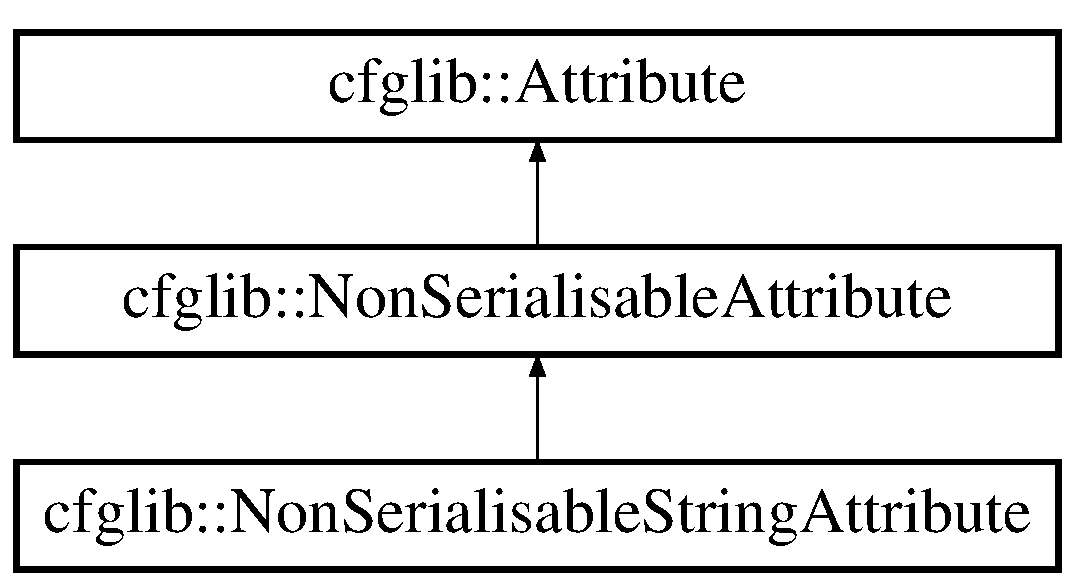
\includegraphics[height=3.000000cm]{classcfglib_1_1NonSerialisableStringAttribute}
\end{center}
\end{figure}
\subsection*{Public Member Functions}
\begin{DoxyCompactItemize}
\item 
\hyperlink{classcfglib_1_1NonSerialisableStringAttribute_a7f6f569a83349f8f41d187df56a43b65}{Non\+Serialisable\+String\+Attribute} (std\+::string const \&val)
\item 
\hyperlink{classcfglib_1_1NonSerialisableStringAttribute_a1432b55b0449e2fd8bdb8d6d7232b056}{Non\+Serialisable\+String\+Attribute} ()
\item 
virtual \hyperlink{classcfglib_1_1NonSerialisableStringAttribute}{Non\+Serialisable\+String\+Attribute} $\ast$ \hyperlink{classcfglib_1_1NonSerialisableStringAttribute_a5a7857efb5a59c478ef31266ddfd2f2c}{clone} ()
\item 
void \hyperlink{classcfglib_1_1NonSerialisableStringAttribute_aedeb7ccd57b84ed2e3bcfc464038682e}{Print} (std\+::ostream \&s)
\item 
std\+::string \hyperlink{classcfglib_1_1NonSerialisableStringAttribute_a3fb5338650a4569eb9b22b5419c9b6b5}{Get\+Value} ()
\item 
void \hyperlink{classcfglib_1_1NonSerialisableStringAttribute_a708afb5de2e1139c2119589c3e8bd434}{Set\+Value} (std\+::string val)
\end{DoxyCompactItemize}
\subsection*{Additional Inherited Members}


\subsection{Detailed Description}
\hyperlink{classcfglib_1_1NonSerialisableStringAttribute}{Non\+Serialisable\+String\+Attribute} is a library-\/supported non serialisable attribute of type string 

\subsection{Constructor \& Destructor Documentation}
\mbox{\Hypertarget{classcfglib_1_1NonSerialisableStringAttribute_a7f6f569a83349f8f41d187df56a43b65}\label{classcfglib_1_1NonSerialisableStringAttribute_a7f6f569a83349f8f41d187df56a43b65}} 
\index{cfglib\+::\+Non\+Serialisable\+String\+Attribute@{cfglib\+::\+Non\+Serialisable\+String\+Attribute}!Non\+Serialisable\+String\+Attribute@{Non\+Serialisable\+String\+Attribute}}
\index{Non\+Serialisable\+String\+Attribute@{Non\+Serialisable\+String\+Attribute}!cfglib\+::\+Non\+Serialisable\+String\+Attribute@{cfglib\+::\+Non\+Serialisable\+String\+Attribute}}
\subsubsection{\texorpdfstring{Non\+Serialisable\+String\+Attribute()}{NonSerialisableStringAttribute()}\hspace{0.1cm}{\footnotesize\ttfamily [1/2]}}
{\footnotesize\ttfamily cfglib\+::\+Non\+Serialisable\+String\+Attribute\+::\+Non\+Serialisable\+String\+Attribute (\begin{DoxyParamCaption}\item[{std\+::string const \&}]{val }\end{DoxyParamCaption})\hspace{0.3cm}{\ttfamily [inline]}}

Constructor \mbox{\Hypertarget{classcfglib_1_1NonSerialisableStringAttribute_a1432b55b0449e2fd8bdb8d6d7232b056}\label{classcfglib_1_1NonSerialisableStringAttribute_a1432b55b0449e2fd8bdb8d6d7232b056}} 
\index{cfglib\+::\+Non\+Serialisable\+String\+Attribute@{cfglib\+::\+Non\+Serialisable\+String\+Attribute}!Non\+Serialisable\+String\+Attribute@{Non\+Serialisable\+String\+Attribute}}
\index{Non\+Serialisable\+String\+Attribute@{Non\+Serialisable\+String\+Attribute}!cfglib\+::\+Non\+Serialisable\+String\+Attribute@{cfglib\+::\+Non\+Serialisable\+String\+Attribute}}
\subsubsection{\texorpdfstring{Non\+Serialisable\+String\+Attribute()}{NonSerialisableStringAttribute()}\hspace{0.1cm}{\footnotesize\ttfamily [2/2]}}
{\footnotesize\ttfamily cfglib\+::\+Non\+Serialisable\+String\+Attribute\+::\+Non\+Serialisable\+String\+Attribute (\begin{DoxyParamCaption}{ }\end{DoxyParamCaption})\hspace{0.3cm}{\ttfamily [inline]}}

default constructor. 

\subsection{Member Function Documentation}
\mbox{\Hypertarget{classcfglib_1_1NonSerialisableStringAttribute_a5a7857efb5a59c478ef31266ddfd2f2c}\label{classcfglib_1_1NonSerialisableStringAttribute_a5a7857efb5a59c478ef31266ddfd2f2c}} 
\index{cfglib\+::\+Non\+Serialisable\+String\+Attribute@{cfglib\+::\+Non\+Serialisable\+String\+Attribute}!clone@{clone}}
\index{clone@{clone}!cfglib\+::\+Non\+Serialisable\+String\+Attribute@{cfglib\+::\+Non\+Serialisable\+String\+Attribute}}
\subsubsection{\texorpdfstring{clone()}{clone()}}
{\footnotesize\ttfamily virtual \hyperlink{classcfglib_1_1NonSerialisableStringAttribute}{Non\+Serialisable\+String\+Attribute}$\ast$ cfglib\+::\+Non\+Serialisable\+String\+Attribute\+::clone (\begin{DoxyParamCaption}{ }\end{DoxyParamCaption})\hspace{0.3cm}{\ttfamily [inline]}, {\ttfamily [virtual]}}

virtual constructor 

Implements \hyperlink{classcfglib_1_1Attribute_a107366042fdafe881215426059fec3f8}{cfglib\+::\+Attribute}.

\mbox{\Hypertarget{classcfglib_1_1NonSerialisableStringAttribute_a3fb5338650a4569eb9b22b5419c9b6b5}\label{classcfglib_1_1NonSerialisableStringAttribute_a3fb5338650a4569eb9b22b5419c9b6b5}} 
\index{cfglib\+::\+Non\+Serialisable\+String\+Attribute@{cfglib\+::\+Non\+Serialisable\+String\+Attribute}!Get\+Value@{Get\+Value}}
\index{Get\+Value@{Get\+Value}!cfglib\+::\+Non\+Serialisable\+String\+Attribute@{cfglib\+::\+Non\+Serialisable\+String\+Attribute}}
\subsubsection{\texorpdfstring{Get\+Value()}{GetValue()}}
{\footnotesize\ttfamily std\+::string cfglib\+::\+Non\+Serialisable\+String\+Attribute\+::\+Get\+Value (\begin{DoxyParamCaption}{ }\end{DoxyParamCaption})\hspace{0.3cm}{\ttfamily [inline]}}

get std\+::string value of the String \hyperlink{classcfglib_1_1Attribute}{Attribute} \mbox{\Hypertarget{classcfglib_1_1NonSerialisableStringAttribute_aedeb7ccd57b84ed2e3bcfc464038682e}\label{classcfglib_1_1NonSerialisableStringAttribute_aedeb7ccd57b84ed2e3bcfc464038682e}} 
\index{cfglib\+::\+Non\+Serialisable\+String\+Attribute@{cfglib\+::\+Non\+Serialisable\+String\+Attribute}!Print@{Print}}
\index{Print@{Print}!cfglib\+::\+Non\+Serialisable\+String\+Attribute@{cfglib\+::\+Non\+Serialisable\+String\+Attribute}}
\subsubsection{\texorpdfstring{Print()}{Print()}}
{\footnotesize\ttfamily void cfglib\+::\+Non\+Serialisable\+String\+Attribute\+::\+Print (\begin{DoxyParamCaption}\item[{std\+::ostream \&}]{s }\end{DoxyParamCaption})\hspace{0.3cm}{\ttfamily [inline]}, {\ttfamily [virtual]}}

\hyperlink{classcfglib_1_1Attribute}{Attribute} printing function (debug only) 

Implements \hyperlink{classcfglib_1_1Attribute_af8d87ceddde146b92727e61823e0129b}{cfglib\+::\+Attribute}.

\mbox{\Hypertarget{classcfglib_1_1NonSerialisableStringAttribute_a708afb5de2e1139c2119589c3e8bd434}\label{classcfglib_1_1NonSerialisableStringAttribute_a708afb5de2e1139c2119589c3e8bd434}} 
\index{cfglib\+::\+Non\+Serialisable\+String\+Attribute@{cfglib\+::\+Non\+Serialisable\+String\+Attribute}!Set\+Value@{Set\+Value}}
\index{Set\+Value@{Set\+Value}!cfglib\+::\+Non\+Serialisable\+String\+Attribute@{cfglib\+::\+Non\+Serialisable\+String\+Attribute}}
\subsubsection{\texorpdfstring{Set\+Value()}{SetValue()}}
{\footnotesize\ttfamily void cfglib\+::\+Non\+Serialisable\+String\+Attribute\+::\+Set\+Value (\begin{DoxyParamCaption}\item[{std\+::string}]{val }\end{DoxyParamCaption})\hspace{0.3cm}{\ttfamily [inline]}}

set the value of the String attribute 

The documentation for this class was generated from the following file\+:\begin{DoxyCompactItemize}
\item 
include/\hyperlink{NonSerialisableAttributes_8h}{Non\+Serialisable\+Attributes.\+h}\end{DoxyCompactItemize}

\hypertarget{classcfglib_1_1NonSerialisableUnsignedLongAttribute}{}\section{cfglib\+:\+:Non\+Serialisable\+Unsigned\+Long\+Attribute Class Reference}
\label{classcfglib_1_1NonSerialisableUnsignedLongAttribute}\index{cfglib\+::\+Non\+Serialisable\+Unsigned\+Long\+Attribute@{cfglib\+::\+Non\+Serialisable\+Unsigned\+Long\+Attribute}}


{\ttfamily \#include $<$Non\+Serialisable\+Attributes.\+h$>$}

Inheritance diagram for cfglib\+:\+:Non\+Serialisable\+Unsigned\+Long\+Attribute\+:\begin{figure}[H]
\begin{center}
\leavevmode
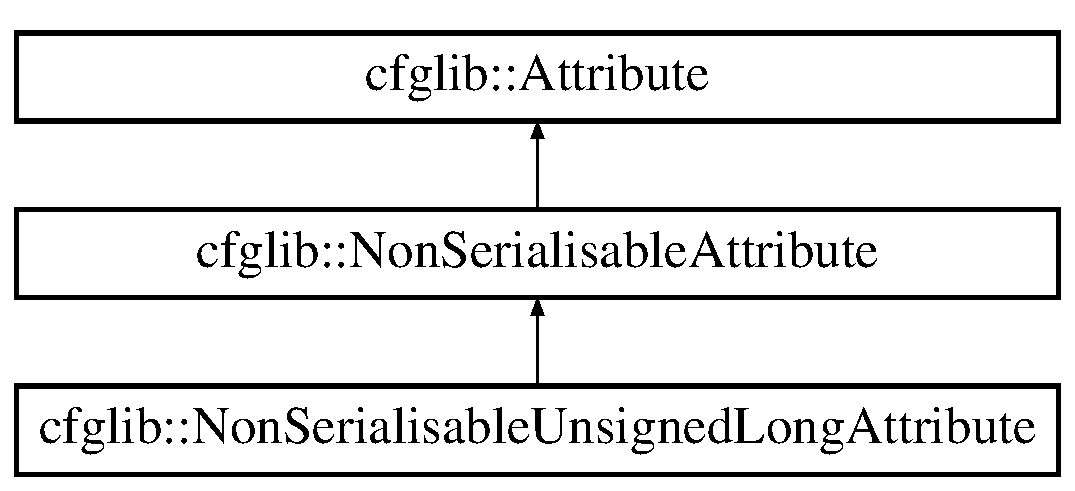
\includegraphics[height=3.000000cm]{classcfglib_1_1NonSerialisableUnsignedLongAttribute}
\end{center}
\end{figure}
\subsection*{Public Member Functions}
\begin{DoxyCompactItemize}
\item 
\hyperlink{classcfglib_1_1NonSerialisableUnsignedLongAttribute_a898beaee191d410f062ff7b839a51039}{Non\+Serialisable\+Unsigned\+Long\+Attribute} (unsigned long val)
\item 
\hyperlink{classcfglib_1_1NonSerialisableUnsignedLongAttribute_ae083d3614a66047ab325a009a7db88a5}{Non\+Serialisable\+Unsigned\+Long\+Attribute} ()
\item 
virtual \hyperlink{classcfglib_1_1NonSerialisableUnsignedLongAttribute}{Non\+Serialisable\+Unsigned\+Long\+Attribute} $\ast$ \hyperlink{classcfglib_1_1NonSerialisableUnsignedLongAttribute_a3c01da3fbc7e617c7a919716a1142f57}{clone} ()
\item 
void \hyperlink{classcfglib_1_1NonSerialisableUnsignedLongAttribute_aef0e4a5bc60b6d4f278ab2daa553f598}{Print} (std\+::ostream \&s)
\item 
unsigned long \hyperlink{classcfglib_1_1NonSerialisableUnsignedLongAttribute_aedeced928ce8d3de8b0a691371b6aded}{Get\+Value} ()
\item 
void \hyperlink{classcfglib_1_1NonSerialisableUnsignedLongAttribute_aea6d8fd0b4f145dc69d54f21d95f09cc}{Set\+Value} (unsigned long v)
\end{DoxyCompactItemize}
\subsection*{Additional Inherited Members}


\subsection{Detailed Description}
\hyperlink{classcfglib_1_1NonSerialisableUnsignedLongAttribute}{Non\+Serialisable\+Unsigned\+Long\+Attribute} is a library-\/supported non serialisable attribute of type unsigned long 

\subsection{Constructor \& Destructor Documentation}
\mbox{\Hypertarget{classcfglib_1_1NonSerialisableUnsignedLongAttribute_a898beaee191d410f062ff7b839a51039}\label{classcfglib_1_1NonSerialisableUnsignedLongAttribute_a898beaee191d410f062ff7b839a51039}} 
\index{cfglib\+::\+Non\+Serialisable\+Unsigned\+Long\+Attribute@{cfglib\+::\+Non\+Serialisable\+Unsigned\+Long\+Attribute}!Non\+Serialisable\+Unsigned\+Long\+Attribute@{Non\+Serialisable\+Unsigned\+Long\+Attribute}}
\index{Non\+Serialisable\+Unsigned\+Long\+Attribute@{Non\+Serialisable\+Unsigned\+Long\+Attribute}!cfglib\+::\+Non\+Serialisable\+Unsigned\+Long\+Attribute@{cfglib\+::\+Non\+Serialisable\+Unsigned\+Long\+Attribute}}
\subsubsection{\texorpdfstring{Non\+Serialisable\+Unsigned\+Long\+Attribute()}{NonSerialisableUnsignedLongAttribute()}\hspace{0.1cm}{\footnotesize\ttfamily [1/2]}}
{\footnotesize\ttfamily cfglib\+::\+Non\+Serialisable\+Unsigned\+Long\+Attribute\+::\+Non\+Serialisable\+Unsigned\+Long\+Attribute (\begin{DoxyParamCaption}\item[{unsigned long}]{val }\end{DoxyParamCaption})\hspace{0.3cm}{\ttfamily [inline]}}

Constructor \mbox{\Hypertarget{classcfglib_1_1NonSerialisableUnsignedLongAttribute_ae083d3614a66047ab325a009a7db88a5}\label{classcfglib_1_1NonSerialisableUnsignedLongAttribute_ae083d3614a66047ab325a009a7db88a5}} 
\index{cfglib\+::\+Non\+Serialisable\+Unsigned\+Long\+Attribute@{cfglib\+::\+Non\+Serialisable\+Unsigned\+Long\+Attribute}!Non\+Serialisable\+Unsigned\+Long\+Attribute@{Non\+Serialisable\+Unsigned\+Long\+Attribute}}
\index{Non\+Serialisable\+Unsigned\+Long\+Attribute@{Non\+Serialisable\+Unsigned\+Long\+Attribute}!cfglib\+::\+Non\+Serialisable\+Unsigned\+Long\+Attribute@{cfglib\+::\+Non\+Serialisable\+Unsigned\+Long\+Attribute}}
\subsubsection{\texorpdfstring{Non\+Serialisable\+Unsigned\+Long\+Attribute()}{NonSerialisableUnsignedLongAttribute()}\hspace{0.1cm}{\footnotesize\ttfamily [2/2]}}
{\footnotesize\ttfamily cfglib\+::\+Non\+Serialisable\+Unsigned\+Long\+Attribute\+::\+Non\+Serialisable\+Unsigned\+Long\+Attribute (\begin{DoxyParamCaption}{ }\end{DoxyParamCaption})\hspace{0.3cm}{\ttfamily [inline]}}

default constructor. 

\subsection{Member Function Documentation}
\mbox{\Hypertarget{classcfglib_1_1NonSerialisableUnsignedLongAttribute_a3c01da3fbc7e617c7a919716a1142f57}\label{classcfglib_1_1NonSerialisableUnsignedLongAttribute_a3c01da3fbc7e617c7a919716a1142f57}} 
\index{cfglib\+::\+Non\+Serialisable\+Unsigned\+Long\+Attribute@{cfglib\+::\+Non\+Serialisable\+Unsigned\+Long\+Attribute}!clone@{clone}}
\index{clone@{clone}!cfglib\+::\+Non\+Serialisable\+Unsigned\+Long\+Attribute@{cfglib\+::\+Non\+Serialisable\+Unsigned\+Long\+Attribute}}
\subsubsection{\texorpdfstring{clone()}{clone()}}
{\footnotesize\ttfamily virtual \hyperlink{classcfglib_1_1NonSerialisableUnsignedLongAttribute}{Non\+Serialisable\+Unsigned\+Long\+Attribute}$\ast$ cfglib\+::\+Non\+Serialisable\+Unsigned\+Long\+Attribute\+::clone (\begin{DoxyParamCaption}{ }\end{DoxyParamCaption})\hspace{0.3cm}{\ttfamily [inline]}, {\ttfamily [virtual]}}

virtual constructor 

Implements \hyperlink{classcfglib_1_1Attribute_a107366042fdafe881215426059fec3f8}{cfglib\+::\+Attribute}.

\mbox{\Hypertarget{classcfglib_1_1NonSerialisableUnsignedLongAttribute_aedeced928ce8d3de8b0a691371b6aded}\label{classcfglib_1_1NonSerialisableUnsignedLongAttribute_aedeced928ce8d3de8b0a691371b6aded}} 
\index{cfglib\+::\+Non\+Serialisable\+Unsigned\+Long\+Attribute@{cfglib\+::\+Non\+Serialisable\+Unsigned\+Long\+Attribute}!Get\+Value@{Get\+Value}}
\index{Get\+Value@{Get\+Value}!cfglib\+::\+Non\+Serialisable\+Unsigned\+Long\+Attribute@{cfglib\+::\+Non\+Serialisable\+Unsigned\+Long\+Attribute}}
\subsubsection{\texorpdfstring{Get\+Value()}{GetValue()}}
{\footnotesize\ttfamily unsigned long cfglib\+::\+Non\+Serialisable\+Unsigned\+Long\+Attribute\+::\+Get\+Value (\begin{DoxyParamCaption}{ }\end{DoxyParamCaption})\hspace{0.3cm}{\ttfamily [inline]}}

get int value of the Unsigned\+Long \hyperlink{classcfglib_1_1Attribute}{Attribute} \mbox{\Hypertarget{classcfglib_1_1NonSerialisableUnsignedLongAttribute_aef0e4a5bc60b6d4f278ab2daa553f598}\label{classcfglib_1_1NonSerialisableUnsignedLongAttribute_aef0e4a5bc60b6d4f278ab2daa553f598}} 
\index{cfglib\+::\+Non\+Serialisable\+Unsigned\+Long\+Attribute@{cfglib\+::\+Non\+Serialisable\+Unsigned\+Long\+Attribute}!Print@{Print}}
\index{Print@{Print}!cfglib\+::\+Non\+Serialisable\+Unsigned\+Long\+Attribute@{cfglib\+::\+Non\+Serialisable\+Unsigned\+Long\+Attribute}}
\subsubsection{\texorpdfstring{Print()}{Print()}}
{\footnotesize\ttfamily void cfglib\+::\+Non\+Serialisable\+Unsigned\+Long\+Attribute\+::\+Print (\begin{DoxyParamCaption}\item[{std\+::ostream \&}]{s }\end{DoxyParamCaption})\hspace{0.3cm}{\ttfamily [inline]}, {\ttfamily [virtual]}}

\hyperlink{classcfglib_1_1Attribute}{Attribute} printing function (debug only) 

Implements \hyperlink{classcfglib_1_1Attribute_af8d87ceddde146b92727e61823e0129b}{cfglib\+::\+Attribute}.

\mbox{\Hypertarget{classcfglib_1_1NonSerialisableUnsignedLongAttribute_aea6d8fd0b4f145dc69d54f21d95f09cc}\label{classcfglib_1_1NonSerialisableUnsignedLongAttribute_aea6d8fd0b4f145dc69d54f21d95f09cc}} 
\index{cfglib\+::\+Non\+Serialisable\+Unsigned\+Long\+Attribute@{cfglib\+::\+Non\+Serialisable\+Unsigned\+Long\+Attribute}!Set\+Value@{Set\+Value}}
\index{Set\+Value@{Set\+Value}!cfglib\+::\+Non\+Serialisable\+Unsigned\+Long\+Attribute@{cfglib\+::\+Non\+Serialisable\+Unsigned\+Long\+Attribute}}
\subsubsection{\texorpdfstring{Set\+Value()}{SetValue()}}
{\footnotesize\ttfamily void cfglib\+::\+Non\+Serialisable\+Unsigned\+Long\+Attribute\+::\+Set\+Value (\begin{DoxyParamCaption}\item[{unsigned long}]{v }\end{DoxyParamCaption})\hspace{0.3cm}{\ttfamily [inline]}}

set the value of the Unsigned\+Long \hyperlink{classcfglib_1_1Attribute}{Attribute} 

The documentation for this class was generated from the following file\+:\begin{DoxyCompactItemize}
\item 
include/\hyperlink{NonSerialisableAttributes_8h}{Non\+Serialisable\+Attributes.\+h}\end{DoxyCompactItemize}

\hypertarget{classcfglib_1_1Program}{}\section{cfglib\+:\+:Program Class Reference}
\label{classcfglib_1_1Program}\index{cfglib\+::\+Program@{cfglib\+::\+Program}}


{\ttfamily \#include $<$Program.\+h$>$}

Inheritance diagram for cfglib\+:\+:Program\+:\begin{figure}[H]
\begin{center}
\leavevmode
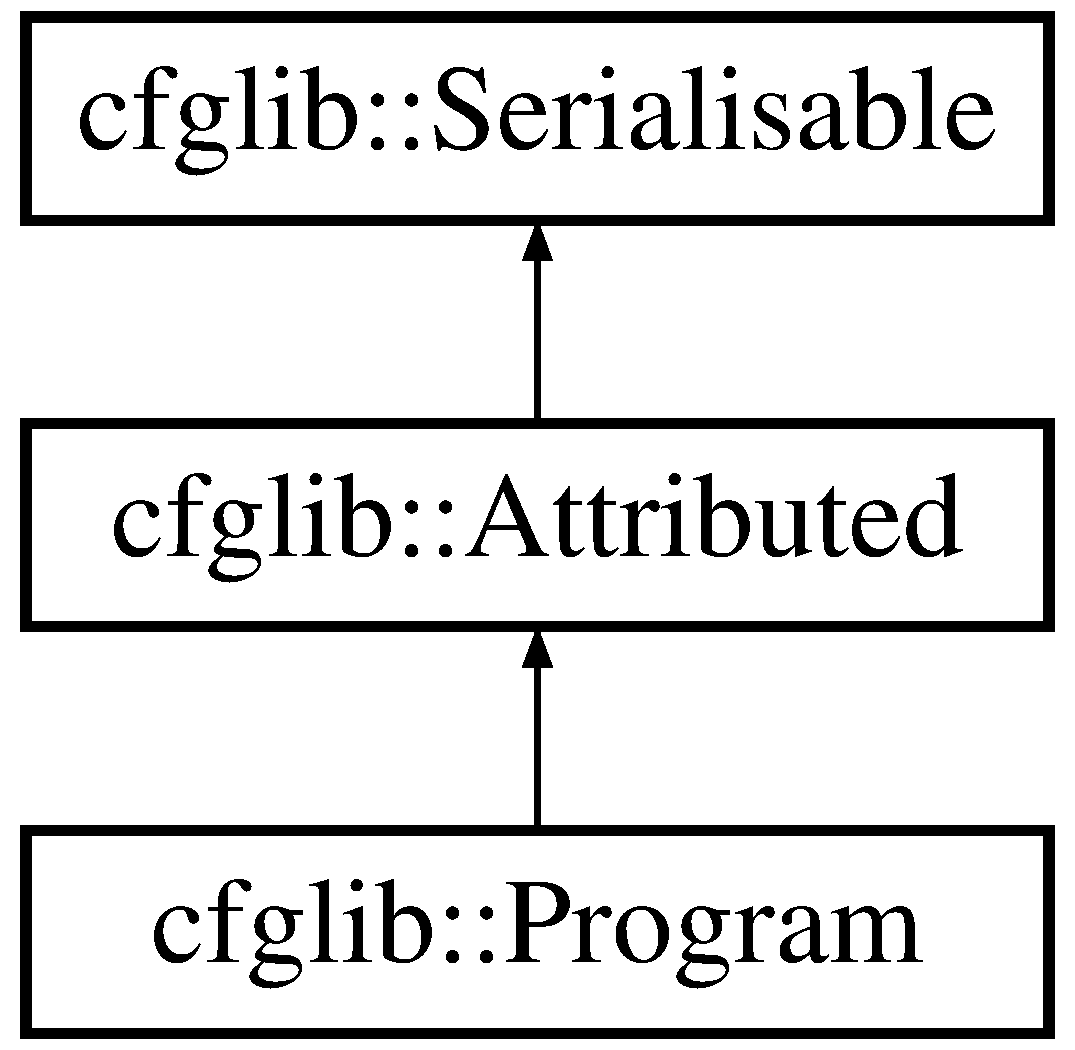
\includegraphics[height=3.000000cm]{classcfglib_1_1Program}
\end{center}
\end{figure}
\subsection*{Public Member Functions}
\begin{DoxyCompactItemize}
\item 
\hyperlink{classcfglib_1_1Program_ad18f1e51efad67f4d553e1de3d5aea55}{Program} (string pgm\+\_\+name)
\item 
\hyperlink{classcfglib_1_1Program_a96682ca2803d6f070767e8449c64eeac}{Program} ()
\item 
\hyperlink{classcfglib_1_1Program}{Program} $\ast$ \hyperlink{classcfglib_1_1Program_a6060c2b04628609085a7e50fdce5dec3}{Clone} ()
\item 
\hyperlink{classcfglib_1_1Program_a91470a76911e981b750085ce19668c34}{$\sim$\+Program} ()
\item 
string \hyperlink{classcfglib_1_1Program_acc4f72ffe5f628e35b0f063d4c3f9e9d}{Get\+Name} () const
\item 
void \hyperlink{classcfglib_1_1Program_acfcd600e324f86042ce08d27ec506cc2}{Set\+Name} (string pgm\+\_\+name)
\item 
\hyperlink{classcfglib_1_1Cfg}{Cfg} $\ast$ \hyperlink{classcfglib_1_1Program_ac8050c9c5e4905f5e27b3071abefba82}{Create\+New\+Cfg} (List\+Of\+String const \&lnames)
\item 
bool \hyperlink{classcfglib_1_1Program_a08aa67ec59bdbd28572dc222fdd2e3da}{Set\+Entry\+Point} (string entry\+\_\+point\+\_\+name)
\item 
void \hyperlink{classcfglib_1_1Program_a9afd774f6cdaed6441b3ecd37887ecd3}{Set\+Entry\+Point} (\hyperlink{classcfglib_1_1Cfg}{Cfg} $\ast$function)
\item 
\hyperlink{classcfglib_1_1Cfg}{Cfg} $\ast$ \hyperlink{classcfglib_1_1Program_a9223048335b62778f7823825a842d0da}{Get\+Entry\+Point} ()
\item 
\hyperlink{namespacecfglib_a6d40ca49d73d6bd01cf38af88645373a}{list\+Of\+Cfg} \hyperlink{classcfglib_1_1Program_a12869527820e336393106010b15ac419}{Get\+All\+Cfgs} ()
\item 
int \hyperlink{classcfglib_1_1Program_abd621c3512b0affedf904d6acbe9941b}{Get\+Nb\+Cfgs} ()
\item 
\hyperlink{classcfglib_1_1Cfg}{Cfg} $\ast$ \hyperlink{classcfglib_1_1Program_a78a1fa44a467ae9e897aea3710f7e931}{Get\+Cfg\+By\+Name} (std\+::string name)
\item 
\hyperlink{classcfglib_1_1Cfg}{Cfg} $\ast$ \hyperlink{classcfglib_1_1Program_a35902ab795a8defb794e0db1ececdf54}{Get\+Cfg\+By\+Num} (int index)
\item 
virtual std\+::ostream \& \hyperlink{classcfglib_1_1Program_af18db304f16fea3e395fbeb7d6a7b358}{Write\+Xml} (std\+::ostream \&os, \hyperlink{classcfglib_1_1Handle}{Handle} \&\hyperlink{classcfglib_1_1Program_a13cc0a03cdf31ab9cfa9a0a7b0dff8ed}{hand})
\item 
virtual void \hyperlink{classcfglib_1_1Program_ad854304f1126c700757fb461a36c8cbd}{Read\+Xml} (\hyperlink{classXmlTag}{Xml\+Tag} const $\ast$tag, \hyperlink{classcfglib_1_1Handle}{Handle} \&\hyperlink{classcfglib_1_1Program_a13cc0a03cdf31ab9cfa9a0a7b0dff8ed}{hand})
\item 
std\+::ostream \& \hyperlink{classcfglib_1_1Program_a50b65e054b0e6c2a6517e1f7c8a34379}{serialise\+\_\+program} (std\+::ostream \&os)
\item 
void \hyperlink{classcfglib_1_1Program_a2eb2e99e2d6dfbb346e23bebba01d2b3}{serialise\+\_\+program} (std\+::string \&file\+\_\+name)
\end{DoxyCompactItemize}
\subsection*{Static Public Member Functions}
\begin{DoxyCompactItemize}
\item 
static \hyperlink{classcfglib_1_1Program}{Program} $\ast$ \hyperlink{classcfglib_1_1Program_af486d3bd0aac88830c13289e5a416f07}{unserialise\+\_\+program\+\_\+file} (std\+::string const \&file\+\_\+name)
\end{DoxyCompactItemize}
\subsection*{Public Attributes}
\begin{DoxyCompactItemize}
\item 
\hyperlink{classcfglib_1_1Handle}{Handle} \hyperlink{classcfglib_1_1Program_a13cc0a03cdf31ab9cfa9a0a7b0dff8ed}{hand}
\end{DoxyCompactItemize}


\subsection{Detailed Description}
This class represents a program. A program is a set of functions each with a corresponding C\+FG. A program has one entry point. 

\subsection{Constructor \& Destructor Documentation}
\mbox{\Hypertarget{classcfglib_1_1Program_ad18f1e51efad67f4d553e1de3d5aea55}\label{classcfglib_1_1Program_ad18f1e51efad67f4d553e1de3d5aea55}} 
\index{cfglib\+::\+Program@{cfglib\+::\+Program}!Program@{Program}}
\index{Program@{Program}!cfglib\+::\+Program@{cfglib\+::\+Program}}
\subsubsection{\texorpdfstring{Program()}{Program()}\hspace{0.1cm}{\footnotesize\ttfamily [1/2]}}
{\footnotesize\ttfamily cfglib\+::\+Program\+::\+Program (\begin{DoxyParamCaption}\item[{string}]{pgm\+\_\+name }\end{DoxyParamCaption})}

constructor \mbox{\Hypertarget{classcfglib_1_1Program_a96682ca2803d6f070767e8449c64eeac}\label{classcfglib_1_1Program_a96682ca2803d6f070767e8449c64eeac}} 
\index{cfglib\+::\+Program@{cfglib\+::\+Program}!Program@{Program}}
\index{Program@{Program}!cfglib\+::\+Program@{cfglib\+::\+Program}}
\subsubsection{\texorpdfstring{Program()}{Program()}\hspace{0.1cm}{\footnotesize\ttfamily [2/2]}}
{\footnotesize\ttfamily cfglib\+::\+Program\+::\+Program (\begin{DoxyParamCaption}{ }\end{DoxyParamCaption})}

\mbox{\Hypertarget{classcfglib_1_1Program_a91470a76911e981b750085ce19668c34}\label{classcfglib_1_1Program_a91470a76911e981b750085ce19668c34}} 
\index{cfglib\+::\+Program@{cfglib\+::\+Program}!````~Program@{$\sim$\+Program}}
\index{````~Program@{$\sim$\+Program}!cfglib\+::\+Program@{cfglib\+::\+Program}}
\subsubsection{\texorpdfstring{$\sim$\+Program()}{~Program()}}
{\footnotesize\ttfamily cfglib\+::\+Program\+::$\sim$\+Program (\begin{DoxyParamCaption}{ }\end{DoxyParamCaption})}

destructor 

\subsection{Member Function Documentation}
\mbox{\Hypertarget{classcfglib_1_1Program_a6060c2b04628609085a7e50fdce5dec3}\label{classcfglib_1_1Program_a6060c2b04628609085a7e50fdce5dec3}} 
\index{cfglib\+::\+Program@{cfglib\+::\+Program}!Clone@{Clone}}
\index{Clone@{Clone}!cfglib\+::\+Program@{cfglib\+::\+Program}}
\subsubsection{\texorpdfstring{Clone()}{Clone()}}
{\footnotesize\ttfamily \hyperlink{classcfglib_1_1Program}{Program}$\ast$ cfglib\+::\+Program\+::\+Clone (\begin{DoxyParamCaption}{ }\end{DoxyParamCaption})}

clone the program \mbox{\Hypertarget{classcfglib_1_1Program_ac8050c9c5e4905f5e27b3071abefba82}\label{classcfglib_1_1Program_ac8050c9c5e4905f5e27b3071abefba82}} 
\index{cfglib\+::\+Program@{cfglib\+::\+Program}!Create\+New\+Cfg@{Create\+New\+Cfg}}
\index{Create\+New\+Cfg@{Create\+New\+Cfg}!cfglib\+::\+Program@{cfglib\+::\+Program}}
\subsubsection{\texorpdfstring{Create\+New\+Cfg()}{CreateNewCfg()}}
{\footnotesize\ttfamily \hyperlink{classcfglib_1_1Cfg}{Cfg}$\ast$ cfglib\+::\+Program\+::\+Create\+New\+Cfg (\begin{DoxyParamCaption}\item[{List\+Of\+String const \&}]{lnames }\end{DoxyParamCaption})}

Add \hyperlink{classcfglib_1_1Cfg}{Cfg} (functions) to \hyperlink{classcfglib_1_1Program}{Program}. The value returned is valid only as long as this \hyperlink{classcfglib_1_1Program}{Program} exists. It must not be used in two diferent Programs. The first created \hyperlink{classcfglib_1_1Cfg}{Cfg} is the entry point. \mbox{\Hypertarget{classcfglib_1_1Program_a12869527820e336393106010b15ac419}\label{classcfglib_1_1Program_a12869527820e336393106010b15ac419}} 
\index{cfglib\+::\+Program@{cfglib\+::\+Program}!Get\+All\+Cfgs@{Get\+All\+Cfgs}}
\index{Get\+All\+Cfgs@{Get\+All\+Cfgs}!cfglib\+::\+Program@{cfglib\+::\+Program}}
\subsubsection{\texorpdfstring{Get\+All\+Cfgs()}{GetAllCfgs()}}
{\footnotesize\ttfamily \hyperlink{namespacecfglib_a6d40ca49d73d6bd01cf38af88645373a}{list\+Of\+Cfg} cfglib\+::\+Program\+::\+Get\+All\+Cfgs (\begin{DoxyParamCaption}{ }\end{DoxyParamCaption})}

get the list of Cfgs of the program. \mbox{\Hypertarget{classcfglib_1_1Program_a78a1fa44a467ae9e897aea3710f7e931}\label{classcfglib_1_1Program_a78a1fa44a467ae9e897aea3710f7e931}} 
\index{cfglib\+::\+Program@{cfglib\+::\+Program}!Get\+Cfg\+By\+Name@{Get\+Cfg\+By\+Name}}
\index{Get\+Cfg\+By\+Name@{Get\+Cfg\+By\+Name}!cfglib\+::\+Program@{cfglib\+::\+Program}}
\subsubsection{\texorpdfstring{Get\+Cfg\+By\+Name()}{GetCfgByName()}}
{\footnotesize\ttfamily \hyperlink{classcfglib_1_1Cfg}{Cfg}$\ast$ cfglib\+::\+Program\+::\+Get\+Cfg\+By\+Name (\begin{DoxyParamCaption}\item[{std\+::string}]{name }\end{DoxyParamCaption})}

return the \hyperlink{classcfglib_1_1Cfg}{Cfg} with a specified name, 0 if it does not exists \mbox{\Hypertarget{classcfglib_1_1Program_a35902ab795a8defb794e0db1ececdf54}\label{classcfglib_1_1Program_a35902ab795a8defb794e0db1ececdf54}} 
\index{cfglib\+::\+Program@{cfglib\+::\+Program}!Get\+Cfg\+By\+Num@{Get\+Cfg\+By\+Num}}
\index{Get\+Cfg\+By\+Num@{Get\+Cfg\+By\+Num}!cfglib\+::\+Program@{cfglib\+::\+Program}}
\subsubsection{\texorpdfstring{Get\+Cfg\+By\+Num()}{GetCfgByNum()}}
{\footnotesize\ttfamily \hyperlink{classcfglib_1_1Cfg}{Cfg}$\ast$ cfglib\+::\+Program\+::\+Get\+Cfg\+By\+Num (\begin{DoxyParamCaption}\item[{int}]{index }\end{DoxyParamCaption})}

Return the \hyperlink{classcfglib_1_1Cfg}{Cfg} with a specific number in the list of Cfgs (starting by index 0) or 0 if the index does not exist \mbox{\Hypertarget{classcfglib_1_1Program_a9223048335b62778f7823825a842d0da}\label{classcfglib_1_1Program_a9223048335b62778f7823825a842d0da}} 
\index{cfglib\+::\+Program@{cfglib\+::\+Program}!Get\+Entry\+Point@{Get\+Entry\+Point}}
\index{Get\+Entry\+Point@{Get\+Entry\+Point}!cfglib\+::\+Program@{cfglib\+::\+Program}}
\subsubsection{\texorpdfstring{Get\+Entry\+Point()}{GetEntryPoint()}}
{\footnotesize\ttfamily \hyperlink{classcfglib_1_1Cfg}{Cfg}$\ast$ cfglib\+::\+Program\+::\+Get\+Entry\+Point (\begin{DoxyParamCaption}{ }\end{DoxyParamCaption})}

Get entry point of the program \mbox{\Hypertarget{classcfglib_1_1Program_acc4f72ffe5f628e35b0f063d4c3f9e9d}\label{classcfglib_1_1Program_acc4f72ffe5f628e35b0f063d4c3f9e9d}} 
\index{cfglib\+::\+Program@{cfglib\+::\+Program}!Get\+Name@{Get\+Name}}
\index{Get\+Name@{Get\+Name}!cfglib\+::\+Program@{cfglib\+::\+Program}}
\subsubsection{\texorpdfstring{Get\+Name()}{GetName()}}
{\footnotesize\ttfamily string cfglib\+::\+Program\+::\+Get\+Name (\begin{DoxyParamCaption}{ }\end{DoxyParamCaption}) const}

Get program name \mbox{\Hypertarget{classcfglib_1_1Program_abd621c3512b0affedf904d6acbe9941b}\label{classcfglib_1_1Program_abd621c3512b0affedf904d6acbe9941b}} 
\index{cfglib\+::\+Program@{cfglib\+::\+Program}!Get\+Nb\+Cfgs@{Get\+Nb\+Cfgs}}
\index{Get\+Nb\+Cfgs@{Get\+Nb\+Cfgs}!cfglib\+::\+Program@{cfglib\+::\+Program}}
\subsubsection{\texorpdfstring{Get\+Nb\+Cfgs()}{GetNbCfgs()}}
{\footnotesize\ttfamily int cfglib\+::\+Program\+::\+Get\+Nb\+Cfgs (\begin{DoxyParamCaption}{ }\end{DoxyParamCaption})\hspace{0.3cm}{\ttfamily [inline]}}

\mbox{\Hypertarget{classcfglib_1_1Program_ad854304f1126c700757fb461a36c8cbd}\label{classcfglib_1_1Program_ad854304f1126c700757fb461a36c8cbd}} 
\index{cfglib\+::\+Program@{cfglib\+::\+Program}!Read\+Xml@{Read\+Xml}}
\index{Read\+Xml@{Read\+Xml}!cfglib\+::\+Program@{cfglib\+::\+Program}}
\subsubsection{\texorpdfstring{Read\+Xml()}{ReadXml()}}
{\footnotesize\ttfamily virtual void cfglib\+::\+Program\+::\+Read\+Xml (\begin{DoxyParamCaption}\item[{\hyperlink{classXmlTag}{Xml\+Tag} const $\ast$}]{tag,  }\item[{\hyperlink{classcfglib_1_1Handle}{Handle} \&}]{hand }\end{DoxyParamCaption})\hspace{0.3cm}{\ttfamily [virtual]}}

Internal seserialisation function. 

Implements \hyperlink{classcfglib_1_1Serialisable_a876d530446317872259356af9b016e13}{cfglib\+::\+Serialisable}.

\mbox{\Hypertarget{classcfglib_1_1Program_a50b65e054b0e6c2a6517e1f7c8a34379}\label{classcfglib_1_1Program_a50b65e054b0e6c2a6517e1f7c8a34379}} 
\index{cfglib\+::\+Program@{cfglib\+::\+Program}!serialise\+\_\+program@{serialise\+\_\+program}}
\index{serialise\+\_\+program@{serialise\+\_\+program}!cfglib\+::\+Program@{cfglib\+::\+Program}}
\subsubsection{\texorpdfstring{serialise\+\_\+program()}{serialise\_program()}\hspace{0.1cm}{\footnotesize\ttfamily [1/2]}}
{\footnotesize\ttfamily std\+::ostream\& cfglib\+::\+Program\+::serialise\+\_\+program (\begin{DoxyParamCaption}\item[{std\+::ostream \&}]{os }\end{DoxyParamCaption})}

Serialisation function. \mbox{\Hypertarget{classcfglib_1_1Program_a2eb2e99e2d6dfbb346e23bebba01d2b3}\label{classcfglib_1_1Program_a2eb2e99e2d6dfbb346e23bebba01d2b3}} 
\index{cfglib\+::\+Program@{cfglib\+::\+Program}!serialise\+\_\+program@{serialise\+\_\+program}}
\index{serialise\+\_\+program@{serialise\+\_\+program}!cfglib\+::\+Program@{cfglib\+::\+Program}}
\subsubsection{\texorpdfstring{serialise\+\_\+program()}{serialise\_program()}\hspace{0.1cm}{\footnotesize\ttfamily [2/2]}}
{\footnotesize\ttfamily void cfglib\+::\+Program\+::serialise\+\_\+program (\begin{DoxyParamCaption}\item[{std\+::string \&}]{file\+\_\+name }\end{DoxyParamCaption})}

Serialisation to file function \mbox{\Hypertarget{classcfglib_1_1Program_a08aa67ec59bdbd28572dc222fdd2e3da}\label{classcfglib_1_1Program_a08aa67ec59bdbd28572dc222fdd2e3da}} 
\index{cfglib\+::\+Program@{cfglib\+::\+Program}!Set\+Entry\+Point@{Set\+Entry\+Point}}
\index{Set\+Entry\+Point@{Set\+Entry\+Point}!cfglib\+::\+Program@{cfglib\+::\+Program}}
\subsubsection{\texorpdfstring{Set\+Entry\+Point()}{SetEntryPoint()}\hspace{0.1cm}{\footnotesize\ttfamily [1/2]}}
{\footnotesize\ttfamily bool cfglib\+::\+Program\+::\+Set\+Entry\+Point (\begin{DoxyParamCaption}\item[{string}]{entry\+\_\+point\+\_\+name }\end{DoxyParamCaption})}

The cgf with entry\+\_\+point\+\_\+name as name, becomes the entry point of the program. \begin{DoxyReturn}{Returns}
true if the entry point exsits, false otherwise. 
\end{DoxyReturn}
\mbox{\Hypertarget{classcfglib_1_1Program_a9afd774f6cdaed6441b3ecd37887ecd3}\label{classcfglib_1_1Program_a9afd774f6cdaed6441b3ecd37887ecd3}} 
\index{cfglib\+::\+Program@{cfglib\+::\+Program}!Set\+Entry\+Point@{Set\+Entry\+Point}}
\index{Set\+Entry\+Point@{Set\+Entry\+Point}!cfglib\+::\+Program@{cfglib\+::\+Program}}
\subsubsection{\texorpdfstring{Set\+Entry\+Point()}{SetEntryPoint()}\hspace{0.1cm}{\footnotesize\ttfamily [2/2]}}
{\footnotesize\ttfamily void cfglib\+::\+Program\+::\+Set\+Entry\+Point (\begin{DoxyParamCaption}\item[{\hyperlink{classcfglib_1_1Cfg}{Cfg} $\ast$}]{function }\end{DoxyParamCaption})}

Set the entry point of this program. The \hyperlink{classcfglib_1_1Cfg}{Cfg} passed in argument must be a \hyperlink{classcfglib_1_1Cfg}{Cfg} of this \hyperlink{classcfglib_1_1Program}{Program}. \mbox{\Hypertarget{classcfglib_1_1Program_acfcd600e324f86042ce08d27ec506cc2}\label{classcfglib_1_1Program_acfcd600e324f86042ce08d27ec506cc2}} 
\index{cfglib\+::\+Program@{cfglib\+::\+Program}!Set\+Name@{Set\+Name}}
\index{Set\+Name@{Set\+Name}!cfglib\+::\+Program@{cfglib\+::\+Program}}
\subsubsection{\texorpdfstring{Set\+Name()}{SetName()}}
{\footnotesize\ttfamily void cfglib\+::\+Program\+::\+Set\+Name (\begin{DoxyParamCaption}\item[{string}]{pgm\+\_\+name }\end{DoxyParamCaption})}

Set program name \mbox{\Hypertarget{classcfglib_1_1Program_af486d3bd0aac88830c13289e5a416f07}\label{classcfglib_1_1Program_af486d3bd0aac88830c13289e5a416f07}} 
\index{cfglib\+::\+Program@{cfglib\+::\+Program}!unserialise\+\_\+program\+\_\+file@{unserialise\+\_\+program\+\_\+file}}
\index{unserialise\+\_\+program\+\_\+file@{unserialise\+\_\+program\+\_\+file}!cfglib\+::\+Program@{cfglib\+::\+Program}}
\subsubsection{\texorpdfstring{unserialise\+\_\+program\+\_\+file()}{unserialise\_program\_file()}}
{\footnotesize\ttfamily static \hyperlink{classcfglib_1_1Program}{Program}$\ast$ cfglib\+::\+Program\+::unserialise\+\_\+program\+\_\+file (\begin{DoxyParamCaption}\item[{std\+::string const \&}]{file\+\_\+name }\end{DoxyParamCaption})\hspace{0.3cm}{\ttfamily [static]}}

Deserialisation function. This function is the one really meant for user usage. Read\+Xml should not be used. cf. unserialise\+\_\+program for precision on arguments. \mbox{\Hypertarget{classcfglib_1_1Program_af18db304f16fea3e395fbeb7d6a7b358}\label{classcfglib_1_1Program_af18db304f16fea3e395fbeb7d6a7b358}} 
\index{cfglib\+::\+Program@{cfglib\+::\+Program}!Write\+Xml@{Write\+Xml}}
\index{Write\+Xml@{Write\+Xml}!cfglib\+::\+Program@{cfglib\+::\+Program}}
\subsubsection{\texorpdfstring{Write\+Xml()}{WriteXml()}}
{\footnotesize\ttfamily virtual std\+::ostream\& cfglib\+::\+Program\+::\+Write\+Xml (\begin{DoxyParamCaption}\item[{std\+::ostream \&}]{os,  }\item[{\hyperlink{classcfglib_1_1Handle}{Handle} \&}]{hand }\end{DoxyParamCaption})\hspace{0.3cm}{\ttfamily [virtual]}}

Serialisation function. 

Implements \hyperlink{classcfglib_1_1Serialisable_aaeb80cc7397ad312e5ae34f39412ce42}{cfglib\+::\+Serialisable}.



\subsection{Member Data Documentation}
\mbox{\Hypertarget{classcfglib_1_1Program_a13cc0a03cdf31ab9cfa9a0a7b0dff8ed}\label{classcfglib_1_1Program_a13cc0a03cdf31ab9cfa9a0a7b0dff8ed}} 
\index{cfglib\+::\+Program@{cfglib\+::\+Program}!hand@{hand}}
\index{hand@{hand}!cfglib\+::\+Program@{cfglib\+::\+Program}}
\subsubsection{\texorpdfstring{hand}{hand}}
{\footnotesize\ttfamily \hyperlink{classcfglib_1_1Handle}{Handle} cfglib\+::\+Program\+::hand}



The documentation for this class was generated from the following file\+:\begin{DoxyCompactItemize}
\item 
include/\hyperlink{Program_8h}{Program.\+h}\end{DoxyCompactItemize}

\hypertarget{classcfglib_1_1Serialisable}{}\section{cfglib\+:\+:Serialisable Class Reference}
\label{classcfglib_1_1Serialisable}\index{cfglib\+::\+Serialisable@{cfglib\+::\+Serialisable}}


{\ttfamily \#include $<$Serialisable.\+h$>$}

Inheritance diagram for cfglib\+:\+:Serialisable\+:\begin{figure}[H]
\begin{center}
\leavevmode
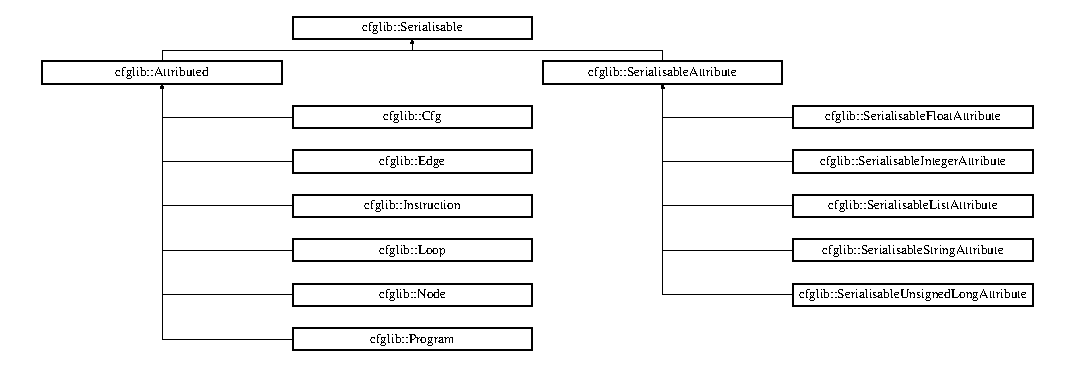
\includegraphics[height=4.480000cm]{classcfglib_1_1Serialisable}
\end{center}
\end{figure}
\subsection*{Public Member Functions}
\begin{DoxyCompactItemize}
\item 
virtual std\+::ostream \& \hyperlink{classcfglib_1_1Serialisable_aaeb80cc7397ad312e5ae34f39412ce42}{Write\+Xml} (std\+::ostream \&os, \hyperlink{classcfglib_1_1Handle}{Handle} \&hand)=0
\item 
virtual void \hyperlink{classcfglib_1_1Serialisable_a876d530446317872259356af9b016e13}{Read\+Xml} (\hyperlink{classXmlTag}{Xml\+Tag} const $\ast$tag, \hyperlink{classcfglib_1_1Handle}{Handle} \&hand)=0
\item 
virtual \hyperlink{classcfglib_1_1Serialisable_a778fac708aa3f3c1063fcadef60590ee}{$\sim$\+Serialisable} ()
\end{DoxyCompactItemize}


\subsection{Constructor \& Destructor Documentation}
\mbox{\Hypertarget{classcfglib_1_1Serialisable_a778fac708aa3f3c1063fcadef60590ee}\label{classcfglib_1_1Serialisable_a778fac708aa3f3c1063fcadef60590ee}} 
\index{cfglib\+::\+Serialisable@{cfglib\+::\+Serialisable}!````~Serialisable@{$\sim$\+Serialisable}}
\index{````~Serialisable@{$\sim$\+Serialisable}!cfglib\+::\+Serialisable@{cfglib\+::\+Serialisable}}
\subsubsection{\texorpdfstring{$\sim$\+Serialisable()}{~Serialisable()}}
{\footnotesize\ttfamily virtual cfglib\+::\+Serialisable\+::$\sim$\+Serialisable (\begin{DoxyParamCaption}{ }\end{DoxyParamCaption})\hspace{0.3cm}{\ttfamily [inline]}, {\ttfamily [virtual]}}

destructor 

\subsection{Member Function Documentation}
\mbox{\Hypertarget{classcfglib_1_1Serialisable_a876d530446317872259356af9b016e13}\label{classcfglib_1_1Serialisable_a876d530446317872259356af9b016e13}} 
\index{cfglib\+::\+Serialisable@{cfglib\+::\+Serialisable}!Read\+Xml@{Read\+Xml}}
\index{Read\+Xml@{Read\+Xml}!cfglib\+::\+Serialisable@{cfglib\+::\+Serialisable}}
\subsubsection{\texorpdfstring{Read\+Xml()}{ReadXml()}}
{\footnotesize\ttfamily virtual void cfglib\+::\+Serialisable\+::\+Read\+Xml (\begin{DoxyParamCaption}\item[{\hyperlink{classXmlTag}{Xml\+Tag} const $\ast$}]{tag,  }\item[{\hyperlink{classcfglib_1_1Handle}{Handle} \&}]{hand }\end{DoxyParamCaption})\hspace{0.3cm}{\ttfamily [pure virtual]}}

Deserialisation function.

The deserialisation is in two phase \+: first the creation of the object (in several ways depending on the object) and second call to O-\/$>$\hyperlink{classcfglib_1_1Serialisable_a876d530446317872259356af9b016e13}{Read\+Xml()} which initialize the object with correct values. 

Implemented in \hyperlink{classcfglib_1_1SerialisableListAttribute_a70350e44db8c97a8abfcf2d6bce82151}{cfglib\+::\+Serialisable\+List\+Attribute}, \hyperlink{classcfglib_1_1Cfg_a3525e0c748971e945193da2a0dd4b571}{cfglib\+::\+Cfg}, \hyperlink{classcfglib_1_1SerialisableUnsignedLongAttribute_acbd51f33a309bb606b7182ab0d49463b}{cfglib\+::\+Serialisable\+Unsigned\+Long\+Attribute}, \hyperlink{classcfglib_1_1SerialisableFloatAttribute_a622fedde5c15cc5fe891d57c932d5355}{cfglib\+::\+Serialisable\+Float\+Attribute}, \hyperlink{classcfglib_1_1Node_aaab769075e5d02c61411d58fc94e2070}{cfglib\+::\+Node}, \hyperlink{classcfglib_1_1Program_ad854304f1126c700757fb461a36c8cbd}{cfglib\+::\+Program}, \hyperlink{classcfglib_1_1SerialisableIntegerAttribute_ab1a2955d8dc60ee2a23e819c1f9d4386}{cfglib\+::\+Serialisable\+Integer\+Attribute}, \hyperlink{classcfglib_1_1Edge_af7eb95612c30e993771c519a2240cd77}{cfglib\+::\+Edge}, \hyperlink{classcfglib_1_1Instruction_a993641abc0297a715f66040d6ad7444c}{cfglib\+::\+Instruction}, \hyperlink{classcfglib_1_1SerialisableStringAttribute_aa001915e6a54ea8549b4e44da4cade74}{cfglib\+::\+Serialisable\+String\+Attribute}, and \hyperlink{classcfglib_1_1Loop_a9bca6f0b552a7863259d34611dff7b4a}{cfglib\+::\+Loop}.

\mbox{\Hypertarget{classcfglib_1_1Serialisable_aaeb80cc7397ad312e5ae34f39412ce42}\label{classcfglib_1_1Serialisable_aaeb80cc7397ad312e5ae34f39412ce42}} 
\index{cfglib\+::\+Serialisable@{cfglib\+::\+Serialisable}!Write\+Xml@{Write\+Xml}}
\index{Write\+Xml@{Write\+Xml}!cfglib\+::\+Serialisable@{cfglib\+::\+Serialisable}}
\subsubsection{\texorpdfstring{Write\+Xml()}{WriteXml()}}
{\footnotesize\ttfamily virtual std\+::ostream\& cfglib\+::\+Serialisable\+::\+Write\+Xml (\begin{DoxyParamCaption}\item[{std\+::ostream \&}]{os,  }\item[{\hyperlink{classcfglib_1_1Handle}{Handle} \&}]{hand }\end{DoxyParamCaption})\hspace{0.3cm}{\ttfamily [pure virtual]}}

Serialisation function. 

Implemented in \hyperlink{classcfglib_1_1SerialisableListAttribute_a9e407c7a002d8ec7ed0b934842380736}{cfglib\+::\+Serialisable\+List\+Attribute}, \hyperlink{classcfglib_1_1Cfg_a05c9fc4c8a7e5c0850e6998722433787}{cfglib\+::\+Cfg}, \hyperlink{classcfglib_1_1SerialisableUnsignedLongAttribute_ad0ffd60cbd393da8b75508c14ab43ce2}{cfglib\+::\+Serialisable\+Unsigned\+Long\+Attribute}, \hyperlink{classcfglib_1_1SerialisableFloatAttribute_a6955df1fc620fa672d29d4e2426a6c89}{cfglib\+::\+Serialisable\+Float\+Attribute}, \hyperlink{classcfglib_1_1Node_a648aaa3e2703c9b5932bc50ffb14942c}{cfglib\+::\+Node}, \hyperlink{classcfglib_1_1Program_af18db304f16fea3e395fbeb7d6a7b358}{cfglib\+::\+Program}, \hyperlink{classcfglib_1_1SerialisableIntegerAttribute_ac9a38f025a46c97a2030e32f3c5279fa}{cfglib\+::\+Serialisable\+Integer\+Attribute}, \hyperlink{classcfglib_1_1Edge_af65bccb04bf1bad3f8a99d0b279836e0}{cfglib\+::\+Edge}, \hyperlink{classcfglib_1_1Instruction_a1775270fdbf4f48e63d75c1327b51aa6}{cfglib\+::\+Instruction}, \hyperlink{classcfglib_1_1SerialisableStringAttribute_a25ca4cd51b9acd75e7c75640028e2310}{cfglib\+::\+Serialisable\+String\+Attribute}, and \hyperlink{classcfglib_1_1Loop_a66cf343ede5add1036351ffd35d85065}{cfglib\+::\+Loop}.



The documentation for this class was generated from the following file\+:\begin{DoxyCompactItemize}
\item 
include/\hyperlink{Serialisable_8h}{Serialisable.\+h}\end{DoxyCompactItemize}

\hypertarget{classcfglib_1_1SerialisableAttribute}{}\section{cfglib\+:\+:Serialisable\+Attribute Class Reference}
\label{classcfglib_1_1SerialisableAttribute}\index{cfglib\+::\+Serialisable\+Attribute@{cfglib\+::\+Serialisable\+Attribute}}


{\ttfamily \#include $<$Serialisable\+Attributes.\+h$>$}

Inheritance diagram for cfglib\+:\+:Serialisable\+Attribute\+:\begin{figure}[H]
\begin{center}
\leavevmode
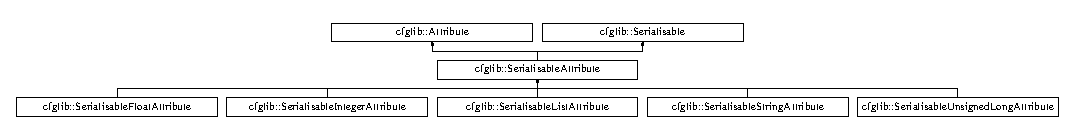
\includegraphics[height=1.344000cm]{classcfglib_1_1SerialisableAttribute}
\end{center}
\end{figure}
\subsection*{Public Member Functions}
\begin{DoxyCompactItemize}
\item 
virtual \hyperlink{classcfglib_1_1SerialisableAttribute}{Serialisable\+Attribute} $\ast$ \hyperlink{classcfglib_1_1SerialisableAttribute_a43e0793a2302b933997b9b3f5156ffff}{create} ()=0
\end{DoxyCompactItemize}
\subsection*{Additional Inherited Members}


\subsection{Detailed Description}
\hyperlink{classcfglib_1_1Attribute}{Attribute} interface. 

\subsection{Member Function Documentation}
\mbox{\Hypertarget{classcfglib_1_1SerialisableAttribute_a43e0793a2302b933997b9b3f5156ffff}\label{classcfglib_1_1SerialisableAttribute_a43e0793a2302b933997b9b3f5156ffff}} 
\index{cfglib\+::\+Serialisable\+Attribute@{cfglib\+::\+Serialisable\+Attribute}!create@{create}}
\index{create@{create}!cfglib\+::\+Serialisable\+Attribute@{cfglib\+::\+Serialisable\+Attribute}}
\subsubsection{\texorpdfstring{create()}{create()}}
{\footnotesize\ttfamily virtual \hyperlink{classcfglib_1_1SerialisableAttribute}{Serialisable\+Attribute}$\ast$ cfglib\+::\+Serialisable\+Attribute\+::create (\begin{DoxyParamCaption}{ }\end{DoxyParamCaption})\hspace{0.3cm}{\ttfamily [pure virtual]}}

Atrribute factory 

Implemented in \hyperlink{classcfglib_1_1SerialisableListAttribute_a00e99bbe0a913edc157e027f9ba9b8f0}{cfglib\+::\+Serialisable\+List\+Attribute}, \hyperlink{classcfglib_1_1SerialisableUnsignedLongAttribute_a394a14fb12e3e0e11f37bf8e625f4901}{cfglib\+::\+Serialisable\+Unsigned\+Long\+Attribute}, \hyperlink{classcfglib_1_1SerialisableFloatAttribute_a47205df866697eb0af48be24f1a0fe5b}{cfglib\+::\+Serialisable\+Float\+Attribute}, \hyperlink{classcfglib_1_1SerialisableIntegerAttribute_ae8b6996fa450b48c0ca1eb79cba008c2}{cfglib\+::\+Serialisable\+Integer\+Attribute}, and \hyperlink{classcfglib_1_1SerialisableStringAttribute_aa9235315d09c87b3ac945ddde53fe85c}{cfglib\+::\+Serialisable\+String\+Attribute}.



The documentation for this class was generated from the following file\+:\begin{DoxyCompactItemize}
\item 
include/\hyperlink{SerialisableAttributes_8h}{Serialisable\+Attributes.\+h}\end{DoxyCompactItemize}

\hypertarget{classcfglib_1_1SerialisableFloatAttribute}{}\section{cfglib\+:\+:Serialisable\+Float\+Attribute Class Reference}
\label{classcfglib_1_1SerialisableFloatAttribute}\index{cfglib\+::\+Serialisable\+Float\+Attribute@{cfglib\+::\+Serialisable\+Float\+Attribute}}


{\ttfamily \#include $<$Serialisable\+Attributes.\+h$>$}

Inheritance diagram for cfglib\+:\+:Serialisable\+Float\+Attribute\+:\begin{figure}[H]
\begin{center}
\leavevmode
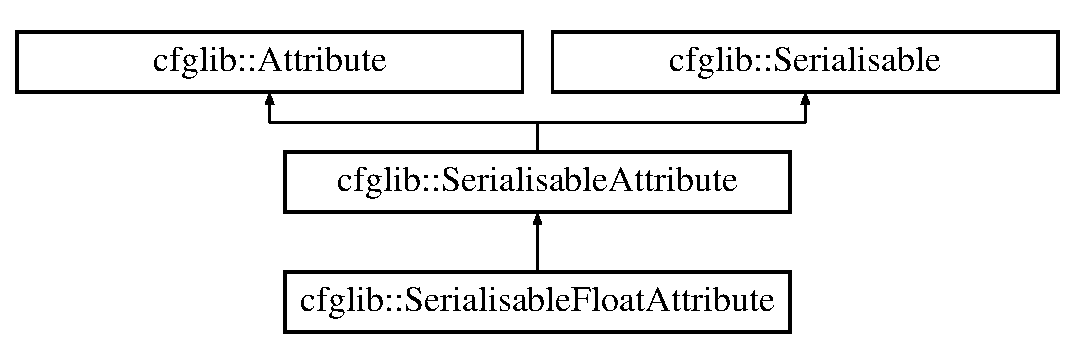
\includegraphics[height=3.000000cm]{classcfglib_1_1SerialisableFloatAttribute}
\end{center}
\end{figure}
\subsection*{Public Member Functions}
\begin{DoxyCompactItemize}
\item 
\hyperlink{classcfglib_1_1SerialisableFloatAttribute_ab6405145d5601d941b9f4d7899e1301e}{Serialisable\+Float\+Attribute} ()
\item 
\hyperlink{classcfglib_1_1SerialisableFloatAttribute_aee912a7511215f8c2308da08f7b852c5}{Serialisable\+Float\+Attribute} (float val)
\item 
\hyperlink{classcfglib_1_1SerialisableFloatAttribute_ab60b6f3fc7ce73b5ad61339fa2466b57}{$\sim$\+Serialisable\+Float\+Attribute} ()
\item 
\hyperlink{classcfglib_1_1SerialisableFloatAttribute}{Serialisable\+Float\+Attribute} $\ast$ \hyperlink{classcfglib_1_1SerialisableFloatAttribute_a2addfc6e4ad308e1e84c2b4cdac7636b}{clone} ()
\item 
void \hyperlink{classcfglib_1_1SerialisableFloatAttribute_af36f296204e1a8547f3fbef7ec4c23da}{Print} (std\+::ostream \&)
\item 
std\+::ostream \& \hyperlink{classcfglib_1_1SerialisableFloatAttribute_a6955df1fc620fa672d29d4e2426a6c89}{Write\+Xml} (std\+::ostream \&, \hyperlink{classcfglib_1_1Handle}{Handle} \&)
\item 
virtual void \hyperlink{classcfglib_1_1SerialisableFloatAttribute_a622fedde5c15cc5fe891d57c932d5355}{Read\+Xml} (\hyperlink{classXmlTag}{Xml\+Tag} const $\ast$, \hyperlink{classcfglib_1_1Handle}{cfglib\+::\+Handle} \&)
\item 
float \hyperlink{classcfglib_1_1SerialisableFloatAttribute_a820299e89405d3c13b300688778e4a85}{Get\+Value} ()
\item 
void \hyperlink{classcfglib_1_1SerialisableFloatAttribute_ae53727839365c40f44883abeaa38c9f5}{Set\+Value} (float v)
\item 
\hyperlink{classcfglib_1_1SerialisableFloatAttribute}{Serialisable\+Float\+Attribute} $\ast$ \hyperlink{classcfglib_1_1SerialisableFloatAttribute_a47205df866697eb0af48be24f1a0fe5b}{create} ()
\end{DoxyCompactItemize}
\subsection*{Additional Inherited Members}


\subsection{Constructor \& Destructor Documentation}
\mbox{\Hypertarget{classcfglib_1_1SerialisableFloatAttribute_ab6405145d5601d941b9f4d7899e1301e}\label{classcfglib_1_1SerialisableFloatAttribute_ab6405145d5601d941b9f4d7899e1301e}} 
\index{cfglib\+::\+Serialisable\+Float\+Attribute@{cfglib\+::\+Serialisable\+Float\+Attribute}!Serialisable\+Float\+Attribute@{Serialisable\+Float\+Attribute}}
\index{Serialisable\+Float\+Attribute@{Serialisable\+Float\+Attribute}!cfglib\+::\+Serialisable\+Float\+Attribute@{cfglib\+::\+Serialisable\+Float\+Attribute}}
\subsubsection{\texorpdfstring{Serialisable\+Float\+Attribute()}{SerialisableFloatAttribute()}\hspace{0.1cm}{\footnotesize\ttfamily [1/2]}}
{\footnotesize\ttfamily cfglib\+::\+Serialisable\+Float\+Attribute\+::\+Serialisable\+Float\+Attribute (\begin{DoxyParamCaption}{ }\end{DoxyParamCaption})\hspace{0.3cm}{\ttfamily [inline]}}

Constructor \mbox{\Hypertarget{classcfglib_1_1SerialisableFloatAttribute_aee912a7511215f8c2308da08f7b852c5}\label{classcfglib_1_1SerialisableFloatAttribute_aee912a7511215f8c2308da08f7b852c5}} 
\index{cfglib\+::\+Serialisable\+Float\+Attribute@{cfglib\+::\+Serialisable\+Float\+Attribute}!Serialisable\+Float\+Attribute@{Serialisable\+Float\+Attribute}}
\index{Serialisable\+Float\+Attribute@{Serialisable\+Float\+Attribute}!cfglib\+::\+Serialisable\+Float\+Attribute@{cfglib\+::\+Serialisable\+Float\+Attribute}}
\subsubsection{\texorpdfstring{Serialisable\+Float\+Attribute()}{SerialisableFloatAttribute()}\hspace{0.1cm}{\footnotesize\ttfamily [2/2]}}
{\footnotesize\ttfamily cfglib\+::\+Serialisable\+Float\+Attribute\+::\+Serialisable\+Float\+Attribute (\begin{DoxyParamCaption}\item[{float}]{val }\end{DoxyParamCaption})\hspace{0.3cm}{\ttfamily [inline]}}

\mbox{\Hypertarget{classcfglib_1_1SerialisableFloatAttribute_ab60b6f3fc7ce73b5ad61339fa2466b57}\label{classcfglib_1_1SerialisableFloatAttribute_ab60b6f3fc7ce73b5ad61339fa2466b57}} 
\index{cfglib\+::\+Serialisable\+Float\+Attribute@{cfglib\+::\+Serialisable\+Float\+Attribute}!````~Serialisable\+Float\+Attribute@{$\sim$\+Serialisable\+Float\+Attribute}}
\index{````~Serialisable\+Float\+Attribute@{$\sim$\+Serialisable\+Float\+Attribute}!cfglib\+::\+Serialisable\+Float\+Attribute@{cfglib\+::\+Serialisable\+Float\+Attribute}}
\subsubsection{\texorpdfstring{$\sim$\+Serialisable\+Float\+Attribute()}{~SerialisableFloatAttribute()}}
{\footnotesize\ttfamily cfglib\+::\+Serialisable\+Float\+Attribute\+::$\sim$\+Serialisable\+Float\+Attribute (\begin{DoxyParamCaption}{ }\end{DoxyParamCaption})\hspace{0.3cm}{\ttfamily [inline]}}

default constructor. 

\subsection{Member Function Documentation}
\mbox{\Hypertarget{classcfglib_1_1SerialisableFloatAttribute_a2addfc6e4ad308e1e84c2b4cdac7636b}\label{classcfglib_1_1SerialisableFloatAttribute_a2addfc6e4ad308e1e84c2b4cdac7636b}} 
\index{cfglib\+::\+Serialisable\+Float\+Attribute@{cfglib\+::\+Serialisable\+Float\+Attribute}!clone@{clone}}
\index{clone@{clone}!cfglib\+::\+Serialisable\+Float\+Attribute@{cfglib\+::\+Serialisable\+Float\+Attribute}}
\subsubsection{\texorpdfstring{clone()}{clone()}}
{\footnotesize\ttfamily \hyperlink{classcfglib_1_1SerialisableFloatAttribute}{Serialisable\+Float\+Attribute}$\ast$ cfglib\+::\+Serialisable\+Float\+Attribute\+::clone (\begin{DoxyParamCaption}{ }\end{DoxyParamCaption})\hspace{0.3cm}{\ttfamily [virtual]}}

virtual constructor 

Implements \hyperlink{classcfglib_1_1Attribute_a107366042fdafe881215426059fec3f8}{cfglib\+::\+Attribute}.

\mbox{\Hypertarget{classcfglib_1_1SerialisableFloatAttribute_a47205df866697eb0af48be24f1a0fe5b}\label{classcfglib_1_1SerialisableFloatAttribute_a47205df866697eb0af48be24f1a0fe5b}} 
\index{cfglib\+::\+Serialisable\+Float\+Attribute@{cfglib\+::\+Serialisable\+Float\+Attribute}!create@{create}}
\index{create@{create}!cfglib\+::\+Serialisable\+Float\+Attribute@{cfglib\+::\+Serialisable\+Float\+Attribute}}
\subsubsection{\texorpdfstring{create()}{create()}}
{\footnotesize\ttfamily \hyperlink{classcfglib_1_1SerialisableFloatAttribute}{Serialisable\+Float\+Attribute}$\ast$ cfglib\+::\+Serialisable\+Float\+Attribute\+::create (\begin{DoxyParamCaption}{ }\end{DoxyParamCaption})\hspace{0.3cm}{\ttfamily [virtual]}}

Factory 

Implements \hyperlink{classcfglib_1_1SerialisableAttribute_a43e0793a2302b933997b9b3f5156ffff}{cfglib\+::\+Serialisable\+Attribute}.

\mbox{\Hypertarget{classcfglib_1_1SerialisableFloatAttribute_a820299e89405d3c13b300688778e4a85}\label{classcfglib_1_1SerialisableFloatAttribute_a820299e89405d3c13b300688778e4a85}} 
\index{cfglib\+::\+Serialisable\+Float\+Attribute@{cfglib\+::\+Serialisable\+Float\+Attribute}!Get\+Value@{Get\+Value}}
\index{Get\+Value@{Get\+Value}!cfglib\+::\+Serialisable\+Float\+Attribute@{cfglib\+::\+Serialisable\+Float\+Attribute}}
\subsubsection{\texorpdfstring{Get\+Value()}{GetValue()}}
{\footnotesize\ttfamily float cfglib\+::\+Serialisable\+Float\+Attribute\+::\+Get\+Value (\begin{DoxyParamCaption}{ }\end{DoxyParamCaption})\hspace{0.3cm}{\ttfamily [inline]}}

get int value of the Integer \hyperlink{classcfglib_1_1Attribute}{Attribute} \mbox{\Hypertarget{classcfglib_1_1SerialisableFloatAttribute_af36f296204e1a8547f3fbef7ec4c23da}\label{classcfglib_1_1SerialisableFloatAttribute_af36f296204e1a8547f3fbef7ec4c23da}} 
\index{cfglib\+::\+Serialisable\+Float\+Attribute@{cfglib\+::\+Serialisable\+Float\+Attribute}!Print@{Print}}
\index{Print@{Print}!cfglib\+::\+Serialisable\+Float\+Attribute@{cfglib\+::\+Serialisable\+Float\+Attribute}}
\subsubsection{\texorpdfstring{Print()}{Print()}}
{\footnotesize\ttfamily void cfglib\+::\+Serialisable\+Float\+Attribute\+::\+Print (\begin{DoxyParamCaption}\item[{std\+::ostream \&}]{ }\end{DoxyParamCaption})\hspace{0.3cm}{\ttfamily [virtual]}}

\hyperlink{classcfglib_1_1Attribute}{Attribute} printing function (debug only) 

Implements \hyperlink{classcfglib_1_1Attribute_af8d87ceddde146b92727e61823e0129b}{cfglib\+::\+Attribute}.

\mbox{\Hypertarget{classcfglib_1_1SerialisableFloatAttribute_a622fedde5c15cc5fe891d57c932d5355}\label{classcfglib_1_1SerialisableFloatAttribute_a622fedde5c15cc5fe891d57c932d5355}} 
\index{cfglib\+::\+Serialisable\+Float\+Attribute@{cfglib\+::\+Serialisable\+Float\+Attribute}!Read\+Xml@{Read\+Xml}}
\index{Read\+Xml@{Read\+Xml}!cfglib\+::\+Serialisable\+Float\+Attribute@{cfglib\+::\+Serialisable\+Float\+Attribute}}
\subsubsection{\texorpdfstring{Read\+Xml()}{ReadXml()}}
{\footnotesize\ttfamily virtual void cfglib\+::\+Serialisable\+Float\+Attribute\+::\+Read\+Xml (\begin{DoxyParamCaption}\item[{\hyperlink{classXmlTag}{Xml\+Tag} const $\ast$}]{,  }\item[{\hyperlink{classcfglib_1_1Handle}{cfglib\+::\+Handle} \&}]{ }\end{DoxyParamCaption})\hspace{0.3cm}{\ttfamily [virtual]}}

deserialisation function 

Implements \hyperlink{classcfglib_1_1Serialisable_a876d530446317872259356af9b016e13}{cfglib\+::\+Serialisable}.

\mbox{\Hypertarget{classcfglib_1_1SerialisableFloatAttribute_ae53727839365c40f44883abeaa38c9f5}\label{classcfglib_1_1SerialisableFloatAttribute_ae53727839365c40f44883abeaa38c9f5}} 
\index{cfglib\+::\+Serialisable\+Float\+Attribute@{cfglib\+::\+Serialisable\+Float\+Attribute}!Set\+Value@{Set\+Value}}
\index{Set\+Value@{Set\+Value}!cfglib\+::\+Serialisable\+Float\+Attribute@{cfglib\+::\+Serialisable\+Float\+Attribute}}
\subsubsection{\texorpdfstring{Set\+Value()}{SetValue()}}
{\footnotesize\ttfamily void cfglib\+::\+Serialisable\+Float\+Attribute\+::\+Set\+Value (\begin{DoxyParamCaption}\item[{float}]{v }\end{DoxyParamCaption})\hspace{0.3cm}{\ttfamily [inline]}}

set the value of the Integer attribute \mbox{\Hypertarget{classcfglib_1_1SerialisableFloatAttribute_a6955df1fc620fa672d29d4e2426a6c89}\label{classcfglib_1_1SerialisableFloatAttribute_a6955df1fc620fa672d29d4e2426a6c89}} 
\index{cfglib\+::\+Serialisable\+Float\+Attribute@{cfglib\+::\+Serialisable\+Float\+Attribute}!Write\+Xml@{Write\+Xml}}
\index{Write\+Xml@{Write\+Xml}!cfglib\+::\+Serialisable\+Float\+Attribute@{cfglib\+::\+Serialisable\+Float\+Attribute}}
\subsubsection{\texorpdfstring{Write\+Xml()}{WriteXml()}}
{\footnotesize\ttfamily std\+::ostream\& cfglib\+::\+Serialisable\+Float\+Attribute\+::\+Write\+Xml (\begin{DoxyParamCaption}\item[{std\+::ostream \&}]{,  }\item[{\hyperlink{classcfglib_1_1Handle}{Handle} \&}]{ }\end{DoxyParamCaption})\hspace{0.3cm}{\ttfamily [virtual]}}

Serialisation function 

Implements \hyperlink{classcfglib_1_1Serialisable_aaeb80cc7397ad312e5ae34f39412ce42}{cfglib\+::\+Serialisable}.



The documentation for this class was generated from the following file\+:\begin{DoxyCompactItemize}
\item 
include/\hyperlink{SerialisableAttributes_8h}{Serialisable\+Attributes.\+h}\end{DoxyCompactItemize}

\hypertarget{classcfglib_1_1SerialisableIntegerAttribute}{}\section{cfglib\+:\+:Serialisable\+Integer\+Attribute Class Reference}
\label{classcfglib_1_1SerialisableIntegerAttribute}\index{cfglib\+::\+Serialisable\+Integer\+Attribute@{cfglib\+::\+Serialisable\+Integer\+Attribute}}


{\ttfamily \#include $<$Serialisable\+Attributes.\+h$>$}

Inheritance diagram for cfglib\+:\+:Serialisable\+Integer\+Attribute\+:\begin{figure}[H]
\begin{center}
\leavevmode
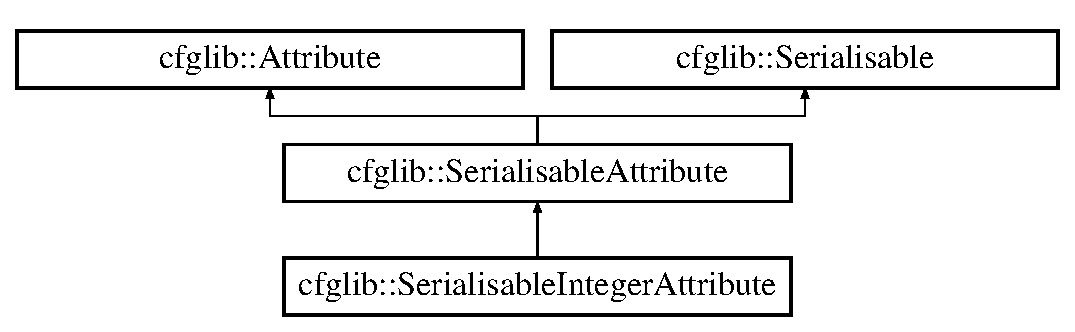
\includegraphics[height=3.000000cm]{classcfglib_1_1SerialisableIntegerAttribute}
\end{center}
\end{figure}
\subsection*{Public Member Functions}
\begin{DoxyCompactItemize}
\item 
\hyperlink{classcfglib_1_1SerialisableIntegerAttribute_a1a5abf78432edf1fd895c00178aa198d}{Serialisable\+Integer\+Attribute} ()
\item 
\hyperlink{classcfglib_1_1SerialisableIntegerAttribute_a93a599cd2519e1b3cfa298aa24aba264}{Serialisable\+Integer\+Attribute} (int val)
\item 
\hyperlink{classcfglib_1_1SerialisableIntegerAttribute_afca7fcb22060b1fca4d4bc2aefe95e01}{$\sim$\+Serialisable\+Integer\+Attribute} ()
\item 
\hyperlink{classcfglib_1_1SerialisableIntegerAttribute}{Serialisable\+Integer\+Attribute} $\ast$ \hyperlink{classcfglib_1_1SerialisableIntegerAttribute_a105ce2b9dab265d56bc3229fcb7d6084}{clone} ()
\item 
void \hyperlink{classcfglib_1_1SerialisableIntegerAttribute_ad2f90817bfc2f4aa2f5be3064e19e11a}{Print} (std\+::ostream \&)
\item 
std\+::ostream \& \hyperlink{classcfglib_1_1SerialisableIntegerAttribute_ac9a38f025a46c97a2030e32f3c5279fa}{Write\+Xml} (std\+::ostream \&, \hyperlink{classcfglib_1_1Handle}{Handle} \&)
\item 
virtual void \hyperlink{classcfglib_1_1SerialisableIntegerAttribute_ab1a2955d8dc60ee2a23e819c1f9d4386}{Read\+Xml} (\hyperlink{classXmlTag}{Xml\+Tag} const $\ast$, \hyperlink{classcfglib_1_1Handle}{cfglib\+::\+Handle} \&)
\item 
int \hyperlink{classcfglib_1_1SerialisableIntegerAttribute_aa554b851238bb27153713ae48f5f7701}{Get\+Value} ()
\item 
void \hyperlink{classcfglib_1_1SerialisableIntegerAttribute_a23ec7f33655351cbe5121978ac67db46}{Set\+Value} (int v)
\item 
\hyperlink{classcfglib_1_1SerialisableIntegerAttribute}{Serialisable\+Integer\+Attribute} $\ast$ \hyperlink{classcfglib_1_1SerialisableIntegerAttribute_ae8b6996fa450b48c0ca1eb79cba008c2}{create} ()
\end{DoxyCompactItemize}
\subsection*{Additional Inherited Members}


\subsection{Constructor \& Destructor Documentation}
\mbox{\Hypertarget{classcfglib_1_1SerialisableIntegerAttribute_a1a5abf78432edf1fd895c00178aa198d}\label{classcfglib_1_1SerialisableIntegerAttribute_a1a5abf78432edf1fd895c00178aa198d}} 
\index{cfglib\+::\+Serialisable\+Integer\+Attribute@{cfglib\+::\+Serialisable\+Integer\+Attribute}!Serialisable\+Integer\+Attribute@{Serialisable\+Integer\+Attribute}}
\index{Serialisable\+Integer\+Attribute@{Serialisable\+Integer\+Attribute}!cfglib\+::\+Serialisable\+Integer\+Attribute@{cfglib\+::\+Serialisable\+Integer\+Attribute}}
\subsubsection{\texorpdfstring{Serialisable\+Integer\+Attribute()}{SerialisableIntegerAttribute()}\hspace{0.1cm}{\footnotesize\ttfamily [1/2]}}
{\footnotesize\ttfamily cfglib\+::\+Serialisable\+Integer\+Attribute\+::\+Serialisable\+Integer\+Attribute (\begin{DoxyParamCaption}{ }\end{DoxyParamCaption})\hspace{0.3cm}{\ttfamily [inline]}}

Constructor \mbox{\Hypertarget{classcfglib_1_1SerialisableIntegerAttribute_a93a599cd2519e1b3cfa298aa24aba264}\label{classcfglib_1_1SerialisableIntegerAttribute_a93a599cd2519e1b3cfa298aa24aba264}} 
\index{cfglib\+::\+Serialisable\+Integer\+Attribute@{cfglib\+::\+Serialisable\+Integer\+Attribute}!Serialisable\+Integer\+Attribute@{Serialisable\+Integer\+Attribute}}
\index{Serialisable\+Integer\+Attribute@{Serialisable\+Integer\+Attribute}!cfglib\+::\+Serialisable\+Integer\+Attribute@{cfglib\+::\+Serialisable\+Integer\+Attribute}}
\subsubsection{\texorpdfstring{Serialisable\+Integer\+Attribute()}{SerialisableIntegerAttribute()}\hspace{0.1cm}{\footnotesize\ttfamily [2/2]}}
{\footnotesize\ttfamily cfglib\+::\+Serialisable\+Integer\+Attribute\+::\+Serialisable\+Integer\+Attribute (\begin{DoxyParamCaption}\item[{int}]{val }\end{DoxyParamCaption})\hspace{0.3cm}{\ttfamily [inline]}}

\mbox{\Hypertarget{classcfglib_1_1SerialisableIntegerAttribute_afca7fcb22060b1fca4d4bc2aefe95e01}\label{classcfglib_1_1SerialisableIntegerAttribute_afca7fcb22060b1fca4d4bc2aefe95e01}} 
\index{cfglib\+::\+Serialisable\+Integer\+Attribute@{cfglib\+::\+Serialisable\+Integer\+Attribute}!````~Serialisable\+Integer\+Attribute@{$\sim$\+Serialisable\+Integer\+Attribute}}
\index{````~Serialisable\+Integer\+Attribute@{$\sim$\+Serialisable\+Integer\+Attribute}!cfglib\+::\+Serialisable\+Integer\+Attribute@{cfglib\+::\+Serialisable\+Integer\+Attribute}}
\subsubsection{\texorpdfstring{$\sim$\+Serialisable\+Integer\+Attribute()}{~SerialisableIntegerAttribute()}}
{\footnotesize\ttfamily cfglib\+::\+Serialisable\+Integer\+Attribute\+::$\sim$\+Serialisable\+Integer\+Attribute (\begin{DoxyParamCaption}{ }\end{DoxyParamCaption})\hspace{0.3cm}{\ttfamily [inline]}}

default constructor. 

\subsection{Member Function Documentation}
\mbox{\Hypertarget{classcfglib_1_1SerialisableIntegerAttribute_a105ce2b9dab265d56bc3229fcb7d6084}\label{classcfglib_1_1SerialisableIntegerAttribute_a105ce2b9dab265d56bc3229fcb7d6084}} 
\index{cfglib\+::\+Serialisable\+Integer\+Attribute@{cfglib\+::\+Serialisable\+Integer\+Attribute}!clone@{clone}}
\index{clone@{clone}!cfglib\+::\+Serialisable\+Integer\+Attribute@{cfglib\+::\+Serialisable\+Integer\+Attribute}}
\subsubsection{\texorpdfstring{clone()}{clone()}}
{\footnotesize\ttfamily \hyperlink{classcfglib_1_1SerialisableIntegerAttribute}{Serialisable\+Integer\+Attribute}$\ast$ cfglib\+::\+Serialisable\+Integer\+Attribute\+::clone (\begin{DoxyParamCaption}{ }\end{DoxyParamCaption})\hspace{0.3cm}{\ttfamily [virtual]}}

virtual constructor 

Implements \hyperlink{classcfglib_1_1Attribute_a107366042fdafe881215426059fec3f8}{cfglib\+::\+Attribute}.

\mbox{\Hypertarget{classcfglib_1_1SerialisableIntegerAttribute_ae8b6996fa450b48c0ca1eb79cba008c2}\label{classcfglib_1_1SerialisableIntegerAttribute_ae8b6996fa450b48c0ca1eb79cba008c2}} 
\index{cfglib\+::\+Serialisable\+Integer\+Attribute@{cfglib\+::\+Serialisable\+Integer\+Attribute}!create@{create}}
\index{create@{create}!cfglib\+::\+Serialisable\+Integer\+Attribute@{cfglib\+::\+Serialisable\+Integer\+Attribute}}
\subsubsection{\texorpdfstring{create()}{create()}}
{\footnotesize\ttfamily \hyperlink{classcfglib_1_1SerialisableIntegerAttribute}{Serialisable\+Integer\+Attribute}$\ast$ cfglib\+::\+Serialisable\+Integer\+Attribute\+::create (\begin{DoxyParamCaption}{ }\end{DoxyParamCaption})\hspace{0.3cm}{\ttfamily [virtual]}}

Factory 

Implements \hyperlink{classcfglib_1_1SerialisableAttribute_a43e0793a2302b933997b9b3f5156ffff}{cfglib\+::\+Serialisable\+Attribute}.

\mbox{\Hypertarget{classcfglib_1_1SerialisableIntegerAttribute_aa554b851238bb27153713ae48f5f7701}\label{classcfglib_1_1SerialisableIntegerAttribute_aa554b851238bb27153713ae48f5f7701}} 
\index{cfglib\+::\+Serialisable\+Integer\+Attribute@{cfglib\+::\+Serialisable\+Integer\+Attribute}!Get\+Value@{Get\+Value}}
\index{Get\+Value@{Get\+Value}!cfglib\+::\+Serialisable\+Integer\+Attribute@{cfglib\+::\+Serialisable\+Integer\+Attribute}}
\subsubsection{\texorpdfstring{Get\+Value()}{GetValue()}}
{\footnotesize\ttfamily int cfglib\+::\+Serialisable\+Integer\+Attribute\+::\+Get\+Value (\begin{DoxyParamCaption}{ }\end{DoxyParamCaption})\hspace{0.3cm}{\ttfamily [inline]}}

get int value of the Integer \hyperlink{classcfglib_1_1Attribute}{Attribute} \mbox{\Hypertarget{classcfglib_1_1SerialisableIntegerAttribute_ad2f90817bfc2f4aa2f5be3064e19e11a}\label{classcfglib_1_1SerialisableIntegerAttribute_ad2f90817bfc2f4aa2f5be3064e19e11a}} 
\index{cfglib\+::\+Serialisable\+Integer\+Attribute@{cfglib\+::\+Serialisable\+Integer\+Attribute}!Print@{Print}}
\index{Print@{Print}!cfglib\+::\+Serialisable\+Integer\+Attribute@{cfglib\+::\+Serialisable\+Integer\+Attribute}}
\subsubsection{\texorpdfstring{Print()}{Print()}}
{\footnotesize\ttfamily void cfglib\+::\+Serialisable\+Integer\+Attribute\+::\+Print (\begin{DoxyParamCaption}\item[{std\+::ostream \&}]{ }\end{DoxyParamCaption})\hspace{0.3cm}{\ttfamily [virtual]}}

\hyperlink{classcfglib_1_1Attribute}{Attribute} printing function (debug only) 

Implements \hyperlink{classcfglib_1_1Attribute_af8d87ceddde146b92727e61823e0129b}{cfglib\+::\+Attribute}.

\mbox{\Hypertarget{classcfglib_1_1SerialisableIntegerAttribute_ab1a2955d8dc60ee2a23e819c1f9d4386}\label{classcfglib_1_1SerialisableIntegerAttribute_ab1a2955d8dc60ee2a23e819c1f9d4386}} 
\index{cfglib\+::\+Serialisable\+Integer\+Attribute@{cfglib\+::\+Serialisable\+Integer\+Attribute}!Read\+Xml@{Read\+Xml}}
\index{Read\+Xml@{Read\+Xml}!cfglib\+::\+Serialisable\+Integer\+Attribute@{cfglib\+::\+Serialisable\+Integer\+Attribute}}
\subsubsection{\texorpdfstring{Read\+Xml()}{ReadXml()}}
{\footnotesize\ttfamily virtual void cfglib\+::\+Serialisable\+Integer\+Attribute\+::\+Read\+Xml (\begin{DoxyParamCaption}\item[{\hyperlink{classXmlTag}{Xml\+Tag} const $\ast$}]{,  }\item[{\hyperlink{classcfglib_1_1Handle}{cfglib\+::\+Handle} \&}]{ }\end{DoxyParamCaption})\hspace{0.3cm}{\ttfamily [virtual]}}

deserialisation function 

Implements \hyperlink{classcfglib_1_1Serialisable_a876d530446317872259356af9b016e13}{cfglib\+::\+Serialisable}.

\mbox{\Hypertarget{classcfglib_1_1SerialisableIntegerAttribute_a23ec7f33655351cbe5121978ac67db46}\label{classcfglib_1_1SerialisableIntegerAttribute_a23ec7f33655351cbe5121978ac67db46}} 
\index{cfglib\+::\+Serialisable\+Integer\+Attribute@{cfglib\+::\+Serialisable\+Integer\+Attribute}!Set\+Value@{Set\+Value}}
\index{Set\+Value@{Set\+Value}!cfglib\+::\+Serialisable\+Integer\+Attribute@{cfglib\+::\+Serialisable\+Integer\+Attribute}}
\subsubsection{\texorpdfstring{Set\+Value()}{SetValue()}}
{\footnotesize\ttfamily void cfglib\+::\+Serialisable\+Integer\+Attribute\+::\+Set\+Value (\begin{DoxyParamCaption}\item[{int}]{v }\end{DoxyParamCaption})\hspace{0.3cm}{\ttfamily [inline]}}

set the value of the Integer attribute \mbox{\Hypertarget{classcfglib_1_1SerialisableIntegerAttribute_ac9a38f025a46c97a2030e32f3c5279fa}\label{classcfglib_1_1SerialisableIntegerAttribute_ac9a38f025a46c97a2030e32f3c5279fa}} 
\index{cfglib\+::\+Serialisable\+Integer\+Attribute@{cfglib\+::\+Serialisable\+Integer\+Attribute}!Write\+Xml@{Write\+Xml}}
\index{Write\+Xml@{Write\+Xml}!cfglib\+::\+Serialisable\+Integer\+Attribute@{cfglib\+::\+Serialisable\+Integer\+Attribute}}
\subsubsection{\texorpdfstring{Write\+Xml()}{WriteXml()}}
{\footnotesize\ttfamily std\+::ostream\& cfglib\+::\+Serialisable\+Integer\+Attribute\+::\+Write\+Xml (\begin{DoxyParamCaption}\item[{std\+::ostream \&}]{,  }\item[{\hyperlink{classcfglib_1_1Handle}{Handle} \&}]{ }\end{DoxyParamCaption})\hspace{0.3cm}{\ttfamily [virtual]}}

Serialisation function 

Implements \hyperlink{classcfglib_1_1Serialisable_aaeb80cc7397ad312e5ae34f39412ce42}{cfglib\+::\+Serialisable}.



The documentation for this class was generated from the following file\+:\begin{DoxyCompactItemize}
\item 
include/\hyperlink{SerialisableAttributes_8h}{Serialisable\+Attributes.\+h}\end{DoxyCompactItemize}

\hypertarget{classcfglib_1_1SerialisableListAttribute}{}\section{cfglib\+:\+:Serialisable\+List\+Attribute Class Reference}
\label{classcfglib_1_1SerialisableListAttribute}\index{cfglib\+::\+Serialisable\+List\+Attribute@{cfglib\+::\+Serialisable\+List\+Attribute}}


{\ttfamily \#include $<$Serialisable\+Attributes.\+h$>$}

Inheritance diagram for cfglib\+:\+:Serialisable\+List\+Attribute\+:\begin{figure}[H]
\begin{center}
\leavevmode
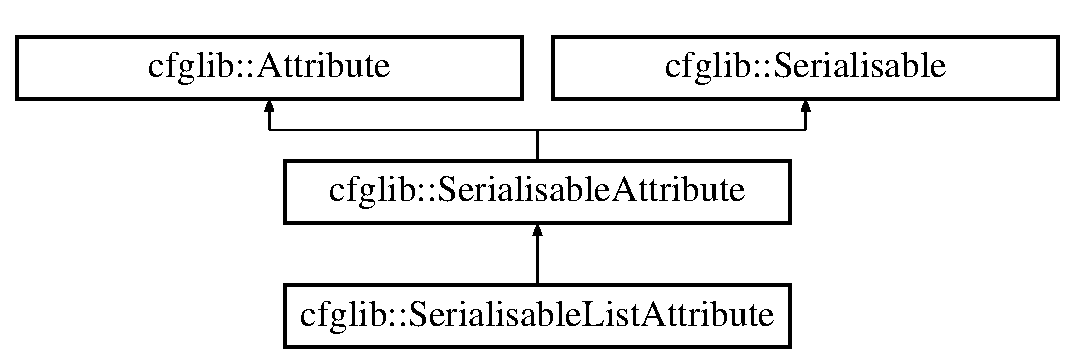
\includegraphics[height=3.000000cm]{classcfglib_1_1SerialisableListAttribute}
\end{center}
\end{figure}
\subsection*{Public Member Functions}
\begin{DoxyCompactItemize}
\item 
\hyperlink{classcfglib_1_1SerialisableListAttribute_a5952feba3ff71af2b1dc71d176d4b541}{Serialisable\+List\+Attribute} ()
\item 
\hyperlink{classcfglib_1_1SerialisableListAttribute_ac00d97a9d6f778a5ef70938807e17225}{Serialisable\+List\+Attribute} (\hyperlink{classcfglib_1_1SerialisableListAttribute}{Serialisable\+List\+Attribute} \&v)
\item 
\hyperlink{classcfglib_1_1SerialisableListAttribute_ab4fee35259518cd7223dc59a80fd8e8c}{Serialisable\+List\+Attribute} (list$<$ \hyperlink{classcfglib_1_1SerialisableAttribute}{Serialisable\+Attribute} $\ast$$>$ l)
\item 
\hyperlink{classcfglib_1_1SerialisableListAttribute_a375c9b6e54d8c1e4c12538d944ddb594}{$\sim$\+Serialisable\+List\+Attribute} ()
\item 
\hyperlink{classcfglib_1_1SerialisableListAttribute}{Serialisable\+List\+Attribute} $\ast$ \hyperlink{classcfglib_1_1SerialisableListAttribute_a8fe3db52648fbc4d6f08a4bdf7c78ea6}{clone} ()
\item 
\hyperlink{classcfglib_1_1SerialisableListAttribute}{Serialisable\+List\+Attribute} $\ast$ \hyperlink{classcfglib_1_1SerialisableListAttribute_a2bcd8907e26992e725a8a10b82288a0f}{clone} (\hyperlink{classcfglib_1_1CloneHandle}{Clone\+Handle} \&handle)
\item 
void \hyperlink{classcfglib_1_1SerialisableListAttribute_a3a76c800c9ebcd084b64c1c5f049caf5}{Print} (std\+::ostream \&)
\item 
std\+::ostream \& \hyperlink{classcfglib_1_1SerialisableListAttribute_a9e407c7a002d8ec7ed0b934842380736}{Write\+Xml} (std\+::ostream \&, \hyperlink{classcfglib_1_1Handle}{Handle} \&)
\item 
virtual void \hyperlink{classcfglib_1_1SerialisableListAttribute_a70350e44db8c97a8abfcf2d6bce82151}{Read\+Xml} (\hyperlink{classXmlTag}{Xml\+Tag} const $\ast$, \hyperlink{classcfglib_1_1Handle}{cfglib\+::\+Handle} \&)
\item 
list$<$ \hyperlink{classcfglib_1_1SerialisableAttribute}{Serialisable\+Attribute} $\ast$ $>$ \hyperlink{classcfglib_1_1SerialisableListAttribute_af8534bcf974bc68717fe369059b45146}{Get\+Value} ()
\item 
void \hyperlink{classcfglib_1_1SerialisableListAttribute_a0f6a00fb09fe4cbc2a875dc021201f02}{Set\+Value} (list$<$ \hyperlink{classcfglib_1_1SerialisableAttribute}{Serialisable\+Attribute} $\ast$$>$ v)
\item 
\hyperlink{classcfglib_1_1SerialisableListAttribute}{Serialisable\+List\+Attribute} $\ast$ \hyperlink{classcfglib_1_1SerialisableListAttribute_a00e99bbe0a913edc157e027f9ba9b8f0}{create} ()
\end{DoxyCompactItemize}
\subsection*{Additional Inherited Members}


\subsection{Constructor \& Destructor Documentation}
\mbox{\Hypertarget{classcfglib_1_1SerialisableListAttribute_a5952feba3ff71af2b1dc71d176d4b541}\label{classcfglib_1_1SerialisableListAttribute_a5952feba3ff71af2b1dc71d176d4b541}} 
\index{cfglib\+::\+Serialisable\+List\+Attribute@{cfglib\+::\+Serialisable\+List\+Attribute}!Serialisable\+List\+Attribute@{Serialisable\+List\+Attribute}}
\index{Serialisable\+List\+Attribute@{Serialisable\+List\+Attribute}!cfglib\+::\+Serialisable\+List\+Attribute@{cfglib\+::\+Serialisable\+List\+Attribute}}
\subsubsection{\texorpdfstring{Serialisable\+List\+Attribute()}{SerialisableListAttribute()}\hspace{0.1cm}{\footnotesize\ttfamily [1/3]}}
{\footnotesize\ttfamily cfglib\+::\+Serialisable\+List\+Attribute\+::\+Serialisable\+List\+Attribute (\begin{DoxyParamCaption}{ }\end{DoxyParamCaption})\hspace{0.3cm}{\ttfamily [inline]}}

Constructor \mbox{\Hypertarget{classcfglib_1_1SerialisableListAttribute_ac00d97a9d6f778a5ef70938807e17225}\label{classcfglib_1_1SerialisableListAttribute_ac00d97a9d6f778a5ef70938807e17225}} 
\index{cfglib\+::\+Serialisable\+List\+Attribute@{cfglib\+::\+Serialisable\+List\+Attribute}!Serialisable\+List\+Attribute@{Serialisable\+List\+Attribute}}
\index{Serialisable\+List\+Attribute@{Serialisable\+List\+Attribute}!cfglib\+::\+Serialisable\+List\+Attribute@{cfglib\+::\+Serialisable\+List\+Attribute}}
\subsubsection{\texorpdfstring{Serialisable\+List\+Attribute()}{SerialisableListAttribute()}\hspace{0.1cm}{\footnotesize\ttfamily [2/3]}}
{\footnotesize\ttfamily cfglib\+::\+Serialisable\+List\+Attribute\+::\+Serialisable\+List\+Attribute (\begin{DoxyParamCaption}\item[{\hyperlink{classcfglib_1_1SerialisableListAttribute}{Serialisable\+List\+Attribute} \&}]{v }\end{DoxyParamCaption})}

\mbox{\Hypertarget{classcfglib_1_1SerialisableListAttribute_ab4fee35259518cd7223dc59a80fd8e8c}\label{classcfglib_1_1SerialisableListAttribute_ab4fee35259518cd7223dc59a80fd8e8c}} 
\index{cfglib\+::\+Serialisable\+List\+Attribute@{cfglib\+::\+Serialisable\+List\+Attribute}!Serialisable\+List\+Attribute@{Serialisable\+List\+Attribute}}
\index{Serialisable\+List\+Attribute@{Serialisable\+List\+Attribute}!cfglib\+::\+Serialisable\+List\+Attribute@{cfglib\+::\+Serialisable\+List\+Attribute}}
\subsubsection{\texorpdfstring{Serialisable\+List\+Attribute()}{SerialisableListAttribute()}\hspace{0.1cm}{\footnotesize\ttfamily [3/3]}}
{\footnotesize\ttfamily cfglib\+::\+Serialisable\+List\+Attribute\+::\+Serialisable\+List\+Attribute (\begin{DoxyParamCaption}\item[{list$<$ \hyperlink{classcfglib_1_1SerialisableAttribute}{Serialisable\+Attribute} $\ast$$>$}]{l }\end{DoxyParamCaption})\hspace{0.3cm}{\ttfamily [inline]}}

\mbox{\Hypertarget{classcfglib_1_1SerialisableListAttribute_a375c9b6e54d8c1e4c12538d944ddb594}\label{classcfglib_1_1SerialisableListAttribute_a375c9b6e54d8c1e4c12538d944ddb594}} 
\index{cfglib\+::\+Serialisable\+List\+Attribute@{cfglib\+::\+Serialisable\+List\+Attribute}!````~Serialisable\+List\+Attribute@{$\sim$\+Serialisable\+List\+Attribute}}
\index{````~Serialisable\+List\+Attribute@{$\sim$\+Serialisable\+List\+Attribute}!cfglib\+::\+Serialisable\+List\+Attribute@{cfglib\+::\+Serialisable\+List\+Attribute}}
\subsubsection{\texorpdfstring{$\sim$\+Serialisable\+List\+Attribute()}{~SerialisableListAttribute()}}
{\footnotesize\ttfamily cfglib\+::\+Serialisable\+List\+Attribute\+::$\sim$\+Serialisable\+List\+Attribute (\begin{DoxyParamCaption}{ }\end{DoxyParamCaption})\hspace{0.3cm}{\ttfamily [inline]}}

default constructor. 

\subsection{Member Function Documentation}
\mbox{\Hypertarget{classcfglib_1_1SerialisableListAttribute_a8fe3db52648fbc4d6f08a4bdf7c78ea6}\label{classcfglib_1_1SerialisableListAttribute_a8fe3db52648fbc4d6f08a4bdf7c78ea6}} 
\index{cfglib\+::\+Serialisable\+List\+Attribute@{cfglib\+::\+Serialisable\+List\+Attribute}!clone@{clone}}
\index{clone@{clone}!cfglib\+::\+Serialisable\+List\+Attribute@{cfglib\+::\+Serialisable\+List\+Attribute}}
\subsubsection{\texorpdfstring{clone()}{clone()}\hspace{0.1cm}{\footnotesize\ttfamily [1/2]}}
{\footnotesize\ttfamily \hyperlink{classcfglib_1_1SerialisableListAttribute}{Serialisable\+List\+Attribute}$\ast$ cfglib\+::\+Serialisable\+List\+Attribute\+::clone (\begin{DoxyParamCaption}{ }\end{DoxyParamCaption})\hspace{0.3cm}{\ttfamily [virtual]}}

virtual constructor 

Implements \hyperlink{classcfglib_1_1Attribute_a107366042fdafe881215426059fec3f8}{cfglib\+::\+Attribute}.

\mbox{\Hypertarget{classcfglib_1_1SerialisableListAttribute_a2bcd8907e26992e725a8a10b82288a0f}\label{classcfglib_1_1SerialisableListAttribute_a2bcd8907e26992e725a8a10b82288a0f}} 
\index{cfglib\+::\+Serialisable\+List\+Attribute@{cfglib\+::\+Serialisable\+List\+Attribute}!clone@{clone}}
\index{clone@{clone}!cfglib\+::\+Serialisable\+List\+Attribute@{cfglib\+::\+Serialisable\+List\+Attribute}}
\subsubsection{\texorpdfstring{clone()}{clone()}\hspace{0.1cm}{\footnotesize\ttfamily [2/2]}}
{\footnotesize\ttfamily \hyperlink{classcfglib_1_1SerialisableListAttribute}{Serialisable\+List\+Attribute}$\ast$ cfglib\+::\+Serialisable\+List\+Attribute\+::clone (\begin{DoxyParamCaption}\item[{\hyperlink{classcfglib_1_1CloneHandle}{Clone\+Handle} \&}]{handle }\end{DoxyParamCaption})\hspace{0.3cm}{\ttfamily [virtual]}}



Reimplemented from \hyperlink{classcfglib_1_1Attribute_a73490b82f9b31d8f30b813a2a9d3fe99}{cfglib\+::\+Attribute}.

\mbox{\Hypertarget{classcfglib_1_1SerialisableListAttribute_a00e99bbe0a913edc157e027f9ba9b8f0}\label{classcfglib_1_1SerialisableListAttribute_a00e99bbe0a913edc157e027f9ba9b8f0}} 
\index{cfglib\+::\+Serialisable\+List\+Attribute@{cfglib\+::\+Serialisable\+List\+Attribute}!create@{create}}
\index{create@{create}!cfglib\+::\+Serialisable\+List\+Attribute@{cfglib\+::\+Serialisable\+List\+Attribute}}
\subsubsection{\texorpdfstring{create()}{create()}}
{\footnotesize\ttfamily \hyperlink{classcfglib_1_1SerialisableListAttribute}{Serialisable\+List\+Attribute}$\ast$ cfglib\+::\+Serialisable\+List\+Attribute\+::create (\begin{DoxyParamCaption}{ }\end{DoxyParamCaption})\hspace{0.3cm}{\ttfamily [virtual]}}

Factory 

Implements \hyperlink{classcfglib_1_1SerialisableAttribute_a43e0793a2302b933997b9b3f5156ffff}{cfglib\+::\+Serialisable\+Attribute}.

\mbox{\Hypertarget{classcfglib_1_1SerialisableListAttribute_af8534bcf974bc68717fe369059b45146}\label{classcfglib_1_1SerialisableListAttribute_af8534bcf974bc68717fe369059b45146}} 
\index{cfglib\+::\+Serialisable\+List\+Attribute@{cfglib\+::\+Serialisable\+List\+Attribute}!Get\+Value@{Get\+Value}}
\index{Get\+Value@{Get\+Value}!cfglib\+::\+Serialisable\+List\+Attribute@{cfglib\+::\+Serialisable\+List\+Attribute}}
\subsubsection{\texorpdfstring{Get\+Value()}{GetValue()}}
{\footnotesize\ttfamily list$<$\hyperlink{classcfglib_1_1SerialisableAttribute}{Serialisable\+Attribute}$\ast$$>$ cfglib\+::\+Serialisable\+List\+Attribute\+::\+Get\+Value (\begin{DoxyParamCaption}{ }\end{DoxyParamCaption})\hspace{0.3cm}{\ttfamily [inline]}}

get int value of the Serialisable\+List \hyperlink{classcfglib_1_1Attribute}{Attribute} \mbox{\Hypertarget{classcfglib_1_1SerialisableListAttribute_a3a76c800c9ebcd084b64c1c5f049caf5}\label{classcfglib_1_1SerialisableListAttribute_a3a76c800c9ebcd084b64c1c5f049caf5}} 
\index{cfglib\+::\+Serialisable\+List\+Attribute@{cfglib\+::\+Serialisable\+List\+Attribute}!Print@{Print}}
\index{Print@{Print}!cfglib\+::\+Serialisable\+List\+Attribute@{cfglib\+::\+Serialisable\+List\+Attribute}}
\subsubsection{\texorpdfstring{Print()}{Print()}}
{\footnotesize\ttfamily void cfglib\+::\+Serialisable\+List\+Attribute\+::\+Print (\begin{DoxyParamCaption}\item[{std\+::ostream \&}]{ }\end{DoxyParamCaption})\hspace{0.3cm}{\ttfamily [virtual]}}

\hyperlink{classcfglib_1_1Attribute}{Attribute} printing function (debug only) 

Implements \hyperlink{classcfglib_1_1Attribute_af8d87ceddde146b92727e61823e0129b}{cfglib\+::\+Attribute}.

\mbox{\Hypertarget{classcfglib_1_1SerialisableListAttribute_a70350e44db8c97a8abfcf2d6bce82151}\label{classcfglib_1_1SerialisableListAttribute_a70350e44db8c97a8abfcf2d6bce82151}} 
\index{cfglib\+::\+Serialisable\+List\+Attribute@{cfglib\+::\+Serialisable\+List\+Attribute}!Read\+Xml@{Read\+Xml}}
\index{Read\+Xml@{Read\+Xml}!cfglib\+::\+Serialisable\+List\+Attribute@{cfglib\+::\+Serialisable\+List\+Attribute}}
\subsubsection{\texorpdfstring{Read\+Xml()}{ReadXml()}}
{\footnotesize\ttfamily virtual void cfglib\+::\+Serialisable\+List\+Attribute\+::\+Read\+Xml (\begin{DoxyParamCaption}\item[{\hyperlink{classXmlTag}{Xml\+Tag} const $\ast$}]{,  }\item[{\hyperlink{classcfglib_1_1Handle}{cfglib\+::\+Handle} \&}]{ }\end{DoxyParamCaption})\hspace{0.3cm}{\ttfamily [virtual]}}

deserialisation function 

Implements \hyperlink{classcfglib_1_1Serialisable_a876d530446317872259356af9b016e13}{cfglib\+::\+Serialisable}.

\mbox{\Hypertarget{classcfglib_1_1SerialisableListAttribute_a0f6a00fb09fe4cbc2a875dc021201f02}\label{classcfglib_1_1SerialisableListAttribute_a0f6a00fb09fe4cbc2a875dc021201f02}} 
\index{cfglib\+::\+Serialisable\+List\+Attribute@{cfglib\+::\+Serialisable\+List\+Attribute}!Set\+Value@{Set\+Value}}
\index{Set\+Value@{Set\+Value}!cfglib\+::\+Serialisable\+List\+Attribute@{cfglib\+::\+Serialisable\+List\+Attribute}}
\subsubsection{\texorpdfstring{Set\+Value()}{SetValue()}}
{\footnotesize\ttfamily void cfglib\+::\+Serialisable\+List\+Attribute\+::\+Set\+Value (\begin{DoxyParamCaption}\item[{list$<$ \hyperlink{classcfglib_1_1SerialisableAttribute}{Serialisable\+Attribute} $\ast$$>$}]{v }\end{DoxyParamCaption})\hspace{0.3cm}{\ttfamily [inline]}}

set the value of the Serialisable\+List attribute \mbox{\Hypertarget{classcfglib_1_1SerialisableListAttribute_a9e407c7a002d8ec7ed0b934842380736}\label{classcfglib_1_1SerialisableListAttribute_a9e407c7a002d8ec7ed0b934842380736}} 
\index{cfglib\+::\+Serialisable\+List\+Attribute@{cfglib\+::\+Serialisable\+List\+Attribute}!Write\+Xml@{Write\+Xml}}
\index{Write\+Xml@{Write\+Xml}!cfglib\+::\+Serialisable\+List\+Attribute@{cfglib\+::\+Serialisable\+List\+Attribute}}
\subsubsection{\texorpdfstring{Write\+Xml()}{WriteXml()}}
{\footnotesize\ttfamily std\+::ostream\& cfglib\+::\+Serialisable\+List\+Attribute\+::\+Write\+Xml (\begin{DoxyParamCaption}\item[{std\+::ostream \&}]{,  }\item[{\hyperlink{classcfglib_1_1Handle}{Handle} \&}]{ }\end{DoxyParamCaption})\hspace{0.3cm}{\ttfamily [virtual]}}

Serialisation function 

Implements \hyperlink{classcfglib_1_1Serialisable_aaeb80cc7397ad312e5ae34f39412ce42}{cfglib\+::\+Serialisable}.



The documentation for this class was generated from the following file\+:\begin{DoxyCompactItemize}
\item 
include/\hyperlink{SerialisableAttributes_8h}{Serialisable\+Attributes.\+h}\end{DoxyCompactItemize}

\hypertarget{classcfglib_1_1SerialisableStringAttribute}{}\section{cfglib\+:\+:Serialisable\+String\+Attribute Class Reference}
\label{classcfglib_1_1SerialisableStringAttribute}\index{cfglib\+::\+Serialisable\+String\+Attribute@{cfglib\+::\+Serialisable\+String\+Attribute}}


{\ttfamily \#include $<$Serialisable\+Attributes.\+h$>$}

Inheritance diagram for cfglib\+:\+:Serialisable\+String\+Attribute\+:\begin{figure}[H]
\begin{center}
\leavevmode
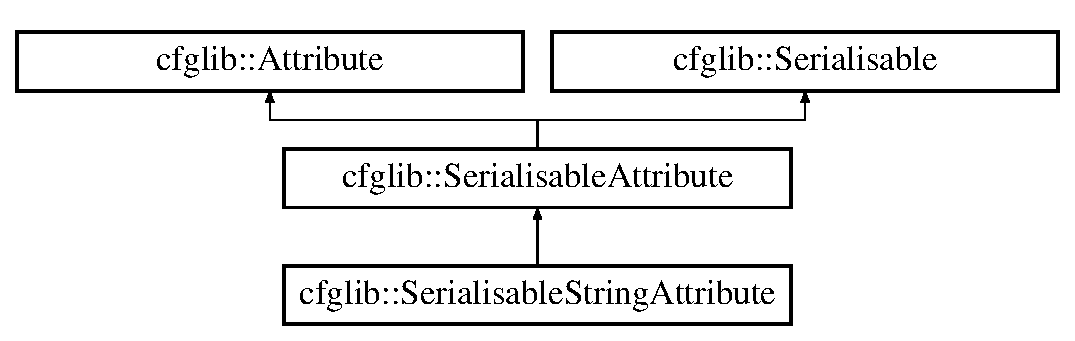
\includegraphics[height=3.000000cm]{classcfglib_1_1SerialisableStringAttribute}
\end{center}
\end{figure}
\subsection*{Public Member Functions}
\begin{DoxyCompactItemize}
\item 
\hyperlink{classcfglib_1_1SerialisableStringAttribute_a1b3dd845194091ebd803f88a36a8ac64}{Serialisable\+String\+Attribute} ()
\item 
\hyperlink{classcfglib_1_1SerialisableStringAttribute_a6d63152ea3ce76cf7efe4529eded7c14}{Serialisable\+String\+Attribute} (std\+::string const \&val)
\item 
\hyperlink{classcfglib_1_1SerialisableStringAttribute_a0dcb908722c68595d0962ee55fc4b92f}{$\sim$\+Serialisable\+String\+Attribute} ()
\item 
virtual \hyperlink{classcfglib_1_1SerialisableStringAttribute}{Serialisable\+String\+Attribute} $\ast$ \hyperlink{classcfglib_1_1SerialisableStringAttribute_a8c1e4b8b3edbb39c85216d2b2cf8ec38}{clone} ()
\item 
void \hyperlink{classcfglib_1_1SerialisableStringAttribute_a7149bb6d92d50db794bde6867cef4550}{Print} (std\+::ostream \&)
\item 
std\+::ostream \& \hyperlink{classcfglib_1_1SerialisableStringAttribute_a25ca4cd51b9acd75e7c75640028e2310}{Write\+Xml} (std\+::ostream \&, \hyperlink{classcfglib_1_1Handle}{Handle} \&)
\item 
virtual void \hyperlink{classcfglib_1_1SerialisableStringAttribute_aa001915e6a54ea8549b4e44da4cade74}{Read\+Xml} (\hyperlink{classXmlTag}{Xml\+Tag} const $\ast$, \hyperlink{classcfglib_1_1Handle}{cfglib\+::\+Handle} \&)
\item 
std\+::string \hyperlink{classcfglib_1_1SerialisableStringAttribute_af03bc94771d0997eb1a78f05b6f763a9}{Get\+Value} ()
\item 
void \hyperlink{classcfglib_1_1SerialisableStringAttribute_acb99eee7e7ab298a0fc425ca956edd31}{Set\+Value} (std\+::string v)
\item 
\hyperlink{classcfglib_1_1SerialisableStringAttribute}{Serialisable\+String\+Attribute} $\ast$ \hyperlink{classcfglib_1_1SerialisableStringAttribute_aa9235315d09c87b3ac945ddde53fe85c}{create} ()
\end{DoxyCompactItemize}
\subsection*{Additional Inherited Members}


\subsection{Constructor \& Destructor Documentation}
\mbox{\Hypertarget{classcfglib_1_1SerialisableStringAttribute_a1b3dd845194091ebd803f88a36a8ac64}\label{classcfglib_1_1SerialisableStringAttribute_a1b3dd845194091ebd803f88a36a8ac64}} 
\index{cfglib\+::\+Serialisable\+String\+Attribute@{cfglib\+::\+Serialisable\+String\+Attribute}!Serialisable\+String\+Attribute@{Serialisable\+String\+Attribute}}
\index{Serialisable\+String\+Attribute@{Serialisable\+String\+Attribute}!cfglib\+::\+Serialisable\+String\+Attribute@{cfglib\+::\+Serialisable\+String\+Attribute}}
\subsubsection{\texorpdfstring{Serialisable\+String\+Attribute()}{SerialisableStringAttribute()}\hspace{0.1cm}{\footnotesize\ttfamily [1/2]}}
{\footnotesize\ttfamily cfglib\+::\+Serialisable\+String\+Attribute\+::\+Serialisable\+String\+Attribute (\begin{DoxyParamCaption}{ }\end{DoxyParamCaption})\hspace{0.3cm}{\ttfamily [inline]}}

Constructor \mbox{\Hypertarget{classcfglib_1_1SerialisableStringAttribute_a6d63152ea3ce76cf7efe4529eded7c14}\label{classcfglib_1_1SerialisableStringAttribute_a6d63152ea3ce76cf7efe4529eded7c14}} 
\index{cfglib\+::\+Serialisable\+String\+Attribute@{cfglib\+::\+Serialisable\+String\+Attribute}!Serialisable\+String\+Attribute@{Serialisable\+String\+Attribute}}
\index{Serialisable\+String\+Attribute@{Serialisable\+String\+Attribute}!cfglib\+::\+Serialisable\+String\+Attribute@{cfglib\+::\+Serialisable\+String\+Attribute}}
\subsubsection{\texorpdfstring{Serialisable\+String\+Attribute()}{SerialisableStringAttribute()}\hspace{0.1cm}{\footnotesize\ttfamily [2/2]}}
{\footnotesize\ttfamily cfglib\+::\+Serialisable\+String\+Attribute\+::\+Serialisable\+String\+Attribute (\begin{DoxyParamCaption}\item[{std\+::string const \&}]{val }\end{DoxyParamCaption})\hspace{0.3cm}{\ttfamily [inline]}}

\mbox{\Hypertarget{classcfglib_1_1SerialisableStringAttribute_a0dcb908722c68595d0962ee55fc4b92f}\label{classcfglib_1_1SerialisableStringAttribute_a0dcb908722c68595d0962ee55fc4b92f}} 
\index{cfglib\+::\+Serialisable\+String\+Attribute@{cfglib\+::\+Serialisable\+String\+Attribute}!````~Serialisable\+String\+Attribute@{$\sim$\+Serialisable\+String\+Attribute}}
\index{````~Serialisable\+String\+Attribute@{$\sim$\+Serialisable\+String\+Attribute}!cfglib\+::\+Serialisable\+String\+Attribute@{cfglib\+::\+Serialisable\+String\+Attribute}}
\subsubsection{\texorpdfstring{$\sim$\+Serialisable\+String\+Attribute()}{~SerialisableStringAttribute()}}
{\footnotesize\ttfamily cfglib\+::\+Serialisable\+String\+Attribute\+::$\sim$\+Serialisable\+String\+Attribute (\begin{DoxyParamCaption}{ }\end{DoxyParamCaption})\hspace{0.3cm}{\ttfamily [inline]}}

default constructor. 

\subsection{Member Function Documentation}
\mbox{\Hypertarget{classcfglib_1_1SerialisableStringAttribute_a8c1e4b8b3edbb39c85216d2b2cf8ec38}\label{classcfglib_1_1SerialisableStringAttribute_a8c1e4b8b3edbb39c85216d2b2cf8ec38}} 
\index{cfglib\+::\+Serialisable\+String\+Attribute@{cfglib\+::\+Serialisable\+String\+Attribute}!clone@{clone}}
\index{clone@{clone}!cfglib\+::\+Serialisable\+String\+Attribute@{cfglib\+::\+Serialisable\+String\+Attribute}}
\subsubsection{\texorpdfstring{clone()}{clone()}}
{\footnotesize\ttfamily virtual \hyperlink{classcfglib_1_1SerialisableStringAttribute}{Serialisable\+String\+Attribute}$\ast$ cfglib\+::\+Serialisable\+String\+Attribute\+::clone (\begin{DoxyParamCaption}{ }\end{DoxyParamCaption})\hspace{0.3cm}{\ttfamily [virtual]}}

virtual constructor 

Implements \hyperlink{classcfglib_1_1Attribute_a107366042fdafe881215426059fec3f8}{cfglib\+::\+Attribute}.

\mbox{\Hypertarget{classcfglib_1_1SerialisableStringAttribute_aa9235315d09c87b3ac945ddde53fe85c}\label{classcfglib_1_1SerialisableStringAttribute_aa9235315d09c87b3ac945ddde53fe85c}} 
\index{cfglib\+::\+Serialisable\+String\+Attribute@{cfglib\+::\+Serialisable\+String\+Attribute}!create@{create}}
\index{create@{create}!cfglib\+::\+Serialisable\+String\+Attribute@{cfglib\+::\+Serialisable\+String\+Attribute}}
\subsubsection{\texorpdfstring{create()}{create()}}
{\footnotesize\ttfamily \hyperlink{classcfglib_1_1SerialisableStringAttribute}{Serialisable\+String\+Attribute}$\ast$ cfglib\+::\+Serialisable\+String\+Attribute\+::create (\begin{DoxyParamCaption}{ }\end{DoxyParamCaption})\hspace{0.3cm}{\ttfamily [virtual]}}

Factory 

Implements \hyperlink{classcfglib_1_1SerialisableAttribute_a43e0793a2302b933997b9b3f5156ffff}{cfglib\+::\+Serialisable\+Attribute}.

\mbox{\Hypertarget{classcfglib_1_1SerialisableStringAttribute_af03bc94771d0997eb1a78f05b6f763a9}\label{classcfglib_1_1SerialisableStringAttribute_af03bc94771d0997eb1a78f05b6f763a9}} 
\index{cfglib\+::\+Serialisable\+String\+Attribute@{cfglib\+::\+Serialisable\+String\+Attribute}!Get\+Value@{Get\+Value}}
\index{Get\+Value@{Get\+Value}!cfglib\+::\+Serialisable\+String\+Attribute@{cfglib\+::\+Serialisable\+String\+Attribute}}
\subsubsection{\texorpdfstring{Get\+Value()}{GetValue()}}
{\footnotesize\ttfamily std\+::string cfglib\+::\+Serialisable\+String\+Attribute\+::\+Get\+Value (\begin{DoxyParamCaption}{ }\end{DoxyParamCaption})\hspace{0.3cm}{\ttfamily [inline]}}

get std\+::string value of the String \hyperlink{classcfglib_1_1Attribute}{Attribute} \mbox{\Hypertarget{classcfglib_1_1SerialisableStringAttribute_a7149bb6d92d50db794bde6867cef4550}\label{classcfglib_1_1SerialisableStringAttribute_a7149bb6d92d50db794bde6867cef4550}} 
\index{cfglib\+::\+Serialisable\+String\+Attribute@{cfglib\+::\+Serialisable\+String\+Attribute}!Print@{Print}}
\index{Print@{Print}!cfglib\+::\+Serialisable\+String\+Attribute@{cfglib\+::\+Serialisable\+String\+Attribute}}
\subsubsection{\texorpdfstring{Print()}{Print()}}
{\footnotesize\ttfamily void cfglib\+::\+Serialisable\+String\+Attribute\+::\+Print (\begin{DoxyParamCaption}\item[{std\+::ostream \&}]{ }\end{DoxyParamCaption})\hspace{0.3cm}{\ttfamily [virtual]}}

\hyperlink{classcfglib_1_1Attribute}{Attribute} printing function (debug only) 

Implements \hyperlink{classcfglib_1_1Attribute_af8d87ceddde146b92727e61823e0129b}{cfglib\+::\+Attribute}.

\mbox{\Hypertarget{classcfglib_1_1SerialisableStringAttribute_aa001915e6a54ea8549b4e44da4cade74}\label{classcfglib_1_1SerialisableStringAttribute_aa001915e6a54ea8549b4e44da4cade74}} 
\index{cfglib\+::\+Serialisable\+String\+Attribute@{cfglib\+::\+Serialisable\+String\+Attribute}!Read\+Xml@{Read\+Xml}}
\index{Read\+Xml@{Read\+Xml}!cfglib\+::\+Serialisable\+String\+Attribute@{cfglib\+::\+Serialisable\+String\+Attribute}}
\subsubsection{\texorpdfstring{Read\+Xml()}{ReadXml()}}
{\footnotesize\ttfamily virtual void cfglib\+::\+Serialisable\+String\+Attribute\+::\+Read\+Xml (\begin{DoxyParamCaption}\item[{\hyperlink{classXmlTag}{Xml\+Tag} const $\ast$}]{,  }\item[{\hyperlink{classcfglib_1_1Handle}{cfglib\+::\+Handle} \&}]{ }\end{DoxyParamCaption})\hspace{0.3cm}{\ttfamily [virtual]}}

deserialisation function 

Implements \hyperlink{classcfglib_1_1Serialisable_a876d530446317872259356af9b016e13}{cfglib\+::\+Serialisable}.

\mbox{\Hypertarget{classcfglib_1_1SerialisableStringAttribute_acb99eee7e7ab298a0fc425ca956edd31}\label{classcfglib_1_1SerialisableStringAttribute_acb99eee7e7ab298a0fc425ca956edd31}} 
\index{cfglib\+::\+Serialisable\+String\+Attribute@{cfglib\+::\+Serialisable\+String\+Attribute}!Set\+Value@{Set\+Value}}
\index{Set\+Value@{Set\+Value}!cfglib\+::\+Serialisable\+String\+Attribute@{cfglib\+::\+Serialisable\+String\+Attribute}}
\subsubsection{\texorpdfstring{Set\+Value()}{SetValue()}}
{\footnotesize\ttfamily void cfglib\+::\+Serialisable\+String\+Attribute\+::\+Set\+Value (\begin{DoxyParamCaption}\item[{std\+::string}]{v }\end{DoxyParamCaption})\hspace{0.3cm}{\ttfamily [inline]}}

set the value of the String attribute \mbox{\Hypertarget{classcfglib_1_1SerialisableStringAttribute_a25ca4cd51b9acd75e7c75640028e2310}\label{classcfglib_1_1SerialisableStringAttribute_a25ca4cd51b9acd75e7c75640028e2310}} 
\index{cfglib\+::\+Serialisable\+String\+Attribute@{cfglib\+::\+Serialisable\+String\+Attribute}!Write\+Xml@{Write\+Xml}}
\index{Write\+Xml@{Write\+Xml}!cfglib\+::\+Serialisable\+String\+Attribute@{cfglib\+::\+Serialisable\+String\+Attribute}}
\subsubsection{\texorpdfstring{Write\+Xml()}{WriteXml()}}
{\footnotesize\ttfamily std\+::ostream\& cfglib\+::\+Serialisable\+String\+Attribute\+::\+Write\+Xml (\begin{DoxyParamCaption}\item[{std\+::ostream \&}]{,  }\item[{\hyperlink{classcfglib_1_1Handle}{Handle} \&}]{ }\end{DoxyParamCaption})\hspace{0.3cm}{\ttfamily [virtual]}}

Serialisation function 

Implements \hyperlink{classcfglib_1_1Serialisable_aaeb80cc7397ad312e5ae34f39412ce42}{cfglib\+::\+Serialisable}.



The documentation for this class was generated from the following file\+:\begin{DoxyCompactItemize}
\item 
include/\hyperlink{SerialisableAttributes_8h}{Serialisable\+Attributes.\+h}\end{DoxyCompactItemize}

\hypertarget{classcfglib_1_1SerialisableUnsignedLongAttribute}{}\section{cfglib\+:\+:Serialisable\+Unsigned\+Long\+Attribute Class Reference}
\label{classcfglib_1_1SerialisableUnsignedLongAttribute}\index{cfglib\+::\+Serialisable\+Unsigned\+Long\+Attribute@{cfglib\+::\+Serialisable\+Unsigned\+Long\+Attribute}}


{\ttfamily \#include $<$Serialisable\+Attributes.\+h$>$}

Inheritance diagram for cfglib\+:\+:Serialisable\+Unsigned\+Long\+Attribute\+:\begin{figure}[H]
\begin{center}
\leavevmode
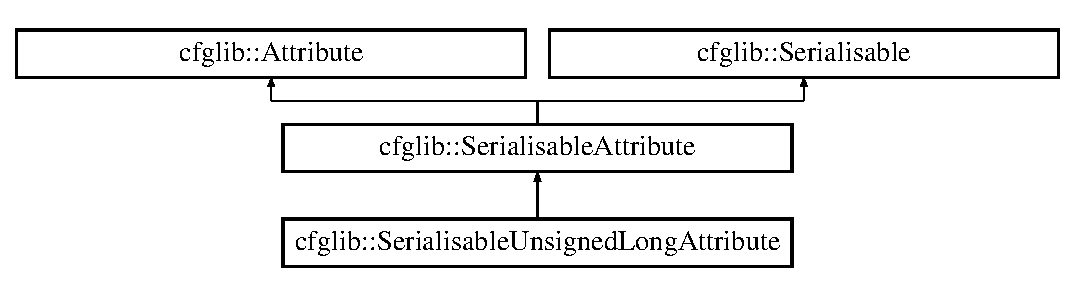
\includegraphics[height=3.000000cm]{classcfglib_1_1SerialisableUnsignedLongAttribute}
\end{center}
\end{figure}
\subsection*{Public Member Functions}
\begin{DoxyCompactItemize}
\item 
\hyperlink{classcfglib_1_1SerialisableUnsignedLongAttribute_aff224e279f182410e70cc2f73dc38f26}{Serialisable\+Unsigned\+Long\+Attribute} ()
\item 
\hyperlink{classcfglib_1_1SerialisableUnsignedLongAttribute_ac6880388351a7c03d870af88e4f06091}{Serialisable\+Unsigned\+Long\+Attribute} (unsigned long val)
\item 
\hyperlink{classcfglib_1_1SerialisableUnsignedLongAttribute_a7b2c594072846372117bd1f3add92a55}{$\sim$\+Serialisable\+Unsigned\+Long\+Attribute} ()
\item 
\hyperlink{classcfglib_1_1SerialisableUnsignedLongAttribute}{Serialisable\+Unsigned\+Long\+Attribute} $\ast$ \hyperlink{classcfglib_1_1SerialisableUnsignedLongAttribute_a5ddcd35aa3f13ae354bf6dd65839baba}{clone} ()
\item 
void \hyperlink{classcfglib_1_1SerialisableUnsignedLongAttribute_a4d53682ce58f689045c6f55a04e1c6cd}{Print} (std\+::ostream \&)
\item 
std\+::ostream \& \hyperlink{classcfglib_1_1SerialisableUnsignedLongAttribute_ad0ffd60cbd393da8b75508c14ab43ce2}{Write\+Xml} (std\+::ostream \&, \hyperlink{classcfglib_1_1Handle}{Handle} \&)
\item 
virtual void \hyperlink{classcfglib_1_1SerialisableUnsignedLongAttribute_acbd51f33a309bb606b7182ab0d49463b}{Read\+Xml} (\hyperlink{classXmlTag}{Xml\+Tag} const $\ast$, \hyperlink{classcfglib_1_1Handle}{cfglib\+::\+Handle} \&)
\item 
unsigned long \hyperlink{classcfglib_1_1SerialisableUnsignedLongAttribute_a185de3958143579ecdef682cafda4ae8}{Get\+Value} ()
\item 
void \hyperlink{classcfglib_1_1SerialisableUnsignedLongAttribute_a9d6e44a34c15ede16bfb85bd3b817990}{Set\+Value} (unsigned long v)
\item 
\hyperlink{classcfglib_1_1SerialisableUnsignedLongAttribute}{Serialisable\+Unsigned\+Long\+Attribute} $\ast$ \hyperlink{classcfglib_1_1SerialisableUnsignedLongAttribute_a394a14fb12e3e0e11f37bf8e625f4901}{create} ()
\end{DoxyCompactItemize}
\subsection*{Additional Inherited Members}


\subsection{Constructor \& Destructor Documentation}
\mbox{\Hypertarget{classcfglib_1_1SerialisableUnsignedLongAttribute_aff224e279f182410e70cc2f73dc38f26}\label{classcfglib_1_1SerialisableUnsignedLongAttribute_aff224e279f182410e70cc2f73dc38f26}} 
\index{cfglib\+::\+Serialisable\+Unsigned\+Long\+Attribute@{cfglib\+::\+Serialisable\+Unsigned\+Long\+Attribute}!Serialisable\+Unsigned\+Long\+Attribute@{Serialisable\+Unsigned\+Long\+Attribute}}
\index{Serialisable\+Unsigned\+Long\+Attribute@{Serialisable\+Unsigned\+Long\+Attribute}!cfglib\+::\+Serialisable\+Unsigned\+Long\+Attribute@{cfglib\+::\+Serialisable\+Unsigned\+Long\+Attribute}}
\subsubsection{\texorpdfstring{Serialisable\+Unsigned\+Long\+Attribute()}{SerialisableUnsignedLongAttribute()}\hspace{0.1cm}{\footnotesize\ttfamily [1/2]}}
{\footnotesize\ttfamily cfglib\+::\+Serialisable\+Unsigned\+Long\+Attribute\+::\+Serialisable\+Unsigned\+Long\+Attribute (\begin{DoxyParamCaption}{ }\end{DoxyParamCaption})\hspace{0.3cm}{\ttfamily [inline]}}

Constructor \mbox{\Hypertarget{classcfglib_1_1SerialisableUnsignedLongAttribute_ac6880388351a7c03d870af88e4f06091}\label{classcfglib_1_1SerialisableUnsignedLongAttribute_ac6880388351a7c03d870af88e4f06091}} 
\index{cfglib\+::\+Serialisable\+Unsigned\+Long\+Attribute@{cfglib\+::\+Serialisable\+Unsigned\+Long\+Attribute}!Serialisable\+Unsigned\+Long\+Attribute@{Serialisable\+Unsigned\+Long\+Attribute}}
\index{Serialisable\+Unsigned\+Long\+Attribute@{Serialisable\+Unsigned\+Long\+Attribute}!cfglib\+::\+Serialisable\+Unsigned\+Long\+Attribute@{cfglib\+::\+Serialisable\+Unsigned\+Long\+Attribute}}
\subsubsection{\texorpdfstring{Serialisable\+Unsigned\+Long\+Attribute()}{SerialisableUnsignedLongAttribute()}\hspace{0.1cm}{\footnotesize\ttfamily [2/2]}}
{\footnotesize\ttfamily cfglib\+::\+Serialisable\+Unsigned\+Long\+Attribute\+::\+Serialisable\+Unsigned\+Long\+Attribute (\begin{DoxyParamCaption}\item[{unsigned long}]{val }\end{DoxyParamCaption})\hspace{0.3cm}{\ttfamily [inline]}}

\mbox{\Hypertarget{classcfglib_1_1SerialisableUnsignedLongAttribute_a7b2c594072846372117bd1f3add92a55}\label{classcfglib_1_1SerialisableUnsignedLongAttribute_a7b2c594072846372117bd1f3add92a55}} 
\index{cfglib\+::\+Serialisable\+Unsigned\+Long\+Attribute@{cfglib\+::\+Serialisable\+Unsigned\+Long\+Attribute}!````~Serialisable\+Unsigned\+Long\+Attribute@{$\sim$\+Serialisable\+Unsigned\+Long\+Attribute}}
\index{````~Serialisable\+Unsigned\+Long\+Attribute@{$\sim$\+Serialisable\+Unsigned\+Long\+Attribute}!cfglib\+::\+Serialisable\+Unsigned\+Long\+Attribute@{cfglib\+::\+Serialisable\+Unsigned\+Long\+Attribute}}
\subsubsection{\texorpdfstring{$\sim$\+Serialisable\+Unsigned\+Long\+Attribute()}{~SerialisableUnsignedLongAttribute()}}
{\footnotesize\ttfamily cfglib\+::\+Serialisable\+Unsigned\+Long\+Attribute\+::$\sim$\+Serialisable\+Unsigned\+Long\+Attribute (\begin{DoxyParamCaption}{ }\end{DoxyParamCaption})\hspace{0.3cm}{\ttfamily [inline]}}

default constructor. 

\subsection{Member Function Documentation}
\mbox{\Hypertarget{classcfglib_1_1SerialisableUnsignedLongAttribute_a5ddcd35aa3f13ae354bf6dd65839baba}\label{classcfglib_1_1SerialisableUnsignedLongAttribute_a5ddcd35aa3f13ae354bf6dd65839baba}} 
\index{cfglib\+::\+Serialisable\+Unsigned\+Long\+Attribute@{cfglib\+::\+Serialisable\+Unsigned\+Long\+Attribute}!clone@{clone}}
\index{clone@{clone}!cfglib\+::\+Serialisable\+Unsigned\+Long\+Attribute@{cfglib\+::\+Serialisable\+Unsigned\+Long\+Attribute}}
\subsubsection{\texorpdfstring{clone()}{clone()}}
{\footnotesize\ttfamily \hyperlink{classcfglib_1_1SerialisableUnsignedLongAttribute}{Serialisable\+Unsigned\+Long\+Attribute}$\ast$ cfglib\+::\+Serialisable\+Unsigned\+Long\+Attribute\+::clone (\begin{DoxyParamCaption}{ }\end{DoxyParamCaption})\hspace{0.3cm}{\ttfamily [virtual]}}

cloning function 

Implements \hyperlink{classcfglib_1_1Attribute_a107366042fdafe881215426059fec3f8}{cfglib\+::\+Attribute}.

\mbox{\Hypertarget{classcfglib_1_1SerialisableUnsignedLongAttribute_a394a14fb12e3e0e11f37bf8e625f4901}\label{classcfglib_1_1SerialisableUnsignedLongAttribute_a394a14fb12e3e0e11f37bf8e625f4901}} 
\index{cfglib\+::\+Serialisable\+Unsigned\+Long\+Attribute@{cfglib\+::\+Serialisable\+Unsigned\+Long\+Attribute}!create@{create}}
\index{create@{create}!cfglib\+::\+Serialisable\+Unsigned\+Long\+Attribute@{cfglib\+::\+Serialisable\+Unsigned\+Long\+Attribute}}
\subsubsection{\texorpdfstring{create()}{create()}}
{\footnotesize\ttfamily \hyperlink{classcfglib_1_1SerialisableUnsignedLongAttribute}{Serialisable\+Unsigned\+Long\+Attribute}$\ast$ cfglib\+::\+Serialisable\+Unsigned\+Long\+Attribute\+::create (\begin{DoxyParamCaption}{ }\end{DoxyParamCaption})\hspace{0.3cm}{\ttfamily [virtual]}}

Factory 

Implements \hyperlink{classcfglib_1_1SerialisableAttribute_a43e0793a2302b933997b9b3f5156ffff}{cfglib\+::\+Serialisable\+Attribute}.

\mbox{\Hypertarget{classcfglib_1_1SerialisableUnsignedLongAttribute_a185de3958143579ecdef682cafda4ae8}\label{classcfglib_1_1SerialisableUnsignedLongAttribute_a185de3958143579ecdef682cafda4ae8}} 
\index{cfglib\+::\+Serialisable\+Unsigned\+Long\+Attribute@{cfglib\+::\+Serialisable\+Unsigned\+Long\+Attribute}!Get\+Value@{Get\+Value}}
\index{Get\+Value@{Get\+Value}!cfglib\+::\+Serialisable\+Unsigned\+Long\+Attribute@{cfglib\+::\+Serialisable\+Unsigned\+Long\+Attribute}}
\subsubsection{\texorpdfstring{Get\+Value()}{GetValue()}}
{\footnotesize\ttfamily unsigned long cfglib\+::\+Serialisable\+Unsigned\+Long\+Attribute\+::\+Get\+Value (\begin{DoxyParamCaption}{ }\end{DoxyParamCaption})\hspace{0.3cm}{\ttfamily [inline]}}

get int value of the Unsigned\+Long \hyperlink{classcfglib_1_1Attribute}{Attribute} \mbox{\Hypertarget{classcfglib_1_1SerialisableUnsignedLongAttribute_a4d53682ce58f689045c6f55a04e1c6cd}\label{classcfglib_1_1SerialisableUnsignedLongAttribute_a4d53682ce58f689045c6f55a04e1c6cd}} 
\index{cfglib\+::\+Serialisable\+Unsigned\+Long\+Attribute@{cfglib\+::\+Serialisable\+Unsigned\+Long\+Attribute}!Print@{Print}}
\index{Print@{Print}!cfglib\+::\+Serialisable\+Unsigned\+Long\+Attribute@{cfglib\+::\+Serialisable\+Unsigned\+Long\+Attribute}}
\subsubsection{\texorpdfstring{Print()}{Print()}}
{\footnotesize\ttfamily void cfglib\+::\+Serialisable\+Unsigned\+Long\+Attribute\+::\+Print (\begin{DoxyParamCaption}\item[{std\+::ostream \&}]{ }\end{DoxyParamCaption})\hspace{0.3cm}{\ttfamily [virtual]}}

\hyperlink{classcfglib_1_1Attribute}{Attribute} printing function (debug only) 

Implements \hyperlink{classcfglib_1_1Attribute_af8d87ceddde146b92727e61823e0129b}{cfglib\+::\+Attribute}.

\mbox{\Hypertarget{classcfglib_1_1SerialisableUnsignedLongAttribute_acbd51f33a309bb606b7182ab0d49463b}\label{classcfglib_1_1SerialisableUnsignedLongAttribute_acbd51f33a309bb606b7182ab0d49463b}} 
\index{cfglib\+::\+Serialisable\+Unsigned\+Long\+Attribute@{cfglib\+::\+Serialisable\+Unsigned\+Long\+Attribute}!Read\+Xml@{Read\+Xml}}
\index{Read\+Xml@{Read\+Xml}!cfglib\+::\+Serialisable\+Unsigned\+Long\+Attribute@{cfglib\+::\+Serialisable\+Unsigned\+Long\+Attribute}}
\subsubsection{\texorpdfstring{Read\+Xml()}{ReadXml()}}
{\footnotesize\ttfamily virtual void cfglib\+::\+Serialisable\+Unsigned\+Long\+Attribute\+::\+Read\+Xml (\begin{DoxyParamCaption}\item[{\hyperlink{classXmlTag}{Xml\+Tag} const $\ast$}]{,  }\item[{\hyperlink{classcfglib_1_1Handle}{cfglib\+::\+Handle} \&}]{ }\end{DoxyParamCaption})\hspace{0.3cm}{\ttfamily [virtual]}}

deserialisation function 

Implements \hyperlink{classcfglib_1_1Serialisable_a876d530446317872259356af9b016e13}{cfglib\+::\+Serialisable}.

\mbox{\Hypertarget{classcfglib_1_1SerialisableUnsignedLongAttribute_a9d6e44a34c15ede16bfb85bd3b817990}\label{classcfglib_1_1SerialisableUnsignedLongAttribute_a9d6e44a34c15ede16bfb85bd3b817990}} 
\index{cfglib\+::\+Serialisable\+Unsigned\+Long\+Attribute@{cfglib\+::\+Serialisable\+Unsigned\+Long\+Attribute}!Set\+Value@{Set\+Value}}
\index{Set\+Value@{Set\+Value}!cfglib\+::\+Serialisable\+Unsigned\+Long\+Attribute@{cfglib\+::\+Serialisable\+Unsigned\+Long\+Attribute}}
\subsubsection{\texorpdfstring{Set\+Value()}{SetValue()}}
{\footnotesize\ttfamily void cfglib\+::\+Serialisable\+Unsigned\+Long\+Attribute\+::\+Set\+Value (\begin{DoxyParamCaption}\item[{unsigned long}]{v }\end{DoxyParamCaption})\hspace{0.3cm}{\ttfamily [inline]}}

set the value of the Unsigned\+Long \hyperlink{classcfglib_1_1Attribute}{Attribute} \mbox{\Hypertarget{classcfglib_1_1SerialisableUnsignedLongAttribute_ad0ffd60cbd393da8b75508c14ab43ce2}\label{classcfglib_1_1SerialisableUnsignedLongAttribute_ad0ffd60cbd393da8b75508c14ab43ce2}} 
\index{cfglib\+::\+Serialisable\+Unsigned\+Long\+Attribute@{cfglib\+::\+Serialisable\+Unsigned\+Long\+Attribute}!Write\+Xml@{Write\+Xml}}
\index{Write\+Xml@{Write\+Xml}!cfglib\+::\+Serialisable\+Unsigned\+Long\+Attribute@{cfglib\+::\+Serialisable\+Unsigned\+Long\+Attribute}}
\subsubsection{\texorpdfstring{Write\+Xml()}{WriteXml()}}
{\footnotesize\ttfamily std\+::ostream\& cfglib\+::\+Serialisable\+Unsigned\+Long\+Attribute\+::\+Write\+Xml (\begin{DoxyParamCaption}\item[{std\+::ostream \&}]{,  }\item[{\hyperlink{classcfglib_1_1Handle}{Handle} \&}]{ }\end{DoxyParamCaption})\hspace{0.3cm}{\ttfamily [virtual]}}

Serialisation function 

Implements \hyperlink{classcfglib_1_1Serialisable_aaeb80cc7397ad312e5ae34f39412ce42}{cfglib\+::\+Serialisable}.



The documentation for this class was generated from the following file\+:\begin{DoxyCompactItemize}
\item 
include/\hyperlink{SerialisableAttributes_8h}{Serialisable\+Attributes.\+h}\end{DoxyCompactItemize}

\hypertarget{classXmlDocument}{}\section{Xml\+Document Class Reference}
\label{classXmlDocument}\index{Xml\+Document@{Xml\+Document}}


{\ttfamily \#include $<$Xml\+Extra.\+h$>$}

\subsection*{Public Member Functions}
\begin{DoxyCompactItemize}
\item 
\hyperlink{classXmlDocument_a0e61a2b4d61602d3aa9c09e8916913e5}{Xml\+Document} (string)
\item 
int \hyperlink{classXmlDocument_ae8f7f34abeaac2ba755a71b9d12ff7b6}{open\+Document} (string)
\item 
\hyperlink{classXmlDocument_ab18742228f580a5e4ec87e4b39c8a68c}{$\sim$\+Xml\+Document} ()
\item 
\hyperlink{XmlExtra_8h_ade6a1aa0dc76b2c26a120f5c2f10ff7d}{List\+Xml\+Tag} \hyperlink{classXmlDocument_a79bce84756484b2026ee7fd15ba61b08}{search\+Children} (string children\+Name)
\item 
\hyperlink{classXmlTag}{Xml\+Tag} \hyperlink{classXmlDocument_a9c8b12f61097276eb79e31672fd30efe}{get\+Root\+Tag} ()
\end{DoxyCompactItemize}


\subsection{Detailed Description}
An X\+ML document to handle\+: opening, closing, get the first children tags 

\subsection{Constructor \& Destructor Documentation}
\mbox{\Hypertarget{classXmlDocument_a0e61a2b4d61602d3aa9c09e8916913e5}\label{classXmlDocument_a0e61a2b4d61602d3aa9c09e8916913e5}} 
\index{Xml\+Document@{Xml\+Document}!Xml\+Document@{Xml\+Document}}
\index{Xml\+Document@{Xml\+Document}!Xml\+Document@{Xml\+Document}}
\subsubsection{\texorpdfstring{Xml\+Document()}{XmlDocument()}}
{\footnotesize\ttfamily Xml\+Document\+::\+Xml\+Document (\begin{DoxyParamCaption}\item[{string}]{ }\end{DoxyParamCaption})}

opening a file, whose name is given \mbox{\Hypertarget{classXmlDocument_ab18742228f580a5e4ec87e4b39c8a68c}\label{classXmlDocument_ab18742228f580a5e4ec87e4b39c8a68c}} 
\index{Xml\+Document@{Xml\+Document}!````~Xml\+Document@{$\sim$\+Xml\+Document}}
\index{````~Xml\+Document@{$\sim$\+Xml\+Document}!Xml\+Document@{Xml\+Document}}
\subsubsection{\texorpdfstring{$\sim$\+Xml\+Document()}{~XmlDocument()}}
{\footnotesize\ttfamily Xml\+Document\+::$\sim$\+Xml\+Document (\begin{DoxyParamCaption}{ }\end{DoxyParamCaption})}

Close document. 

\subsection{Member Function Documentation}
\mbox{\Hypertarget{classXmlDocument_a9c8b12f61097276eb79e31672fd30efe}\label{classXmlDocument_a9c8b12f61097276eb79e31672fd30efe}} 
\index{Xml\+Document@{Xml\+Document}!get\+Root\+Tag@{get\+Root\+Tag}}
\index{get\+Root\+Tag@{get\+Root\+Tag}!Xml\+Document@{Xml\+Document}}
\subsubsection{\texorpdfstring{get\+Root\+Tag()}{getRootTag()}}
{\footnotesize\ttfamily \hyperlink{classXmlTag}{Xml\+Tag} Xml\+Document\+::get\+Root\+Tag (\begin{DoxyParamCaption}{ }\end{DoxyParamCaption})}

get root tag \mbox{\Hypertarget{classXmlDocument_ae8f7f34abeaac2ba755a71b9d12ff7b6}\label{classXmlDocument_ae8f7f34abeaac2ba755a71b9d12ff7b6}} 
\index{Xml\+Document@{Xml\+Document}!open\+Document@{open\+Document}}
\index{open\+Document@{open\+Document}!Xml\+Document@{Xml\+Document}}
\subsubsection{\texorpdfstring{open\+Document()}{openDocument()}}
{\footnotesize\ttfamily int Xml\+Document\+::open\+Document (\begin{DoxyParamCaption}\item[{string}]{ }\end{DoxyParamCaption})}

Real opening method \mbox{\Hypertarget{classXmlDocument_a79bce84756484b2026ee7fd15ba61b08}\label{classXmlDocument_a79bce84756484b2026ee7fd15ba61b08}} 
\index{Xml\+Document@{Xml\+Document}!search\+Children@{search\+Children}}
\index{search\+Children@{search\+Children}!Xml\+Document@{Xml\+Document}}
\subsubsection{\texorpdfstring{search\+Children()}{searchChildren()}}
{\footnotesize\ttfamily \hyperlink{XmlExtra_8h_ade6a1aa0dc76b2c26a120f5c2f10ff7d}{List\+Xml\+Tag} Xml\+Document\+::search\+Children (\begin{DoxyParamCaption}\item[{string}]{children\+Name }\end{DoxyParamCaption})}

search a list of tag, whose name is given (very simple X\+Path -\/like syntax) 

The documentation for this class was generated from the following file\+:\begin{DoxyCompactItemize}
\item 
include/\hyperlink{XmlExtra_8h}{Xml\+Extra.\+h}\end{DoxyCompactItemize}

\hypertarget{classXmlTag}{}\section{Xml\+Tag Class Reference}
\label{classXmlTag}\index{Xml\+Tag@{Xml\+Tag}}


{\ttfamily \#include $<$Xml\+Extra.\+h$>$}

\subsection*{Public Member Functions}
\begin{DoxyCompactItemize}
\item 
\hyperlink{classXmlTag_af160832d5881c3d1fdeb173dd5278925}{Xml\+Tag} (\hyperlink{XmlExtra_8h_a5956a7913c28011b6a948fbe62075f56}{xml\+Doc\+Ptr}, \hyperlink{XmlExtra_8h_a4ad4a6885d35984ee31738a688402096}{xml\+Node\+Ptr} ptr)
\item 
\hyperlink{classXmlTag_a9413177ebf22e741d1d1cb14707bff63}{Xml\+Tag} (\hyperlink{XmlExtra_8h_a5956a7913c28011b6a948fbe62075f56}{xml\+Doc\+Ptr})
\item 
\hyperlink{classXmlTag_abbb5fef8e3d0dc433a6aaaf88a821d2f}{$\sim$\+Xml\+Tag} ()
\item 
int \hyperlink{classXmlTag_aad4c7b8e57cc6d6162338693c5f50721}{get\+Attribute\+Int} (string Attribute\+Name) const
\item 
double \hyperlink{classXmlTag_a24fd3594f3ec5f2391f1f3c75a0ddbfd}{get\+Attribute\+Double} (string Attribute\+Name) const
\item 
int \hyperlink{classXmlTag_a311499d078b772530223c6f2ebbf6857}{get\+Attribute\+Hexa} (string Attribute\+Name) const
\item 
string \hyperlink{classXmlTag_af17526426288613884f5f028c18d5b73}{get\+Attribute\+String} (string Attribute\+Name) const
\item 
string \hyperlink{classXmlTag_a0a6f6d258cff2682c36260f448d63ab3}{get\+Content} () const
\item 
\hyperlink{XmlExtra_8h_ade6a1aa0dc76b2c26a120f5c2f10ff7d}{List\+Xml\+Tag} \hyperlink{classXmlTag_a9aad053ee1d3cda7ce2cb76eb61b406a}{search\+Children} (string children\+Name) const
\item 
\hyperlink{XmlExtra_8h_ade6a1aa0dc76b2c26a120f5c2f10ff7d}{List\+Xml\+Tag} \hyperlink{classXmlTag_a7ef12656343543108cae06ceb94fc0ab}{get\+All\+Children} () const
\item 
string \hyperlink{classXmlTag_a75a408a38dc1e24965b64bf46a23f57f}{get\+Name} () const
\item 
void \hyperlink{classXmlTag_a75522d91e1514e5180d66341dd92f4af}{print} () const
\item 
void \hyperlink{classXmlTag_a240d1daa84c853ca638208ee26cd6842}{print1} () const
\end{DoxyCompactItemize}


\subsection{Detailed Description}
This is a generic pointer to an X\+ML tag. provides an encapsulation for all libxml2 xlm\+Tag methods 

\subsection{Constructor \& Destructor Documentation}
\mbox{\Hypertarget{classXmlTag_af160832d5881c3d1fdeb173dd5278925}\label{classXmlTag_af160832d5881c3d1fdeb173dd5278925}} 
\index{Xml\+Tag@{Xml\+Tag}!Xml\+Tag@{Xml\+Tag}}
\index{Xml\+Tag@{Xml\+Tag}!Xml\+Tag@{Xml\+Tag}}
\subsubsection{\texorpdfstring{Xml\+Tag()}{XmlTag()}\hspace{0.1cm}{\footnotesize\ttfamily [1/2]}}
{\footnotesize\ttfamily Xml\+Tag\+::\+Xml\+Tag (\begin{DoxyParamCaption}\item[{\hyperlink{XmlExtra_8h_a5956a7913c28011b6a948fbe62075f56}{xml\+Doc\+Ptr}}]{,  }\item[{\hyperlink{XmlExtra_8h_a4ad4a6885d35984ee31738a688402096}{xml\+Node\+Ptr}}]{ptr }\end{DoxyParamCaption})}

X\+Path-\/style initialization \mbox{\Hypertarget{classXmlTag_a9413177ebf22e741d1d1cb14707bff63}\label{classXmlTag_a9413177ebf22e741d1d1cb14707bff63}} 
\index{Xml\+Tag@{Xml\+Tag}!Xml\+Tag@{Xml\+Tag}}
\index{Xml\+Tag@{Xml\+Tag}!Xml\+Tag@{Xml\+Tag}}
\subsubsection{\texorpdfstring{Xml\+Tag()}{XmlTag()}\hspace{0.1cm}{\footnotesize\ttfamily [2/2]}}
{\footnotesize\ttfamily Xml\+Tag\+::\+Xml\+Tag (\begin{DoxyParamCaption}\item[{\hyperlink{XmlExtra_8h_a5956a7913c28011b6a948fbe62075f56}{xml\+Doc\+Ptr}}]{ }\end{DoxyParamCaption})}

Init at root document \mbox{\Hypertarget{classXmlTag_abbb5fef8e3d0dc433a6aaaf88a821d2f}\label{classXmlTag_abbb5fef8e3d0dc433a6aaaf88a821d2f}} 
\index{Xml\+Tag@{Xml\+Tag}!````~Xml\+Tag@{$\sim$\+Xml\+Tag}}
\index{````~Xml\+Tag@{$\sim$\+Xml\+Tag}!Xml\+Tag@{Xml\+Tag}}
\subsubsection{\texorpdfstring{$\sim$\+Xml\+Tag()}{~XmlTag()}}
{\footnotesize\ttfamily Xml\+Tag\+::$\sim$\+Xml\+Tag (\begin{DoxyParamCaption}{ }\end{DoxyParamCaption})}

Desallocate the good arg 

\subsection{Member Function Documentation}
\mbox{\Hypertarget{classXmlTag_a7ef12656343543108cae06ceb94fc0ab}\label{classXmlTag_a7ef12656343543108cae06ceb94fc0ab}} 
\index{Xml\+Tag@{Xml\+Tag}!get\+All\+Children@{get\+All\+Children}}
\index{get\+All\+Children@{get\+All\+Children}!Xml\+Tag@{Xml\+Tag}}
\subsubsection{\texorpdfstring{get\+All\+Children()}{getAllChildren()}}
{\footnotesize\ttfamily \hyperlink{XmlExtra_8h_ade6a1aa0dc76b2c26a120f5c2f10ff7d}{List\+Xml\+Tag} Xml\+Tag\+::get\+All\+Children (\begin{DoxyParamCaption}{ }\end{DoxyParamCaption}) const}

Get all children tags of this tag \mbox{\Hypertarget{classXmlTag_a24fd3594f3ec5f2391f1f3c75a0ddbfd}\label{classXmlTag_a24fd3594f3ec5f2391f1f3c75a0ddbfd}} 
\index{Xml\+Tag@{Xml\+Tag}!get\+Attribute\+Double@{get\+Attribute\+Double}}
\index{get\+Attribute\+Double@{get\+Attribute\+Double}!Xml\+Tag@{Xml\+Tag}}
\subsubsection{\texorpdfstring{get\+Attribute\+Double()}{getAttributeDouble()}}
{\footnotesize\ttfamily double Xml\+Tag\+::get\+Attribute\+Double (\begin{DoxyParamCaption}\item[{string}]{Attribute\+Name }\end{DoxyParamCaption}) const}

Taking an attribute\textquotesingle{}s of type double, acording to its name as parameter $\ast$ \mbox{\Hypertarget{classXmlTag_a311499d078b772530223c6f2ebbf6857}\label{classXmlTag_a311499d078b772530223c6f2ebbf6857}} 
\index{Xml\+Tag@{Xml\+Tag}!get\+Attribute\+Hexa@{get\+Attribute\+Hexa}}
\index{get\+Attribute\+Hexa@{get\+Attribute\+Hexa}!Xml\+Tag@{Xml\+Tag}}
\subsubsection{\texorpdfstring{get\+Attribute\+Hexa()}{getAttributeHexa()}}
{\footnotesize\ttfamily int Xml\+Tag\+::get\+Attribute\+Hexa (\begin{DoxyParamCaption}\item[{string}]{Attribute\+Name }\end{DoxyParamCaption}) const}

Taking an attribute\textquotesingle{}s of type hexadecimal, acording to its name as parameter \mbox{\Hypertarget{classXmlTag_aad4c7b8e57cc6d6162338693c5f50721}\label{classXmlTag_aad4c7b8e57cc6d6162338693c5f50721}} 
\index{Xml\+Tag@{Xml\+Tag}!get\+Attribute\+Int@{get\+Attribute\+Int}}
\index{get\+Attribute\+Int@{get\+Attribute\+Int}!Xml\+Tag@{Xml\+Tag}}
\subsubsection{\texorpdfstring{get\+Attribute\+Int()}{getAttributeInt()}}
{\footnotesize\ttfamily int Xml\+Tag\+::get\+Attribute\+Int (\begin{DoxyParamCaption}\item[{string}]{Attribute\+Name }\end{DoxyParamCaption}) const}

Taking an attribute\textquotesingle{}s of type int, acording to its name as parameter \mbox{\Hypertarget{classXmlTag_af17526426288613884f5f028c18d5b73}\label{classXmlTag_af17526426288613884f5f028c18d5b73}} 
\index{Xml\+Tag@{Xml\+Tag}!get\+Attribute\+String@{get\+Attribute\+String}}
\index{get\+Attribute\+String@{get\+Attribute\+String}!Xml\+Tag@{Xml\+Tag}}
\subsubsection{\texorpdfstring{get\+Attribute\+String()}{getAttributeString()}}
{\footnotesize\ttfamily string Xml\+Tag\+::get\+Attribute\+String (\begin{DoxyParamCaption}\item[{string}]{Attribute\+Name }\end{DoxyParamCaption}) const}

Taking an attribute\textquotesingle{}s of type string, acording to its name as parameter \mbox{\Hypertarget{classXmlTag_a0a6f6d258cff2682c36260f448d63ab3}\label{classXmlTag_a0a6f6d258cff2682c36260f448d63ab3}} 
\index{Xml\+Tag@{Xml\+Tag}!get\+Content@{get\+Content}}
\index{get\+Content@{get\+Content}!Xml\+Tag@{Xml\+Tag}}
\subsubsection{\texorpdfstring{get\+Content()}{getContent()}}
{\footnotesize\ttfamily string Xml\+Tag\+::get\+Content (\begin{DoxyParamCaption}{ }\end{DoxyParamCaption}) const}

Return the \hyperlink{classXmlTag}{Xml\+Tag} contents \mbox{\Hypertarget{classXmlTag_a75a408a38dc1e24965b64bf46a23f57f}\label{classXmlTag_a75a408a38dc1e24965b64bf46a23f57f}} 
\index{Xml\+Tag@{Xml\+Tag}!get\+Name@{get\+Name}}
\index{get\+Name@{get\+Name}!Xml\+Tag@{Xml\+Tag}}
\subsubsection{\texorpdfstring{get\+Name()}{getName()}}
{\footnotesize\ttfamily string Xml\+Tag\+::get\+Name (\begin{DoxyParamCaption}{ }\end{DoxyParamCaption}) const}

Get back the X\+ML tag\textquotesingle{}s name (i.\+e, what is it exactly in the tag \+: $<$\+T\+A\+G parm=\char`\"{}dd\char`\"{}$>$ will return \char`\"{}\+T\+A\+G\char`\"{} \mbox{\Hypertarget{classXmlTag_a75522d91e1514e5180d66341dd92f4af}\label{classXmlTag_a75522d91e1514e5180d66341dd92f4af}} 
\index{Xml\+Tag@{Xml\+Tag}!print@{print}}
\index{print@{print}!Xml\+Tag@{Xml\+Tag}}
\subsubsection{\texorpdfstring{print()}{print()}}
{\footnotesize\ttfamily void Xml\+Tag\+::print (\begin{DoxyParamCaption}{ }\end{DoxyParamCaption}) const}

Debug only \mbox{\Hypertarget{classXmlTag_a240d1daa84c853ca638208ee26cd6842}\label{classXmlTag_a240d1daa84c853ca638208ee26cd6842}} 
\index{Xml\+Tag@{Xml\+Tag}!print1@{print1}}
\index{print1@{print1}!Xml\+Tag@{Xml\+Tag}}
\subsubsection{\texorpdfstring{print1()}{print1()}}
{\footnotesize\ttfamily void Xml\+Tag\+::print1 (\begin{DoxyParamCaption}{ }\end{DoxyParamCaption}) const}

\mbox{\Hypertarget{classXmlTag_a9aad053ee1d3cda7ce2cb76eb61b406a}\label{classXmlTag_a9aad053ee1d3cda7ce2cb76eb61b406a}} 
\index{Xml\+Tag@{Xml\+Tag}!search\+Children@{search\+Children}}
\index{search\+Children@{search\+Children}!Xml\+Tag@{Xml\+Tag}}
\subsubsection{\texorpdfstring{search\+Children()}{searchChildren()}}
{\footnotesize\ttfamily \hyperlink{XmlExtra_8h_ade6a1aa0dc76b2c26a120f5c2f10ff7d}{List\+Xml\+Tag} Xml\+Tag\+::search\+Children (\begin{DoxyParamCaption}\item[{string}]{children\+Name }\end{DoxyParamCaption}) const}

searching a list of Tags from current node, with a specific name (very simple X\+Path -\/like syntax). 

The documentation for this class was generated from the following file\+:\begin{DoxyCompactItemize}
\item 
include/\hyperlink{XmlExtra_8h}{Xml\+Extra.\+h}\end{DoxyCompactItemize}

\chapter{File Documentation}
\hypertarget{Attributed_8h}{}\section{include/\+Attributed.h File Reference}
\label{Attributed_8h}\index{include/\+Attributed.\+h@{include/\+Attributed.\+h}}
{\ttfamily \#include $<$string$>$}\newline
{\ttfamily \#include $<$map$>$}\newline
{\ttfamily \#include \char`\"{}Attributes.\+h\char`\"{}}\newline
{\ttfamily \#include \char`\"{}Serialisable.\+h\char`\"{}}\newline
{\ttfamily \#include \char`\"{}Clone\+Handle.\+h\char`\"{}}\newline
\subsection*{Classes}
\begin{DoxyCompactItemize}
\item 
class \hyperlink{classcfglib_1_1Attributed}{cfglib\+::\+Attributed}
\end{DoxyCompactItemize}
\subsection*{Namespaces}
\begin{DoxyCompactItemize}
\item 
 \hyperlink{namespacecfglib}{cfglib}
\end{DoxyCompactItemize}

\hypertarget{Attributes_8h}{}\section{include/\+Attributes.h File Reference}
\label{Attributes_8h}\index{include/\+Attributes.\+h@{include/\+Attributes.\+h}}
{\ttfamily \#include $<$string$>$}\newline
{\ttfamily \#include \char`\"{}Serialisable.\+h\char`\"{}}\newline
\subsection*{Classes}
\begin{DoxyCompactItemize}
\item 
class \hyperlink{classcfglib_1_1Attribute}{cfglib\+::\+Attribute}
\end{DoxyCompactItemize}
\subsection*{Namespaces}
\begin{DoxyCompactItemize}
\item 
 \hyperlink{namespacecfglib}{cfglib}
\end{DoxyCompactItemize}
\subsection*{Macros}
\begin{DoxyCompactItemize}
\item 
\#define \hyperlink{Attributes_8h_ad3cec7b9832025361db776849cc66796}{dbg\+\_\+attr}(x)
\end{DoxyCompactItemize}


\subsection{Macro Definition Documentation}
\mbox{\Hypertarget{Attributes_8h_ad3cec7b9832025361db776849cc66796}\label{Attributes_8h_ad3cec7b9832025361db776849cc66796}} 
\index{Attributes.\+h@{Attributes.\+h}!dbg\+\_\+attr@{dbg\+\_\+attr}}
\index{dbg\+\_\+attr@{dbg\+\_\+attr}!Attributes.\+h@{Attributes.\+h}}
\subsubsection{\texorpdfstring{dbg\+\_\+attr}{dbg\_attr}}
{\footnotesize\ttfamily \#define dbg\+\_\+attr(\begin{DoxyParamCaption}\item[{}]{x }\end{DoxyParamCaption})}


\hypertarget{Cfg_8h}{}\section{include/\+Cfg.h File Reference}
\label{Cfg_8h}\index{include/\+Cfg.\+h@{include/\+Cfg.\+h}}
{\ttfamily \#include $<$vector$>$}\newline
{\ttfamily \#include $<$map$>$}\newline
{\ttfamily \#include $<$string$>$}\newline
{\ttfamily \#include \char`\"{}Attributed.\+h\char`\"{}}\newline
{\ttfamily \#include \char`\"{}Node.\+h\char`\"{}}\newline
{\ttfamily \#include \char`\"{}Edge.\+h\char`\"{}}\newline
{\ttfamily \#include \char`\"{}Loop.\+h\char`\"{}}\newline
{\ttfamily \#include \char`\"{}Program.\+h\char`\"{}}\newline
\subsection*{Classes}
\begin{DoxyCompactItemize}
\item 
class \hyperlink{classcfglib_1_1Cfg}{cfglib\+::\+Cfg}
\end{DoxyCompactItemize}
\subsection*{Namespaces}
\begin{DoxyCompactItemize}
\item 
 \hyperlink{namespacecfglib}{cfglib}
\end{DoxyCompactItemize}

\hypertarget{CfgLib_8h}{}\section{include/\+Cfg\+Lib.h File Reference}
\label{CfgLib_8h}\index{include/\+Cfg\+Lib.\+h@{include/\+Cfg\+Lib.\+h}}
{\ttfamily \#include \char`\"{}Attributed.\+h\char`\"{}}\newline
{\ttfamily \#include \char`\"{}Non\+Serialisable\+Attributes.\+h\char`\"{}}\newline
{\ttfamily \#include \char`\"{}Serialisable\+Attributes.\+h\char`\"{}}\newline
{\ttfamily \#include \char`\"{}Node.\+h\char`\"{}}\newline
{\ttfamily \#include \char`\"{}Edge.\+h\char`\"{}}\newline
{\ttfamily \#include \char`\"{}Loop.\+h\char`\"{}}\newline
{\ttfamily \#include \char`\"{}Program.\+h\char`\"{}}\newline
{\ttfamily \#include \char`\"{}Cfg.\+h\char`\"{}}\newline
{\ttfamily \#include \char`\"{}Serialisable.\+h\char`\"{}}\newline
{\ttfamily \#include \char`\"{}Helper.\+h\char`\"{}}\newline
{\ttfamily \#include \char`\"{}Handle.\+h\char`\"{}}\newline

\hypertarget{CloneHandle_8h}{}\section{include/\+Clone\+Handle.h File Reference}
\label{CloneHandle_8h}\index{include/\+Clone\+Handle.\+h@{include/\+Clone\+Handle.\+h}}
{\ttfamily \#include $<$map$>$}\newline
{\ttfamily \#include $<$set$>$}\newline
{\ttfamily \#include \char`\"{}Factory.\+h\char`\"{}}\newline
{\ttfamily \#include \char`\"{}Serialisable.\+h\char`\"{}}\newline
\subsection*{Classes}
\begin{DoxyCompactItemize}
\item 
class \hyperlink{classcfglib_1_1CloneHandle}{cfglib\+::\+Clone\+Handle}
\end{DoxyCompactItemize}
\subsection*{Namespaces}
\begin{DoxyCompactItemize}
\item 
 \hyperlink{namespacecfglib}{cfglib}
\end{DoxyCompactItemize}

\hypertarget{Edge_8h}{}\section{include/\+Edge.h File Reference}
\label{Edge_8h}\index{include/\+Edge.\+h@{include/\+Edge.\+h}}
{\ttfamily \#include \char`\"{}Attributed.\+h\char`\"{}}\newline
{\ttfamily \#include \char`\"{}Clone\+Handle.\+h\char`\"{}}\newline
\subsection*{Classes}
\begin{DoxyCompactItemize}
\item 
class \hyperlink{classcfglib_1_1Edge}{cfglib\+::\+Edge}
\end{DoxyCompactItemize}
\subsection*{Namespaces}
\begin{DoxyCompactItemize}
\item 
 \hyperlink{namespacecfglib}{cfglib}
\end{DoxyCompactItemize}

\hypertarget{Factory_8h}{}\section{include/\+Factory.h File Reference}
\label{Factory_8h}\index{include/\+Factory.\+h@{include/\+Factory.\+h}}
{\ttfamily \#include $<$map$>$}\newline
{\ttfamily \#include \char`\"{}Serialisable\+Attributes.\+h\char`\"{}}\newline
{\ttfamily \#include \char`\"{}Pointer\+Attributes.\+h\char`\"{}}\newline
\subsection*{Classes}
\begin{DoxyCompactItemize}
\item 
class \hyperlink{classcfglib_1_1AttributesFactory}{cfglib\+::\+Attributes\+Factory}
\end{DoxyCompactItemize}
\subsection*{Namespaces}
\begin{DoxyCompactItemize}
\item 
 \hyperlink{namespacecfglib}{cfglib}
\end{DoxyCompactItemize}
\subsection*{Macros}
\begin{DoxyCompactItemize}
\item 
\#define \hyperlink{Factory_8h_ad9f188007a7424ae7e74a2cc19e705a6}{dbg\+\_\+factory}(x)
\end{DoxyCompactItemize}


\subsection{Macro Definition Documentation}
\mbox{\Hypertarget{Factory_8h_ad9f188007a7424ae7e74a2cc19e705a6}\label{Factory_8h_ad9f188007a7424ae7e74a2cc19e705a6}} 
\index{Factory.\+h@{Factory.\+h}!dbg\+\_\+factory@{dbg\+\_\+factory}}
\index{dbg\+\_\+factory@{dbg\+\_\+factory}!Factory.\+h@{Factory.\+h}}
\subsubsection{\texorpdfstring{dbg\+\_\+factory}{dbg\_factory}}
{\footnotesize\ttfamily \#define dbg\+\_\+factory(\begin{DoxyParamCaption}\item[{}]{x }\end{DoxyParamCaption})}


\hypertarget{Handle_8h}{}\section{include/\+Handle.h File Reference}
\label{Handle_8h}\index{include/\+Handle.\+h@{include/\+Handle.\+h}}
{\ttfamily \#include $<$map$>$}\newline
{\ttfamily \#include $<$set$>$}\newline
{\ttfamily \#include \char`\"{}Factory.\+h\char`\"{}}\newline
{\ttfamily \#include \char`\"{}Serialisable.\+h\char`\"{}}\newline
\subsection*{Classes}
\begin{DoxyCompactItemize}
\item 
class \hyperlink{classcfglib_1_1Handle}{cfglib\+::\+Handle}
\end{DoxyCompactItemize}
\subsection*{Namespaces}
\begin{DoxyCompactItemize}
\item 
 \hyperlink{namespacecfglib}{cfglib}
\end{DoxyCompactItemize}

\hypertarget{Helper_8h}{}\section{include/\+Helper.h File Reference}
\label{Helper_8h}\index{include/\+Helper.\+h@{include/\+Helper.\+h}}
{\ttfamily \#include $<$map$>$}\newline
{\ttfamily \#include $<$vector$>$}\newline
{\ttfamily \#include $<$string$>$}\newline
{\ttfamily \#include $<$sstream$>$}\newline
\subsection*{Namespaces}
\begin{DoxyCompactItemize}
\item 
 \hyperlink{namespacecfglib}{cfglib}
\item 
 \hyperlink{namespacecfglib_1_1helper}{cfglib\+::helper}
\end{DoxyCompactItemize}
\subsection*{Functions}
\begin{DoxyCompactItemize}
\item 
{\footnotesize template$<$class K , class T $>$ }\\std\+::vector$<$ T $>$ \hyperlink{namespacecfglib_1_1helper_a5987d38b64c30a3c137e126f8fb9c40e}{cfglib\+::helper\+::get\+\_\+values\+\_\+of\+\_\+map} (std\+::map$<$ K, T $>$ mymap)
\item 
{\footnotesize template$<$typename K , typename T $>$ }\\std\+::vector$<$ K $>$ \hyperlink{namespacecfglib_1_1helper_aabf0f4f63ae88972fdf9f6f3d4bf76e4}{cfglib\+::helper\+::get\+\_\+keys\+\_\+of\+\_\+map} (std\+::map$<$ K, T $>$ mymap)
\item 
std\+::string \hyperlink{namespacecfglib_1_1helper_ae880d04f2f8ac3fecbda16531db992b5}{cfglib\+::helper\+::int\+\_\+to\+\_\+string} (int const \&i)
\item 
void \hyperlink{namespacecfglib_1_1helper_a881befb2313de589fc1f352316fa139f}{cfglib\+::helper\+::substitute\+\_\+all\+\_\+substrings} (std\+::string \&cp, std\+::string const \&for\+\_\+this, std\+::string const \&sub\+\_\+this)
\item 
std\+::string \hyperlink{namespacecfglib_1_1helper_aba2387b203342db23a47897b59779631}{cfglib\+::helper\+::escape\+\_\+xml} (std\+::string const \&str)
\item 
std\+::string \hyperlink{namespacecfglib_1_1helper_a4bde730048efc8d68682f368b010f18d}{cfglib\+::helper\+::unescape\+\_\+xml} (std\+::string const \&str)
\item 
std\+::vector$<$ std\+::string $>$ \hyperlink{namespacecfglib_1_1helper_a15df8b46c248e364b8e4e522bfbde414}{cfglib\+::helper\+::split\+\_\+string} (std\+::string const \&input, std\+::string const \&delimiter, bool empty\+\_\+fields=false)
\item 
std\+::string \hyperlink{namespacecfglib_1_1helper_a7cf8c4c7057fb03857f0f9844ffcca62}{cfglib\+::helper\+::get\+Base\+Name} (std\+::string file)
\item 
std\+::string \hyperlink{namespacecfglib_1_1helper_ab650f4d56d31c95fb20f656b620fecae}{cfglib\+::helper\+::get\+Dir\+Name} (std\+::string file)
\item 
std\+::string \hyperlink{namespacecfglib_1_1helper_a6fa2db3729eb85015591dea07b7f0b69}{cfglib\+::helper\+::extract\+Base} (std\+::string file)
\end{DoxyCompactItemize}

\hypertarget{Instruction_8h}{}\section{include/\+Instruction.h File Reference}
\label{Instruction_8h}\index{include/\+Instruction.\+h@{include/\+Instruction.\+h}}
{\ttfamily \#include $<$string$>$}\newline
{\ttfamily \#include \char`\"{}Attributed.\+h\char`\"{}}\newline
{\ttfamily \#include \char`\"{}Clone\+Handle.\+h\char`\"{}}\newline
\subsection*{Classes}
\begin{DoxyCompactItemize}
\item 
class \hyperlink{classcfglib_1_1Instruction}{cfglib\+::\+Instruction}
\end{DoxyCompactItemize}
\subsection*{Namespaces}
\begin{DoxyCompactItemize}
\item 
 \hyperlink{namespacecfglib}{cfglib}
\end{DoxyCompactItemize}
\subsection*{Macros}
\begin{DoxyCompactItemize}
\item 
\#define \hyperlink{Instruction_8h_a17d852183305cf4bb1a159bdcc1ff0db}{dbg\+\_\+instr}(x)
\end{DoxyCompactItemize}
\subsection*{Enumerations}
\begin{DoxyCompactItemize}
\item 
enum \hyperlink{namespacecfglib_a5ae32d51cf4ff1db5485367eab63a500}{cfglib\+::asm\+\_\+type} \{ \newline
\hyperlink{namespacecfglib_a5ae32d51cf4ff1db5485367eab63a500aa7e96574bfbd440b6e5f3456ddfa210b}{cfglib\+::\+Code}, 
\hyperlink{namespacecfglib_a5ae32d51cf4ff1db5485367eab63a500ab543967d43c6ff5aa8f56eb6c009bae9}{cfglib\+::\+Macro}, 
\hyperlink{namespacecfglib_a5ae32d51cf4ff1db5485367eab63a500a577872b885c2aa4521dd22602388c14b}{cfglib\+::\+Label}, 
\hyperlink{namespacecfglib_a5ae32d51cf4ff1db5485367eab63a500a7738f89d7782c04c2a72cfe319c35ec4}{cfglib\+::\+Directive}, 
\newline
\hyperlink{namespacecfglib_a5ae32d51cf4ff1db5485367eab63a500a761aa3860065845e85493863a83bea12}{cfglib\+::\+Other}
 \}
\end{DoxyCompactItemize}


\subsection{Macro Definition Documentation}
\mbox{\Hypertarget{Instruction_8h_a17d852183305cf4bb1a159bdcc1ff0db}\label{Instruction_8h_a17d852183305cf4bb1a159bdcc1ff0db}} 
\index{Instruction.\+h@{Instruction.\+h}!dbg\+\_\+instr@{dbg\+\_\+instr}}
\index{dbg\+\_\+instr@{dbg\+\_\+instr}!Instruction.\+h@{Instruction.\+h}}
\subsubsection{\texorpdfstring{dbg\+\_\+instr}{dbg\_instr}}
{\footnotesize\ttfamily \#define dbg\+\_\+instr(\begin{DoxyParamCaption}\item[{}]{x }\end{DoxyParamCaption})}


\hypertarget{Loop_8h}{}\section{include/\+Loop.h File Reference}
\label{Loop_8h}\index{include/\+Loop.\+h@{include/\+Loop.\+h}}
{\ttfamily \#include $<$vector$>$}\newline
{\ttfamily \#include $<$iostream$>$}\newline
{\ttfamily \#include \char`\"{}Attributed.\+h\char`\"{}}\newline
{\ttfamily \#include \char`\"{}Clone\+Handle.\+h\char`\"{}}\newline
\subsection*{Classes}
\begin{DoxyCompactItemize}
\item 
class \hyperlink{classcfglib_1_1Loop}{cfglib\+::\+Loop}
\end{DoxyCompactItemize}
\subsection*{Namespaces}
\begin{DoxyCompactItemize}
\item 
 \hyperlink{namespacecfglib}{cfglib}
\end{DoxyCompactItemize}
\subsection*{Macros}
\begin{DoxyCompactItemize}
\item 
\#define \hyperlink{Loop_8h_a87cd88f9d2518df809cad154ffb968f5}{dbg\+\_\+loop}(x)
\end{DoxyCompactItemize}


\subsection{Macro Definition Documentation}
\mbox{\Hypertarget{Loop_8h_a87cd88f9d2518df809cad154ffb968f5}\label{Loop_8h_a87cd88f9d2518df809cad154ffb968f5}} 
\index{Loop.\+h@{Loop.\+h}!dbg\+\_\+loop@{dbg\+\_\+loop}}
\index{dbg\+\_\+loop@{dbg\+\_\+loop}!Loop.\+h@{Loop.\+h}}
\subsubsection{\texorpdfstring{dbg\+\_\+loop}{dbg\_loop}}
{\footnotesize\ttfamily \#define dbg\+\_\+loop(\begin{DoxyParamCaption}\item[{}]{x }\end{DoxyParamCaption})}


\hypertarget{Node_8h}{}\section{include/\+Node.h File Reference}
\label{Node_8h}\index{include/\+Node.\+h@{include/\+Node.\+h}}
{\ttfamily \#include $<$string$>$}\newline
{\ttfamily \#include $<$libxml/tree.\+h$>$}\newline
{\ttfamily \#include \char`\"{}Attributed.\+h\char`\"{}}\newline
{\ttfamily \#include \char`\"{}Clone\+Handle.\+h\char`\"{}}\newline
{\ttfamily \#include \char`\"{}Instruction.\+h\char`\"{}}\newline
\subsection*{Classes}
\begin{DoxyCompactItemize}
\item 
class \hyperlink{classcfglib_1_1Node}{cfglib\+::\+Node}
\end{DoxyCompactItemize}
\subsection*{Namespaces}
\begin{DoxyCompactItemize}
\item 
 \hyperlink{namespacecfglib}{cfglib}
\end{DoxyCompactItemize}
\subsection*{Macros}
\begin{DoxyCompactItemize}
\item 
\#define \hyperlink{Node_8h_ad1d64cb8a564656c987f4c99ca72b124}{dbg\+\_\+node}(x)
\end{DoxyCompactItemize}
\subsection*{Enumerations}
\begin{DoxyCompactItemize}
\item 
enum \hyperlink{namespacecfglib_a44952a45d827aaa271f7e7dac5bf7752}{cfglib\+::node\+\_\+type} \{ \hyperlink{namespacecfglib_a44952a45d827aaa271f7e7dac5bf7752a161e598b1ef5f29fc67972d96fbc784d}{cfglib\+::\+BB}, 
\hyperlink{namespacecfglib_a44952a45d827aaa271f7e7dac5bf7752a149dfeb27580a7821420112c9a02a05e}{cfglib\+::\+Call}
 \}
\end{DoxyCompactItemize}


\subsection{Macro Definition Documentation}
\mbox{\Hypertarget{Node_8h_ad1d64cb8a564656c987f4c99ca72b124}\label{Node_8h_ad1d64cb8a564656c987f4c99ca72b124}} 
\index{Node.\+h@{Node.\+h}!dbg\+\_\+node@{dbg\+\_\+node}}
\index{dbg\+\_\+node@{dbg\+\_\+node}!Node.\+h@{Node.\+h}}
\subsubsection{\texorpdfstring{dbg\+\_\+node}{dbg\_node}}
{\footnotesize\ttfamily \#define dbg\+\_\+node(\begin{DoxyParamCaption}\item[{}]{x }\end{DoxyParamCaption})}


\hypertarget{NonSerialisableAttributes_8h}{}\section{include/\+Non\+Serialisable\+Attributes.h File Reference}
\label{NonSerialisableAttributes_8h}\index{include/\+Non\+Serialisable\+Attributes.\+h@{include/\+Non\+Serialisable\+Attributes.\+h}}
{\ttfamily \#include $<$string$>$}\newline
{\ttfamily \#include \char`\"{}Attributes.\+h\char`\"{}}\newline
\subsection*{Classes}
\begin{DoxyCompactItemize}
\item 
class \hyperlink{classcfglib_1_1NonSerialisableAttribute}{cfglib\+::\+Non\+Serialisable\+Attribute}
\item 
class \hyperlink{classcfglib_1_1NonSerialisableStringAttribute}{cfglib\+::\+Non\+Serialisable\+String\+Attribute}
\item 
class \hyperlink{classcfglib_1_1NonSerialisableIntegerAttribute}{cfglib\+::\+Non\+Serialisable\+Integer\+Attribute}
\item 
class \hyperlink{classcfglib_1_1NonSerialisableFloatAttribute}{cfglib\+::\+Non\+Serialisable\+Float\+Attribute}
\item 
class \hyperlink{classcfglib_1_1NonSerialisableUnsignedLongAttribute}{cfglib\+::\+Non\+Serialisable\+Unsigned\+Long\+Attribute}
\end{DoxyCompactItemize}
\subsection*{Namespaces}
\begin{DoxyCompactItemize}
\item 
 \hyperlink{namespacecfglib}{cfglib}
\end{DoxyCompactItemize}
\subsection*{Macros}
\begin{DoxyCompactItemize}
\item 
\#define \hyperlink{NonSerialisableAttributes_8h_ad3cec7b9832025361db776849cc66796}{dbg\+\_\+attr}(x)
\end{DoxyCompactItemize}


\subsection{Macro Definition Documentation}
\mbox{\Hypertarget{NonSerialisableAttributes_8h_ad3cec7b9832025361db776849cc66796}\label{NonSerialisableAttributes_8h_ad3cec7b9832025361db776849cc66796}} 
\index{Non\+Serialisable\+Attributes.\+h@{Non\+Serialisable\+Attributes.\+h}!dbg\+\_\+attr@{dbg\+\_\+attr}}
\index{dbg\+\_\+attr@{dbg\+\_\+attr}!Non\+Serialisable\+Attributes.\+h@{Non\+Serialisable\+Attributes.\+h}}
\subsubsection{\texorpdfstring{dbg\+\_\+attr}{dbg\_attr}}
{\footnotesize\ttfamily \#define dbg\+\_\+attr(\begin{DoxyParamCaption}\item[{}]{x }\end{DoxyParamCaption})}


\hypertarget{PointerAttributes_8h}{}\section{include/\+Pointer\+Attributes.h File Reference}
\label{PointerAttributes_8h}\index{include/\+Pointer\+Attributes.\+h@{include/\+Pointer\+Attributes.\+h}}
{\ttfamily \#include $<$cassert$>$}\newline
{\ttfamily \#include \char`\"{}Attributes.\+h\char`\"{}}\newline
{\ttfamily \#include \char`\"{}Clone\+Handle.\+h\char`\"{}}\newline
{\ttfamily \#include \char`\"{}Handle.\+h\char`\"{}}\newline
{\ttfamily \#include \char`\"{}Serialisable\+Attributes.\+h\char`\"{}}\newline
{\ttfamily \#include \char`\"{}Xml\+Extra.\+h\char`\"{}}\newline
\subsection*{Namespaces}
\begin{DoxyCompactItemize}
\item 
 \hyperlink{namespacecfglib}{cfglib}
\end{DoxyCompactItemize}
\subsection*{Macros}
\begin{DoxyCompactItemize}
\item 
\#define \hyperlink{PointerAttributes_8h_a8d710e0bc46a1c7cf9da255d048bc8c6}{R\+E\+G\+I\+S\+T\+E\+R\+\_\+\+P\+O\+I\+N\+T\+E\+R\+\_\+\+A\+T\+T\+R\+I\+B\+U\+TE}(T\+Y\+PE,  A\+T\+T\+R\+\_\+\+N\+A\+ME)~Set\+Attribute\+Type(\#T\+Y\+PE, new A\+T\+T\+R\+\_\+\+N\+A\+ME())
\item 
\#define \hyperlink{PointerAttributes_8h_a502d28e7062c3413b0f27304339b5f51}{D\+E\+C\+L\+A\+R\+E\+\_\+\+P\+O\+I\+N\+T\+E\+R\+\_\+\+A\+T\+T\+R\+I\+B\+U\+TE}(T\+Y\+PE,  A\+T\+T\+R\+\_\+\+N\+A\+ME)
\item 
\#define \hyperlink{PointerAttributes_8h_ab34a72b99cc40e759c1bdf92d7e36b19}{I\+M\+P\+L\+E\+M\+E\+N\+T\+\_\+\+P\+O\+I\+N\+T\+E\+R\+\_\+\+A\+T\+T\+R\+I\+B\+U\+TE}(T\+Y\+PE,  A\+T\+T\+R\+\_\+\+N\+A\+ME)
\end{DoxyCompactItemize}
\subsection*{Functions}
\begin{DoxyCompactItemize}
\item 
\hyperlink{namespacecfglib_a674d879c9644754a4e9820440641977b}{cfglib\+::\+D\+E\+C\+L\+A\+R\+E\+\_\+\+P\+O\+I\+N\+T\+E\+R\+\_\+\+A\+T\+T\+R\+I\+B\+U\+TE} (Cfg, Serialisable\+Cfg\+Attribute)
\item 
\hyperlink{namespacecfglib_a038b2798913adc88f5623acf2261207c}{cfglib\+::\+D\+E\+C\+L\+A\+R\+E\+\_\+\+P\+O\+I\+N\+T\+E\+R\+\_\+\+A\+T\+T\+R\+I\+B\+U\+TE} (Node, Serialisable\+Node\+Attribute)
\item 
\hyperlink{namespacecfglib_ae1d9aa724c879eb22db67a293ba5ecff}{cfglib\+::\+D\+E\+C\+L\+A\+R\+E\+\_\+\+P\+O\+I\+N\+T\+E\+R\+\_\+\+A\+T\+T\+R\+I\+B\+U\+TE} (Instruction, Serialisable\+Instruction\+Attribute)
\item 
\hyperlink{namespacecfglib_a622bb8d82c94f225ccedeab63dbe0ad2}{cfglib\+::\+D\+E\+C\+L\+A\+R\+E\+\_\+\+P\+O\+I\+N\+T\+E\+R\+\_\+\+A\+T\+T\+R\+I\+B\+U\+TE} (Loop, Serialisable\+Loop\+Attribute)
\end{DoxyCompactItemize}


\subsection{Macro Definition Documentation}
\mbox{\Hypertarget{PointerAttributes_8h_a502d28e7062c3413b0f27304339b5f51}\label{PointerAttributes_8h_a502d28e7062c3413b0f27304339b5f51}} 
\index{Pointer\+Attributes.\+h@{Pointer\+Attributes.\+h}!D\+E\+C\+L\+A\+R\+E\+\_\+\+P\+O\+I\+N\+T\+E\+R\+\_\+\+A\+T\+T\+R\+I\+B\+U\+TE@{D\+E\+C\+L\+A\+R\+E\+\_\+\+P\+O\+I\+N\+T\+E\+R\+\_\+\+A\+T\+T\+R\+I\+B\+U\+TE}}
\index{D\+E\+C\+L\+A\+R\+E\+\_\+\+P\+O\+I\+N\+T\+E\+R\+\_\+\+A\+T\+T\+R\+I\+B\+U\+TE@{D\+E\+C\+L\+A\+R\+E\+\_\+\+P\+O\+I\+N\+T\+E\+R\+\_\+\+A\+T\+T\+R\+I\+B\+U\+TE}!Pointer\+Attributes.\+h@{Pointer\+Attributes.\+h}}
\subsubsection{\texorpdfstring{D\+E\+C\+L\+A\+R\+E\+\_\+\+P\+O\+I\+N\+T\+E\+R\+\_\+\+A\+T\+T\+R\+I\+B\+U\+TE}{DECLARE\_POINTER\_ATTRIBUTE}}
{\footnotesize\ttfamily \#define D\+E\+C\+L\+A\+R\+E\+\_\+\+P\+O\+I\+N\+T\+E\+R\+\_\+\+A\+T\+T\+R\+I\+B\+U\+TE(\begin{DoxyParamCaption}\item[{}]{T\+Y\+PE,  }\item[{}]{A\+T\+T\+R\+\_\+\+N\+A\+ME }\end{DoxyParamCaption})}

{\bfseries Value\+:}
\begin{DoxyCode}
\textcolor{keyword}{class }TYPE;                     \(\backslash\)
  class ATTR\_NAME : \textcolor{keyword}{public} SerialisableAttribute \{  \(\backslash\)
  private:                      \(\backslash\)
    TYPE** ptr;                     \(\backslash\)
  public:                       \(\backslash\)
    ATTR\_NAME();                    \(\backslash\)
    ATTR\_NAME(TYPE* ptr);               \(\backslash\)
    ~ATTR\_NAME();                   \(\backslash\)
                            \(\backslash\)
    ATTR\_NAME* clone();                 \(\backslash\)
    ATTR\_NAME* clone(CloneHandle&);         \(\backslash\)
                            \(\backslash\)
    void Print(std::ostream&);              \(\backslash\)
                            \(\backslash\)
    std::ostream& WriteXml(std::ostream&,Handle&);  \(\backslash\)
                            \(\backslash\)
    void ReadXml(\hyperlink{classXmlTag}{XmlTag} \textcolor{keyword}{const}*, Handle&);     \(\backslash\)
                            \(\backslash\)
    TYPE* GetValue() \textcolor{keyword}{const};             \(\backslash\)
                            \(\backslash\)
    void SetValue(TYPE* ptr);               \(\backslash\)
                            \(\backslash\)
    ATTR\_NAME* create();                \(\backslash\)
  \}
\end{DoxyCode}
\mbox{\Hypertarget{PointerAttributes_8h_ab34a72b99cc40e759c1bdf92d7e36b19}\label{PointerAttributes_8h_ab34a72b99cc40e759c1bdf92d7e36b19}} 
\index{Pointer\+Attributes.\+h@{Pointer\+Attributes.\+h}!I\+M\+P\+L\+E\+M\+E\+N\+T\+\_\+\+P\+O\+I\+N\+T\+E\+R\+\_\+\+A\+T\+T\+R\+I\+B\+U\+TE@{I\+M\+P\+L\+E\+M\+E\+N\+T\+\_\+\+P\+O\+I\+N\+T\+E\+R\+\_\+\+A\+T\+T\+R\+I\+B\+U\+TE}}
\index{I\+M\+P\+L\+E\+M\+E\+N\+T\+\_\+\+P\+O\+I\+N\+T\+E\+R\+\_\+\+A\+T\+T\+R\+I\+B\+U\+TE@{I\+M\+P\+L\+E\+M\+E\+N\+T\+\_\+\+P\+O\+I\+N\+T\+E\+R\+\_\+\+A\+T\+T\+R\+I\+B\+U\+TE}!Pointer\+Attributes.\+h@{Pointer\+Attributes.\+h}}
\subsubsection{\texorpdfstring{I\+M\+P\+L\+E\+M\+E\+N\+T\+\_\+\+P\+O\+I\+N\+T\+E\+R\+\_\+\+A\+T\+T\+R\+I\+B\+U\+TE}{IMPLEMENT\_POINTER\_ATTRIBUTE}}
{\footnotesize\ttfamily \#define I\+M\+P\+L\+E\+M\+E\+N\+T\+\_\+\+P\+O\+I\+N\+T\+E\+R\+\_\+\+A\+T\+T\+R\+I\+B\+U\+TE(\begin{DoxyParamCaption}\item[{}]{T\+Y\+PE,  }\item[{}]{A\+T\+T\+R\+\_\+\+N\+A\+ME }\end{DoxyParamCaption})}

\mbox{\Hypertarget{PointerAttributes_8h_a8d710e0bc46a1c7cf9da255d048bc8c6}\label{PointerAttributes_8h_a8d710e0bc46a1c7cf9da255d048bc8c6}} 
\index{Pointer\+Attributes.\+h@{Pointer\+Attributes.\+h}!R\+E\+G\+I\+S\+T\+E\+R\+\_\+\+P\+O\+I\+N\+T\+E\+R\+\_\+\+A\+T\+T\+R\+I\+B\+U\+TE@{R\+E\+G\+I\+S\+T\+E\+R\+\_\+\+P\+O\+I\+N\+T\+E\+R\+\_\+\+A\+T\+T\+R\+I\+B\+U\+TE}}
\index{R\+E\+G\+I\+S\+T\+E\+R\+\_\+\+P\+O\+I\+N\+T\+E\+R\+\_\+\+A\+T\+T\+R\+I\+B\+U\+TE@{R\+E\+G\+I\+S\+T\+E\+R\+\_\+\+P\+O\+I\+N\+T\+E\+R\+\_\+\+A\+T\+T\+R\+I\+B\+U\+TE}!Pointer\+Attributes.\+h@{Pointer\+Attributes.\+h}}
\subsubsection{\texorpdfstring{R\+E\+G\+I\+S\+T\+E\+R\+\_\+\+P\+O\+I\+N\+T\+E\+R\+\_\+\+A\+T\+T\+R\+I\+B\+U\+TE}{REGISTER\_POINTER\_ATTRIBUTE}}
{\footnotesize\ttfamily \#define R\+E\+G\+I\+S\+T\+E\+R\+\_\+\+P\+O\+I\+N\+T\+E\+R\+\_\+\+A\+T\+T\+R\+I\+B\+U\+TE(\begin{DoxyParamCaption}\item[{}]{T\+Y\+PE,  }\item[{}]{A\+T\+T\+R\+\_\+\+N\+A\+ME }\end{DoxyParamCaption})~Set\+Attribute\+Type(\#T\+Y\+PE, new A\+T\+T\+R\+\_\+\+N\+A\+ME())}


\hypertarget{Program_8h}{}\section{include/\+Program.h File Reference}
\label{Program_8h}\index{include/\+Program.\+h@{include/\+Program.\+h}}
{\ttfamily \#include $<$string$>$}\newline
{\ttfamily \#include $<$vector$>$}\newline
{\ttfamily \#include \char`\"{}Attributed.\+h\char`\"{}}\newline
{\ttfamily \#include \char`\"{}Factory.\+h\char`\"{}}\newline
{\ttfamily \#include \char`\"{}Handle.\+h\char`\"{}}\newline
{\ttfamily \#include \char`\"{}Heptane\+Std\+Types.\+h\char`\"{}}\newline
\subsection*{Classes}
\begin{DoxyCompactItemize}
\item 
class \hyperlink{classcfglib_1_1Program}{cfglib\+::\+Program}
\end{DoxyCompactItemize}
\subsection*{Namespaces}
\begin{DoxyCompactItemize}
\item 
 \hyperlink{namespacecfglib}{cfglib}
\end{DoxyCompactItemize}
\subsection*{Typedefs}
\begin{DoxyCompactItemize}
\item 
typedef std\+::vector$<$ Cfg $\ast$ $>$ \hyperlink{namespacecfglib_a6d40ca49d73d6bd01cf38af88645373a}{cfglib\+::list\+Of\+Cfg}
\end{DoxyCompactItemize}

\hypertarget{Serialisable_8h}{}\section{include/\+Serialisable.h File Reference}
\label{Serialisable_8h}\index{include/\+Serialisable.\+h@{include/\+Serialisable.\+h}}
{\ttfamily \#include $<$string$>$}\newline
{\ttfamily \#include \char`\"{}Xml\+Extra.\+h\char`\"{}}\newline
\subsection*{Classes}
\begin{DoxyCompactItemize}
\item 
class \hyperlink{classcfglib_1_1Serialisable}{cfglib\+::\+Serialisable}
\end{DoxyCompactItemize}
\subsection*{Namespaces}
\begin{DoxyCompactItemize}
\item 
 \hyperlink{namespacecfglib}{cfglib}
\end{DoxyCompactItemize}

\hypertarget{SerialisableAttributes_8h}{}\section{include/\+Serialisable\+Attributes.h File Reference}
\label{SerialisableAttributes_8h}\index{include/\+Serialisable\+Attributes.\+h@{include/\+Serialisable\+Attributes.\+h}}
{\ttfamily \#include $<$string$>$}\newline
{\ttfamily \#include $<$list$>$}\newline
{\ttfamily \#include \char`\"{}Serialisable.\+h\char`\"{}}\newline
{\ttfamily \#include \char`\"{}Attributes.\+h\char`\"{}}\newline
\subsection*{Classes}
\begin{DoxyCompactItemize}
\item 
class \hyperlink{classcfglib_1_1SerialisableAttribute}{cfglib\+::\+Serialisable\+Attribute}
\item 
class \hyperlink{classcfglib_1_1SerialisableStringAttribute}{cfglib\+::\+Serialisable\+String\+Attribute}
\item 
class \hyperlink{classcfglib_1_1SerialisableIntegerAttribute}{cfglib\+::\+Serialisable\+Integer\+Attribute}
\item 
class \hyperlink{classcfglib_1_1SerialisableFloatAttribute}{cfglib\+::\+Serialisable\+Float\+Attribute}
\item 
class \hyperlink{classcfglib_1_1SerialisableUnsignedLongAttribute}{cfglib\+::\+Serialisable\+Unsigned\+Long\+Attribute}
\item 
class \hyperlink{classcfglib_1_1SerialisableListAttribute}{cfglib\+::\+Serialisable\+List\+Attribute}
\end{DoxyCompactItemize}
\subsection*{Namespaces}
\begin{DoxyCompactItemize}
\item 
 \hyperlink{namespacecfglib}{cfglib}
\end{DoxyCompactItemize}
\subsection*{Macros}
\begin{DoxyCompactItemize}
\item 
\#define \hyperlink{SerialisableAttributes_8h_ad3cec7b9832025361db776849cc66796}{dbg\+\_\+attr}(x)
\end{DoxyCompactItemize}


\subsection{Macro Definition Documentation}
\mbox{\Hypertarget{SerialisableAttributes_8h_ad3cec7b9832025361db776849cc66796}\label{SerialisableAttributes_8h_ad3cec7b9832025361db776849cc66796}} 
\index{Serialisable\+Attributes.\+h@{Serialisable\+Attributes.\+h}!dbg\+\_\+attr@{dbg\+\_\+attr}}
\index{dbg\+\_\+attr@{dbg\+\_\+attr}!Serialisable\+Attributes.\+h@{Serialisable\+Attributes.\+h}}
\subsubsection{\texorpdfstring{dbg\+\_\+attr}{dbg\_attr}}
{\footnotesize\ttfamily \#define dbg\+\_\+attr(\begin{DoxyParamCaption}\item[{}]{x }\end{DoxyParamCaption})}


\hypertarget{XmlExtra_8h}{}\section{include/\+Xml\+Extra.h File Reference}
\label{XmlExtra_8h}\index{include/\+Xml\+Extra.\+h@{include/\+Xml\+Extra.\+h}}
{\ttfamily \#include $<$iostream$>$}\newline
{\ttfamily \#include $<$libxml/tree.\+h$>$}\newline
{\ttfamily \#include $<$list$>$}\newline
{\ttfamily \#include $<$string$>$}\newline
{\ttfamily \#include $<$vector$>$}\newline
\subsection*{Classes}
\begin{DoxyCompactItemize}
\item 
class \hyperlink{classXmlTag}{Xml\+Tag}
\item 
class \hyperlink{classXmlDocument}{Xml\+Document}
\end{DoxyCompactItemize}
\subsection*{Typedefs}
\begin{DoxyCompactItemize}
\item 
typedef vector$<$ string $>$ \hyperlink{XmlExtra_8h_a1a6655ff32711e031ee463d6e8047872}{List\+String}
\item 
typedef vector$<$ \hyperlink{classXmlTag}{Xml\+Tag} $>$ \hyperlink{XmlExtra_8h_ade6a1aa0dc76b2c26a120f5c2f10ff7d}{List\+Xml\+Tag}
\item 
typedef struct \+\_\+xml\+Node \hyperlink{XmlExtra_8h_ac8c054adbdabc014ab4584dfb1ce841e}{xml\+Node}
\item 
typedef \hyperlink{XmlExtra_8h_ac8c054adbdabc014ab4584dfb1ce841e}{xml\+Node} $\ast$ \hyperlink{XmlExtra_8h_a4ad4a6885d35984ee31738a688402096}{xml\+Node\+Ptr}
\item 
typedef struct \+\_\+xml\+Doc \hyperlink{XmlExtra_8h_ae94acff8b6413934705e29389bcddc17}{xml\+Doc}
\item 
typedef \hyperlink{XmlExtra_8h_ae94acff8b6413934705e29389bcddc17}{xml\+Doc} $\ast$ \hyperlink{XmlExtra_8h_a5956a7913c28011b6a948fbe62075f56}{xml\+Doc\+Ptr}
\end{DoxyCompactItemize}
\subsection*{Functions}
\begin{DoxyCompactItemize}
\item 
\hyperlink{XmlExtra_8h_a5956a7913c28011b6a948fbe62075f56}{xml\+Doc\+Ptr} \hyperlink{XmlExtra_8h_a243a59cb5199d9a1f7592429d23203ad}{Parse\+Xml\+File} (const string \&xml\+\_\+file)
\item 
int \hyperlink{XmlExtra_8h_ae337a2e9543a7f479976672495fe3fbe}{Good\+Node} (const \hyperlink{XmlExtra_8h_a4ad4a6885d35984ee31738a688402096}{xml\+Node\+Ptr} \&node, const string \&value)
\item 
string \hyperlink{XmlExtra_8h_a0527e927733310f94d803ea6686911ea}{Get\+Xml\+Param} (const \hyperlink{XmlExtra_8h_a4ad4a6885d35984ee31738a688402096}{xml\+Node\+Ptr} \&node, const string \&param\+\_\+name)
\item 
\hyperlink{XmlExtra_8h_a4ad4a6885d35984ee31738a688402096}{xml\+Node\+Ptr} \hyperlink{XmlExtra_8h_a7a568cdee1f6998a17f54780f8e73da4}{get\+Next\+Xml\+Elt} (const \hyperlink{XmlExtra_8h_a4ad4a6885d35984ee31738a688402096}{xml\+Node\+Ptr} \&node)
\item 
\hyperlink{XmlExtra_8h_a4ad4a6885d35984ee31738a688402096}{xml\+Node\+Ptr} \hyperlink{XmlExtra_8h_afebca9a046179fe9c9e06eaff7d1b8ac}{get\+First\+Child\+Xml\+Elt} (const \hyperlink{XmlExtra_8h_a4ad4a6885d35984ee31738a688402096}{xml\+Node\+Ptr} \&node)
\item 
\hyperlink{XmlExtra_8h_a4ad4a6885d35984ee31738a688402096}{xml\+Node\+Ptr} \hyperlink{XmlExtra_8h_a0a3b01bb9b7a1e15ac604d127629d161}{get\+Child\+Node\+By\+Name} (\hyperlink{XmlExtra_8h_a4ad4a6885d35984ee31738a688402096}{xml\+Node\+Ptr} parent, const char $\ast$name)
\item 
void \hyperlink{XmlExtra_8h_a8250cf25086413ba9491c86a59ff07a2}{init\+X\+ML} ()
\item 
string \hyperlink{XmlExtra_8h_a26b42aec36e6460ee50c2d0a64e8f037}{indent\+X\+ML} (int i)
\item 
string \hyperlink{XmlExtra_8h_ab8fccb7bd2c7a5baf85b4267600e3d05}{int2string} (int i)
\item 
string \hyperlink{XmlExtra_8h_a1c3ca9e7ab2b83e231f7515fbd737e5b}{hexa2string} (int i)
\end{DoxyCompactItemize}


\subsection{Typedef Documentation}
\mbox{\Hypertarget{XmlExtra_8h_a1a6655ff32711e031ee463d6e8047872}\label{XmlExtra_8h_a1a6655ff32711e031ee463d6e8047872}} 
\index{Xml\+Extra.\+h@{Xml\+Extra.\+h}!List\+String@{List\+String}}
\index{List\+String@{List\+String}!Xml\+Extra.\+h@{Xml\+Extra.\+h}}
\subsubsection{\texorpdfstring{List\+String}{ListString}}
{\footnotesize\ttfamily typedef vector$<$string$>$ \hyperlink{XmlExtra_8h_a1a6655ff32711e031ee463d6e8047872}{List\+String}}

\mbox{\Hypertarget{XmlExtra_8h_ade6a1aa0dc76b2c26a120f5c2f10ff7d}\label{XmlExtra_8h_ade6a1aa0dc76b2c26a120f5c2f10ff7d}} 
\index{Xml\+Extra.\+h@{Xml\+Extra.\+h}!List\+Xml\+Tag@{List\+Xml\+Tag}}
\index{List\+Xml\+Tag@{List\+Xml\+Tag}!Xml\+Extra.\+h@{Xml\+Extra.\+h}}
\subsubsection{\texorpdfstring{List\+Xml\+Tag}{ListXmlTag}}
{\footnotesize\ttfamily typedef vector$<$\hyperlink{classXmlTag}{Xml\+Tag}$>$ \hyperlink{XmlExtra_8h_ade6a1aa0dc76b2c26a120f5c2f10ff7d}{List\+Xml\+Tag}}

\mbox{\Hypertarget{XmlExtra_8h_ae94acff8b6413934705e29389bcddc17}\label{XmlExtra_8h_ae94acff8b6413934705e29389bcddc17}} 
\index{Xml\+Extra.\+h@{Xml\+Extra.\+h}!xml\+Doc@{xml\+Doc}}
\index{xml\+Doc@{xml\+Doc}!Xml\+Extra.\+h@{Xml\+Extra.\+h}}
\subsubsection{\texorpdfstring{xml\+Doc}{xmlDoc}}
{\footnotesize\ttfamily typedef struct \+\_\+xml\+Doc \hyperlink{XmlExtra_8h_ae94acff8b6413934705e29389bcddc17}{xml\+Doc}}

\mbox{\Hypertarget{XmlExtra_8h_a5956a7913c28011b6a948fbe62075f56}\label{XmlExtra_8h_a5956a7913c28011b6a948fbe62075f56}} 
\index{Xml\+Extra.\+h@{Xml\+Extra.\+h}!xml\+Doc\+Ptr@{xml\+Doc\+Ptr}}
\index{xml\+Doc\+Ptr@{xml\+Doc\+Ptr}!Xml\+Extra.\+h@{Xml\+Extra.\+h}}
\subsubsection{\texorpdfstring{xml\+Doc\+Ptr}{xmlDocPtr}}
{\footnotesize\ttfamily typedef \hyperlink{XmlExtra_8h_ae94acff8b6413934705e29389bcddc17}{xml\+Doc}$\ast$ \hyperlink{XmlExtra_8h_a5956a7913c28011b6a948fbe62075f56}{xml\+Doc\+Ptr}}

\mbox{\Hypertarget{XmlExtra_8h_ac8c054adbdabc014ab4584dfb1ce841e}\label{XmlExtra_8h_ac8c054adbdabc014ab4584dfb1ce841e}} 
\index{Xml\+Extra.\+h@{Xml\+Extra.\+h}!xml\+Node@{xml\+Node}}
\index{xml\+Node@{xml\+Node}!Xml\+Extra.\+h@{Xml\+Extra.\+h}}
\subsubsection{\texorpdfstring{xml\+Node}{xmlNode}}
{\footnotesize\ttfamily typedef struct \+\_\+xml\+Node \hyperlink{XmlExtra_8h_ac8c054adbdabc014ab4584dfb1ce841e}{xml\+Node}}

\mbox{\Hypertarget{XmlExtra_8h_a4ad4a6885d35984ee31738a688402096}\label{XmlExtra_8h_a4ad4a6885d35984ee31738a688402096}} 
\index{Xml\+Extra.\+h@{Xml\+Extra.\+h}!xml\+Node\+Ptr@{xml\+Node\+Ptr}}
\index{xml\+Node\+Ptr@{xml\+Node\+Ptr}!Xml\+Extra.\+h@{Xml\+Extra.\+h}}
\subsubsection{\texorpdfstring{xml\+Node\+Ptr}{xmlNodePtr}}
{\footnotesize\ttfamily typedef \hyperlink{XmlExtra_8h_ac8c054adbdabc014ab4584dfb1ce841e}{xml\+Node}$\ast$ \hyperlink{XmlExtra_8h_a4ad4a6885d35984ee31738a688402096}{xml\+Node\+Ptr}}



\subsection{Function Documentation}
\mbox{\Hypertarget{XmlExtra_8h_a0a3b01bb9b7a1e15ac604d127629d161}\label{XmlExtra_8h_a0a3b01bb9b7a1e15ac604d127629d161}} 
\index{Xml\+Extra.\+h@{Xml\+Extra.\+h}!get\+Child\+Node\+By\+Name@{get\+Child\+Node\+By\+Name}}
\index{get\+Child\+Node\+By\+Name@{get\+Child\+Node\+By\+Name}!Xml\+Extra.\+h@{Xml\+Extra.\+h}}
\subsubsection{\texorpdfstring{get\+Child\+Node\+By\+Name()}{getChildNodeByName()}}
{\footnotesize\ttfamily \hyperlink{XmlExtra_8h_a4ad4a6885d35984ee31738a688402096}{xml\+Node\+Ptr} get\+Child\+Node\+By\+Name (\begin{DoxyParamCaption}\item[{\hyperlink{XmlExtra_8h_a4ad4a6885d35984ee31738a688402096}{xml\+Node\+Ptr}}]{parent,  }\item[{const char $\ast$}]{name }\end{DoxyParamCaption})}

\mbox{\Hypertarget{XmlExtra_8h_afebca9a046179fe9c9e06eaff7d1b8ac}\label{XmlExtra_8h_afebca9a046179fe9c9e06eaff7d1b8ac}} 
\index{Xml\+Extra.\+h@{Xml\+Extra.\+h}!get\+First\+Child\+Xml\+Elt@{get\+First\+Child\+Xml\+Elt}}
\index{get\+First\+Child\+Xml\+Elt@{get\+First\+Child\+Xml\+Elt}!Xml\+Extra.\+h@{Xml\+Extra.\+h}}
\subsubsection{\texorpdfstring{get\+First\+Child\+Xml\+Elt()}{getFirstChildXmlElt()}}
{\footnotesize\ttfamily \hyperlink{XmlExtra_8h_a4ad4a6885d35984ee31738a688402096}{xml\+Node\+Ptr} get\+First\+Child\+Xml\+Elt (\begin{DoxyParamCaption}\item[{const \hyperlink{XmlExtra_8h_a4ad4a6885d35984ee31738a688402096}{xml\+Node\+Ptr} \&}]{node }\end{DoxyParamCaption})}

\mbox{\Hypertarget{XmlExtra_8h_a7a568cdee1f6998a17f54780f8e73da4}\label{XmlExtra_8h_a7a568cdee1f6998a17f54780f8e73da4}} 
\index{Xml\+Extra.\+h@{Xml\+Extra.\+h}!get\+Next\+Xml\+Elt@{get\+Next\+Xml\+Elt}}
\index{get\+Next\+Xml\+Elt@{get\+Next\+Xml\+Elt}!Xml\+Extra.\+h@{Xml\+Extra.\+h}}
\subsubsection{\texorpdfstring{get\+Next\+Xml\+Elt()}{getNextXmlElt()}}
{\footnotesize\ttfamily \hyperlink{XmlExtra_8h_a4ad4a6885d35984ee31738a688402096}{xml\+Node\+Ptr} get\+Next\+Xml\+Elt (\begin{DoxyParamCaption}\item[{const \hyperlink{XmlExtra_8h_a4ad4a6885d35984ee31738a688402096}{xml\+Node\+Ptr} \&}]{node }\end{DoxyParamCaption})}

\mbox{\Hypertarget{XmlExtra_8h_a0527e927733310f94d803ea6686911ea}\label{XmlExtra_8h_a0527e927733310f94d803ea6686911ea}} 
\index{Xml\+Extra.\+h@{Xml\+Extra.\+h}!Get\+Xml\+Param@{Get\+Xml\+Param}}
\index{Get\+Xml\+Param@{Get\+Xml\+Param}!Xml\+Extra.\+h@{Xml\+Extra.\+h}}
\subsubsection{\texorpdfstring{Get\+Xml\+Param()}{GetXmlParam()}}
{\footnotesize\ttfamily string Get\+Xml\+Param (\begin{DoxyParamCaption}\item[{const \hyperlink{XmlExtra_8h_a4ad4a6885d35984ee31738a688402096}{xml\+Node\+Ptr} \&}]{node,  }\item[{const string \&}]{param\+\_\+name }\end{DoxyParamCaption})}

\mbox{\Hypertarget{XmlExtra_8h_ae337a2e9543a7f479976672495fe3fbe}\label{XmlExtra_8h_ae337a2e9543a7f479976672495fe3fbe}} 
\index{Xml\+Extra.\+h@{Xml\+Extra.\+h}!Good\+Node@{Good\+Node}}
\index{Good\+Node@{Good\+Node}!Xml\+Extra.\+h@{Xml\+Extra.\+h}}
\subsubsection{\texorpdfstring{Good\+Node()}{GoodNode()}}
{\footnotesize\ttfamily int Good\+Node (\begin{DoxyParamCaption}\item[{const \hyperlink{XmlExtra_8h_a4ad4a6885d35984ee31738a688402096}{xml\+Node\+Ptr} \&}]{node,  }\item[{const string \&}]{value }\end{DoxyParamCaption})}

\mbox{\Hypertarget{XmlExtra_8h_a1c3ca9e7ab2b83e231f7515fbd737e5b}\label{XmlExtra_8h_a1c3ca9e7ab2b83e231f7515fbd737e5b}} 
\index{Xml\+Extra.\+h@{Xml\+Extra.\+h}!hexa2string@{hexa2string}}
\index{hexa2string@{hexa2string}!Xml\+Extra.\+h@{Xml\+Extra.\+h}}
\subsubsection{\texorpdfstring{hexa2string()}{hexa2string()}}
{\footnotesize\ttfamily string hexa2string (\begin{DoxyParamCaption}\item[{int}]{i }\end{DoxyParamCaption})}

transform an int into a string, formatted as an hexadecimal \mbox{\Hypertarget{XmlExtra_8h_a26b42aec36e6460ee50c2d0a64e8f037}\label{XmlExtra_8h_a26b42aec36e6460ee50c2d0a64e8f037}} 
\index{Xml\+Extra.\+h@{Xml\+Extra.\+h}!indent\+X\+ML@{indent\+X\+ML}}
\index{indent\+X\+ML@{indent\+X\+ML}!Xml\+Extra.\+h@{Xml\+Extra.\+h}}
\subsubsection{\texorpdfstring{indent\+X\+M\+L()}{indentXML()}}
{\footnotesize\ttfamily string indent\+X\+ML (\begin{DoxyParamCaption}\item[{int}]{i }\end{DoxyParamCaption})}

Returns a string with \char`\"{}i\char`\"{} spaces \mbox{\Hypertarget{XmlExtra_8h_a8250cf25086413ba9491c86a59ff07a2}\label{XmlExtra_8h_a8250cf25086413ba9491c86a59ff07a2}} 
\index{Xml\+Extra.\+h@{Xml\+Extra.\+h}!init\+X\+ML@{init\+X\+ML}}
\index{init\+X\+ML@{init\+X\+ML}!Xml\+Extra.\+h@{Xml\+Extra.\+h}}
\subsubsection{\texorpdfstring{init\+X\+M\+L()}{initXML()}}
{\footnotesize\ttfamily void init\+X\+ML (\begin{DoxyParamCaption}{ }\end{DoxyParamCaption})}

Initialization of libxml2. You must call this before any \hyperlink{classXmlDocument}{Xml\+Document} request \mbox{\Hypertarget{XmlExtra_8h_ab8fccb7bd2c7a5baf85b4267600e3d05}\label{XmlExtra_8h_ab8fccb7bd2c7a5baf85b4267600e3d05}} 
\index{Xml\+Extra.\+h@{Xml\+Extra.\+h}!int2string@{int2string}}
\index{int2string@{int2string}!Xml\+Extra.\+h@{Xml\+Extra.\+h}}
\subsubsection{\texorpdfstring{int2string()}{int2string()}}
{\footnotesize\ttfamily string int2string (\begin{DoxyParamCaption}\item[{int}]{i }\end{DoxyParamCaption})}

Tranformst an int into a string \mbox{\Hypertarget{XmlExtra_8h_a243a59cb5199d9a1f7592429d23203ad}\label{XmlExtra_8h_a243a59cb5199d9a1f7592429d23203ad}} 
\index{Xml\+Extra.\+h@{Xml\+Extra.\+h}!Parse\+Xml\+File@{Parse\+Xml\+File}}
\index{Parse\+Xml\+File@{Parse\+Xml\+File}!Xml\+Extra.\+h@{Xml\+Extra.\+h}}
\subsubsection{\texorpdfstring{Parse\+Xml\+File()}{ParseXmlFile()}}
{\footnotesize\ttfamily \hyperlink{XmlExtra_8h_a5956a7913c28011b6a948fbe62075f56}{xml\+Doc\+Ptr} Parse\+Xml\+File (\begin{DoxyParamCaption}\item[{const string \&}]{xml\+\_\+file }\end{DoxyParamCaption})}


%--- End generated contents ---

% Index
\backmatter
\newpage
\phantomsection
\clearemptydoublepage
\addcontentsline{toc}{chapter}{Index}
\printindex

\end{document}
